\documentclass[11pt,doublespace]{unhthesis}

% \includeonly{sections/TableSat1A,sections/SatelliteAttitudeModeling,sections/Controllers}

\usepackage{custom}
\hyphenation{gno-mon-ly}


\begin{document}

\title{Development of a Modular Application for Observer Based Control Systems for NASA's Spin Stabilized MMS Mission Spacecraft}
\author{Daniel R. Couture}
\prevdegrees{B.S. Mechanical Engineering, University of New Hampshire, 2001}
\major{Mechanical Engineering}
\degree{Master of Science}
\degreemonth{May}
\degreeyear{2014}
\thesisdate{March 15, 2014}
\DOCUMENTtype{THESIS}
\Documenttype{Thesis}
\documenttype{thesis}
\maketitle

\copyrightyear{2014}
\makecopyright

\supervisor{Dr. May-Win L. Thein}{Associate Professor of Mechanical Engineering}
\committee{Dr. Barry Fussell}{Professor of Mechanical Engineering}
\committee{Philip J. Hatcher}{Professor of Computer Science}
\makeapproval

\begin{dedication}
  I would like to thank the people I would like to thank.
\end{dedication}

\begin{acknowledgments}
    I would like to fin ack
\end{acknowledgments}

\begin{singlespace}
  \tableofcontents
  \addcontentsline{toc}{section}{LIST OF TABLES}
  \listoftables
  \addcontentsline{toc}{section}{LIST OF FIGURES}
  \listoffigures
\end{singlespace}

\begin{abstractpage}
This thesis utilizes an experimental tabletop satellite (TableSat) to span two main efforts.  First is to create a physical model of a satellite from NASA's Magnetospheric MultiScale (MMS) Mission in order to validate and compare varied gyroless attitude determination and control (ADC) techniques.  The ADC systems must keep the TableSat rotating at a constant 3 rpm, prevent boom oscillations, and correct for detected nutations out of the spin plane.  The second goal is to produce a software system that can be used to run against both theoretical simulations and multiple evolutions of experimental models.  The system should provide near ``real-time'' feedback of the system's state, allow for on-the-fly modification to control parameters, and be designed such that individuals specializing in control systems could customize and extend its functionality without substantial computer science expertise.
\end{abstractpage}


\begin{nomenclature}

  \begin{tabular}{lp{0.75\linewidth}}
    \multicolumn{2}{l}{\textbf{Clock}} \\
    $t_k$ & The system clock's time for step $k$ of a subsystem.  Note: since update frequencies are allowed to vary between subsystems, the $k$ is limited in scope to it's subsystem.  i.e. $t_{k\_estimator} \ne t_{k\_controller}$ \\
  \end{tabular}

  \begin{tabular}{lp{0.75\linewidth}}
    \multicolumn{2}{l}{\textbf{State}} \\
    $\bs{x}$ & Measured state \\
    $\bs{\hat{x}}$ & Estimated state \\
    $\bs{\hat{x}}_e$ & Estimated state error (Estimated - Measured)\\
    $\bs{\hat{x}}_d$ & Desired state \\
    $\bs{x}_e$ & State error (Estimated - Desired) \\
    $\bs{\hat{x}}_{t_{k+1}}^-$ & Predicted state prior to update \\
  \end{tabular}

  \begin{tabular}{lp{0.75\linewidth}}
    \multicolumn{2}{l}{\textbf{Body Rates}} \\
    $\bs{\omega}$ & Body Rate \\
    $\bs{\omega}(t_k)$ & Body Rate value at discrete step $k$\\
  \end{tabular}


  \begin{tabular}{lp{0.75\linewidth}}
    \multicolumn{2}{l}{\textbf{Operations}} \\
    $\bs{\Omega}$ & skew symmetric matrix \\
  \end{tabular}

  \begin{tabular}{lp{0.75\linewidth}}
    \multicolumn{2}{l}{\textbf{Quaternions}} \\
    $\bs{q}_I$ & identity quaternion where $\bs{q_I} = 0\bs{i}+0\bs{j}+0\bs{k}+1$ \\
    $\bs{q(t_k)}$ & quaternion state at discrete step $k$ \\
    $\bs{q_n}$ & nutation quaternion \\
    $\bs{q_r}$ & rotational quaternion \\
    $\bs{q}$ & quaternion in the form $q_1\bs{i}+q_2\bs{j}+q_3\bs{k}+q_0$ \\
    $\bs{v}$ & the vector portion of a quaternion equivalent to $q_1\bs{i}+q_2\bs{j}+q_3\bs{k}$ \\
    $\bs{R_q}$ & 3x3 rotation matrix corresponding to quaternion $q$ \\
  \end{tabular}

  \begin{tabular}{lp{0.75\linewidth}}
    \multicolumn{2}{l}{\textbf{Protocols}} \\
    UDP & User Datagram Protocol: Session-less and unverified data transfer. \\
    TCP & Transmission Control Protocol: Session based data transfer where all transfers are confirmed on receipt. \\
  \end{tabular}
\end{nomenclature}



\chapter{Introduction}
\label{chap:Introduction}

\section{NASA Magnetospheric MultiScale Mission}
\label{sec:NASAMagnetosphericMultiScaleMission}

NASA's Magnetospheric MultiScale (MMS) Mission is classified as a Solar Terrestrial probe mission and is scheduled for launch in October 2014 \cite{mms_website}.  The mission consists of four identical satellites orbiting the Earth in a constellation formation flight.  The satellites are being constructed at NASA's Goddard Space Flight Center with the purpose of studying the microphysics of magnetic reconnection within the Earth's magnetic fields.

\TODO{image of MMS}

Reconnection events are caused when electromagnetic energy from the sun interacts with the Earth's magnetosphere causing magnetic field lines to cross.  Adjacent magnetic fields generally have significantly different orientations so when a reconnection event occurs, a large quantity of energy is released in the form of heat and kinetic energy.  The most widely known consequence of a reconnection event is the northern lights.

Despite the clearly visible effects of reconnection events, very little is known about the microphysics inside its the diffusion region.  Magnetometers, spectrometers and other equipment currently in orbit are only able to capture a small fraction of the event's behavior.  Most equipment collect data from a single point or direction in space or some can get a 360 view of space by applying a slow spin to the spacecraft.  In both cases, the reconnection event can pass by at 10-100 km/s which is much too fast for even a spinning satellite to obtain a full view of the diffusion region.

MMS's satellites, when deployed, will be equipped with instrumentation mounted at the end of six boom extending out from the spacecraft's body along each major axis.  Four boom are the Spin Plane Double Probes (SDP) and two Axial Double Probes (ADP).  This configuration gives each of the four satellite six distinct points to capture data about the diffusion region as it passes.  That information from all the sensors can then get combined to form a 3D representation of the diffusion region.

Since the satellites are spin stabilized and have these large flexible ADP and SDP booms, tight control on the body's attitude is required.  Inaccuracies in the satellite's attitude can introduce errors in the position of the ADP and SDP instrumentation.

% Science questions to answer \cite{mms_website}
%     What determines when reconnection starts and how fast it proceeds?
%     What is the structure of the diffusion region?
%     How do the plasmas and magnetic fields disconnect and reconnect in the diffusion regions?
%     What role do the electrons play in facilitating reconnection?
%     What is the role of turbulence in the reconnection process?
%     How does reconnection lead to the acceleration of particles to high energies?


% \todo{image of formation flight}
% study microphysics of
%   magnetic reconnection
%   energetic particle acceleration
%   turbulence

% s/c MMS-1, MMS-2..MMS-4
% reconnection: Electromagnetic engergy from the sun interacts with Earth's magnetosphere ausing magneti field lines to cross and create a burst of energy \cite{nasa_edge_video_ne_at_mms}
% magnetic reconnection measured ions and electrons as boundary passes to create 3d model of it passing by
% Fast plasma investigation
% probing the electron diffusion region (EDR) (passes too rapidly to get an accurate view with current equipment small (1-10 km) and rapidly moving (10-100 km/s))
% adjacent magnetic fields generally have significaltly different orientations such that when they intersect, a large amount of energy is dispursed within a small region in the form of heat and kinetic energy.  The region = diffuision region
% explore magnetic reconnection
% dynamic regions of magnetosphere
% orbits planned to pass through the upstream and downstream magnetic reconnection sites
% 1) day side - solar wind field lines connection
% 2) down stream -
% 3) plasma travels down and causes the Arura
% through magnetospheric reconnection, portals allow energetic particles to traverse from outside to the interior of the magnetosphere
% predict when solar space weather within the magnetosphere and if they will affect orbiting satellites
% adverse space weather within the magnetosphere can negatively impace spacecraft system health GPS, induce disruptive current in electrical grids, communictaions, increased radiation exposure on trans-polar flights

% Difficult to understand
% magnetic boundary passes satellites quickly so has been hard to measure
% MMS has intsruments to capture measurements
% Instruments mounted on all sides of the
% 8 sensors 1/30th sec instead of

% October 2014, Atlas five launch \cite{nasa_edge_video}

% Sensors
%   star sensor -> attitude
%   accelerometers -> $\Delta V$


% Fast Plasma Instrument (FPI) - controls
%   16 Dual Electron spectrometer (DES) Goddary built
%   16 Dual Ion Spectrometer (DIS) Japan *** built, hand delivered
%   180 degree and +- 22degree measurement
%   30 millisec measurement rate 100x faster than previous missions entire view of sky
% FPI
%   despins data

% Instument Data processing Unit (IDPU) - brains of measurements
%   collects, compresses, transmits requested measurement data
%   configure while on mission

% booms
%   eight deployable booms
%   two 12.5m axial booms (electric field sensors)
%   four 60m wire booms
%   two 5m booms in spin plane for magnetometers
% rigid, wire, top/bottom booms
% important to keep consistent spin rate to get accurate estimates of boom location


% \section{Propulsion}

% types: solid propellents, bi propellents, electro propulsion, cold gas systems
% chose: mono-propellant blowdown - hydrozene power thrusters \cite{nasa_edge_video_propulsion}
% 3 rpm
% radial thrusters - spinning
% axial thrusters - prevent nutation

% concern:
% propulsion introduce distrubances

% 20 second pulses

% fuel limits by number of adjustments


% \section{performance requirements}

% $\pm 0.5$ deg attitude tollerance
% 1/10th of a second

\section{Research Objective}
\label{sec:ResearchObjective}


\section{Thesis Outline}
\label{sec:ThesisOutline}




\chapter{SATELLITE ATTITUDE MODELING}
\label{chap:SatelliteAttitudeModeling}

This chapter will cover the analytical work behind in this thesis.  Starting with the choice of attitude and body rate representations in Section \ref{sec:StateRepresentation} and how the application was written to incorporate its use.  Next, a review of some of the estimation-based control methods used including variations on their use to target their use on spin stabilized satellites such as NASA's MMS mission.  Then a summary of simulations run to validate the analytical model along with new tools used to visualize the system in ``run-time''.  Finally, testing of the analytical model against the physical system.

\section{State Representation}
\label{sec:StateRepresentation}

To represent the general state of a spin stabilized satellite, are often accomplished using one of two representations.  Either body rates with Euler angles or body rates with quaternions with Euler angles being slightly more common among control theory specialists and quaternions used more in the implementation of the control systems.  Euler angles with rigid body dynamics and quaternions were chosen for the state representation.  Quaternions provided unique advantages over Euler angles that will be expanded on in Sections \ref{subsec:BodyRate} and \ref{subsec:QuaternionAttitude}.

\subsection{Body Rates}
\label{subsec:BodyRate}

NASA's MMS satellites as with all real systems are rarely linear.  When modeling the dynamics of a system with nonlinearities, a common first pass is to linearize the model and assume that the nonlinearities are either negligible or can be lumped in to system disturbances.  This approach was also taken here.  The two portions of the system's dynamics are loosely generalized into either the rigid body dynamics of the satellite's main or the flexible dynamics of the attached booms.  Kaplan \cite{kaplan} covers the creation of the rigid body Euler's moment equations.

\begin{subequations}
  \begin{align}
    M_x = \dot{h}_x + \omega_y h_z - \omega_z h_y \\
    M_y = \dot{h}_y + \omega_z h_x - \omega_x h_z \\
    M_z = \dot{h}_z + \omega_x h_y - \omega_y h_x
  \end{align}
  \label{eqn:EulerMoment}
\end{subequations}

Here the equations of motion are described in terms of the body's frame of reference ($x$, $y$, $z$) which does not necessarily align with the body's principal axes.  TableSat 1A's construction can be simplified to an axisymmetric design.  To adjust TableSat 1A's stability, the center screw can be raised or lowered bringing the center of mass and center of rotation closer or further apart.  As development of the observer-based controller improves the two centers can be brought closer together.  With these conditions, we can assume that the body's reference frame aligns with the body's principal axes, which simplifies Euler's equations further to.

\begin{subequations}
  \begin{align}
    M_1 & = I_1 \dot{\omega}_1 + \omega_2 \omega_3 (I_3 - I_2) \\
    M_2 & = I_2 \dot{\omega}_2 + \omega_1 \omega_3 (I_1 - I_3) \\
    M_3 & = I_3 \dot{\omega}_3 + \omega_1 \omega_2 (I_2 - I_1)
  \end{align}
  \label{eqn:EulerMomentPrincipleAxes}
\end{subequations}

For implementation into the TableSat 1A's base station observer based controller, the continuous time Euler's equations \ref{eqn:EulerMomentPrincipleAxes} get converted to discrete time with a variable time step and implemented in Appendix \ref{code:TSatPy/State.py} as

\begin{subequations}
  \begin{align}
    \dot{\omega}_{x}(t_{k+1}) & = \frac{1}{I_x} \left[ M_1(t_{k+1}) - (I_z - I_y) \omega_{y}(t_k) \omega_{z}(t_k) \right] \\
    \dot{\omega}_{y}(t_{k+1}) & = \frac{1}{I_y} \left[ M_2(t_{k+1}) - (I_x - I_z) \omega_{x}(t_k) \omega_{z}(t_k) \right] \\
    \dot{\omega}_{z}(t_{k+1}) & = \frac{1}{I_z} \left[ M_3(t_{k+1}) - (I_y - I_x) \omega_{x}(t_k) \omega_{y}(t_k) \right]
  \end{align}
  \label{eqn:DiscreteEulerMomentEquations}
\end{subequations}

The moments $M_n(t_{k+1})$ are the applied moments at time $t_{k+1}$.  Since the update frequencies are allowed to vary for each section of the observer-based controller, the applied moment values may have multiple values between $t_{k}$ and $t_{k+1}$.  To avoid the complexity of calculating a more accurate moment for each time step that is a combination of changes in applied moments, the value of the most recent moments is taken and assumed constant for $t_{k} < t < t_{k+1}$.  If the moment update loop is running slower than the Euler equation model, the last known moment is assumed to still be valid.

While the Euler equation model works well for propagating the state of the system's, Section \ref{sec:Sensors} found that the only sources of state measurement were in attitude leaving body rates unmeasured.  Body rates must then be calculated through both observing changes in current attitude and state predictions based on previous attitude changes.  Euler angles and quaternions were investigated for parameterizing TableSat's attitude.

Euler angles were first considered because of their wide use in control theory where the representation of a body's attitude can be reached through a series of no more than three roll, pitch, yaw rotations.   Out of the twelve possible sequences, the 3-1-3 sequence is commonly used in spacecraft ADCS.  With this sequence Kaplan \cite{kaplan}, shows that the conversion between Euler angle rates and body rates can be calculated with

\begin{equation}
  \begin{bmatrix}
    \omega_x \\
    \omega_y \\
    \omega_z \\
  \end{bmatrix}
  =
  \begin{bmatrix}
    \sin \theta \sin \phi & \cos \phi & 0 \\
    \sin \theta \cos \phi & - \sin \phi & 0 \\
    \cos \theta & 0 & 1 \\
  \end{bmatrix}
  \begin{bmatrix}
    \dot{\psi} \\
    \dot{\theta} \\
    \dot{\phi} \\
  \end{bmatrix}
  \label{eqn:EulerToBodyRate}
\end{equation}

Euler angles while widely used and for most people easier to visualize, they have two main deficiencies.  They are heavily reliant on trigonometric functions and under certain conditions can cause singularities as seen by transforming Equation \ref{eqn:EulerToBodyRate} to solve for the Euler rates where a $1/\sin \theta$ factors out (Equation \ref{eqn:BodyRateToEuler}.  This phenomenon is more generally known as gimbal lock.  The second deficiency occurs in implementation, where the efficiency and stability of the angles are tied to the accuracy of trigonometric approximations in the code's library.  These repeated approximations are more prone to numerical drift.

\begin{equation}
  \begin{bmatrix}
    \dot{\psi} \\
    \dot{\theta} \\
    \dot{\phi} \\
  \end{bmatrix}
  =
  \frac{1}{\sin \theta}
  \begin{bmatrix}
    \sin \phi & \cos \phi & 0 \\
    \cos \phi \sin \theta & -\sin \phi \sin \theta & 0 \\
    -\sin \phi \cos \theta & -\cos \phi \cos \theta & \sin \theta \\
  \end{bmatrix}
  \begin{bmatrix}
    \omega_x \\
    \omega_y \\
    \omega_z \\
  \end{bmatrix}
  \label{eqn:BodyRateToEuler}
\end{equation}

The alternative attitude parameterization investigated was the quaternion attitude representation the conversion from body discrete body rates to quaternion attitude is calculated via the method from Trawny and Roumeliotis at the University of Minnesota \cite{marslab}.

\begin{equation}
  \begin{aligned}
    \bs{q}(t_{k+1}) = & \bigg[ \exp \left( \frac{\Delta t_{k+1}}{2} \bs{\Omega} \left[ \bs{\bar{\omega}}(t_{k+1}) \right] \right) + \\
    & \frac{1}{48} \Delta t_{k+1}^2 \Big(
    \bs{\Omega} \left[\bs{\omega}(t_{k+1}) \right]
    \bs{\Omega} \left[\bs{\omega}(t_{k})   \right] -
    \bs{\Omega} \left[\bs{\omega}(t_{k})   \right]
    \bs{\Omega} \left[\bs{\omega}(t_{k+1}) \right]
      \Big) \bigg] \bs{q}(t_{k})
  \end{aligned}
  \label{eqn:DiscreteQuaternionPropagation}
\end{equation}

where

\begin{equation}
    \bs{\Omega} \left[ \bs{\bar{\omega}}(t_{k+1}) \right] = \frac{\bs{\Omega} \left[\bs{\omega}(t_{k+1}) \right] + \bs{\Omega} \left[\bs{\omega}(t_{k}) \right]}{2}
    \label{eqn:DiscreteQuaternionToBodyRate}
\end{equation}

\begin{equation}
  \bs{\Omega} \left[ \bs{\omega} \right] =
  \begin{bmatrix}
    - [ \bs{\omega} \times ] & \bs{\omega} \\
    - \bs{\omega}^T & 0 \\
  \end{bmatrix}
  \label{eqn:OmegaMatrix}
\end{equation}

\begin{equation}
  \bs{\omega} \times =
  \begin{bmatrix}
    0 & -\bs{\omega}_z & \bs{\omega}_y \\
    \bs{\omega}_z & 0 & -\bs{\omega}_x \\
    -\bs{\omega}_y & \bs{\omega}_x & 0 \\
  \end{bmatrix}
\end{equation}


\subsection{Quaternion Attitude}
\label{subsec:QuaternionAttitude}

The concept of a quaternion is a combination of geometry and algebra based focus from Rodrigues and Hamilton respectively \cite{shuster}.  Rodrigues' work in the early 1800's focused the Gibbs vector as a way of creating a an attitude matrix from the Rodrigues parameters.  Hamilton's work focused on hyper-complex numbers with three hyper-imaginary values and a constant.  Hamilton first coined the term quaternion in 1843 to describe the four dimensional vector.  The four orthogonal unit quaternions are

\begin{subequations}
  \begin{align}
    \bs{1} = & 1 + 0\bs{i} + 0\bs{j} + 0\bs{k} \\
    \bs{i} = & 0 + 1\bs{i} + 0\bs{j} + 0\bs{k} \\
    \bs{j} = & 0 + 0\bs{i} + 1\bs{j} + 0\bs{k} \\
    \bs{k} = & 0 + 0\bs{i} + 0\bs{j} + 1\bs{k}
  \end{align}
  \label{eqn:UnitQuaternions}
\end{subequations}

where the unit quaternions obey Hamilton's rules \cite{wolfram_quaternion}

\begin{subequations}
  \begin{align}
    \bs{i}^2 = \bs{j}^2 = \bs{k}^2 = \bs{ijk} & = - \bs{1} \\
    \bs{i}\bs{j} = -\bs{j}\bs{i} &= \bs{k} \\
    \bs{j}\bs{k} = -\bs{k}\bs{j} &= \bs{i} \\
    \bs{k}\bs{i} = -\bs{i}\bs{k} &= \bs{j}
  \end{align}
  \label{eqn:HamiltonRules}
\end{subequations}

As discussed in Section \ref{subsec:StateMeasurement}, between TableSat sensor and MMS mission restrictions, the body rate for this research is not measured.  This meant that the choice in attitude parameterization and how it is implemented play a major factor in the entire system's performance.  Because of their numerical stability and that over time I found working with quaternions more intuitive than Euler angles, the quaternion was chosen as the method for representing state attitude parameters.  From sections \TODO{label these later} to \TODO{XXX}, quaternion properties will be discussed along with how they were represented in the controller's implementation.

\subsubsection{Quaternion Notation}
\label{subsubsec:QuaternionNotation}

One point of confusion when working with quaternions is the placement of the scalar term.  As shown in Equation \ref{eqn:UnitQuaternions} the scalar term is followed by the three complex terms.  To stay consistent with related research, the quaternion notation to be used in this thesis follows the structure of 4 dimensional vector where the scalar term follows the vector.

\begin{equation}
  \bs{q} = \bs{v} + q_0 = q_1 \bs{i} + q_2 \bs{j} + q_3 \bs{k} + q_0
\end{equation}

In academic literature, the difference is not terribly significant as the notation is generally defined by the author or the reader can recognize the variation in structure.  For example in Equation \ref{eqn:OmegaMatrix}, written in a scalar last format, is composed from a 3x3, 3x1, 1x3, and 1x1.  During implementation, mixing of scalar first matrices with scalar last matrices can be a troublesome source of error.

\subsubsection{Rotational Quaternion}
\label{subsubsec:RotationalQuaternion}

Euler's rotation theorem states:

\begin{quote}{``\textsl{If $\bs{R}$ is a 3x3 orthogonal matrix $( \bs{R}^T \bs{R} = \bs{R}\bs{R}^T = \bs{I} )$ and $\bs{R}$ is proper $( det \bs{R} = +1 )$, then there is a nonzero vector $\bs{v}$ satisfying $\bs{Rv} = \bs{v}$}''~\cite{euler_theorem}}\end{quote}

With a 3x3 rotational matrix, this means there is a line of points that do not change position and create an axis of rotation.  Incorporating this idea into any spin stabilized satellite like NASA's MMS mission yields that any arbitrary attitude can be represented as a single rotation from a common starting orientation.  The axis $\hat{e}$ and the angle of rotation $\theta$ can express the satellite's attitude with a rotational quaternion as

\begin{equation}
  \bs{q} = \bs{v} + q_0 = \hat{\bs{e}} \sin \left( \frac{-\theta}{2} \right) + \cos \left( \frac{-\theta}{2} \right)
  \label{eqn:RotationalQuaternionDefinition}
\end{equation}

A $-\theta$ is used rather than a the positive value to represents points on the body frame rotating around fixed axes rather than an axes transformation.  This representation also reduces the degrees of freedom for a quaternion from four to three as a rotational quaternion is restricted to always having a unit norm.

\begin{equation}
  \left| \hat{\bs{e}} \sin \left( \frac{-\theta}{2} \right) + \cos \left( \frac{-\theta}{2} \right) \right| = \left| \hat{\bs{e}} \right|  \sin^2 \left( \frac{-\theta}{2} \right) + \cos^2 \left( \frac{-\theta}{2} \right) = 1
\end{equation}

\subsubsection{Quaternion Multiplication}
\label{subsubsec:QuaternionMultiplication}

The quaternion multiplication noted with the infix operator $\otimes$, is the keystone to the attitude state manipulation and is used to produce incremental changes in the satellite's attitude.  If $\bs{a}$ represents a $n$ degree rotation about axis $\hat{e}$, then a $4n$ degree rotation about axis $\hat{e}$ can be represented as $\bs{a} \otimes \bs{a} \otimes \bs{a} \otimes \bs{a}$.

Let two quaternions $\bs{a}$ and $\bs{b}$ be represented as

\begin{subequations}
\begin{align}
  \bs{a} = \bs{a}_v + a_0 = & a_1 \bs{i} + a_2 \bs{j} + a_3 \bs{k} + a_0\\
  \bs{b} = \bs{b}_v + b_0 = & b_1 \bs{i} + b_2 \bs{j} + b_3 \bs{k} + b_0
\end{align}
\end{subequations}

The quaternion multiplication is defined as

\begin{equation}
  \bs{q} = \bs{a} \otimes \bs{b} = \bs{a}_v b_0 + \bs{b}_v a_0 + \bs{a}_v \times \bs{b}_v + a_0 b_0 - \bs{a}_v \cdot \bs{b}_v
  \label{eqn:QuaternionMultiplication}
\end{equation}

Expanding Equation \ref{eqn:QuaternionMultiplication} yields

\begin{subequations}
\begin{align}
  \bs{v} & = \begin{bmatrix} a_1 \\ a_2 \\ a_3 \end{bmatrix} b_0 +\begin{bmatrix} b_1 \\ b_2 \\ b_3 \end{bmatrix} a_0 + \begin{bmatrix} a_1 \\ a_2 \\ a_3 \end{bmatrix} \times \begin{bmatrix} b_1 \\ b_2 \\ b_3 \end{bmatrix} \\
  q_0 & = a_0 b_0 - \bs{a}_v \cdot \bs{b}_v
\end{align}
\end{subequations}

Evaluating the cross and dot products

\begin{subequations}
\begin{align}
  \bs{v} & = \begin{bmatrix} a_1 \\ a_2 \\ a_3 \end{bmatrix} b_0 +\begin{bmatrix} b_1 \\ b_2 \\ b_3 \end{bmatrix} a_0 + \begin{bmatrix} a_2b_3 - a_3b_2 \\ a_3b_1 - a_1b_3 \\ a_1b_2 - a_2b_1 \\ \end{bmatrix} \\
  q_0 & = a_0 b_0 - (a_1b_1 + a_2b_2 + a_3b_3)
\end{align}
\end{subequations}

\begin{subequations}
\begin{align}
  \bs{v} & = \begin{bmatrix} a_1b_0 + b_1a_0 + a_2b_3 - a_3b_2 \\ a_2b_0 + b_2a_0 + a_3b_1 - a_1b_3 \\ a_3b_0 + b_3a_0 + a_1b_2 - a_2b_1 \\ \end{bmatrix} \\
  q_0 & = a_0 b_0 - a_1b_1 - a_2b_2 - a_3b_3
\end{align}
\end{subequations}

Combining equations and factoring out the $b$ terms yields

\begin{equation}
  \begin{bmatrix} \bs{v} \\ q_0 \end{bmatrix} =
  \begin{bmatrix}
    a_0 & - a_3 &   a_2 & a_1 \\
    a_3 &   a_0 & - a_1 & a_2 \\
  - a_2 &   a_1 &   a_0 & a_3 \\
  - a_1 & - a_2 & - a_3 & a_0
  \end{bmatrix}
  \begin{bmatrix}
  b_1 \\ b_2 \\ b_3 \\ b_0
  \end{bmatrix}
\end{equation}

From here, the square matrix can be decomposed into sections based on if they get combined with quaternion $b$'s vector or scalar components.  Once segmented, the components of the square matrix can be expressed more compactly and in a way that conveys a better sense of how the quaternions interact on multiplication.

\begin{equation}
  \begin{bmatrix} \bs{v} \\ q_0 \end{bmatrix} =
  \begin{bmatrix}
    (\bs{a}_v \times) + \bs{I} a_0 & \bs{a}_v \\
    -\bs{a}_v^T                    & a_0 \\
  \end{bmatrix}
  \begin{bmatrix}
  \bs{b}_v \\ b_0
  \end{bmatrix}
  \label{eqn:QuaternionMultiplicationDerived}
\end{equation}

This quaternion class for TSatPy as will be covered in Chapter \ref{chap:TSatPy} allows for the a very close representation of Equation \ref{eqn:QuaternionMultiplicationDerived}.

% The advantage to this notation is that is much easier to run in a matlab or other scripting language, but its layout is specific to our definition of the matrix where the scalar value follows the vector.  There is not clear consensus from the boader community on whether the vector or scalar should come first.  This can cause large issues when implementing a system using a externally provided library since both implementations expect a 4x4 matrix, and combining the logic from the two systems would require either rewritting of systems or spending extra cycles on the interface between the two systems converting the matrices from a scalar first to a scalar last layout and vice versa.

% The object oriented nature of the code written for this thesis reduces or eliminates the confusion.  When an instance of a quaternion class is created, the vector and scalar values are set as separate parameters on the object regardless of order.  So when used in computation the $\Re^3$ and $\Re^1$ values can be referenced directly through the vector and scalar properties respectively.  Chapter \ref{ch:object_oriented} will cover the structure of the code developed for the thesis in greater detail.  The specific code that governs interactions between quaternions in the model is in section \ref{code:lib/@quaternion/quaternion.m}.


\subsubsection{Rotating a Point with Quaternions}
\label{subsubsec:RotatingaPointwithQuaternions}

One of the main focal points of this thesis is to make sure the tools developed aide in outreach and demonstration.  To enable this goal, ``run-time'' analysis of the system is a key deliverable.  Waiting for a simulation to complete or a experimental run with TableSat before being able to access the information is not only an impedance to this end, but it also introduces complexity and higher ``run-time'' costs to collect and store the full history of the system for replay.  One advantage to having access to the system's parameters as the experiment proceeds is to be able to represent the inner workings of the algorithms for inspection.  In the case of an estimator, sensor voltages are converted to a measured state and the estimator attempts to guess the true state of the system.  A visualization of what the estimator thinks the TableSat is doing can run alongside the physical systems and the convergence between estimated and actual states can be readily observed.

To facilitate this, visualization a model of the TableSat can be rotated with a rotation matrix based on the estimated state's quaternion.  The 3x3 rotation matrix is defined as a function of a rotational quaternion by

\begin{equation}
  \bs{R_q} = (q_0^2 - \bs{v}^T \bs{v}) \bs{I} + 2 \bs{v} \bs{v}^T - 2 q_0 (\bs{v} \times)
  \label{eqn:RotationMatrix}
\end{equation}

For a $\pi/2$ radian rotation about $\hat{e} = 0\bs{i}+0\bs{j}+1\bs{k}$, the rotational quaternion an defined in Equation \ref{eqn:RotationalQuaternionDefinition} becomes $q = 0\bs{i}+0\bs{j}-1/\sqrt{2}\bs{k}+1/\sqrt{2}$.  With Equation \ref{eqn:RotationMatrix}, the rotational matrix becomes

\begin{equation}
  \begin{aligned}
    \bs{R_q} & = \left[ (1/\sqrt{2})^2 - (1/\sqrt{2})^2 \right] \bs{I} + 2 \begin{bmatrix} 0 & 0 & 0 \\ 0 & 0 & 0 \\ 0 & 0 & 1/\sqrt{2} \end{bmatrix} - 2 \frac{1}{\sqrt{2}} \begin{bmatrix} 0 & 1/\sqrt{2} & 0 \\ -1/\sqrt{2} & 0 & 0 \\ 0 & 0 & 0 \\ \end{bmatrix} \\
      & = \begin{bmatrix} 0 & -1 & 0 \\ 1 & 0 & 0 \\ 0 & 0 & 1 \\\end{bmatrix}
  \end{aligned}
\end{equation}

For the visualization, a point $A (2, 4, -1)$ that in the standard orientation of body axes aligned with the global reference frame can be drawn at the current estimated location of

\begin{equation}
  A' = \bs{R_q} A = \begin{bmatrix} 0 & -1 & 0 \\ 1 & 0 & 0 \\ 0 & 0 & 1 \\\end{bmatrix} \begin{bmatrix} 2 \\ 4 \\ -1 \end{bmatrix} = \begin{bmatrix} -4 \\ 2 \\ -1 \end{bmatrix}
\end{equation}

\subsubsection{Quaternion-based Attitude Visualization}
\label{subsubsec:QuaternionbasedAttitudeVisualization}

% One of the largest challenges with running both simulations and live control models is having access to meaningful representations of how the system is performing.  Matlab simulations are generally performed through either running of m-file scripts and analyzing logged data in a batch format after the run, or using Matlab Simulink to produce line plots of values tracked during the simulation run.


Now that we have a method for calculating the new position of a point from an initial position, we can extend the process to a collection of points that create a wireframe for the TableSat model.  Once this base wireframe is defined, the estimated attitude of the system can be visualized.  The if the system's estimator determines that TableSat is at an attitude of $\bs{q} = -0.38\bs{i}-0.07\bs{j}+0.91\bs{k}+0.16$, that is equivalent to a 161 degree rotation about the axis $\bs{\hat{e}} = <0.38, 0.07, -0.92>$.  Figure \ref{fig:TSatWireframe} shows the TableSat wireframe in its default configuration with body axes align with the global reference frame.  The red dashed line shown is the axis of rotation.

% Ideally, generating and updating a rendered model of the system at simulation time can improve the ability to attain the desired system behavior.

\begin{figure}[H]
  \centerline{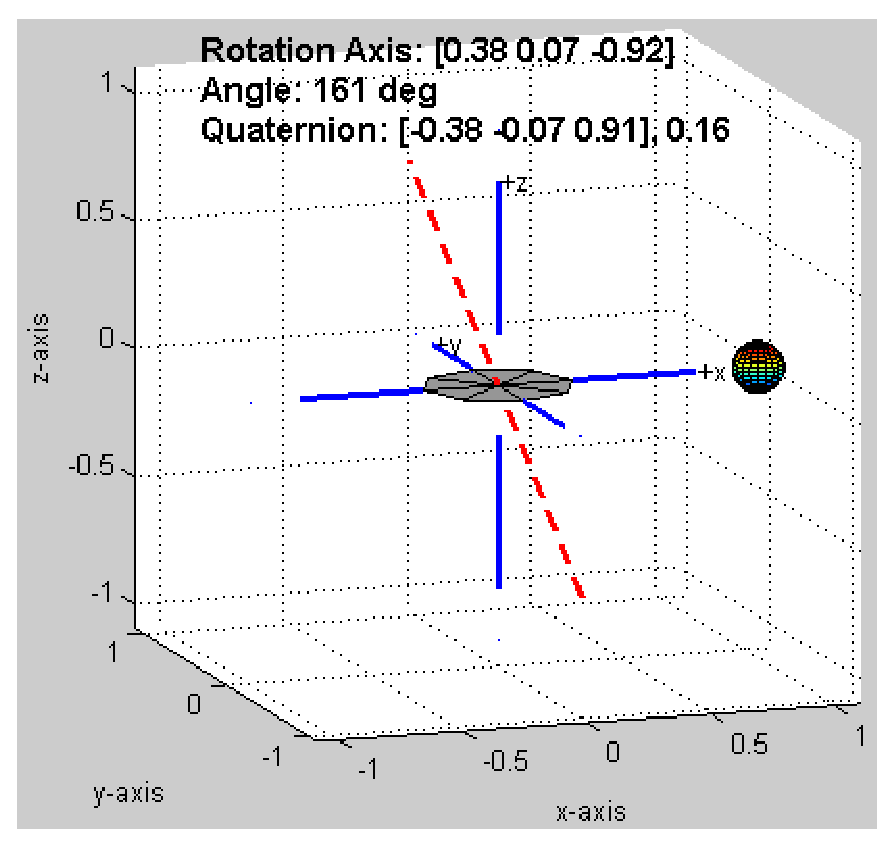
\psfig{file=figures/q_rotation_start.eps,height=3in}}
  \caption{TableSat Wireframe}
  \label{fig:TSatWireframe}
\end{figure}

The collection of the points in the TableSat wireframe can be rotated as the single point was from above.  Once new locations are determined, the TableSat wireframe can be redrawn visualizing the estimated current orientation of the TableSat (Figure \ref{fig:TSatWireframeEstimatedAttitude}).  Chapter \ref{chap:SoftwareDevelopmentforExperimentalIntegration} will cover the ``run-time'' visualizations in greater detail to show how as the estimator is running, updates to the estimated state, $\bs{\hat{x}}$, can be used to update the wireframe's orientation.

\begin{figure}[H]
  \centerline{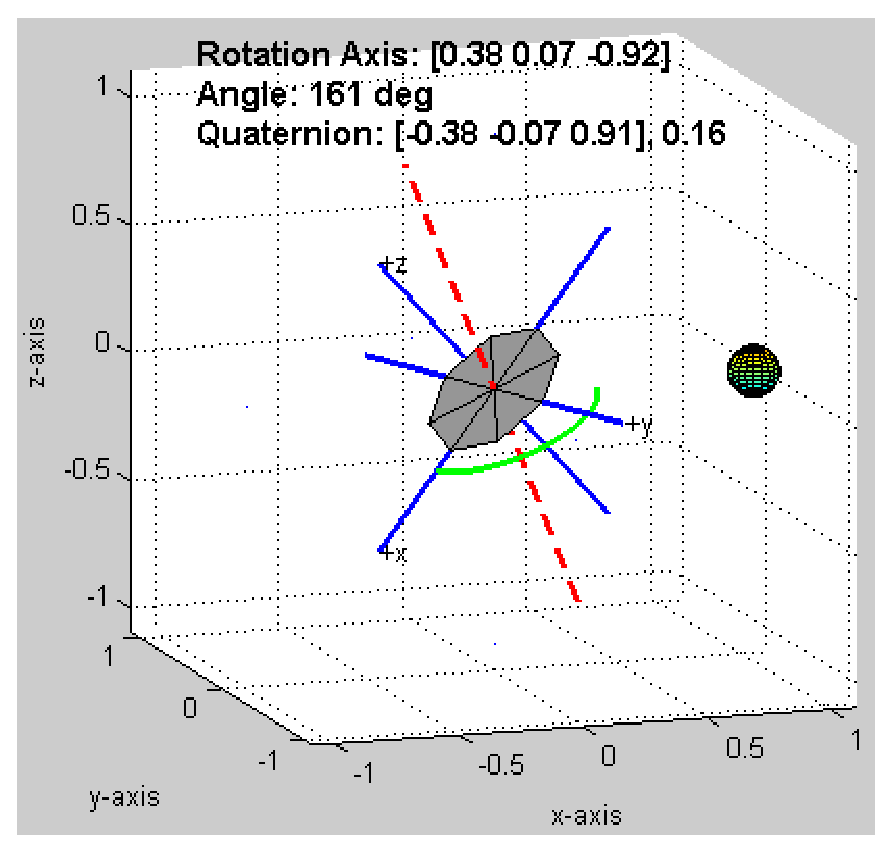
\psfig{file=figures/q_rotation_end.eps,height=3in}}
  \caption{TableSat Wireframe Estimated Attitude}
  \label{fig:TSatWireframeEstimatedAttitude}
\end{figure}


\subsubsection{Incremental Quaternion Rotations}
\label{subsubsec:IncrementalQuaternionRotations}

The quaternion's definition based on Euler's theorem of a rotation about a single axis makes tracking the orientation of a spin stabilized satellite an easier process.  NASA's MMS mission has a target spin rate of 3 rpm (~0.314 rad/sec).  A rotational quaternion representing the per second rotation about the z-axis is

\begin{equation}
  \begin{aligned}
    \bs{q}_{rps} = & ( 0\bs{i} + 0\bs{j} + 1\bs{k} ) \sin \left( \frac{-0.314}{2} \right) + \cos \left( \frac{-0.314}{2} \right) \\
    = & 0\bs{i} +0\bs{j} -0.156434\bs{k} + 0.987688
  \end{aligned}
\end{equation}

In an open loop system, the best estimate of the systems state would be to apply the quaternion rotation each second to the previous steps state starting with an initially known orientation.  For example if we have the TableSat at a $+1/4$ turn about the z-axis, each second we can calculate the best guess at the current attitude using just a quaternion multiplication.

\begin{equation}
  \begin{aligned}
    \bs{q}(t_{k+1}) = & \bs{q}_{rps} \otimes \bs{q}(t_{k}) \\
    \text{where } \bs{q}(t_0) = & 0 \bs{i} +0 \bs{j} -0.707107 \bs{k} +0.707107
  \end{aligned}
  \label{eqn:3rpmQuaternionEquation}
\end{equation}

\subsubsection{Quaternion Decomposition}
\label{subsubsec:QuaternionDecomposition}

The attitude of TSat is represented by a single quaternion.  The change in attitude between two states can be modeled by the a rotation about a single axis.  Figure \ref{fig:PreDecomposedQuaternion} show the attitude of a system described by the quaternion $\bs{q} = [\alpha, \beta, \phi], 0.16953$ which is a rotation of 2.8 radians about the axis $[\alpha, \beta, \phi]^T$.  For control purposes, decomposing the single quaternion into one representing a rotation about the z-axis and a second rotation about an axis in the x-y plane as shown in Figure \ref{fig:PostDecomposedQuaternion}.

\begin{figure}[H]
  \begin{subfigure}[h!]{0.5\textwidth}
    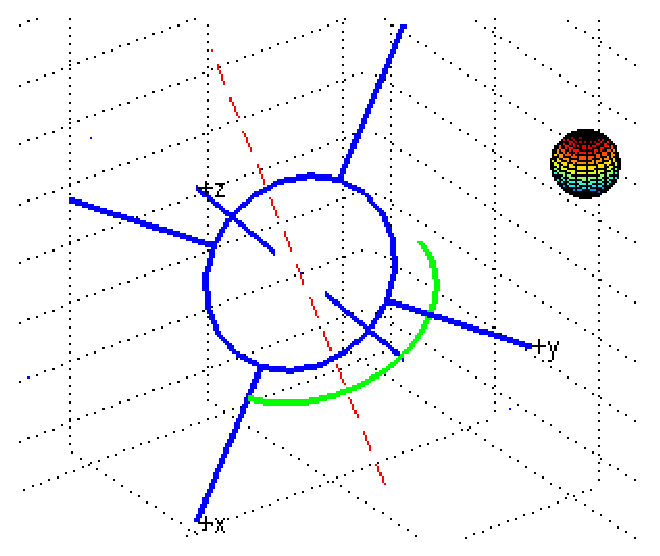
\includegraphics[width=\textwidth]{figures/quaternion_decompose_pre.eps}
    \caption{Quaternion State}
    \label{fig:PreDecomposedQuaternion}
  \end{subfigure}
  ~
  \begin{subfigure}[h!]{0.5\textwidth}
    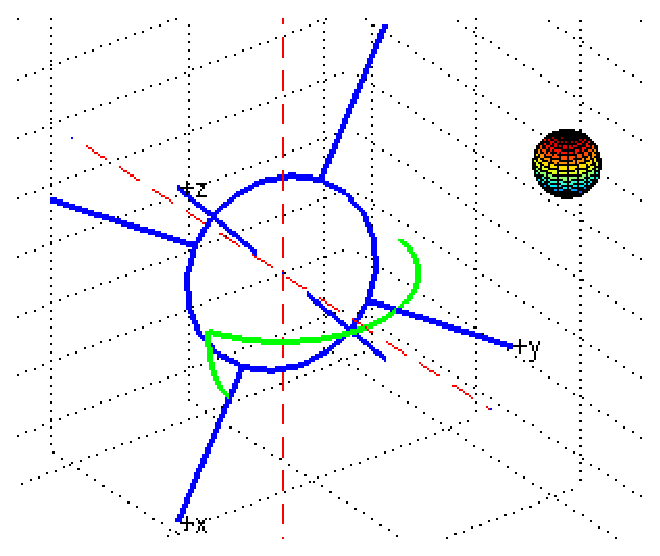
\includegraphics[width=\textwidth]{figures/quaternion_decompose_post.eps}
    \caption{Decomposed State}
    \label{fig:PostDecomposedQuaternion}
  \end{subfigure}
  \caption{Decomposing a Quaternion into Rotation and Nutation}
  \label{fig:QuaternionDecomposition}
\end{figure}

The quaternion that describes TSat's attitude $\bs{q}$ can be written as a sequence of two rotations.  A quaternion rotation about the z-axis $\bs{q_r}$ followed by the quaternion rotation about an axis in the x-y plane that creates a nutation $\bs{q_n}$.  Resultant rotations are performed through a left quaternion multiplication.
\begin{equation}
  \bs{q} = \bs{q_n} \otimes \bs{q_r} = \begin{bmatrix} \bs{v}_n \\ q_{0n} \end{bmatrix} \otimes \begin{bmatrix} \bs{v}_r \\ q_{0r} \end{bmatrix}
\end{equation}
\begin{equation}
  \begin{bmatrix}\bs{v} \\ q_{0} \end{bmatrix} =
  \begin{bmatrix} \bs{v}_n q_{0r} + \bs{v}_r q_{0n} + \bs{v}_n \times \bs{v}_r \\  q_{0n} q_{0r} - \bs{v}_n \cdot \bs{v}_r \end{bmatrix}
  \label{eqn:rot_nut_product}
\end{equation}
Expanding the vector components out creates the equation.
\begin{equation}
  \begin{bmatrix}
    q_{1} \\
    q_{2} \\
    q_{3} \\
    q_{0}
  \end{bmatrix}
  =
  \begin{bmatrix}
    \begin{bmatrix}
      q_{1n} \\
      q_{2n} \\
      q_{3n} \\
    \end{bmatrix} q_{0r} + \begin{bmatrix}
      q_{1r} \\
      q_{2r} \\
      q_{3r} \\
    \end{bmatrix} q_{0n} + \begin{bmatrix}
      q_{1n} \\
      q_{2n} \\
      q_{3n} \\
    \end{bmatrix} \times \begin{bmatrix}
      q_{1r} \\
      q_{2r} \\
      q_{3r} \\
    \end{bmatrix}
    \\
    q_{0n} q_{0r} - \begin{bmatrix}
      q_{1n} \\
      q_{2n} \\
      q_{3n} \\
    \end{bmatrix} \cdot \begin{bmatrix}
      q_{1r} \\
      q_{2r} \\
      q_{3r} \\
    \end{bmatrix} \\
  \end{bmatrix}
\end{equation}
and through simplification becomes
\begin{equation}
  \begin{bmatrix}
    q_{1} \\
    q_{2} \\
    q_{3} \\
    q_{0}
  \end{bmatrix}
  =
  \begin{bmatrix}
    q_{1n} q_{0r} + q_{1r} q_{0n} + q_{2n} q_{3r} - q_{3n} q_{2r} \\
    q_{2n} q_{0r} + q_{2r} q_{0n} + q_{3n} q_{1r} - q_{1n} q_{3r} \\
    q_{3n} q_{0r} + q_{3r} q_{0n} + q_{1n} q_{2r} - q_{2n} q_{1r} \\
  q_{0n} q_{0r} - (q_{1n} q_{1r} + q_{2n} q_{2r} + q_{3n} q_{3r} ) \\
  \end{bmatrix}
  \label{eqn:rot_nut_product_simplified}
\end{equation}
Now that we have an expanded representation of the resultant quaternion, we can use the restriction from the desired spin stabilized state for TableSat/MMS.  The rotational quaternion is allowed to move freely about the $z$-axis but should not have any displacement about the $x$ and $y$ axes.  From Equation \ref{eqn:RotationalQuaternionDefinition}, $q_{1r} = q_{2r} = 0$.
\begin{equation}
  \bs{q_{r}}
  = q_{1r} \bs{i} + q_{2r} \bs{j} + q_{3r} \bs{k} + q_{0r}
  = 0 \bs{i} + 0 \bs{j} + q_{3r} \bs{k} + q_{0r}
  \label{eqn:rotation_quaternion_defined}
\end{equation}
The nutation quaternion has the opposite restrictions where rotation is allowed about the $x$ and $y$ axes but not about the $z$ axis.  From Equation \ref{eqn:RotationalQuaternionDefinition}, $q_{3n} = 0$.
\begin{equation}
  \bs{q_{n}}
  = q_{1n} \bs{i} + q_{2n} \bs{j} + q_{3n} \bs{k} + q_{0n}
  = q_{1n} \bs{i} + q_{2n} \bs{j} + 0 \bs{k} + q_{0n}
  \label{eqn:nutation_quaternion_defined}
\end{equation}
Substituting equations \eqref{eqn:rotation_quaternion_defined} and \eqref{eqn:nutation_quaternion_defined} into \eqref{eqn:rot_nut_product_simplified} yields.
\begin{equation}
  \begin{bmatrix}
    q_{1} \\
    q_{2} \\
    q_{3} \\
    q_{0}
  \end{bmatrix}
  =
  \begin{bmatrix}
    q_{1n} q_{0r} + 0             + q_{2n} q_{3r} - 0 \\
    q_{2n} q_{0r} + 0             + 0             - q_{1n} q_{3r} \\
    0             + q_{3r} q_{0n} + 0             - 0 \\
  q_{0n} q_{0r} - (q_{1n} 0 + q_{2n} 0 + 0 q_{3r} ) \\
  \end{bmatrix}
\end{equation}
\begin{subequations}
  \begin{align}
    q_{1} &= q_{1n} q_{0r} + q_{2n} q_{3r} \label{eqn:rot_nut_1_1} \\
    q_{2} &= q_{2n} q_{0r} - q_{1n} q_{3r} \label{eqn:rot_nut_1_2} \\
    q_{3} &= q_{3r} q_{0n} \label{eqn:rot_nut_1_3} \\
    q_{0} &= q_{0n} q_{0r} \label{eqn:rot_nut_1_0}
  \end{align}
\end{subequations}
Solving \ref{eqn:rot_nut_1_3} and \ref{eqn:rot_nut_1_0} for $q_{3r}$ and $q_{0r}$ and substituting into \ref{eqn:rot_nut_1_1} and \ref{eqn:rot_nut_1_2}
\begin{subequations}
  \begin{align}
    q_{0n} q_{1} &= q_{1n} q_{0} + q_{2n} q_{3} \label{eqn:rot_nut_2_1} \\
    q_{0n} q_{2} &= q_{2n} q_{0} - q_{1n} q_{3} \label{eqn:rot_nut_2_2}
  \end{align}
\end{subequations}
combining \ref{eqn:rot_nut_2_1} and \ref{eqn:rot_nut_2_2}
\begin{equation}
  0 = (q_{0}q_{2} + q_{1}q_{3}) q_{1n} + (q_{2}q_{3} - q_{0}q_{1}) q_{2n}
\end{equation}
\begin{subequations}
  \begin{align}
    q_{1n} &= Q \cdot q_{2n} \\
    \text{where } Q &= \frac{q_{0}q_{1} - q_{2}q_{3}}{q_{0}q_{2} + q_{1}q_{3}}
  \end{align}
  \label{eqn:nutation_parameter_ratio}
\end{subequations}
The additional restriction than rotational quaternions have a unit norm can be leveraged in finding solutions
\begin{equation}
  \left\| \bs{q} \right\| = \sqrt{\bs{v} \cdot \bs{v} + q_0^2} = \sqrt{q_1^2+q_2^2+q_3^2+q_0^2}
  \label{eqn:quaternion_norm}
\end{equation}
Taking the norm of the rotational quaternion in Equation \ref{eqn:rotation_quaternion_defined} and substituting $q_{3r}$ and $q_{0r}$ from Equations \ref{eqn:rot_nut_1_3} and \ref{eqn:rot_nut_1_0} becomes
\begin{equation}
  (0)^2 + (0)^2 + \left( \frac{q_3}{q_{0n}} \right)^2 + \left( \frac{q_0}{q_{0n}} \right)^2 = 1
\end{equation}
solving for $q_{n0}$
\begin{equation}
  q_{n0} = \pm \sqrt{q_3^2 + q_0^2}
  \label{eqn:nutation_scalar}
\end{equation}
substituting \ref{eqn:nutation_parameter_ratio} and \ref{eqn:nutation_scalar} into \ref{eqn:nutation_quaternion_defined}
\begin{equation}
  \bs{q_{n}}
  = Q \cdot q_{2n} \bs{i} + q_{2n} \bs{j} + 0 \bs{k} \pm \sqrt{q_3^2 + q_0^2}
\end{equation}
and as this is a rotational quaternion, its norm should always equal one
\begin{equation}
  (Q \cdot q_{2n})^2 + (q_{2n})^2 + (q_3^2 + q_0^2) = 1
\end{equation}
which can be solved for the nutation quaternion's $q_{2n}$ term
\begin{equation}
  q_{2n} = \pm \sqrt{ \frac{1  - q_3^2 - q_0^2}{Q^2 + 1} }
  \label{eqn:qn2_solution}
\end{equation}

We now have a mapping of the original state quaternion $\bs{q}$ to its decomposed rotation $\bs{q}_r$ and nutation $\bs{q}_n$ quaternions.  The ability to break the attitude parameters into these two quantities is particularly useful for spin-stabilized satellites as it decouples the rate and attitude controllers.  Normally the attitude controller would need to propagate the desired quaternion attitude with input from the body rates. In this approach, the controller can ignore continuously changing rotational component $\bs{q}_r$, and limit its focus on driving the nutation error $\bs{q}_n$ to zero (Figure \ref{fig:PostDecomposedQuaternion}).
\begin{subequations}
  \begin{align}
    q_{1n} &= Q \cdot q_{2n} \\
    q_{2n} &= \sqrt{ \frac{1  - q_3^2 - q_0^2}{Q^2 + 1} }\\
    q_{n0} &= \sqrt{q_3^2 + q_0^2} \\
    q_{3r} &= \frac{q_3}{q_{0n}} \\
    q_{0r} &= \frac{q_0}{q_{0n}} \\
    \text{where } Q &= \frac{q_{0}q_{1} - q_{2}q_{3}}{q_{0}q_{2} + q_{1}q_{3}}
  \end{align}
\end{subequations}


\section{Satellite Dynamics}
\label{sec:SatelliteDynamics}

The goal in creating an accurate satellite dynamics model is it's ability to predict the state of the system given the last know state, the elapsed time since the last known state, and any inputs or disturbances to the system.  The initial scope of predicting the satellite's state is restricting it to a state propagation problem where only last state and elapsed time are considered.  Estimation techniques in Section \ref{chap:Estimators} will cover how a propagated state can be adjusted using the measured state.

\subsection{System Clock}
\label{subsec:SystemClock}

As was mentioned at the end of section \ref{subsubsec:IncrementalQuaternionRotations}, perfectly timed updates are highly unlikely.  Small variations in the timestep size will cause predicted state errors.  A state update running every 1.0001 seconds instead of every second would accumulate over a six degree error after tracking TableSat's state for an hour.  Linearized model would also be affected because the expected timestep size is incorporated as part of the discretization processes.

The preset fixed timestep is also not very fault tolerant.  When controlling the state of a stable, slow moving system the state tracking rate could be slowed down to conserve system resources.  In this circumstance a missed or series of missed updates due to faults can cause the predicted state to be several $\Delta t$ behind where it should be.  A solution built for variable steps can improve the robustness against these errors.

The ability to slow down a simulation to closely watch the initial transient behavior followed speeding up the simulation to inspect long term stability hold benefits for both outreach and research purposes.  The TSatPy system was built with this idea in mind which addresses the previous two issues as the system by design needs to be able to smoothly transition between variations in step sizes in a single run.

\begin{equation}
  \begin{aligned}
    t_k =& \sum\limits_{i=0}^{k-1} r_i (\tau_{i+1} - \tau_i)\\
    \text{where } \tau =& \text{ real time} \\
    t_k =& \text{ simulation time at step }k
  \end{aligned}
  \label{eqn:SystemTime}
\end{equation}

The system clock defined in Equation \ref{eqn:SystemTime} starts at zero and accumulates time depending on the set rate.

\subsection{Body Rate and Quaternion Propagation}
\label{subsec:BodyRateQuaternionPropagation}

Predicting the body rates, $\omega_x, \omega_y, \omega_z$, for TableSat requires knowledge about the body dynamics, the last calculated body rate, time elapsed since last update, and any applied moments.  Equation \ref{eqn:DiscreteEulerMomentEquations} is used to propagate the body rate in a variable step.

In Chapter \ref{chap:ObserverBasedControls} these quaternion and body rate propagation techniques will be incorporated into the observer based control system.


\chapter{TableSat 1A}
\label{chap:TableSat1A}


\chapter{TSatPy - TableSat Python Base Station}
\label{chap:TSatPy}



\chapter{STATE ERROR}
\label{chap:StateError}

A process for quantifying the error between two states is fundamental in any estimation or control techniques.  For the estimation case, it's the error $\bs{\hat{x}}_e$ between the measured state $\bs{x}$ and the estimated state $\bs{\hat{x}}$.  For the controllers, it's the error $\bs{x}_e$ representing the offset between the estimated state $\bs{\hat{x}}$ and the desired system state $\bs{x}_d$.

\begin{subequations}
  \begin{align}
    \bs{\hat{x}}_e &= \bs{\hat{x}} - \bs{x} \\
    \bs{x}_e &= \bs{\hat{x}} - \bs{x}_d
  \end{align}
  \label{eqn:StateError}
\end{subequations}

Sections \ref{sec:StateDifference} through \ref{subsec:ThetaMultiplierWithQuaternionVectorBalancing} outline the series of improvement made to the accuracy of the state error representation.  For comparison and to demonstrate their use with TSatPy, these sections will base their comparison on a single update to a proportional estimator.

\begin{equation}
  \bs{\hat{x}(t_{k+1})} = \bs{\hat{x}}(t_{k}) + \bs{K_p} ( \bs{\hat{x}}(t_{k}) - \bs{x}(t_{k}) )
  \label{eqn:PEstimatorStateDiff}
\end{equation}

This simple estimation technique has some notable deficiencies when applied to the attitude parameters of a spin stabilized satellite.  These parameters are expected to change as the satellite rotates, but this model has no method for predicting the change in parameters so will rely solely on the state error to correct $\bs{\hat{x}(t_{k+1})}$.  After an adequate method is established for calculating the state error, later sections will address improving upon the proportional estimator.

The sample error calculation in this section will be based off a last estimated state, $\bs{\hat{x}}(t_{k})$, of a $190^o$ rotation about $+z$-axis and a body rate of $\omega_z = 3$ rad/sec.  The associated the measured state, $\bs{x}(t_{k})$, is a $44^o$ rotation about the axis $0 \bs{i} + 0.1 \bs{j} + 1\bs{k}$ and a body rate of $\omega_z = 3.1$ rad/sec.


\begin{subequations}
  \begin{align}
    \bs{\hat{x}}(t_{k})
    = \begin{bmatrix}  \bs{\hat{q}}(t_{k}) \\ \bs{\hat{\omega}}(t_{k}) \end{bmatrix}
    &= \begin{bmatrix} 0 \bs{i} +0 \bs{j} -0.996195 \bs{k} -0.0871557 \\ 0 \bs{i} +0 \bs{j} +3 \bs{k} \end{bmatrix}\\
    \bs{x}(t_{k})
    = \begin{bmatrix}  \bs{q}(t_{k}) \\ \bs{\omega}(t_{k}) \end{bmatrix}
    &= \begin{bmatrix} 0 \bs{i} -0.0372747 \bs{j} -0.372747 \bs{k} +0.927184 \\ 0 \bs{i} +0 \bs{j} +3.1 \bs{k} \end{bmatrix}
  \end{align}
  \label{eqn:StateDifferenceQuaternionSamples}
\end{subequations}

\begin{singlespace}
  \begin{minted}[mathescape,linenos,numbersep=10pt,frame=lines,framesep=2mm]{python}
from TSatPy.State import Quaternion, QuaternionError, State, BodyRate
import numpy as np

x_hat = State(
    Quaternion([0,0,1],radians=190/180.0*np.pi),
    BodyRate([0,0,3]))
x_m = State(
    Quaternion([0,0.1,1],radians=44/180.0*np.pi),
    BodyRate([0,0,3.1]))
print("x_hat:  %s" % (x_hat))
print("x_m:    %s" % (x_m))

# Prints Out
# x_hat:  <Quaternion [-0 -0 -0.996195], -0.0871557>,
#         <BodyRate [0 0 3]>
# x_m:    <Quaternion [-0 -0.0372747 -0.372747], 0.927184>,
#         <BodyRate [0 0 3.1]>
  \end{minted}
\nocite{minted}
\end{singlespace}

Section \ref{sec:StateDifference} will start out with the standard element wise matrix difference to represent the state error.

\section{State Difference}
\label{sec:StateDifference}

The standard method for calculating the state error in either an estimation or control method is to calculate an element-wise difference.  TableSat has a seven element state in matrix form and expanding Equation \ref{eqn:StateError} becomes

\begin{equation}
  \begin{aligned}
    \bs{\hat{x}}_e(t_{k}) &= \begin{bmatrix}  \bs{\hat{q}}_e(t_{k}) \\ \bs{\hat{\omega}}_e(t_{k}) \\ \end{bmatrix} \\
    &= \begin{bmatrix} (\hat{q}_1 - q_{1}) \bs{i} + (\hat{q}_2 - q_{2}) \bs{j} + (\hat{q}_3 - q_{3}) \bs{k} + \hat{q}_0 - q_{0} \\ (\hat{\omega}_x - \omega_{x}) \bs{i} + (\hat{\omega}_y - \omega_{y}) \bs{j} + (\hat{\omega}_z - \omega_{z}) \bs{k} \end{bmatrix}
  \end{aligned}
  \label{eqn:StateDifference}
\end{equation}


Calculating the difference between the example estimated and measured states in Equation \ref{eqn:StateDifferenceQuaternionSamples} yields a state difference of

\begin{equation}
  \begin{aligned}
    \bs{\hat{x}}_e(t_{k})
    = \begin{bmatrix}  \bs{\hat{q}}_e(t_{k}) \\ \bs{\hat{\omega}}_e(t_{k}) \end{bmatrix}
    &= \begin{bmatrix} 0 \bs{i} +0.0372747 \bs{j} -0.623447 \bs{k} -1.01434 \\ 0 \bs{i} +0 \bs{j} -0.1 \bs{k} \end{bmatrix}
  \end{aligned}
  \label{eqn:StateDifferenceSample}
\end{equation}


\begin{singlespace}
  \begin{minted}[mathescape,linenos,numbersep=10pt,frame=lines,framesep=2mm]{python}
x_e = State(
    Quaternion(x_hat.q.vector - x_m.q.vector,
        x_hat.q.scalar - x_m.q.scalar),
    x_hat.w - x_m.w)
print("x_e:  %s" % (x_e))

# Prints Out
# x_e:  <Quaternion [0 0.0372747 -0.623447], -1.01434>,
#       <BodyRate [0 0 -0.1]>
  \end{minted}
\nocite{minted}
\end{singlespace}


The body rate error calculations are well behaved and are able to be directly used with standard estimation based control techniques.  The difference in quaternion parameters however pose a number of problems even when used in a basic proportional estimator.  Using this method of error measurement will be difficult especially since after a cursory review the scalar quantity in the error quaternion that is outside the possible range for a rotational quaternion.  Section \ref{sec:QuaternionDifference} will attempt to use this state difference along with a standard proportional estimation technique.

\section{Quaternion Difference}
\label{sec:QuaternionDifference}

Taking the quaternion difference from Equation \ref{eqn:StateDifferenceSample}, and incorporating into the proportional estimation correction in Equation \ref{eqn:PEstimatorStateDiff} produces an state adjustment and estimated attitude of

\begin{equation}
  \begin{aligned}
    \bs{q}_{adj} = -0.8 \cdot \bs{q}_e =& -0.8 \cdot (0 \bs{i} + 0.0372747 \bs{j} -0.623447 \bs{k} -1.01434 ) \\
                       =& 0 \bs{i} -0.0298198 \bs{j} +0.498758 \bs{k} +0.811472 \\
    \bs{\hat{q}(t_{k+1})} =& \bs{\hat{q}(t_{k})} + \bs{q}_{adj} \\
                       =& 0 \bs{i} -0.0298198 \bs{j} -0.497437 \bs{k} + 0.724316 \\
  \end{aligned}
\end{equation}

\begin{singlespace}
  \begin{minted}[mathescape,linenos,numbersep=10pt,frame=lines,framesep=2mm]{python}
q_hat = x_hat.q
q_e = x_e.q
q_adj = Quaternion(-0.8 * q_e.vector, -0.8 * q_e.scalar)
q_hat_new = Quaternion(q_hat.vector + q_adj.vector,
        q_hat.scalar + q_adj.scalar)

print("q_e:         %s" % (q_e))
print("q_adj:       %s" % (q_adj))
print("q_hat_new:   %s" % (q_hat_new))
print("|q_hat_new|: %g" % (q_hat_new.mag))

# Prints Out
# q_e:         <Quaternion [0 0.0372747 -0.623447], -1.01434>
# q_adj:       <Quaternion [-0 -0.0298198 0.498758], 0.811472>
# q_hat_new:   <Quaternion [-0 -0.0298198 -0.497437], 0.724316>
# |q_hat_new|: 0.879185
  \end{minted}
\nocite{minted}
\end{singlespace}

The new estimate for the quaternion attitude has been adjusted closer to the measured state although the newly estimated state has a norm of $ \| \bs{\hat{q}(t_{k+1})} \| = 0.879185$.  Since failing to conform to the unit magnitude for rotational quaternions, this newly estimated attitude quaternion corrupts the systems state especially over multiple steps and long simulations.  For rotational quaternions with norms less that the unit quaternion the rotated points end up converging into the origin.  If the adjustment ends up with a rotational quaternion larger than a unit magnitude, rotated points dilate away from the origin.

\begin{singlespace}
  \begin{minted}[mathescape,linenos,numbersep=10pt,frame=lines,framesep=2mm]{python}
pt = np.mat([[1,0,0]])
pt = q_hat_new.rotate_points(pt)
print("pt * pt.T:   %s" % (pt * pt.T))

# Prints Out
# pt * pt.T:   [[ 0.5974769]]
  \end{minted}
\nocite{minted}
\end{singlespace}


\section{Scaled Quaternion Difference}
\label{sec:ScaledQuaternionDifference}

The next step to correct for the dilation or compression of points is to scale the adjusted quaternion to a unit quaternion before using it to represent the system's state.  The quaternion can be scaled through a standard vector normalization.

\begin{equation}
  \bs{\hat{q}}_n = \frac{\bs{q}_v + q_0}{\sqrt{\bs{q}_v \bullet \bs{q}_v + q_0^2}}
  \label{eqn:NormalizeQuaternion}
\end{equation}

\begin{singlespace}
  \begin{minted}[mathescape,linenos,numbersep=10pt,frame=lines,framesep=2mm]{python}
print("q_hat_new:   %s" % (q_hat_new))
q_hat_new.normalize()
print("q_hat_new:   %s" % (q_hat_new))
print("|q_hat_new|: %g" % (q_hat_new.mag))

# Prints Out
# q_hat_new:   <Quaternion [-0 -0.0298198 -0.497437], 0.724316>
# q_hat_new:   <Quaternion [-0 -0.0339175 -0.565793], 0.823849>
# |q_hat_new|: 1
  \end{minted}
\nocite{minted}
\end{singlespace}

The newly estimated state is equivalent to a $69$ degree rotation about
\begin{equation}\hat{\bs{e}} = \begin{bmatrix} 0 & -0.0598395 & -0.998208 \end{bmatrix}\end{equation}.  While this state estimate conforms to the unit quaternion requirement and will no longer corrupt rotations, it has little in common with the desired $0.8$ proportional gain used the estimator's design.

\begin{singlespace}
  \begin{minted}[mathescape,linenos,numbersep=10pt,frame=lines,framesep=2mm]{python}
e, r = q_hat_new.to_rotation()
print("e: <%g, %g, %g>\ndegree: %g" % (
    e[0,0],e[1,0],e[2,0], r * 180.0 / np.pi))

# Prints Out
# e: <-0, -0.0598395, -0.998208>
# degree: 69.056
  \end{minted}
\nocite{minted}
\end{singlespace}


\section{Quaternion Multiplicative Error}
\label{sec:QuaternionMultiplicativeError}

The previous sections have established that the state difference approach for adjusting for errors in attitude measurements has significant issues especially for low frequency updates with high error values.  The quaternion multiplication defined in Equation \ref{eqn:QuaternionMultiplication} can be used to modify the attitude while not introducing corruption into the model if used with rotational unit quaternions.

If the estimated and measured states converge with the multiplicative correction, the error quaternion should converge to the identity quaternion.  The identity quaternion as with the identity matrix is the quantity that when multiplied by another quaternion, does not modify its value.  This identity holds true for general as well as rotational quaternions.

\begin{equation}
  \bs{q}_I = 0 \bs{i} + 0 \bs{j} + 0 \bs{k} + 1
\end{equation}

An Identity function was created it the TSatPy.State module to construct an identity quaternion.

\begin{singlespace}
  \begin{minted}[mathescape,linenos,numbersep=10pt,frame=lines,framesep=2mm]{python}
from TSatPy import State

q = State.Quaternion([1,2,3], 4)
print("q       = %s" % q)
q_I = State.Identity()
print("q_I     = %s" % q_I)
print("q_I * q = %s" % (q_I * q))

# Prints Out
# q       = <Quaternion [1 2 3], 4>
# q_I     = <Quaternion [0 0 0], 1>
# q_I * q = <Quaternion [1 2 3], 4>
  \end{minted}
  \nocite{minted}
\end{singlespace}

Rotational quaternions are considered equal if they represent the same attitude.  The same attitude can be represented by more than one distinct quaternions, so a strict equality is not adequate.  The test for equality can be done by using the quaternion conjugate $\bs{q}^*$.

\begin{subequations}
  \begin{align}
    \bs{\hat{q}} = \bs{q} & \iff \bs{\hat{q}}^* \otimes \bs{q} = \bs{q}^* \otimes \bs{\hat{q}} = \bs{q}_I \text{ or } -\bs{q}_I \\
    \text{where } \bs{q}^* &= \begin{bmatrix} -\bs{v} \\ q_0 \end{bmatrix}
  \end{align}
  \label{eqn:QuaternionEquality}
\end{subequations}

The sample below shows how two distinct quaternions can represent the same attitude and that Equation \ref{eqn:QuaternionEquality} holds true.

\begin{singlespace}
  \begin{minted}[mathescape,linenos,numbersep=10pt,frame=lines,framesep=2mm]{python}
a = Quaternion([0,0,1],radians=190/180.0*np.pi)
b = Quaternion([0,0,1],radians=(190 + 360)/180.0*np.pi)

print("a:          %s" % (a))
print("b:          %s" % (b))
print("a.conj * b: %s" % (a.conj * b))

# Prints Out
# a:          <Quaternion [-0 -0 -0.996195], -0.0871557>
# b:          <Quaternion [0 0 0.996195], 0.0871557>
# a.conj * b: <Quaternion [0 0 -3.46945e-16], -1>
  \end{minted}
\nocite{minted}
\end{singlespace}

Equation \ref{eqn:QuaternionEquality} provides a method for determining whether two quaternions represent the same attitude, it can also be used to quantify the difference between two rotational quaternions using the multiplicative comparison.

\begin{equation}
  \bs{q}_e = \bs{q}^* \otimes \bs{\hat{q}}
  \label{eqn:QuaternionError}
\end{equation}

Continuing with the example measured and estimated states from Equation \ref{eqn:StateDifferenceQuaternionSamples}, the multiplicative quaternion error between these states evaluates to

\begin{equation}
  \begin{aligned}
    \bs{q}_e = & \bs{q}^* \otimes \bs{\hat{q}} \\
    = & \big( 0 \bs{i} -0.0372747 \bs{j} -0.372747 \bs{k} +0.927184 \big)^* \\
    & \otimes \big( 0 \bs{i} +0 \bs{j} -0.996195 \bs{k} -0.0871557 \big)\\
    = & -0.0371329 \bs{i} -0.00324871 \bs{j} -0.956143 \bs{k} +0.29052
  \end{aligned}
  \label{eqn:QuaternionErrorSample}
\end{equation}

The sample error measurement in Equation \ref{eqn:QuaternionErrorSample} relates well to the deviations in the estimated and measured attitudes as it represents a 146 degree rotation about the Euler axis $<-0.0388067, -0.00339514, -0.999241>$ which would rotate the estimated quaternion back to match up perfectly with the measured state.  The multiplicative error correction quaternion also solves the issue encountered in Section \ref{sec:QuaternionDifference} where the magnitude of the error quaternion did not remain fixed at the unit quaternion.

\begin{singlespace}
  \begin{minted}[mathescape,linenos,numbersep=10pt,frame=lines,framesep=2mm]{python}
from TSatPy.State import QuaternionError
q_e = QuaternionError(x_hat.q, x_m.q)

print("q_e:   %s" % (q_e))
print("|q_e|: %s" % (q_e.mag))
e, r = q_e.to_rotation()
print("e:     <%g, %g, %g>\ndegree: %g" % (
    e[0,0],e[1,0],e[2,0], r * 180.0 / np.pi))

# Prints Out
# q_e:   <Quaternion [-0.0371329 -0.00324871 -0.956143], 0.29052>
# |q_e|: 1.0
# e:     <-0.0388067, -0.00339514, -0.999241>
# degree: 146.222
  \end{minted}
\nocite{minted}
\end{singlespace}

\section{Quaternion Multiplicative Correction}
\label{sec:QuaternionMultiplicativeCorrection}

Section \ref{sec:QuaternionMultiplicativeError} was able to establish a method for quantifying differences in attitudes in a method that preserves the integrity of the rotational quaternion while creating a representative measure of the state error.  For the next step, a series of options were investigated to determine how the error measurement can be used in estimation and control techniques.

\subsection{Parameter Multiplier}
\label{subsec:ParameterMultiplier}

With a parameter multiplier method, the four parameters of the error quaternion get scaled by a $\bs{K_p}$ term similar to the standard proportional adjustment.

\begin{equation}
  \bs{q}_{adj} = \bs{K_p} \bs{q}_e
    = \bs{K_p} \begin{bmatrix} \bs{v}_e \\ q_{e0} \end{bmatrix}
    = \begin{bmatrix} \bs{K_{vp}}\bs{v}_e \\ K_{0p} \cdot q_{e0} \end{bmatrix}
  \label{eqn:ParameterMultiplier}
\end{equation}

The $\bs{K_{vp}}$ term is a 3x3 matrix.  Since $\bs{v}_e$ defines the path between the estimated and measured quaternions the only form of $\bs{K_{vp}}$ that would not corrupt the direction mapped between the two states is

\begin{equation}
  \bs{K_{vp}} \bs{v}_e = \lambda \bs{v}_e
  \label{eqn:QuaternionVectorCorrection}
\end{equation}

The effect of the $\lambda$ parameter is to modify the magnitude of the quaternion's Euler axis but not modify it's direction.  Combining \ref{eqn:QuaternionVectorCorrection} with \ref{eqn:ParameterMultiplier} yields

\begin{equation}
  \bs{q}_{adj} = \begin{bmatrix} \lambda \bs{v}_e \\ K_{0p} \cdot q_{e0} \end{bmatrix}
  \label{eqn:QuaternionScalarMultiplier}
\end{equation}

Reducing the tunable parameters for the proportional quaternion estimator to $\lambda$ and $K_{0p}$.  This configuration, shares the same flaws as the state difference approach in Section \ref{sec:QuaternionDifference} where the magnitude of the adjusted quaternion can vary from the unit quaternion causing dilation or compression of rotated points.

\begin{singlespace}
  \begin{minted}[mathescape,linenos,numbersep=10pt,frame=lines,framesep=2mm]{python}
q_adj = Quaternion(
    q_e.vector * 0.7,  # lambda chosen as 0.7
    q_e.scalar * 0.4)  # K_p0 chosen as 0.4

print("q_adj:   %s" % (q_adj))
print("|q_adj|: %s" % (q_adj.mag))

# Prints Out
# q_adj:   <Quaternion [-0.025993 -0.0022741 -0.6693], 0.116208>
# |q_adj|: 0.679814272084
  \end{minted}
\nocite{minted}
\end{singlespace}


\subsection{Parameter Multiplier with Normalization}
\label{subsec:ParameterMultiplierwithNormalization}

Normalizing the paramater multiplier's adjustment quaternion resolves the issues with dilating and contracting points as it did in Section \ref{sec:ScaledQuaternionDifference}.  A normalized parameter multiplier quaternion does not suffer from an invalid Euler axis of rotation as in Section \ref{sec:ScaledQuaternionDifference} as only the magnitude of the quaternion's vector is modified.  The scalar quantity however still ends up being muddied due to the coupling between  and $K_{0p}$ that occurs via normalization.  A constant angular error and $K_{0p}$ can create varied adjustment values based on the selection of the $\lambda$ gain.

\subsection{$q_0$ Multiplier with Normalization}
\label{subsec:q0MultiplierWithNormalization}

Since the $\lambda$ gain used above provides no benefit and only ends up complicating the quaternion adjustment calculation, it can be dropped leaving a quaternion adjustment based solely on a modification of the scalar quantity.  After the scalar gain $k$, the quaternion can be normalized back to a unit quaternion.

\begin{equation}
  \begin{aligned}
  \bs{q}_{adj} = & \begin{bmatrix} \bs{v}_e / \alpha \\ ( k \cdot q_{e0} )  / \alpha \end{bmatrix} \\
  \text{where } \alpha & = \sqrt{\bs{v}_e^T \cdot \bs{v}_e + k^2 \cdot q_{e0}^2}
  \end{aligned}
  \label{eqn:ScalarMultiplierWithNormalization}
\end{equation}

Equation \ref{eqn:ScalarMultiplierWithNormalization} has a few strengths when used to apply adjustments to a quaternion attitude estimate.  It's based off the multiplicative correction quaternion that accurately quantifies the difference in estimated and measured states.  The normalization ensures that the rotational quaternion representation is not corrupted and when applied will not cause dilation or compression of the model.

The disadvantage to using this representation is that the quaternion scalar parameter is a nonlinear function of the rotation angle (Equation \ref{eqn:RotationalQuaternionDefinition}).  Applying a constant scalar multiplier to it will result in inconsistent adjustment amount depending on the position along the sinusoidal value.

\subsection{$\theta$ Multiplier with Quaternion Vector Balancing}
\label{subsec:ThetaMultiplierWithQuaternionVectorBalancing}

The section will cover the final version of the quaternion adjustment calculation that takes into consideration all the issues encountered in the above sections.  The function designated in this thesis for the scaling of a quaternion to for use with quaternion multiplicative corrections while maintaining it's connection to the physical system will be $\bs{\psi}(\bs{q}, k)$ where

\begin{equation}
  \begin{aligned}
    \bs{\psi}(\bs{q}, k) &= \begin{bmatrix} \bs{v} / \gamma \\ \cos ( k \cdot 2\cos^{-1} (q_0))  \end{bmatrix} \\
    \text{where } \gamma &= \sqrt{\frac{\bs{v}^T \cdot \bs{v}}{\sin^2 ( k \cdot 2\cos^{-1} (q_0))}} \\
    \bs{q} &= \begin{bmatrix} \bs{v} \\ q_0  \end{bmatrix}
  \end{aligned}
  \label{eqn:PSI}
\end{equation}

Using Equation \ref{eqn:PSI} to create a rotational quaternion adjustment for the proportional estimator would take the form.

\begin{equation}
  \bs{q}_{adj} = \bs{\psi}(\bs{q}_e, k)
  \label{eqn:PEstimatorAngleMultiplierwithVectorMagnitudeNormalization}
\end{equation}

The code snippet below demonstrates the usage of Equation \ref{eqn:PEstimatorAngleMultiplierwithVectorMagnitudeNormalization} with TSatPy.  The proposed error between the measured and estimated quaternions is constructed as a $45^o$ rotation about the body's $z$-axis.  With a chosen gain of 0.2, the expected quaternion adjustment is correct in evaluating to be a $9^o$ rotation about the $z$-axis that still conforms to the unit norm of a rotational quaternion.

\begin{singlespace}
  \begin{minted}[mathescape,linenos,numbersep=10pt,frame=lines,framesep=2mm]{python}
from TSatPy.State import Quaternion
import numpy as np

k = 0.2
degree = 45

q_e = Quaternion([0,0,1], radians=degree/180.0*np.pi)
print("q_e:     %s" % (q_e))

kpc = k * np.arccos(q_e.scalar)
gamma = np.sqrt((q_e.vector.T * q_e.vector)[0,0] / (np.sin(kpc))**2)

q_adj = Quaternion(
    q_e.vector / gamma,
    np.cos(kpc))
print("q_adj:   %s" % (q_adj))
print("|q_adj|: %s" % (q_adj.mag))

e, r = q_adj.to_rotation()
print("e:       <%g, %g, %g>\ndegree: %g" % (
    e[0,0],e[1,0],e[2,0], r * 180.0 / np.pi))

# Prints Out
# q_e:     <Quaternion [-0 -0 -0.382683], 0.92388>
# q_adj:   <Quaternion [-0 -0 -0.0784591], 0.996917>
# |q_adj|: 1.0
# e:       <-0, -0, -1>
# degree: 9
  \end{minted}
\nocite{minted}
\end{singlespace}

\section{High Integrity State Adjustments}
\label{sec:HighIntegrityStateAdjustments}

The work described in Sections \ref{sec:StateDifference} through \ref{subsec:ThetaMultiplierWithQuaternionVectorBalancing} have established a solid foundation to quantify the state error along with appropriate methods for scaling state errors.

Quaternion Error

\begin{equation}
  \bs{q}_e = \bs{q}^* \otimes \bs{\hat{q}}
\end{equation}

Adjustment Quaternions

\begin{equation}
  \begin{aligned}
    \bs{q}_{adj} &= \bs{\psi}(\bs{q}_e, K_{qp}) \\
    \text{where } \bs{\psi}(\bs{q}, k) &= \begin{bmatrix} \bs{v} / \gamma \\ \cos ( k \cdot 2\cos^{-1} (q_0))  \end{bmatrix} \\
    \gamma &= \sqrt{\frac{\bs{v}^T \cdot \bs{v}}{\sin^2 ( k \cdot 2\cos^{-1} (q_0))}} \\
    \bs{q} &= \begin{bmatrix} \bs{v} \\ q_0  \end{bmatrix}
  \end{aligned}
\end{equation}

Body Rate Error

\begin{equation}
  \bs{\omega}_e = \bs{\hat{\omega}} - \bs{\omega}
\end{equation}

Adjustment Body Rates

\begin{equation}
  \bs{\omega}_{adj} = \bs{K_{\omega p}} \bs{\omega}_e
\end{equation}

The following snippet will demonstrate the implementation of the chosen state parameterization and correction methods.  The state is created to represent a 44 degree rotation about the body's $z$-axis with body rates of $\omega_x, \omega_y, \omega_z = 0.02, -0.04, 0.3$ rad/sec.  The corrected state will take $1/4$ of the quaternion rotation and scale the body rates by 0.2, 0.3, and 0.8 respectively.

\begin{singlespace}
  \begin{minted}[mathescape,linenos,numbersep=10pt,frame=lines,framesep=2mm]{python}
from TSatPy.State import State, Quaternion, BodyRate
from TSatPy.StateOperator import QuaternionGain, BodyRateGain, StateGain
import numpy as np

k_q = 0.25
k_w = [[0.2,0,0],[0,0.3,0],[0,0,0.8]]

x = State(
    Quaternion([0,0,1],radians=44/180.0*np.pi),
    BodyRate([0.02,-0.04,0.3]))
print("x:      %s" % (x))

Kx = StateGain(
    QuaternionGain(k_q),
    BodyRateGain(k_w))
print("Kx:     %s" % (Kx))

x_adj = Kx * x
print("x_adj:  %s" % (x_adj))

e, r = x_adj.q.to_rotation()
print("e:      <%g, %g, %g>\ndegree: %g" % (
    e[0,0],e[1,0],e[2,0], r * 180.0 / np.pi))

# Prints Out
# x:      <Quaternion [-0 -0 -0.374607], 0.927184>,
#         <BodyRate [0.02 -0.04 0.3]>
# Kx:     <StateGain <Kq 0.25>,
#           <Kw = [[ 0.2 0. 0. ] [ 0. 0.3 0. ] [ 0. 0. 0.8]]>>
# x_adj:  <Quaternion [-0 -0 -0.0958458], 0.995396>,
#         <BodyRate [0.004 -0.012 0.24]>
# e:      <-0, -0, -1>
# degree: 11
  \end{minted}
\nocite{minted}
\end{singlespace}


\chapter{ESTIMATORS}
\label{chap:Estimators}

Section \ref{chap:StateError} explained the rationale for the state representations and how adjustments can be applied to them in a manner than preserves the integrity of it's connection to the TableSat's physical orientation.  Usage of the gains are also done to make the effects of gain tuning more intuitive.

\section{State Prediction}
\label{sec:StatePrediction}

Section \ref{sec:BodyRatePIDEstimation} shows that to keep accurate tracking of a spin-stabilized satellite like TableSat or MMS, the system's dynamic equations are required to couple the body rate and quaternion values.  This is especially important for the NASA MMS TableSat 1A implementation since only the magnetometer and coarse sun sensors provide feedback about the system's state, and they only have a partial measurement of the attitude quaternion and no direct measurement of the body rates.

The approach taken in the TSatPy code to create state predictions off previous state estimates is to start with a discretized Euler's Moment Equations \ref{eqn:DiscreteEulerMomentEquations} to predict $\bs{\dot{\omega}}(t_{k+1})$.  The the current estimated body rate is adjusted based on the variable time step size.

\begin{equation}
  \bs{\omega}(t_{k+1}) = \bs{\omega}(t_{k}) + \bs{\dot{\omega}}(t_{k+1})\cdot (t_{k+1} - t_k)
\end{equation}

The newly estimated body rates $\bs{\omega}(t_{k+1})$ are supplied to the discretized quaternion dynamics Equation \ref{eqn:DiscreteQuaternionPropagation} to calculate the newly estimated rotational quaternion.

\section{PID State Estimation}
\label{sec:BodyRatePIDEstimation}

This section covers the use of PID adjustments to track state estimation.  Section \ref{chap:StateError} covered how states and especially the quaternion portion can be scaled.  The same method can be applied to the proportional part of the PID estimator.

\subsection{Proportional State Estimation}
\label{subsec:ProportionalEstimator}

The proportional estimator defined in Equation \ref{eqn:PEstimator} was implemented in TSatPy.  Taking the estimated and measured states from Equation \ref{eqn:StateDifferenceQuaternionSamples}, an update of the TableSat state estimate is performed in the following manner.

\begin{subequations}
  \begin{align}
    \bs{\hat{x}}(t_{k+1}) &= \begin{bmatrix} \bs{\hat{q}}(t_{k+1}) \\ \bs{\hat{\omega}}(t_{k+1}) \end{bmatrix} = \begin{bmatrix} \bs{\psi}(\bs{q}_e(t_{k}), K_{qp}) \otimes \bs{\hat{q}}(t_{k}) \\  \bs{\hat{\omega}}(t_{k}) + \bs{K}_{\omega p} \cdot \bs{\omega}_e(t_{k}) \end{bmatrix}
  \end{align}
  \label{eqn:PEstimator}
\end{subequations}

\begin{singlespace}
  \begin{minted}[mathescape,linenos,numbersep=10pt,frame=lines,framesep=2mm]{python}
from TSatPy import StateOperator, Estimator, State
from TSatPy.Clock import Metronome
import numpy as np

x_ic = State.State(
    State.Quaternion([0,0,1],radians=190/180.0*np.pi),
    State.BodyRate([0,0,3]))
print("x_ic:    %s" % (x_ic))

k = 0.2
Kp = StateOperator.StateGain(
    StateOperator.QuaternionGain(k),
    StateOperator.BodyRateGain(np.eye(3) * k))
print("Kp:  %s" % (Kp))

c = Metronome()
pid = Estimator.PID(c, ic=x_ic)
pid.set_Kp(Kp)
print("pid: %s" % (pid))

x_m = State.State(
    State.Quaternion([0,0.1,1],radians=44/180.0*np.pi),
    State.BodyRate([0,0,3.1]))
pid.update(x_m)
print("pid.x_hat:   %s" % (pid.x_hat))

e, r = pid.x_hat.q.to_rotation()
print("e:      <%g, %g, %g>\ndegree: %g" % (
    e[0,0],e[1,0],e[2,0], r * 180.0 / np.pi))

# Prints Out
# x_ic:    <Quaternion [-0 -0 -0.996195], -0.0871557>,
#          <BodyRate [0 0 3]>
# Kp:  <StateGain <Kq 0.2>,
#      <Kw = [[ 0.2 0. 0. ] [ 0. 0.2 0. ] [ 0. 0. 0.2]]>>
# pid: PID
#  x_hat <Quaternion [-0 -0 -0.996195], -0.0871557>, <BodyRate [0 0 3]>
#  Ki None
#  Kp <StateGain <Kq 0.2>,
#     <Kw = [[ 0.2 0. 0. ] [ 0. 0.2 0. ] [ 0. 0. 0.2]]>>
#  Kd None
# pid.x_hat:   <Quaternion [-0.00170765 0.00968454 -0.985915], 0.16696>,
#              <BodyRate [0 0 3.02]>
# e:      <-0.00173196, 0.00982241, -0.99995>
# degree: 160.778
  \end{minted}
\nocite{minted}
\end{singlespace}

This demonstrates that a proportional estimator initialized to a state of a $190^o$ rotation about $+z$-axis and a body rate of $\omega_z = 3$ rad/sec.  The proportional gain applied to state errors is set to $0.2$ for the quaternion and all body rates.  After the measured state of a $44^o$ rotation about the axis $0 \bs{i} + 0.1 \bs{j} + 1\bs{k}$ and a body rate of $\omega_z = 3.1$ rad/sec is applied, the new estimated state is a $160.778^o$ degree rotation about $0.00173196 \bs{i} - 0.00982241 \bs{j} + 0.99995\bs{k}$ with a body rate of $3.02$ rad/sec.

\begin{figure}[H]
  \centerline{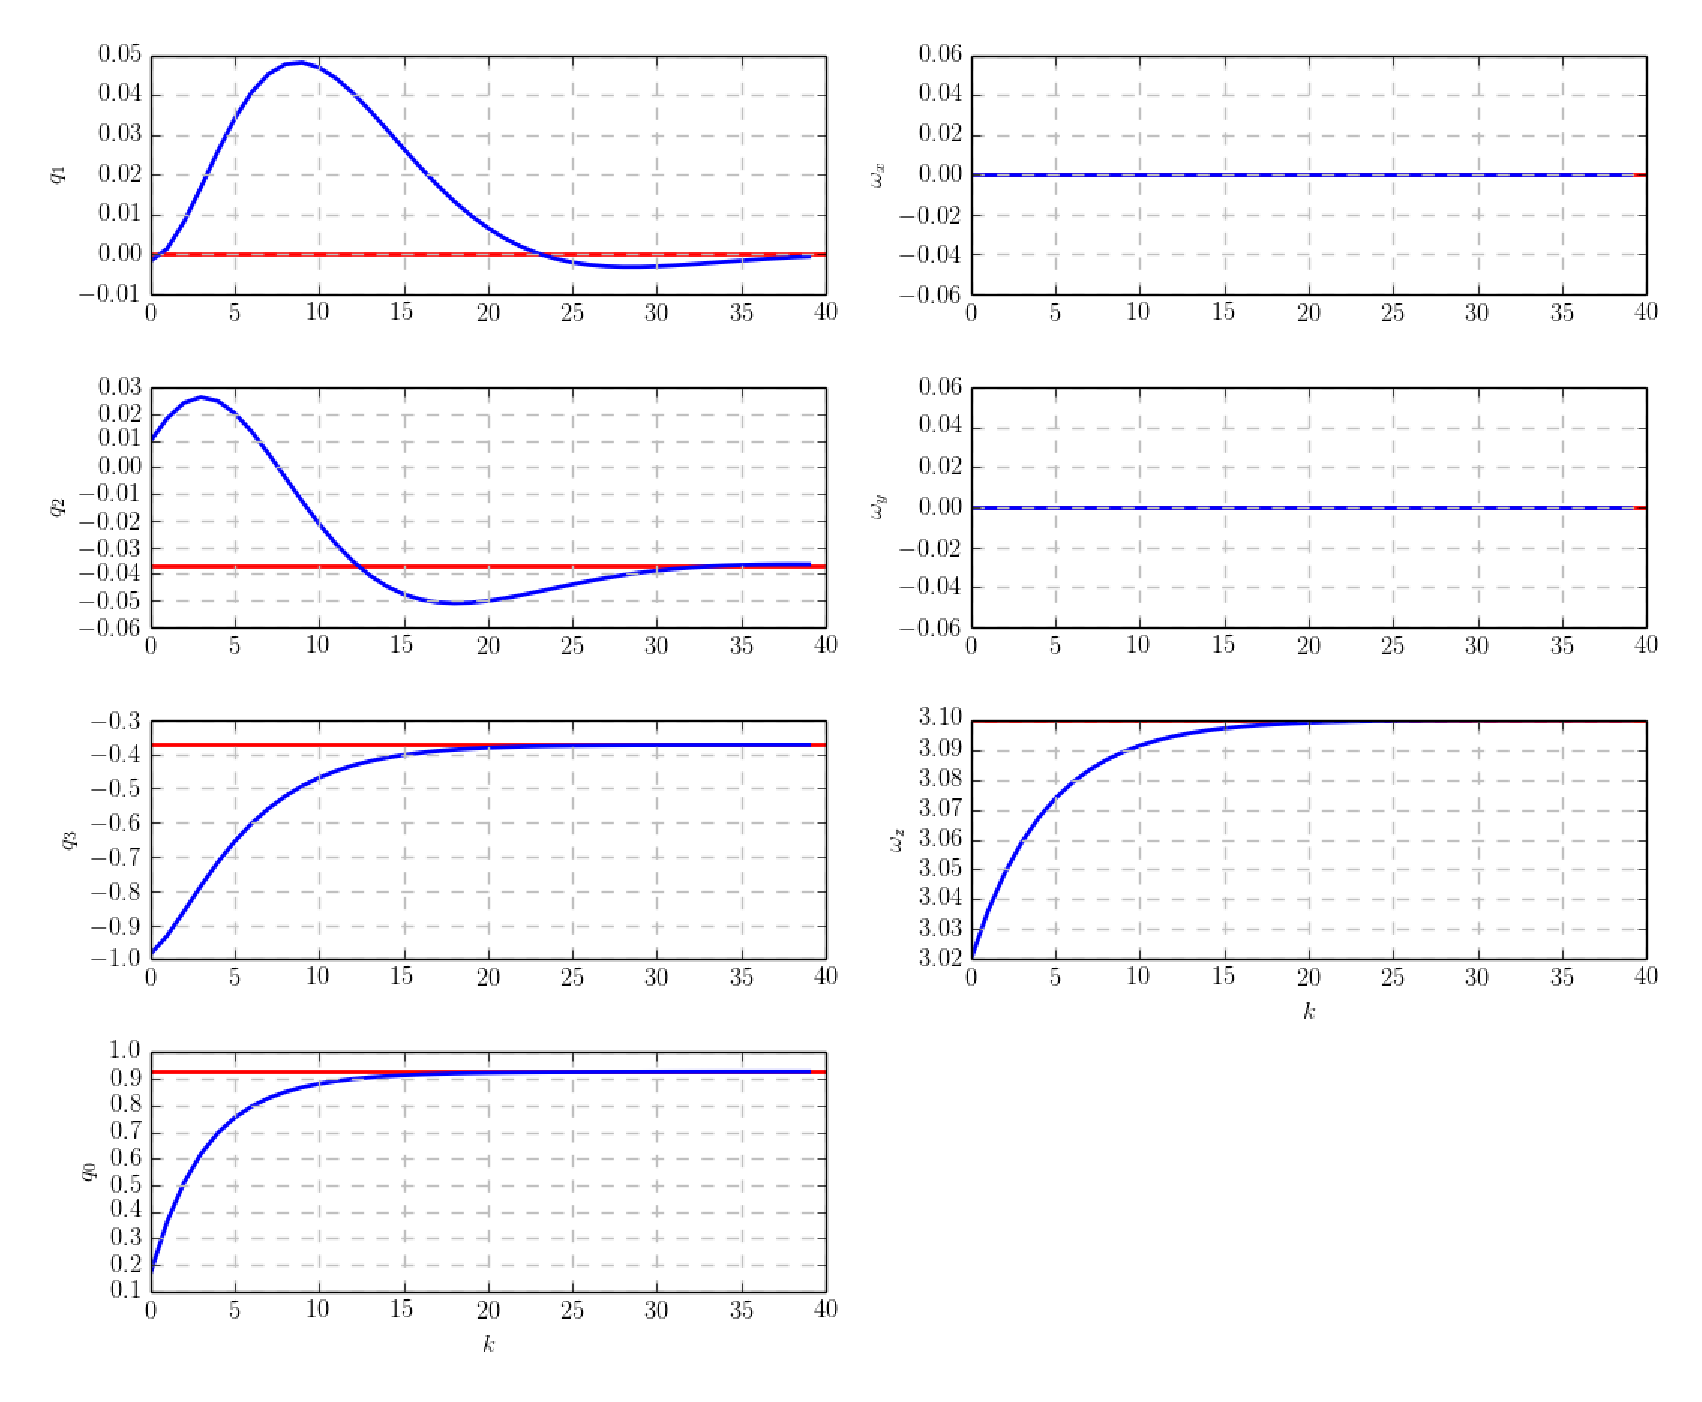
\psfig{file=figures/p_estimator_static_target.eps,width=6in}}
  \caption{P-Estimator with static target}
  \label{fig:PEstimatorwithstatictarget}
\end{figure}

The work covered so far in this chapter has all dealt with the a system in a static state.  In Figure \ref{fig:PEstimatorwithstatictarget}, a P-Estimator converges it's estimated state (blue) to the static measured state (red).  While the estimated state converges to the measured state after about 40 iterations, this type of conversion would be effective only for non-rotating systems.  The non-zero $\omega_z$ means that the quaternion attitude representation is in constant motion.

The $3.1$ rad/sec rotation about $0\bs{i} + 0.1\bs{j} + 1\bs{k}$ condition from the previous p-estimator is then allowed to propagate the quaternion state through 10 second of rotation with state estimate updates every 0.1 sec.  The resulting measured state (red) and estimated state (blue) is shown in Figure \ref{fig:PEstimatorwithrotatingtarget}.  The body rates track identically to those in Figure \ref{fig:PEstimatorwithstatictarget} where $t(k) = 2$ corresponds to $k = 20$.  Due to the proportional only compensation and no predictive methods, the initial transient behavior is followed by a behavior similar to a steady state error.

\begin{figure}[H]
  \centerline{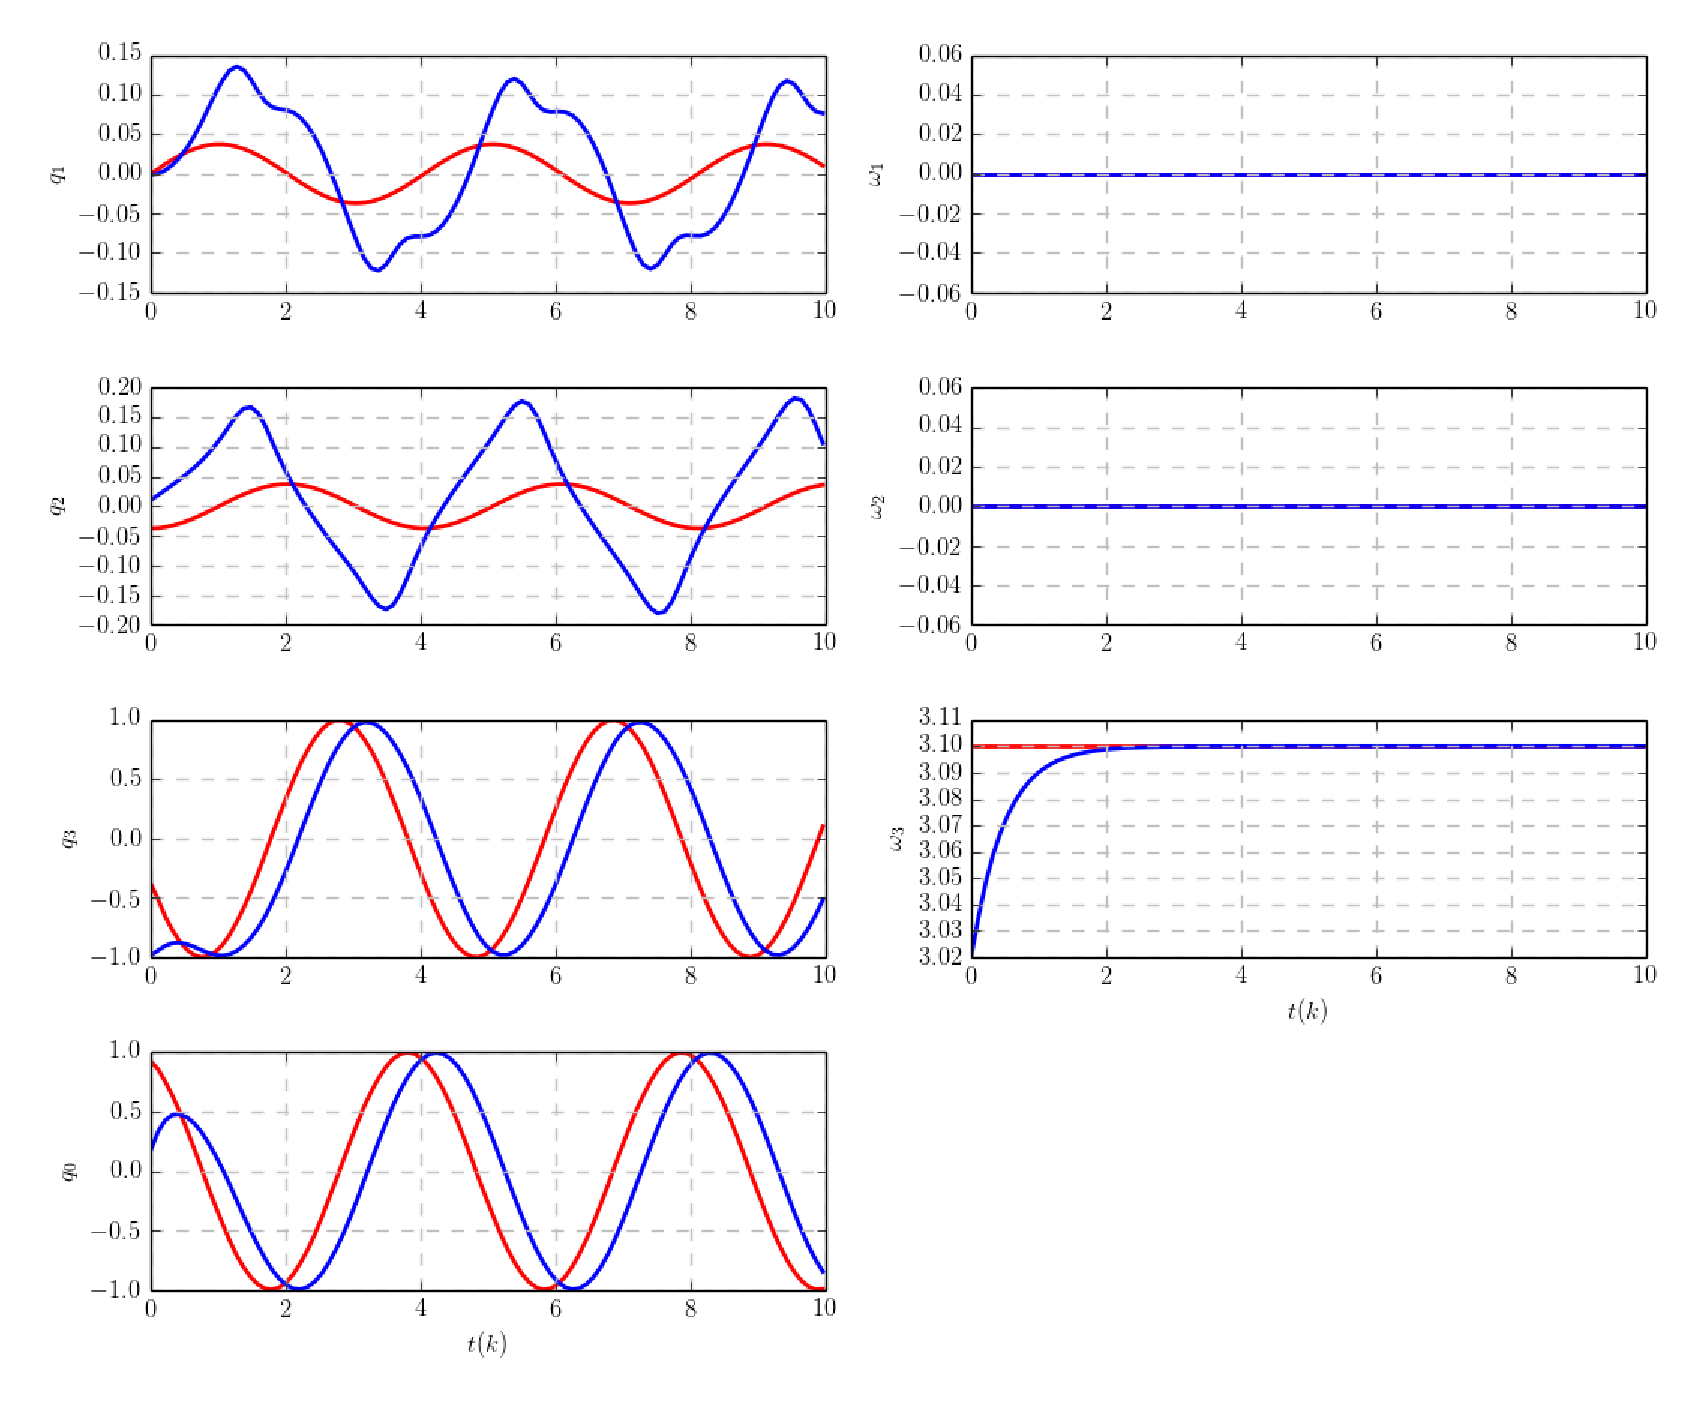
\psfig{file=figures/p_estimator_3radps.eps,width=6in}}
  \caption{P-Estimator with rotating target}
  \label{fig:PEstimatorwithrotatingtarget}
\end{figure}

Increasing the frequency of updates to the p-estimator can decrease the error between the measured and estimated states, but there is always be an error similar to a steady state error in the quaternion representation.  For better results the estimator needs to take into consideration changes in the state through the PID's integration and derivative terms.

\subsection{Integral State Estimation}
\label{subsec:IntegralEstimator}

To stay consistent with the findings in State Error (Chapter \ref{chap:StateError}), the quaternion portion of the integrated state should abide by the quaternion multiplicative correction method.  This is the first model where the variable sized time step is also taken into consideration.  Instead of accumulating the error measurements, the error corrections should be weighted according to the length of time between updates $t(k+1) - t(k)$.  In a simplified case the integral term should end up the same in the following two update instances.

\begin{table}[H]
  \centering
  \begin{tabular}{r|c|c|c|c|c}
    $t_1 (sec)$ & 0.1 & 0.2 & 0.3 & 0.4 & 0.5 \\ \hline
    $\theta_e$ & 4 & -3 & -3 & -3 & 5 \\
    \\
    $t_2 (sec)$ & 0.1 & & & 0.4 & 0.5 \\ \hline
    $\theta_e$ & 4 &  &  & -3 & 5 \\
  \end{tabular}
  \label{tbl:VariableUpdates}
\end{table}

In $t_1$, regular updates occur every 0.1 sec ending in an integral error value of 0.  In $t_2$, without taking into consideration the variable step sizes would end in an error value of $+6$, but really the -3 error update should be worth three times as much.

Running the state estimator without compensating for variations in time step sizes can create inconsistencies between different experimental runs.  In Figure \ref{fig:IEstimatorwithouttimevariationcompensation}, the integral estimator was updated with a fixed state for 30 seconds.  The estimator was initialized at $0$ radians and run three times against a fixed angle of $0.5$ radians.  The first time with an estimation update frequency of every 0.4 seconds (blue), second with the update frequency of every 0.1 seconds (red), and third with a variable update frequency (green) that jumped back and forth between updating every 0.05 and 0.4 seconds.

\begin{figure}[H]
  \centerline{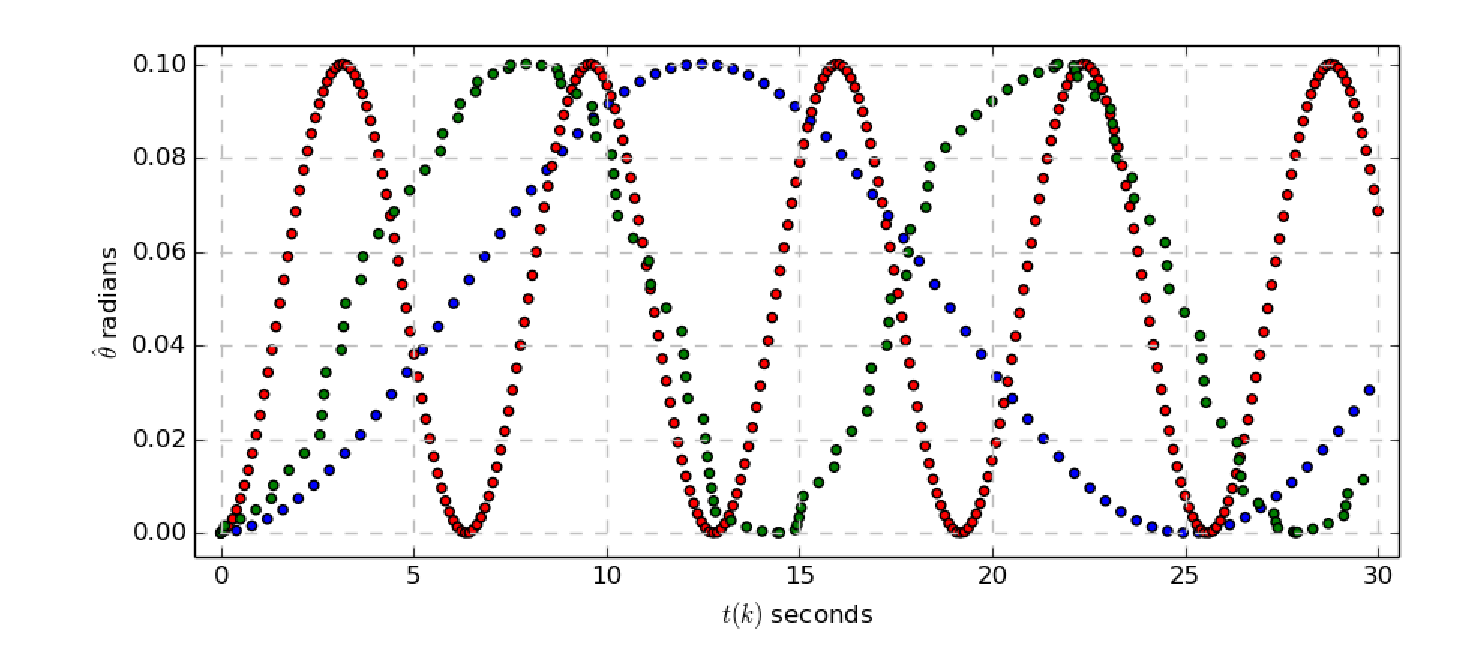
\psfig{file=figures/i_estimator_no_time_varying.eps,width=6in}}
  \caption{I-Estimator without time variation compensation}
  \label{fig:IEstimatorwithouttimevariationcompensation}
\end{figure}

Each calculated estimate for $\hat{\theta}$ in the $k$ domain is identical for each of the three runs, but varies greatly in the time domain.  Most notably, the third run that alternates between update frequencies ends up creating an estimation dynamic that could make the controller less robust.

In comparison, the PID estimator was modified to incorporate the time step size into it's integral term.  The same three tests were run as above with the 0.1 (red), 0.4 (blue), and variable 0.05/0.4 (green) time steps.  The adjustment quaternion method from Section \ref{sec:HighIntegrityStateAdjustments} is first used to compensate for measured time step size of $\Delta t_{k}$ creating a consistent error quaternion. then is used as before to scale the error quaternion by the selected gain value.  The results of this work can be seen in Figure \ref{fig:IEstimatorwithtimevariationcompensation} where the three test runs are still not identical, but their dynamics are more similar than before.  More notably, the variable step test (green) shows less variability in the estimate being produced which will reduce the noise being transferred to the control algorithm.

\begin{equation}
  \begin{aligned}
    \bs{\hat{x}}(t_{k+1}) &= \begin{bmatrix} \bs{\hat{q}}(t_{k+1}) \\ \bs{\hat{\omega}}(t_{k+1}) \end{bmatrix} =
    \begin{bmatrix} \bs{\psi}\big(\bs{q}_{ei}(t_k), K_{qi}\big) \otimes \bs{\hat{q}}(t_{k}) \\
     \bs{\hat{\omega}}(t_{k}) + \bs{K}_{\omega i} \cdot (\Delta t_k \bs{I})\cdot \bs{\omega}_e(t_{k}) \end{bmatrix} \\
    \text{where }\bs{q}_{ei}(t_k) &= \bs{\psi}(\bs{q}_e(t_{k}), \Delta t_{k}) \otimes \bs{q}_{ei}(t_{k-1})
  \end{aligned}
  \label{eqn:IEstimator}
\end{equation}

In Equation \ref{eqn:IEstimator}, the error quaternion $\bs{q}_{ei}(t_k)$ used is an accumulation of the time step scaled errors encountered in all previous steps.  This is analogous to a running summation of the error values.  For the body rate estimation, it's largely the traditional integral component with an extra $\Delta t_k \bs{I}$ term that linearly scales the body rate error calculations based on the size of the current time step.

\begin{figure}[H]
  \centerline{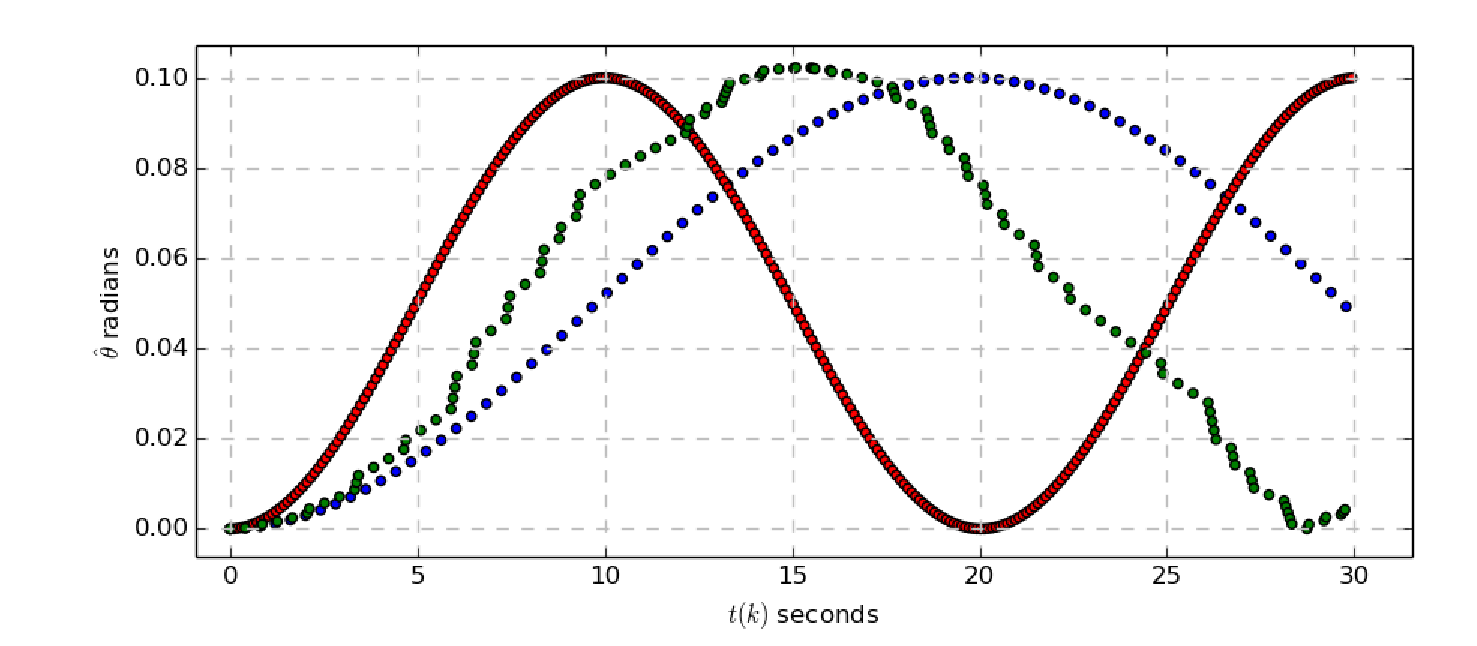
\psfig{file=figures/i_estimator_time_varying.eps,width=6in}}
  \caption{I-Estimator with time variation compensation}
  \label{fig:IEstimatorwithtimevariationcompensation}
\end{figure}

\subsection{Derivative State Estimation}
\label{subsec:DerivativeEstimator}

The derivative component of the PID estimator takes a similar form to the integral component in Equation \ref{eqn:IEstimator}.  The derivative component is only concerned with the current error, previous error, and the current time step size.  As with the integral body rate correction, the derivative correction is scaled by $\frac{1}{\Delta t_k}$ to compensate for variable step sizes.

\begin{equation}
  \begin{aligned}
    \bs{\hat{x}}(t_{k+1}) &= \begin{bmatrix} \bs{\hat{q}}(t_{k+1}) \\ \bs{\hat{\omega}}(t_{k+1}) \end{bmatrix} =
    \begin{bmatrix} \bs{\psi}\left(\bs{q}_{ed}(t_k), K_{qd}\right) \otimes \bs{\hat{q}}(t_{k}) \\
     \bs{\hat{\omega}}(t_{k}) + \bs{K}_{\omega d} \cdot \left(\frac{1}{\Delta t_k} \bs{I}\right) \cdot \bs{\omega}_e(t_{k}) \end{bmatrix} \\
    \text{where } \bs{q}_{ed}(t_k) &= \bs{\psi}\left(\bs{q}_e(t_{k-1})^* \otimes \bs{q}_e(t_{k}), \frac{1}{\Delta t_{k}}\right)
  \end{aligned}
  \label{eqn:DEstimator}
\end{equation}

The Figures \ref{fig:DEstimatorwithouttimevariationcompensation} and \ref{fig:DEstimatorwithtimevariationcompensation} below are the results of three test runs with the same set up update frequencies as with the integral component (0.1/sec, 0.4/sec, and varied).  For this comparison, the TableSat was simulated into a steady $0.01$ rad/s rotation about the body $+z$-axis to generate a constant rate of change for the quaternion instead of the fixed quaternion in the integral test.  The $\theta_{adj}$ parameter tracked for this test is the angular rotation associated with the $\bs{\psi}\left(\bs{q}_{ed}(t_k), K_{qd}\right)$ quaternion adjustment term.

\begin{figure}[H]
  \centerline{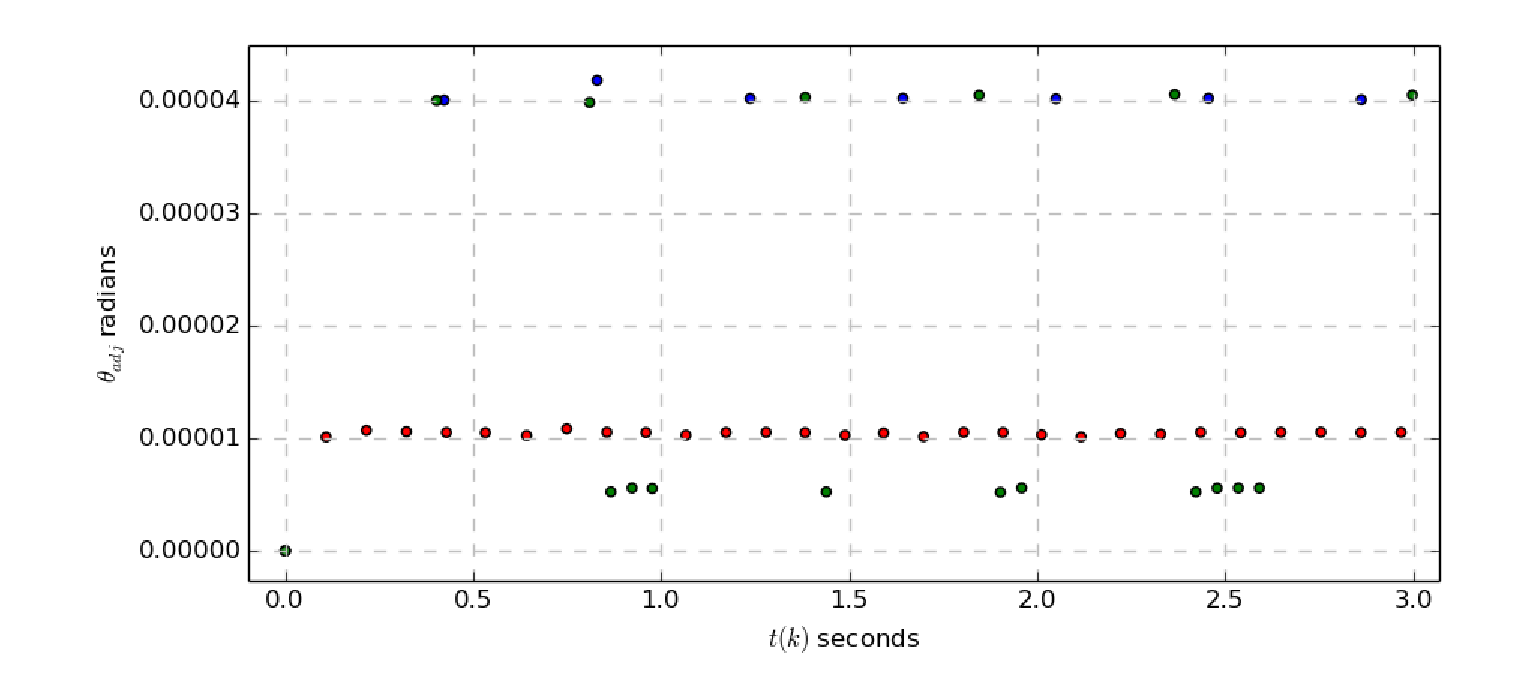
\psfig{file=figures/d_estimator_no_time_varying.eps,width=6in}}
  \caption{D-Estimator without time variation compensation}
  \label{fig:DEstimatorwithouttimevariationcompensation}
\end{figure}

Figure \ref{fig:DEstimatorwithouttimevariationcompensation} shows the results of the test run without consideration taken for time step sizes.  With a constant spin rate, the resulting quaternion adjustment is tightly coupled to the frequency that the updates are made with the 0.1 (red), 0.4 (blue), and variable 0.05/0.4 (green) time steps.  The variable time step sequence is a particular concerns as it jumps back and forth between adjusted amount suggesting the spin rate is not constant.

\begin{figure}[H]
  \centerline{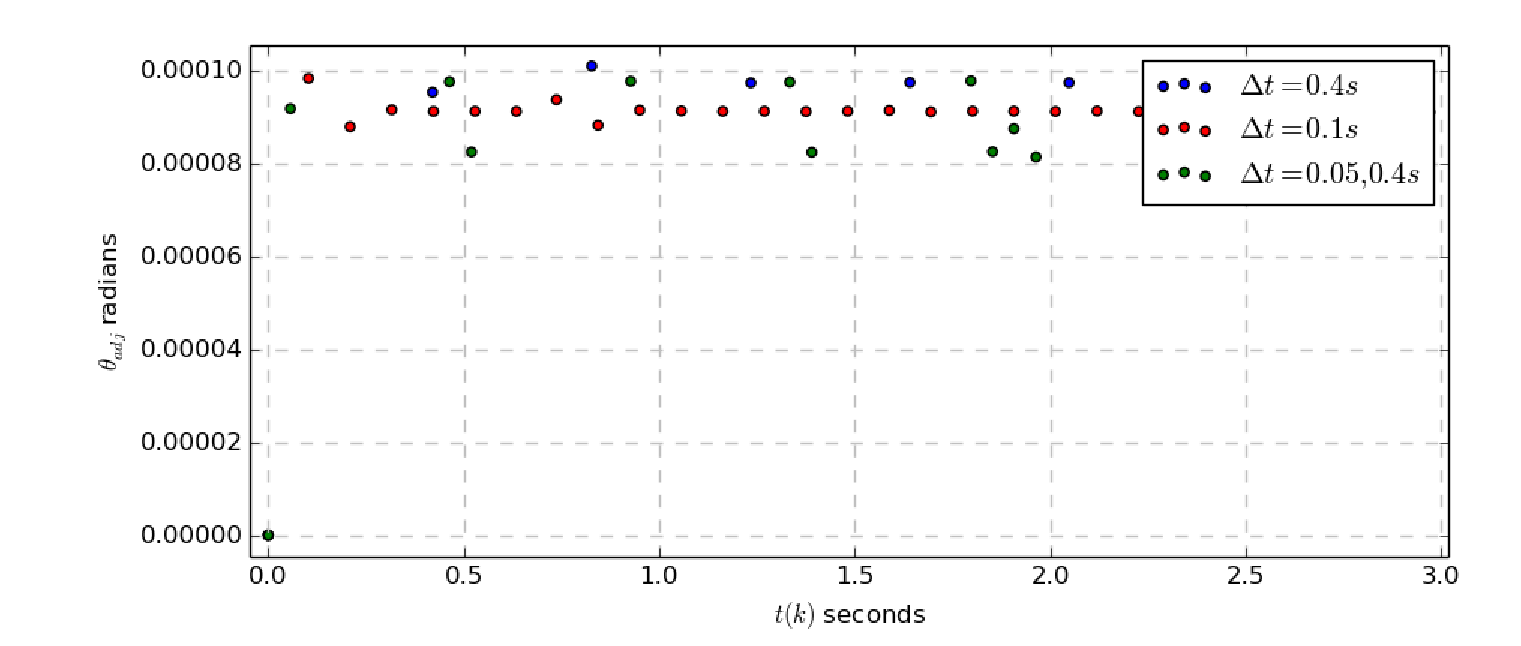
\psfig{file=figures/d_estimator_time_varying.eps,width=6in}}
  \caption{D-Estimator with time variation compensation}
  \label{fig:DEstimatorwithtimevariationcompensation}
\end{figure}

Figure \ref{fig:DEstimatorwithtimevariationcompensation} implements the time variation compensation in Equation \ref{eqn:DEstimator} where the quaternion adjustments provide a better representation of the measured constant spin rate.

\subsection{PID State Estimation of Unforced Motion}
\label{subsec:PIDEstimatorofUnforcedMotion}

Combining the proportional, integral, and derivative estimator portions from above.  Equations \ref{eqn:PEstimator}, \ref{eqn:IEstimator}, and \ref{eqn:DEstimator} get combined into a single PID estimator as

\begin{equation}
  \bs{\hat{x}}(t_{k+1}) = \begin{bmatrix} \bs{\psi}\left(\bs{q}_{ed}(t_k), K_{qd}\right) \otimes \bs{\psi}\big(\bs{q}_{ei}(t_k), K_{qi}\big) \otimes \bs{\psi}(\bs{q}_e(t_{k}), K_{qp})  \otimes \bs{\hat{q}}(t_{k}) \\
  \bs{\hat{\omega}}(t_{k}) + \bs{K}_{\omega p} \cdot \bs{\omega}_e(t_{k}) + \bs{K}_{\omega i} \cdot (\Delta t_k \bs{I})\cdot \bs{\omega}_e(t_{k}) + \bs{K}_{\omega d} \cdot \left(\frac{1}{\Delta t_k} \bs{I}\right) \cdot \bs{\omega}_e(t_{k}) \end{bmatrix}
  \label{eqn:PIDEstimatorUnforcedMotion}
\end{equation}

The update to the estimated body rate follows the traditional method of the PID control with the addition of the scaling factors for the integral and derivative terms that compensate for non-uniform step sizes at run-time.  The quaternion correction is a compilation of the individual correction quaternions and joined through the multiplicative error correction method.

With a spin-stabilized system controlling the body rate is relatively straight forward with a PID controller.  A test was run through TSatPy with based on the PID estimation in Equation \ref{eqn:PIDEstimatorUnforcedMotion}.  The system was set at a spin rate of $0.314$ rad/sec rotation about $+z$ with the measurement of the quaternion angle $\theta$ containing noise $N \sim (0, 0.1218)$ radians.  A gradient descent gain selection settled on the following parameters.

\begin{equation}
  \begin{aligned}
    K_{qp} &= 0.98, K_{qi} = 0.001, K_{qd} = 0.001 \\
    \bs{K}_{\omega p} &= 0.7 \bs{I}, \bs{K}_{\omega i} = \bs{0}, \bs{K}_{\omega d} = \bs{0}
  \end{aligned}
\end{equation}

The test run results are show in Figure \ref{fig:PIDEstimatorwithoutstateprediction}.  The bottom two graphs showing body rate tracking performance where the basic proportional control quickly brings the body rate error under control.  The quaternion estimations are much more difficult largely due to the lack of a system model to convert body rates to estimated attitudes at the next update.  Since the system is spin-stabilized and the estimated quaternion has no prior knowledge of where the next value will be, it relies on a large proportional component to jump to the new measurement values on each update.

While testing the performance of the integral and derivative components showed an improved performance when incorporating the effects of the variable time step, in this test with such a heavy reliance on the proportional component, the benefits to considering the variable time step effects were negligible.

\begin{figure}[H]
  \centerline{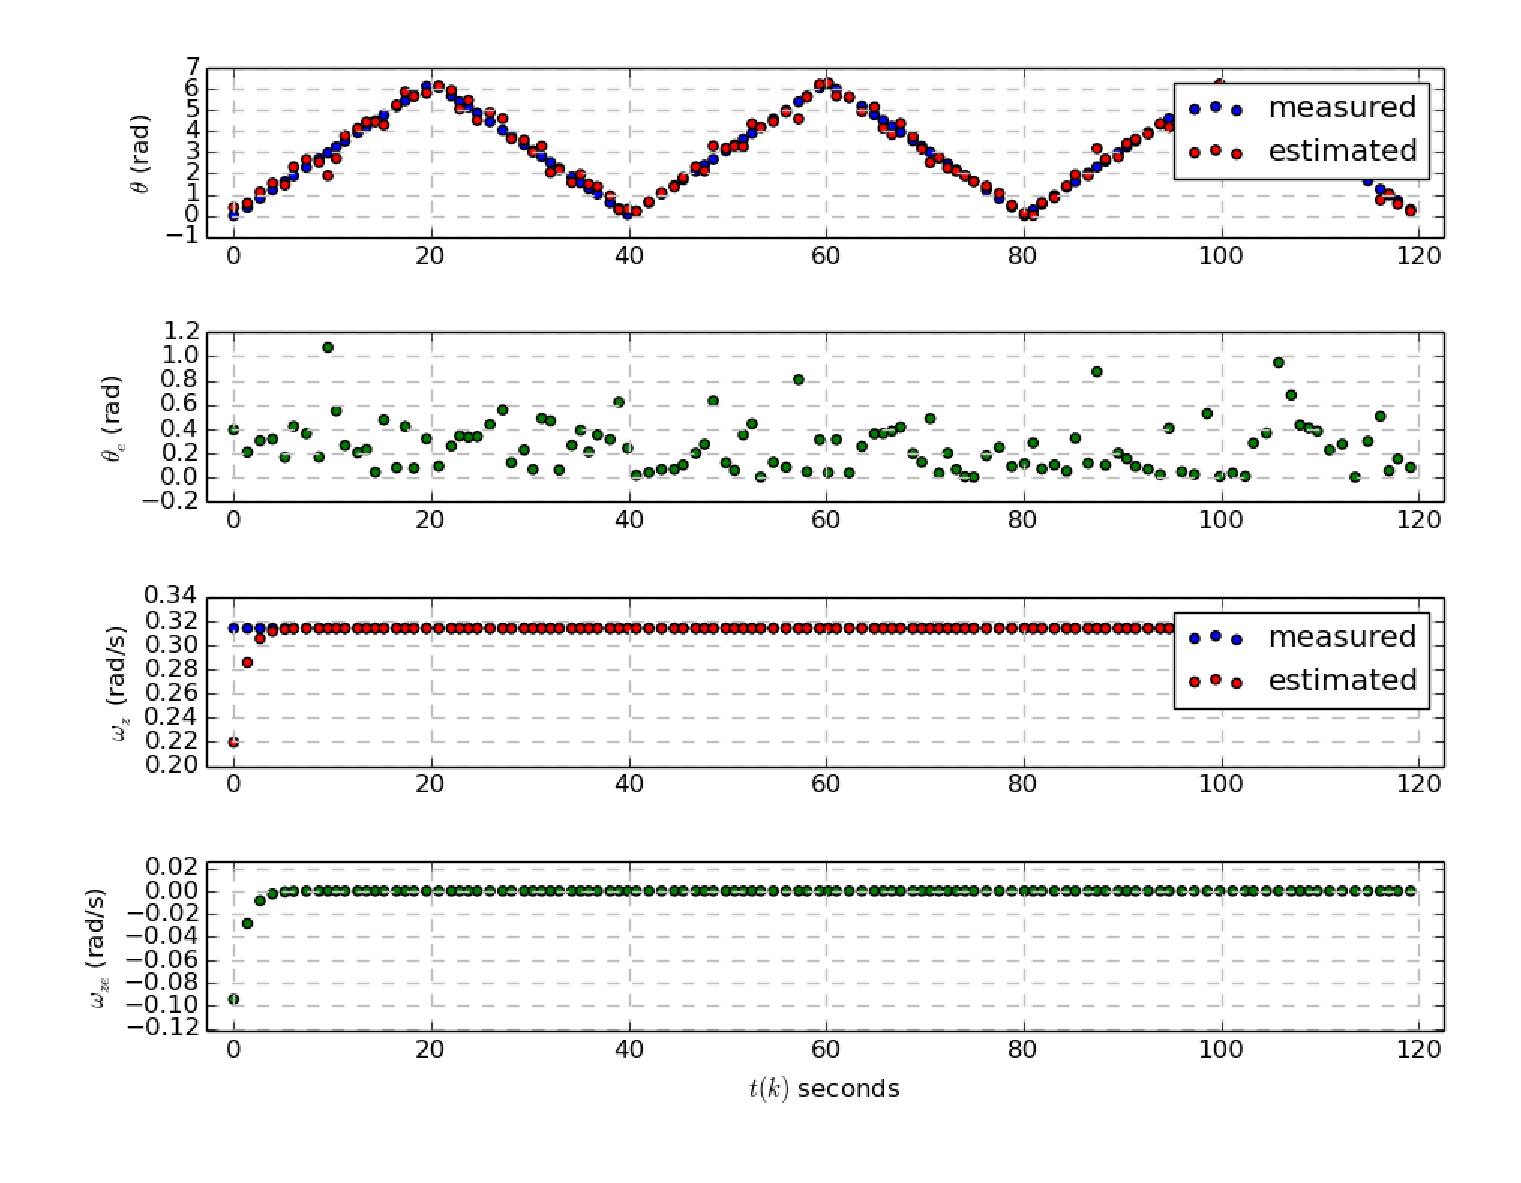
\psfig{file=figures/pid_estimator_no_prediction_high_P.eps,width=6in}}
  \caption{PID-Estimator without state prediction}
  \label{fig:PIDEstimatorwithoutstateprediction}
\end{figure}


\subsection{PID Estimation with State Prediction}
\label{subsec:PIDEstimatorwithStatePrediction}

From Section \ref{sec:BodyRatePIDEstimation}, Equation \ref{eqn:PIDEstimatorUnforcedMotion} defines a method of tracking unforced spin-stabilized satellites through PID state estimation.  The biggest issue was a heavy reliance on the proportional gain to track the quaternion attitude which is sensitive to measurement noise.  Incorporating a multiplicative-correction quaternion based model of rigid body dynamics based on the equations in Chapter \ref{chap:SatelliteAttitudeDynamicsAndKinematics} can assist in predicting the $t_{k+1}$ state of the system.

\begin{equation}
  \bs{\hat{x}}(t_{k+1}) = \begin{bmatrix} \bs{\psi}\left(\bs{q}_{ed}(t_k), K_{qd}\right) \otimes \bs{\psi}\big(\bs{q}_{ei}(t_k), K_{qi}\big) \otimes \bs{\psi}(\bs{q}_e(t_{k}), K_{qp})  \otimes \bs{\hat{q}}(t_{k+1})^- \\
  \bs{\hat{\omega}}(t_{k+1})^- + \bs{K}_{\omega p} \cdot \bs{\omega}_e(t_{k}) + \bs{K}_{\omega i} \cdot (\Delta t_k \bs{I})\cdot \bs{\omega}_e(t_{k}) + \bs{K}_{\omega d} \cdot \left(\frac{1}{\Delta t_k} \bs{I}\right) \cdot \bs{\omega}_e(t_{k}) \end{bmatrix}
  \label{eqn:PIDEstimatorwithPredictionUnforcedMotion}
\end{equation}

with the a priori state $\bs{\hat{x}}(t_{k+1})^-$ as

\begin{equation}
  \bs{\hat{x}}(t_{k+1})^- = \begin{bmatrix}\bs{\hat{q}}(t_{k+1})^- \\ \bs{\hat{\omega}}(t_{k+1})^- \end{bmatrix} = f \Big( \bs{\hat{q}}(t_{k}), \bs{\hat{\omega}}(t_{k}) \Big)
\end{equation}

The PID estimator now with a state prediction method was run under the same testing conditions present in Figure \ref{fig:PIDEstimatorwithoutstateprediction}.  The resulting performance showed that the inclusion of the system model greatly reduced the reliance on the proportional component of the PID estimator which reduced the noise and increased the accuracy of the final estimates being provided to the controller.  The results in Figure \ref{fig:PIDEstimatorwithstateprediction} show the improved quaternion angle estimates when run with the following gains.

\begin{equation}
  \begin{aligned}
    K_{qp} &= 0.0735, K_{qi} = 0.000863, K_{qd} = 0.00812 \\
    \bs{K}_{\omega p} &= 0.7 \bs{I}, \bs{K}_{\omega i} = \bs{0}, \bs{K}_{\omega d} = \bs{0}
  \end{aligned}
\end{equation}

The quaternion's proportional value is still the dominant gain, but has been reduced by 92.5\% of it's previous value while still providing about 80\% reduction in quaternion attitude error rates.

\begin{figure}[H]
  \centerline{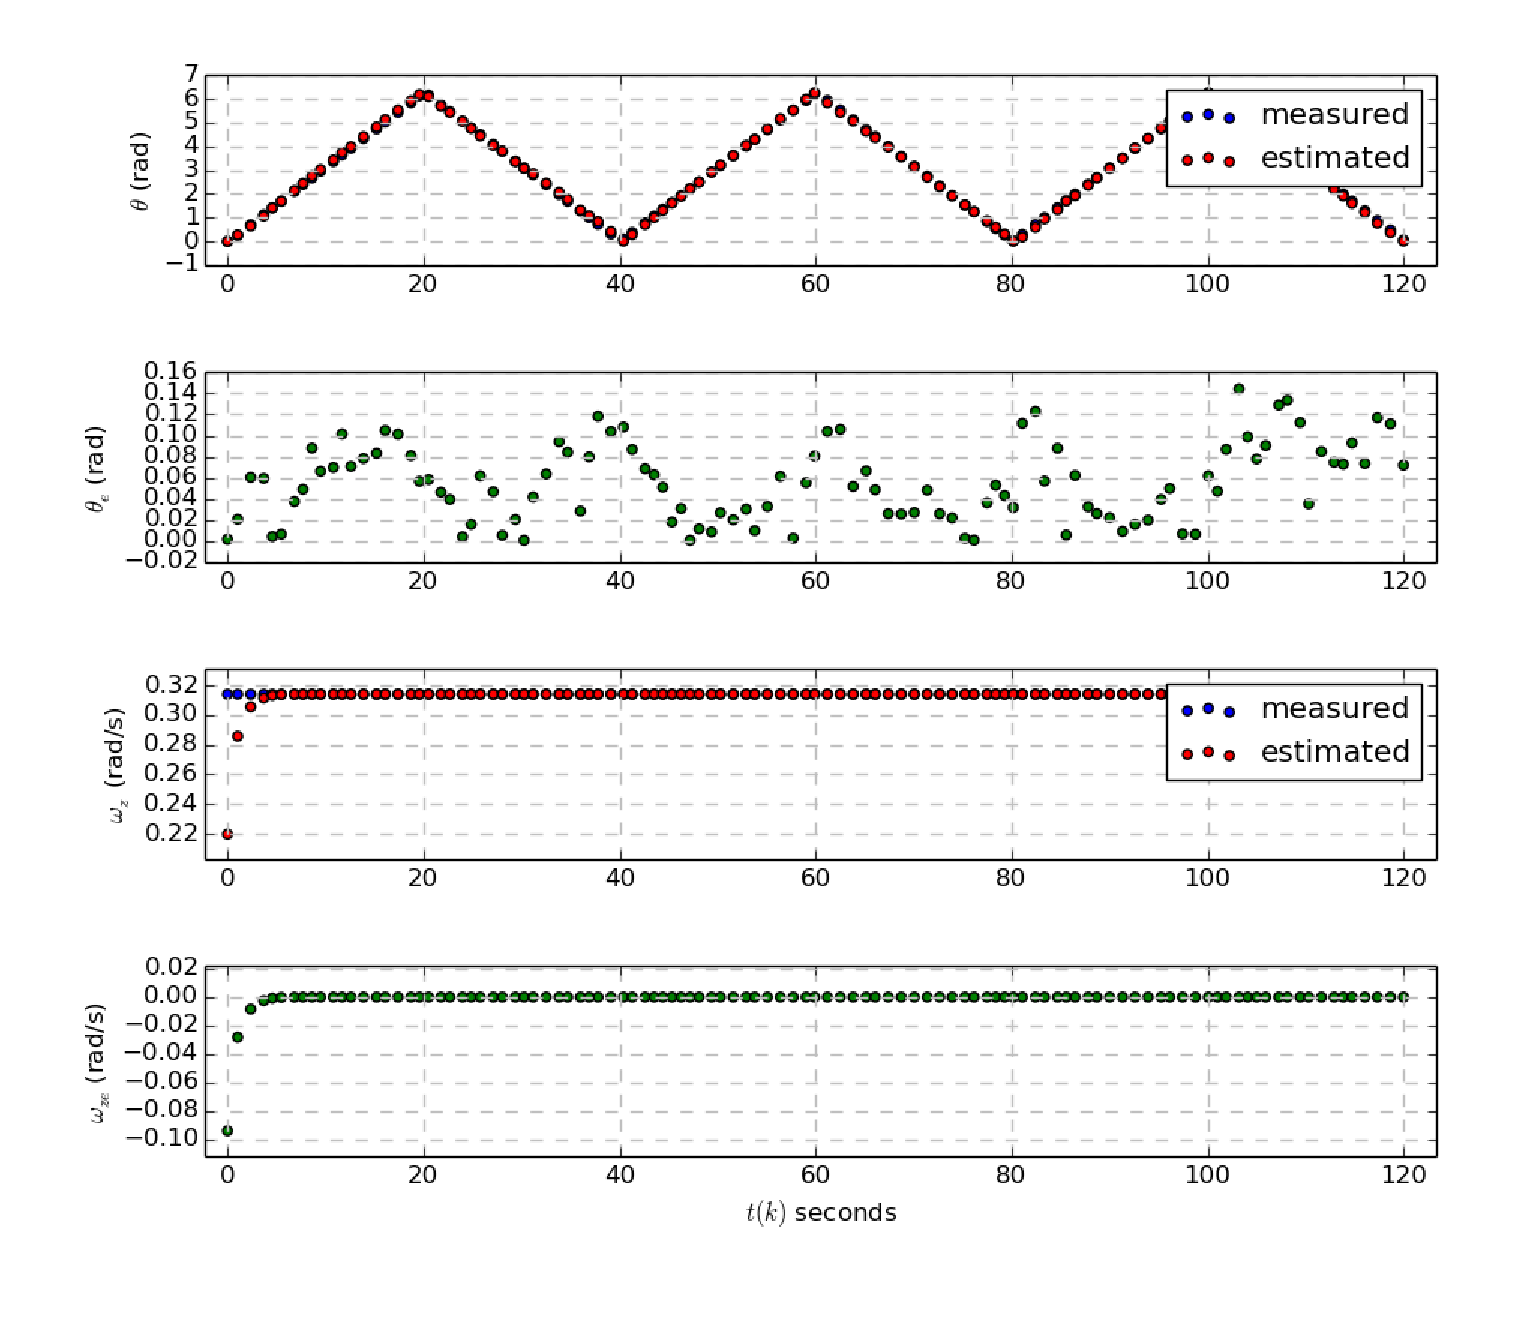
\psfig{file=figures/pid_estimator_with_prediction.eps,width=6in}}
  \caption{PID-Estimator with state prediction}
  \label{fig:PIDEstimatorwithstateprediction}
\end{figure}


\section{Sliding Mode Observer with State Prediction}
\label{sec:SlidingModeObserverwithStatePrediction}

The Sliding Mode Observer (SMO) is a proportional estimator with an additional smoothing term that uses a chosen sliding surface.  The general form for the SMO is

\begin{equation}
  \bs{\dot{\hat{x}}} = \bs{\hat{f}}(\bs{\hat{x}}, \bs{\hat{u}}, t) + \bs{L}(\bs{C}\bs{\hat{x}} - \bs{C}\bs{x}) + \bs{K}\bs{1}_s\bs{\hat{y}}
  \label{eqn:SMOContinuous}
\end{equation}

\begin{figure}[ht]
  \centerline{
\psfig{file=figures/saturation_function.eps,height=1in}}
  \caption{Saturation Function}
  \label{fig:SaturationFunction}
\end{figure}


Where L is a luenberger gain and $\bs{1}_s$ is a switching function based on $s$.  The sliding mode terms allow additional control of the state adjustments without adding a lot of computational complexity.  The SMO can continue to use the nonlinear model's state predictions as in the PID estimators in Section \ref{subsec:PIDEstimatorwithStatePrediction}, which is an advantage over methods such as the Extended Kalman Filter (EKF) where the system is linearized about an operating point and assumes a constant time step.

This thesis takes the discretized form of Equation \ref{eqn:SMOContinuous} with a quaternion multiplicative correction

\begin{equation}
  \bs{\hat{x}}(t_{k+1}) = \begin{bmatrix} \bs{\psi} (\bs{1}_s\big(\bs{q}_{e}(t_k)\big), K_q) \otimes \bs{\psi}(\bs{q}_e(t_{k}), L_{q})  \otimes \bs{\hat{q}}(t_{k+1})^- \\
  \bs{\hat{\omega}}(t_{k+1})^- + \bs{L}_{\omega} \bs{\omega}_e(t_{k}) + \bs{K}_{\omega}\bs{1}_s \big(\bs{\omega}_e(t_{k}) \big) \end{bmatrix}
  \label{eqn:SMOEstimatorwithPredictionUnforcedMotion}
\end{equation}

where

\begin{subequations}
  \begin{align}
    \bs{1}_s\big(\bs{q}_{e}(t_k) \big) &= \begin{bmatrix} \bs{v_e} \\ sat\left( \frac{2\cos^{-1} q_{0e} }{S_{q}} \right) \end{bmatrix} \\
    \bs{1}_s \big(\bs{\omega}_e(t_{k}) \big) &= sat\left( \frac{\bs{\omega}_e(t_{k})}{S_{\omega}} \right) \\
    \bs{L}_{\omega} &= L_\omega \cdot \bs{I} \\
    \bs{K}_{\omega} &= K_\omega \cdot \bs{I}
  \end{align}
\end{subequations}

For body rates, the a priori state provides the predicted body rate $\bs{\hat{\omega}}(t_{k+1})^-$ that gets adjusted by a proportional term $\bs{L}_{\omega} \bs{\omega}_e(t_{k})$ as in the P-Estimator, but has an additional saturation function correction based on sliding surfaces for the individual body rate errors.  As found in the PID estimator, the proportional estimator for a steady spin-stabilized satellite performs adequately.

Similar to the PID estimator, the quaternion sliding mode observer limits it's focus to the angular measure of the rotational quaternion.  The sliding surface is taken based on the radian measure.  If the radian measure is below the saturation limit, the quaternion stays as is.  If the quaternion represents a rotation greater than the saturation limit a saturated quaternion is created about the same Euler axis but limit to the saturation angle of rotation.

Running the same tests as run against the PID estimators, the following parameters were located through an iterative gradient descent method that minimized the quaternion error angle and standard deviation of the error angle.

\begin{equation}
  \begin{aligned}
    L_q = 0.282 &, L_w = 0.444 \\
    K_q = 0.307 &, K_w = 0.464 \\
    S_q = 0.886 &, S_w = 0.569 \\
  \end{aligned}
\end{equation}

Figure \ref{fig:SMOEstimatorwithstateprediction} shows the result of the test at these optimized parameters.  The inverted angle measurement in the first graph is an artifact of the non-unique representation of a quaternion attitude.  In this case, the estimated angles are being calculated for rotations about the body's $-z$-axis instead of the $+z$ axis.  This further supports the decision made in Section \ref{chap:StateError} to use the multiplicative error as the second graph shows the correct error values.

Although the SMO in this case is able to traverse the initial transient response well, the steady state quaternion error is almost as high as using a PID estimator with no state prediction method.  This behavior is due to the high quaternion measurement noise.  With the saturation function, the sliding mode observer is still largely a proportional estimator without the assistance of an integral term to smooth out the noise.

\begin{figure}[H]
  \centerline{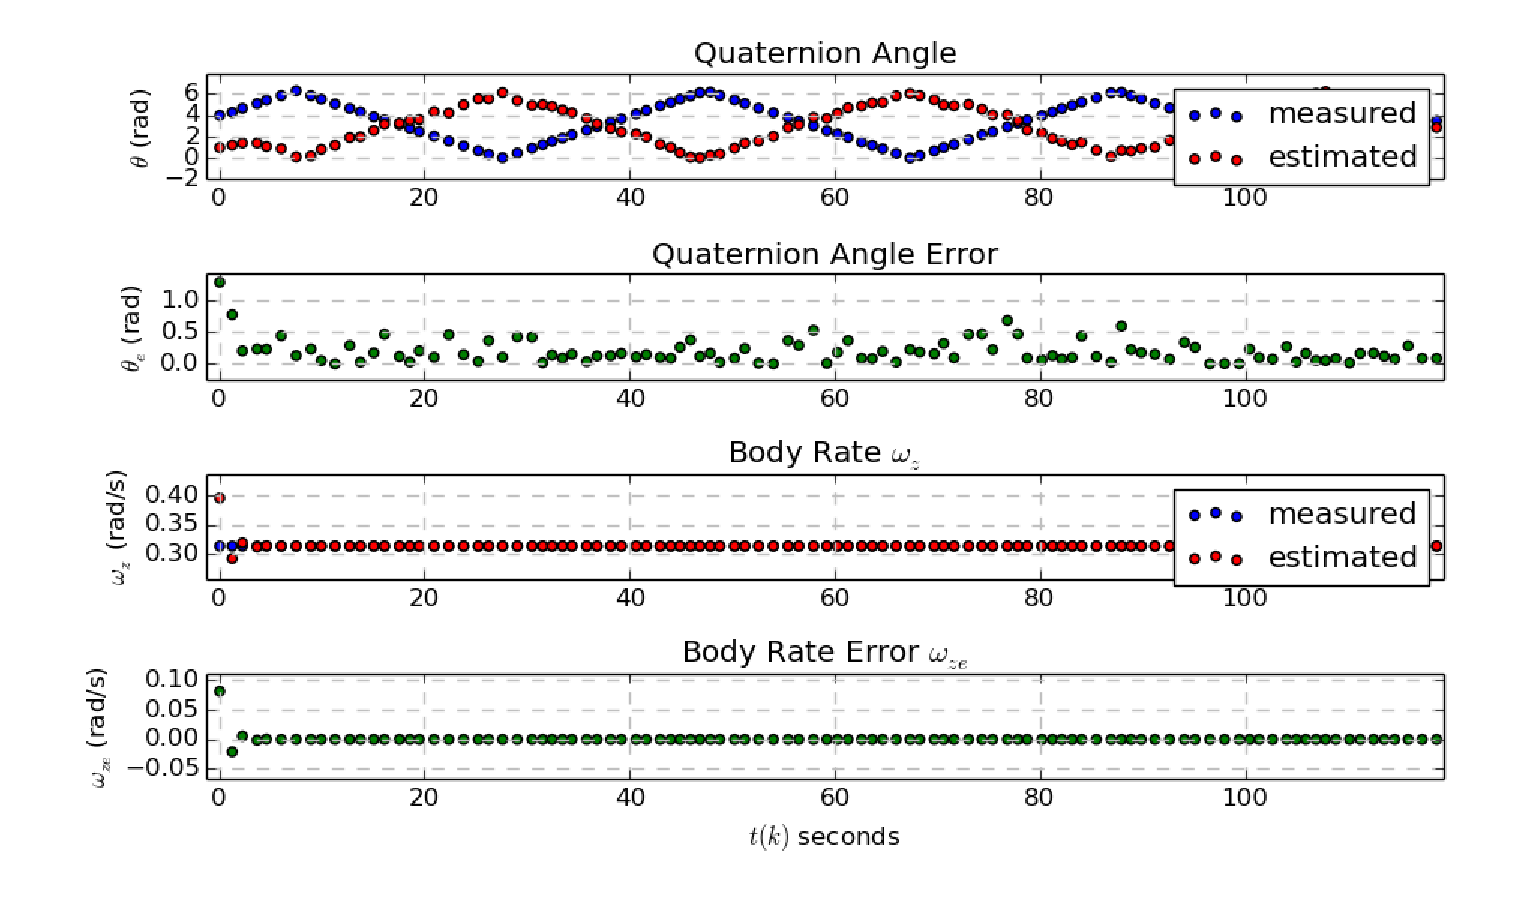
\psfig{file=figures/smo_estimator_with_prediction.eps,width=6in}}
  \caption{SMO-Estimator with state prediction}
  \label{fig:SMOEstimatorwithstateprediction}
\end{figure}

Based on these results, the SMO performs acceptably for the body rate estimation, but according to the steady state error rates, it appears that the PID estimation would be a better use for the steady state attitude tracking.  Both estimators have similar performance profiles which makes it more complicated to determine the better choice.  Section \ref{sec:ComparativeAnalysysofPIDandSMOEstimators} will go over how TSatPy can assist with running both estimation techniques in parallel for to provide a more accurate representation.

\section{Comparative Analysis of PID and SMO Estimators}
\label{sec:ComparativeAnalysysofPIDandSMOEstimators}

One of the advantages to developing the TSatPy code base for the TableSat spin-stabilized is the ability to run a comparative analysis of multiple estimators at the same time.  The estimators run agnostic to the source of the measurements.  In the sample shown below, the state measurements were generated by a model, but could also be switched to be pulled off the TableSat.

Figure \ref{fig:PIDSMOEstimatorConcurrentComparison} was generated by running a single simulation an providing the truth model's measured state to both a PID and SMO estimator tuned to the parameters selected during individual gain tuning tests above.  This allows for a clear side-by-side comparison of their performance.  Multiple runs all have similar characteristics.  In the initial transient response both estimators are able to converge to a steady state after just a couple updates, but the SMO is able to converge slightly faster each time.  For the steady state response the PID estimator consistently maintains a lower average error, although with a slightly higher standard deviation.  As with the initial response, the SMO estimation values generally update slightly just before the PID estimator.

\begin{figure}[H]
  \centerline{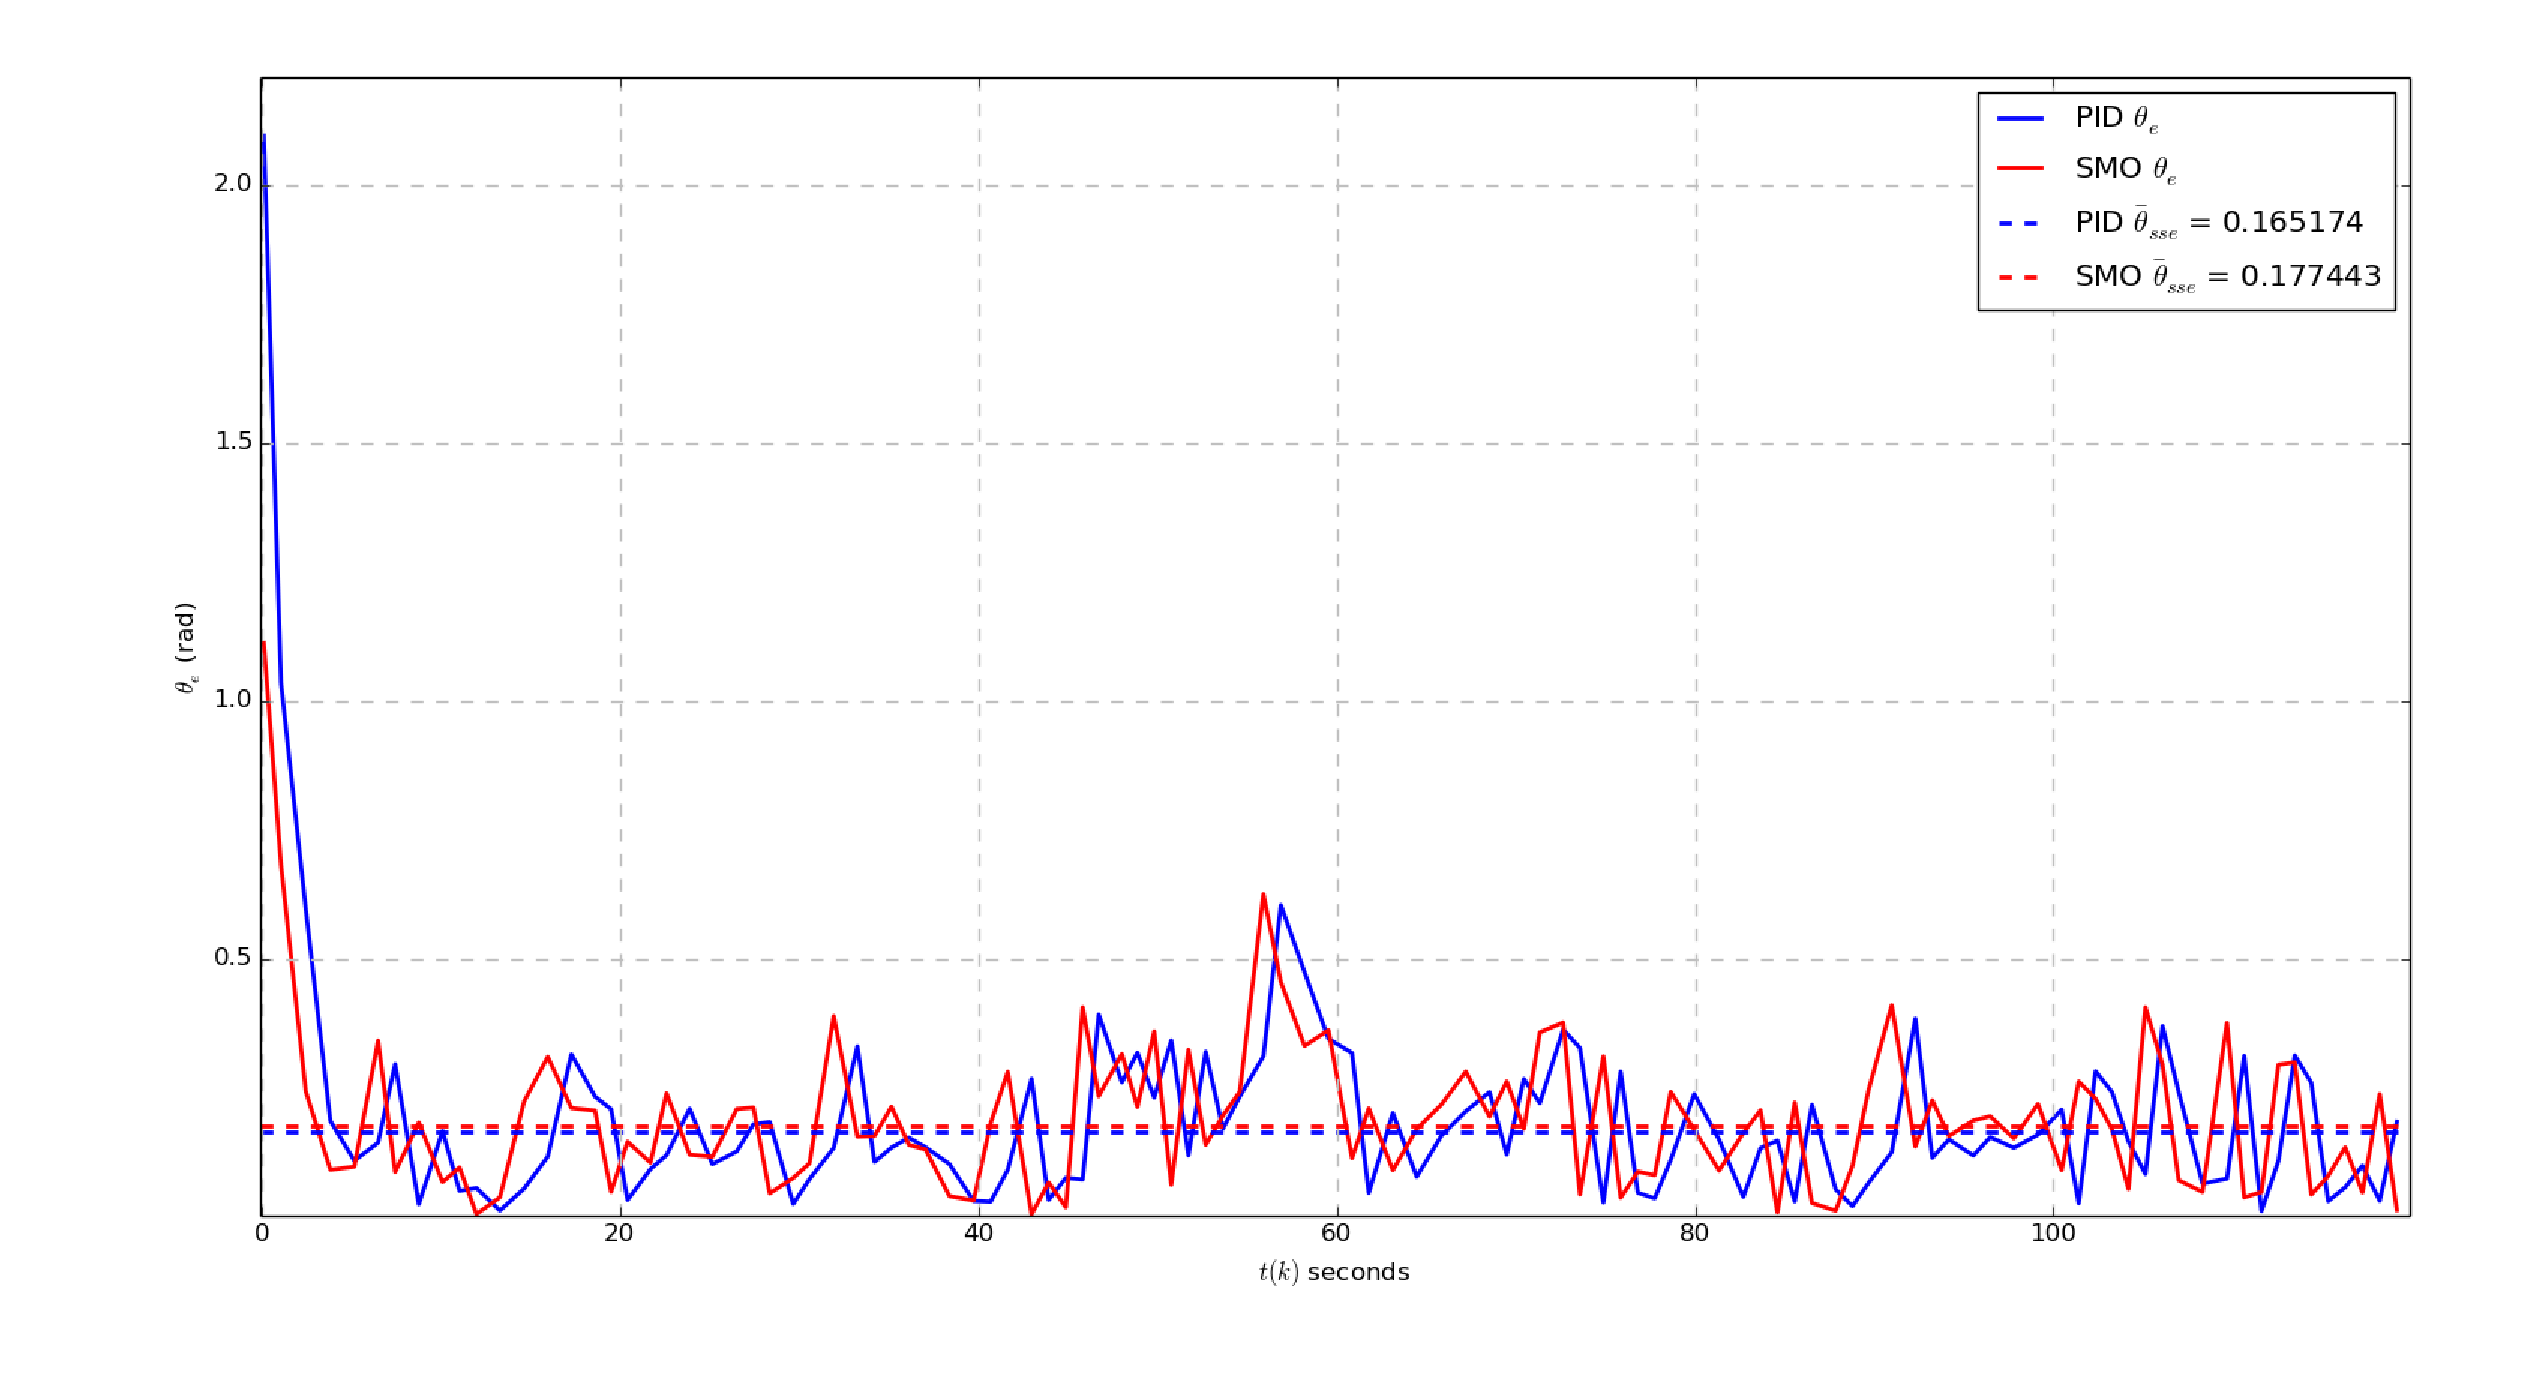
\psfig{file=figures/estimator_comparison.eps,width=6in}}
  \caption{PID/SMO Estimator Concurrent Comparison}
  \label{fig:PIDSMOEstimatorConcurrentComparison}
\end{figure}

The results in Figure \ref{fig:PIDSMOEstimatorConcurrentComparison} were generated through the TSatPy application with the script below.  Lines 10-15 define the two estimators to use in the simulation.  More can be added including the same estimator type with varied parameters.  Lines 17-19 define the system clock behavior.  The simulation will run for a simulated 120 seconds as verified in the results above.  The time steps for each update will vary between 0.8 and 1.2 seconds randomly.  And since this is running as a simulation instead of pulling data from the physical TableSat, the clock can be sped up to run at 20x speed improving the rate of the iterative testing cycle.

\begin{singlespace}
  \begin{minted}[mathescape,linenos,numbersep=10pt,frame=lines,framesep=2mm]{python}
from TSatPy import Estimator, State
from TSatPy.Clock import Metronome
import numpy as np
import matplotlib.pyplot as plt
import time
import random

print('PID / SMO Estimator Faceoff')

configs = [{'type': 'pid',
 'args': {'kpq': 0.0735,'kpw': 0.7,'kiq': 0.000863,
          'kiw': 0,'kdq': 0.00812,'kdw': 0}
},{'type': 'smo',
 'args': {'Lq': 0.282, 'Lw': 0.444, 'Kq': 0.307, 'Kw': 0.464,
    'Sq': 0.886, 'Sw': 0.569}}]

run_time = 120
speed = 20
dts = [0.8, 1.2]
c = Metronome()
c.set_speed(speed)
I = [[2, 0,  0], [0, 2, 0], [0, 0, 2]]

def setup_estimators(configs):
    x_ic = State.State()
    plant_est = State.Plant(I, x_ic, c)

    est = Estimator.Estimator(c)
    for config in configs:
        est.add(config['type'], plant_est, config['args'])

    return est

def run_comparison(est):
    x_ic = State.State(
        State.Quaternion([0,0,1], radians=4),
        State.BodyRate([0,0,0.314]))
    plant = State.Plant(I, x_ic, c)

    ts = []; smo_err = []; pid_err = []
    start_time = c.tick()
    end_time = c.tick() + run_time
    while c.tick() < end_time:
        plant.propagate()
        offset = np.random.randn() * 20 / 180.0 * np.pi
        q_noise = State.Quaternion([0,0,1], radians=offset) * plant.x.q

        x_m = State.State(q_noise, plant.x.w)

        est.update(x_m)
        ts.append(c.tick() - start_time)

        for model in est.estimators:
            q_e = State.QuaternionError(model.x_hat.q, plant.x.q)
            e, r = q_e.to_rotation()

            if type(model) is Estimator.PID:
                pid_err.append(r)
            elif type(model) is Estimator.SMO:
                smo_err.append(r)
        random.shuffle(dts)
        time.sleep(dts[0] / float(speed))

    return ts, pid_err, smo_err

def graph_it(ts, pid_err, smo_err):
    # Generate the graph here
    # See appendix for the full script

def main():
    est = setup_estimators(configs)
    graph_it(*run_comparison(est))
    return 0

if __name__ == '__main__':
    exit(main())
  \end{minted}
\nocite{minted}
\end{singlespace}

The NASA MMS TableSat 1A controller has performance requirements based off of NASA MMS's mission parameters.  Section \ref{sec:ComparativeAnalysysofPIDandSMOEstimators} demonstrated that multiple estimators can be run in parallel during both simulations and experimental runs.  As discussed above, this allows for a better insight into performance differences in estimation methods.  An additional benefit to running the controller through TSatPy is the ability to perform estimator scheduling.  Like gain scheduling which for an estimator or controller can modify what gains it uses depending on the current performance, estimator scheduling allows for switching between disparate estimation techniques during run-time.  For example, one estimator tuned for responding to large errors and run along side an estimator tuned for steady state performance.  The control algorithm can then receive more accurate state estimates on a wider range of environmental conditions.


\chapter{CONTROLLERS}
\label{chap:Controllers}

The control requirements for NASA MMS TableSat IA can be simplified into three main goals.

The first is to maintain a steady spin rate of 3 rpm ($\pi/10$ rad/sec).  Given the relative success of the body rate estimation in Chapter \ref{chap:Estimators}, this goal should be attainable without the need of advanced control efforts.

The second is to correct for any nutation wobble about the $x$ and $y$ body axes.  This requirement essentially can be seen as driving body rates $\omega_y$ and $\omega_z$ to zero and ensuring the estimated quaternion's Euler axis is kept in line with the global reference frame's $z$-axis.

The third is to prevent and/or remove oscillations in the Axial Double Probe (ADP) and Spin-plane Double Probe (SDP) booms.  Out of the three, this performance goal has the largest set of dependencies for success.  This level of control is reliant on effective actuators along with reliable state estimates based on an accurate system model which include flexible boom dynamics.

The first two goals are addressed in this chapter as their scope is limited to controller design.  Section \ref{sec:ActuatorConfiguration} covers the configuration of the actuators on TableSat and how their configuration is incorporated into the controller code.  The remaining sections of this chapter focus on rate and nutation control methods.  in this part of the research it is assumed that the estimators provide perfect state estimates.  These conditions temporarily limit the scope of the testing to ensure that the control techniques are being implemented properly in the software especially since with the development of some non-standard techniques.  The third goal, controlling boom oscillations, is addressed in Chapter \ref{chap:ObserverBasedControls} when multiple modules are linked together to obtain a wider view of the interactions between observer-based controllers being acted upon by noisy state measurements.

\section{Actuator Configuration}
\label{sec:ActuatorConfiguration}

As shown in Figure \ref{fig:TSatThrusters}, the actuators on NASA MMS TableSat IA consist of four single directional computer fans.  Two are oriented for rate control and two for nutation control.  The body rate control fans are mounted on opposite sides of the bus with their thrusts applying opposing moments.  The two nutation fans are mounted flush with the bus at a 90 degree offset and have their thrust directed downward.  The fans are assumed to be mounted such that the moments are applied about orthogonal axes.  This simplifies the actuator module's voltage input calculations for each fan which can be improved if testing shows that the effects from the off center are significant enough to compensate for.  Four analog ports to the Athena PC are available for actuator usage after mounting the sensors.  Two are dedicated to the rotational fans to provide full rotational control, and the remaining two provide limited nutation control.
\begin{figure}[H]
  \centerline{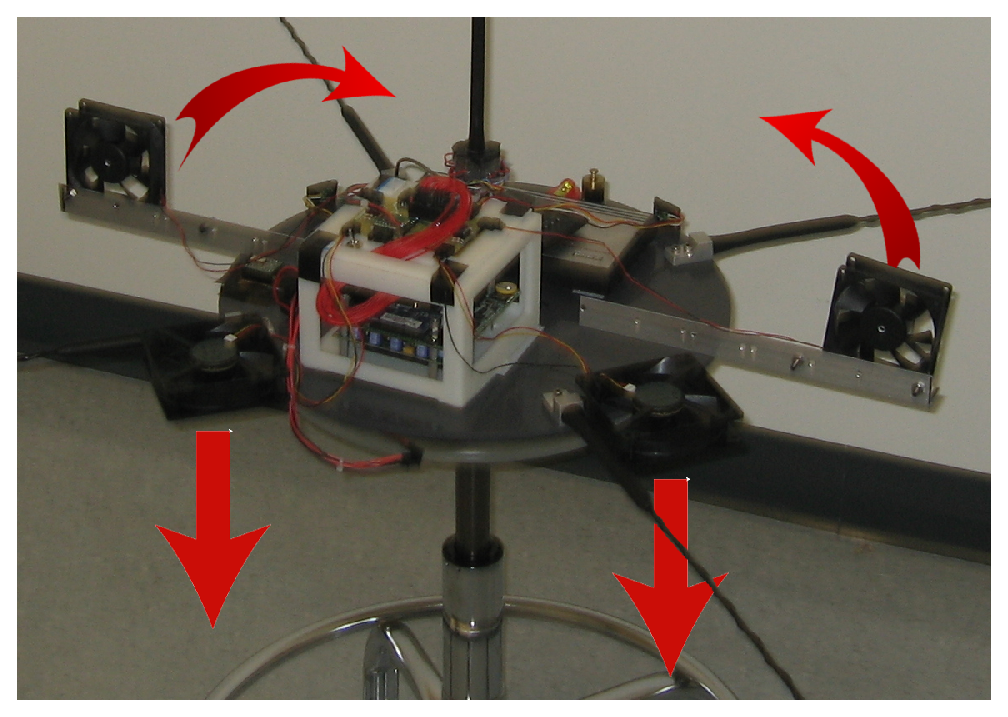
\psfig{file=figures/tsat_thrusters.eps,height=3in}}
  \caption{NASA MMS TableSat IA thrusters}
  \label{fig:TSatThrusters}
\end{figure}
Sending the desired moment control commands from the controller directly to the estimator without taking the fan geometry into consideration creates a disconnect between the estimated and actual system states.  The software's actuator module is designed to accept a list of fans with their center, direction of thrust related to the body reference frame, and maximum force to determine the moments couples that are actually possible.
\begin{figure}[H]
  \centerline{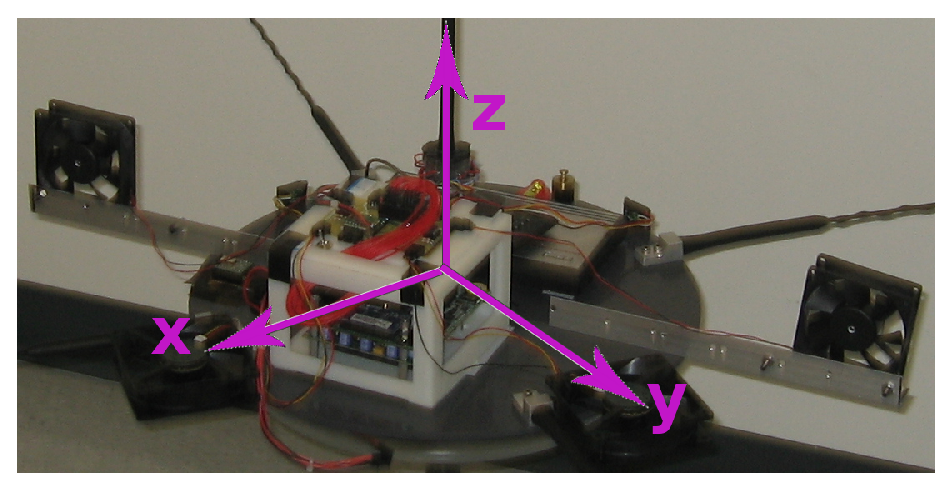
\psfig{file=figures/tsat_body_axes.eps,height=3in}}
  \caption{NASA MMS TableSat IA Body Axes}
  \label{fig:TableSatBodyAxes}
\end{figure}
Table \ref{tbl:ActuatorConfiguration} shows the fan configuration for the NASA MMS TableSat IA as arranged in Figure \ref{fig:TSatThrusters}.
\begin{table}[H]
  \centering
  \begin{tabular}{c|c|c|c|c}
    Fan & Center $\bs{f_c}$ (m) & Direction $\bs{n}$ & $F$ (N) & Max Moment $\frac{F \bs{n} \times \bs{f_c}}{|\bs{n}|}$ (Nm) \\ \hline
    1 & $(0.2474, -0.2474, 0)$ & $(-1, -1, 0)$ & 0.08 & $(0, 0, 0.039598)$ \\
    2 & $(-0.2474, 0.2474, 0)$ & $(-1, -1, 0)$ & 0.08 & $(0, 0, -0.039598)$ \\
    3 & $(0.25, 0, 0)$ & $(0, 0, -1)$ & 0.08 & $(0.02, 0, 0)$ \\
    4 & $(0, 0.25, 0)$ & $(0, 0, -1)$ & 0.08 & $(0, -0.02, 0)$ \\
  \end{tabular}
  \caption{Actuator configuration}
  \label{tbl:ActuatorConfiguration}
\end{table}
The algorithm shown in Snippet \ref{code:actuator_usage} demonstrates the actuator module's functionality implemented in the TSatPy software.  Lines 4-13 define the geometry of the actuators displayed in Figure \ref{fig:TSatThrusters} with the addition of a hypothetical fifth actuator along with their center, direction of thrust, and maximum thrust force.


\begin{listing}
\begin{singlespace}
  \begin{minted}[mathescape,linenos,numbersep=10pt,frame=lines,framesep=2mm]{python}
import numpy as np
from TSatPy.Actuator import Actuator

configs = [{'type': 'fan', 'args': {'name': 'CW',
  'center': (0.2474, -0.2474, 0), 'direction': (-1, -1, 0), 'F': 0.08}
},{'type': 'fan', 'args': {'name': 'CCW1',
  'center': (-0.2474, 0.2474, 0), 'direction': (-1, -1, 0), 'F': 0.08}
},{'type': 'fan', 'args': {'name': 'CCW2',
  'center': (-0.2474, -0.2474, 0), 'direction': (1, -1, 0), 'F': 0.08}
},{'type': 'fan', 'args': {'name': 'NY', 'center': (0.25, 0, 0),
  'direction': (0, 0, 1), 'F': 0.08}
},{'type': 'fan', 'args': {'name': 'NX', 'center': (0, 0.25, 0),
  'direction': (0, 0, 1), 'F': 0.08}}]

def set_level(act, power_level):
    print 'Setting power level=%g for: %s' % (power_level, act)

def setup_actuators(configs):
    act = Actuator()
    for config in configs:
        act.add(config['type'], set_level, config['args'])
    return act

act = setup_actuators(configs)
print(act)
M = np.mat([0.03, 0.11, 0.04]).T
print("Request moment: %s" % (M.T))
print("Applied moment: %s" % (act.request_moment(M).T))

# Prints Out
# Actuator
#  <Fan CW moment=(0, -0, -0.0279901)>
#  <Fan CCW1 moment=(0, 0, 0.0279901)>
#  <Fan CCW2 moment=(0, 0, 0.0279901)>
#  <Fan NY moment=(0, -0.02, 0)>
#  <Fan NX moment=(0.02, 0, 0)>
# Request moment: [[ 0.03  0.11  0.04]]
# Setting power level=1 for: <Fan NX moment=(0.02, 0, 0)>
# Setting power level=0.714538 for: <Fan CCW1 moment=(0, 0, 0.0279901)>
# Setting power level=0.714538 for: <Fan CCW2 moment=(0, 0, 0.0279901)>
# Applied moment: [[ 0.02  0.    0.04]]
  \end{minted}
\caption{Moment to actuator voltage conversion}
\label{code:actuator_usage}
\nocite{minted}
\end{singlespace}
\end{listing}

At line 24, the actuator instance is created and each fan's potential contribution to the overall control moment is calculated with
\begin{equation}
  \bs{M} = \frac{F \bs{n} \times \bs{f_c}}{|\bs{n}|}
\end{equation}
where the moment couple $\bs{M}$ is calculated from the max actuator force $F$, the direction of the thrust $\bs{n}$, and $\bs{f_c}$ is fan's center relative to the center of rotation.
The script output shown in Snippet \ref{code:actuator_usage} describes how a requested moment of $M_x = 0.03Nm, M_y = 0.11Nm, \text{ and } M_z = 0.04Nm$ is applied to the five-fan configuration.  The ``Nx'' fan can only produce a $0.02Nm$ moment, so it is set to full power to supply part of the requested $M_x = 0.03Nm$.  The ``Ny'' fan does not contribute since it's thrust is in the opposite direction from the needed $M_y = 0.11Nm$.  The ``CCW1'' and ``CCW2'' fans can not individually meet the requested $M_z = 0.04Nm$, but they are able to collaboratively reach the requested moment by contributing 71\% each.  In the end, the actual moment that is applied to the TableSat is $M_x = 0.02Nm, M_y = 0Nm, M_z = 0.04Nm$.  This actual moment is converted to equivalent voltage commands to be transmitted to the TableSat, and supplied to the estimator to propagate its dynamics.

\section{Rate Control}
\label{sec:RateControl}

The first of the three controls goals introduced at the start of this chapter is to control the TableSat to maintain a desired body rate of $\bs{\omega}_d$ such that
\begin{equation}
  \bs{\omega}_d = 0 \bs{i} + 0 \bs{j} + 0.314 \bs{k}
\end{equation}
This desired rate is used for the tests in Sections \ref{subsec:PRateControl} through \ref{subsec:SlidingModeController}.  As explained previously, all body rate controllers are tested under the assumption of perfect observer state feedback to ensure appropriate functionality before combining with other modules for observer-based control.
\subsection{P Rate Controller}
\label{subsec:PRateControl}
The initial controller tested is the proportional body rate controller of the form
\begin{equation}
  \bs{M}_{\omega} = \bs{K}_{\omega p} \left( \bs{\hat{\omega}} - \bs{\omega}_d \right)
  \label{eqn:PRateControl}
\end{equation}
Through a series of simulations with randomized initial conditions for body rates a gradient descent based on minimizing control effort is used to tune the proportional gains to
\begin{equation}
  \bs{K}_{\omega p} = \begin{bmatrix} 0.404 & 0 & 0 \\ 0 & 0.463 & 0 \\ 0 & 0 & 0.428 \end{bmatrix}
\end{equation}
Figure \ref{fig:PRateControl} shows the body rates and applied moments for one of the the optimized gain tests.  The results show an adequate level of control that damps out nutations and maintains the $\omega_z = 0.314$ rad/sec design requirement.
\begin{figure}[H]
  \centerline{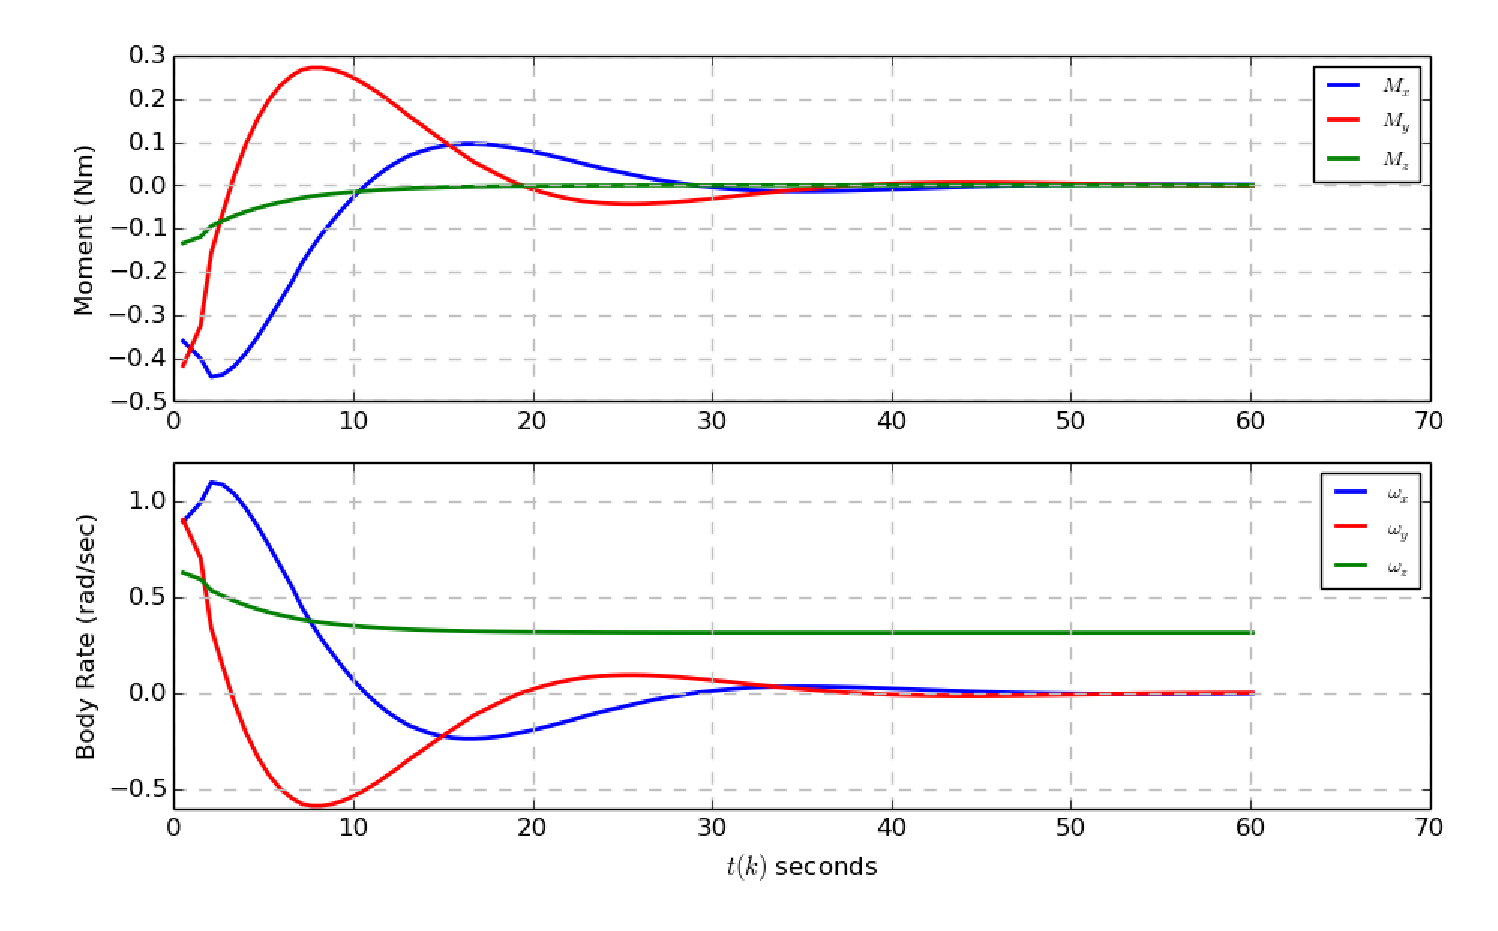
\psfig{file=figures/p_rate_control.eps,width=6in}}
  \caption{P rate control}
  \label{fig:PRateControl}
\end{figure}

\subsection{PID Rate Controller}
\label{subsec:PIDRateControl}

Expanding the proportional controller to include the integral and derivative term as shown in Equation (\ref{eqn:PIDRateControl}) can improve the performance slightly in tests with perfect measurement tests, but more importantly provides tools for dealing with noisy measurements when assessing observer-based controllers in Chapter \ref{chap:ObserverBasedControls}.  The integral and derivative terms are implemented with the $\Delta t_k$ adaptive step, as with the PID estimator, to help take into account inconsistencies in update intervals by tracking the step size at each update the resulting control algorithm is
\begin{equation}
  \begin{aligned}
    \bs{M}_{\omega} &= \bs{K}_{\omega p} \bs{\omega}_e + \bs{K}_{\omega i} \cdot (\Delta t_k \bs{I})\cdot \bs{\omega}_e + \bs{K}_{\omega d} \cdot \left(\frac{1}{\Delta t_k} \bs{I}\right) \cdot \bs{\omega}_e
  \end{aligned}
  \label{eqn:PIDRateControl}
\end{equation}
\begin{figure}[H]
  \centerline{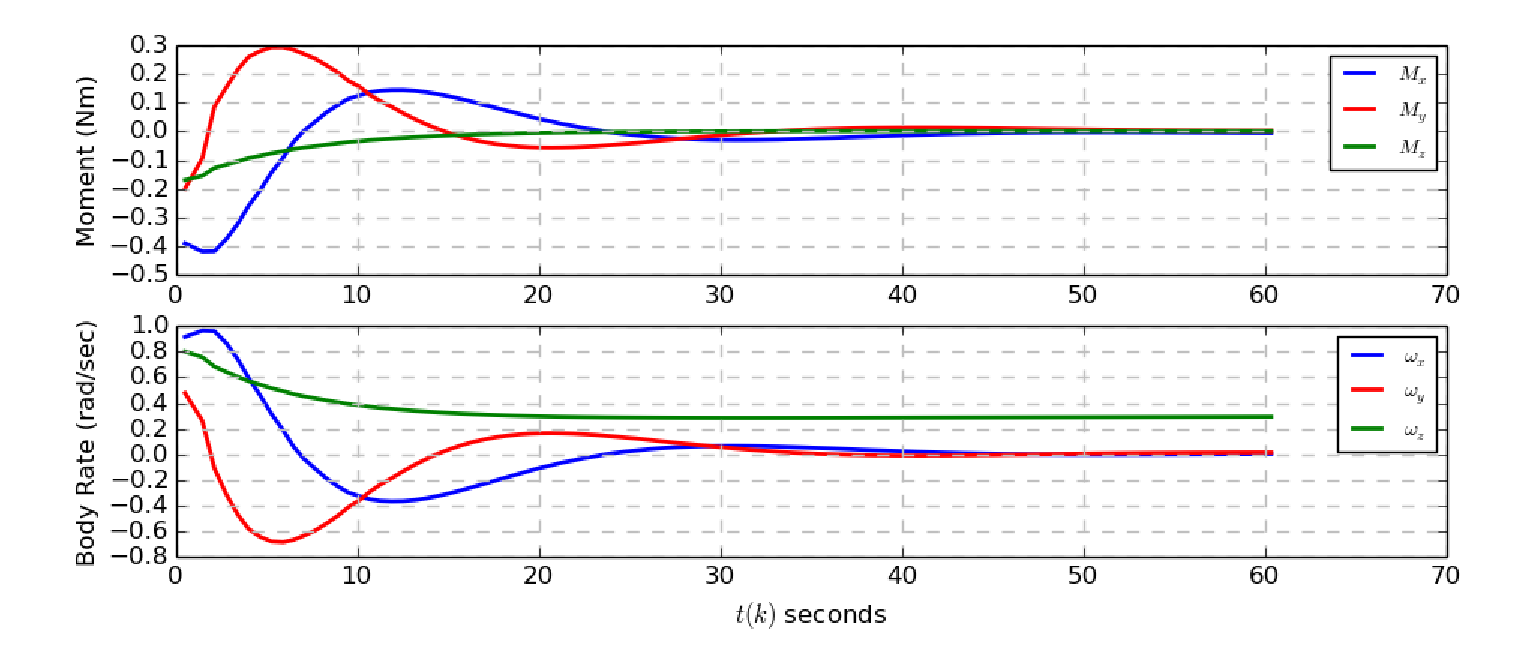
\psfig{file=figures/pid_rate_control.eps,width=6in}}
  \caption{PID rate control}
  \label{fig:PIDRateControl}
\end{figure}
The response curve in Figure \ref{fig:PIDRateControl} is generated from a random set of initial condition, and with the PID gains of Equation (\ref{eqn:PIDRateControlGains}) tuned through gradient descent iterations based on minimizing the total control effort.  In the case of perfect measurements, the two addition correctional control terms generally reduce the overshoot of the response but do not significantly decrease the settling time.
\begin{equation}
  \begin{aligned}
    \bs{K}_{\omega p} &= \begin{bmatrix} 0.424 & 0 & 0 \\ 0 & 0.416 & 0 \\ 0 & 0 & 0.346 \end{bmatrix},
    \bs{K}_{\omega i} = \begin{bmatrix} 0.006 & 0 & 0 \\ 0 & 0.003 & 0 \\ 0 & 0 & 0.005 \end{bmatrix} \\
    \bs{K}_{\omega d} &= \begin{bmatrix} 0.044 & 0 & 0 \\ 0 & 0.072 & 0 \\ 0 & 0 & 0.042 \end{bmatrix}
  \end{aligned}
  \label{eqn:PIDRateControlGains}
\end{equation}
Figure \ref{fig:PIDRateControlMoments} shows how the moments from each of the PID components contribute to the overall moments applied.  The addition of the derivative term gives the system a slightly quicker response than that with just the P-controller.   In this perfect measurement scenario the the overall performance of the system would benefit from the integral term being removed altogether since it does not contribute much to the initial response and even causes a larger steady state error than the P-controller.
\begin{figure}[H]
  \centerline{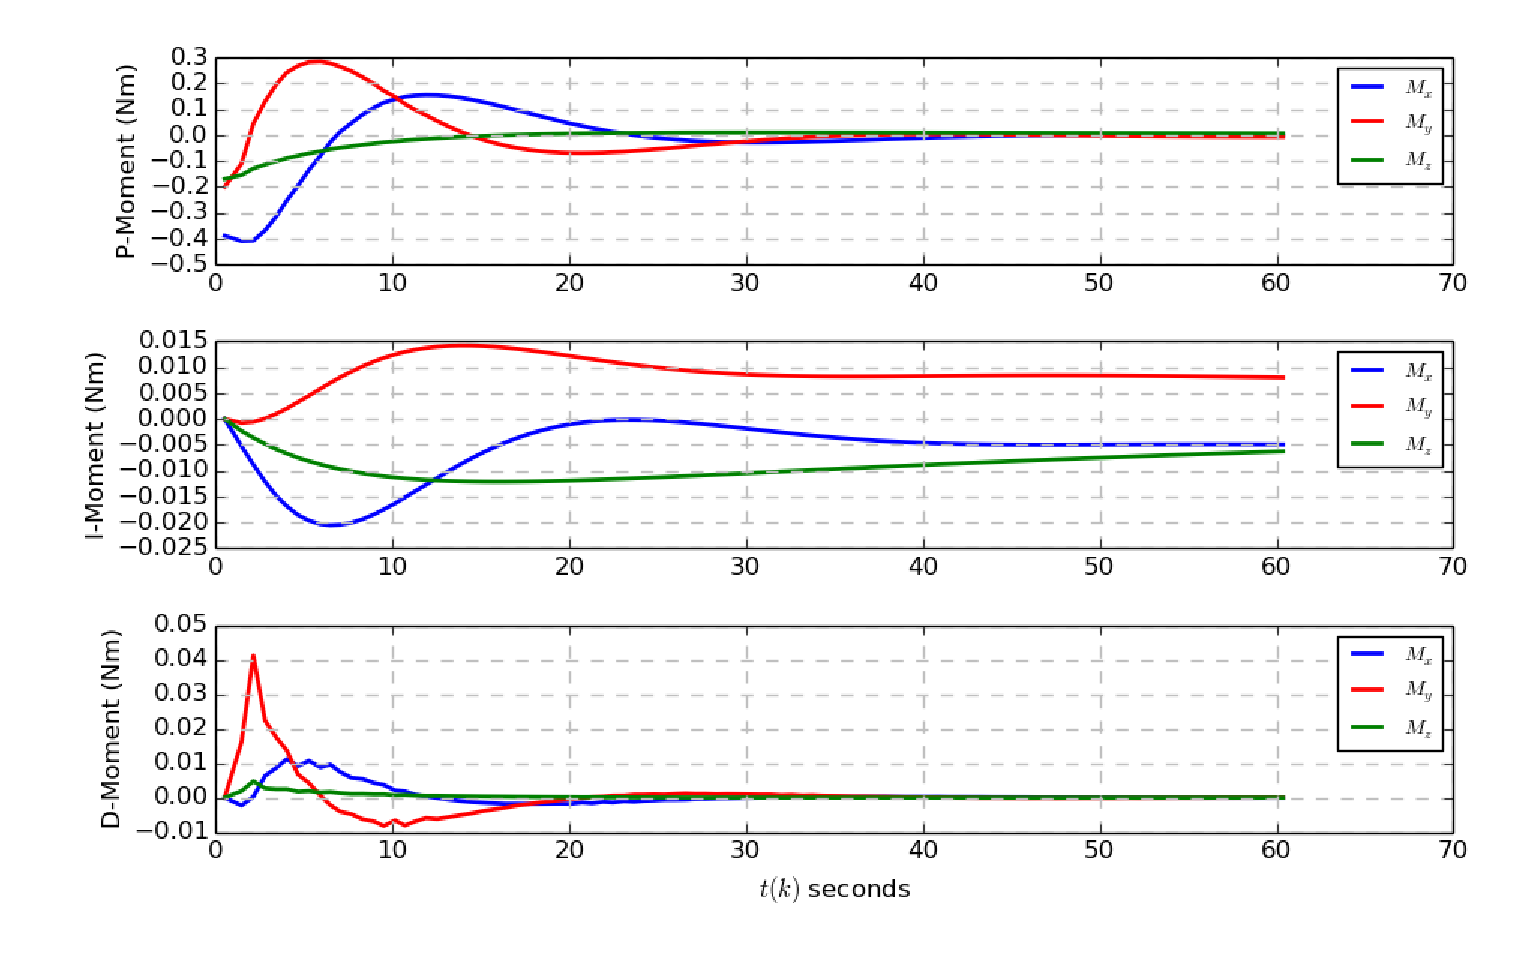
\psfig{file=figures/pid_rate_control_moments.eps,width=6in}}
  \caption{PID rate control moments}
  \label{fig:PIDRateControlMoments}
\end{figure}

\subsection{Sliding Mode Controller}
\label{subsec:SlidingModeController}

The Sliding Mode Controller (SMC) operates similarly to a proportional controller and is governed by the equation
\begin{equation}
  \bs{M}_{\omega} = \bs{L}_{\omega} \bs{\omega}_e + \bs{K}_{\omega}\bs{1}_s \big(\bs{\omega}_e \big)
  \label{eqn:SMController}would
\end{equation}
where $\bs{L}_{\omega}$ is the proportional switching gain and the $\bs{1}_s$ function is a switching finction that can take a number of forms, such as the signum and arctangent functions.  In this thesis, the SMC uses the saturation function such that $\bs{1}_s$ is
\begin{equation}
  \bs{1}_s \big(\bs{\omega}_e \big) = sat \begin{bmatrix} \omega_{ex} / S_{\omega} &0 &0 \\ 0 & \omega_{ey} / S_{\omega} & 0 \\ 0 & 0 & \omega_{ez} / S_{\omega} \end{bmatrix}
\end{equation}
The SMC response in Figures \ref{fig:SMCRateControl} and \ref{fig:SMCRateControlMoments}, is generated with the following gain values tuned through a gradient descent search that minimizes control effort.
\begin{equation}
    \bs{L}_{\omega} = \begin{bmatrix} 0.3983 & 0 & 0 \\ 0 & 0.3828 & 0 \\ 0 & 0 & 0.4160 \end{bmatrix},
    \bs{K}_{\omega} = \begin{bmatrix} 0.4399 & 0 & 0 \\ 0 & 0.5097 & 0 \\ 0 & 0 & 0.3162 \end{bmatrix},
    S_{\omega} = 0.1404
  \label{SMCRateControlGains}
\end{equation}
The response to the test configuration shows significant improvements in performance over the P and PID rate controller as shown if Figure \ref{fig:SMCRateControl}.
\begin{figure}[H]
  \centerline{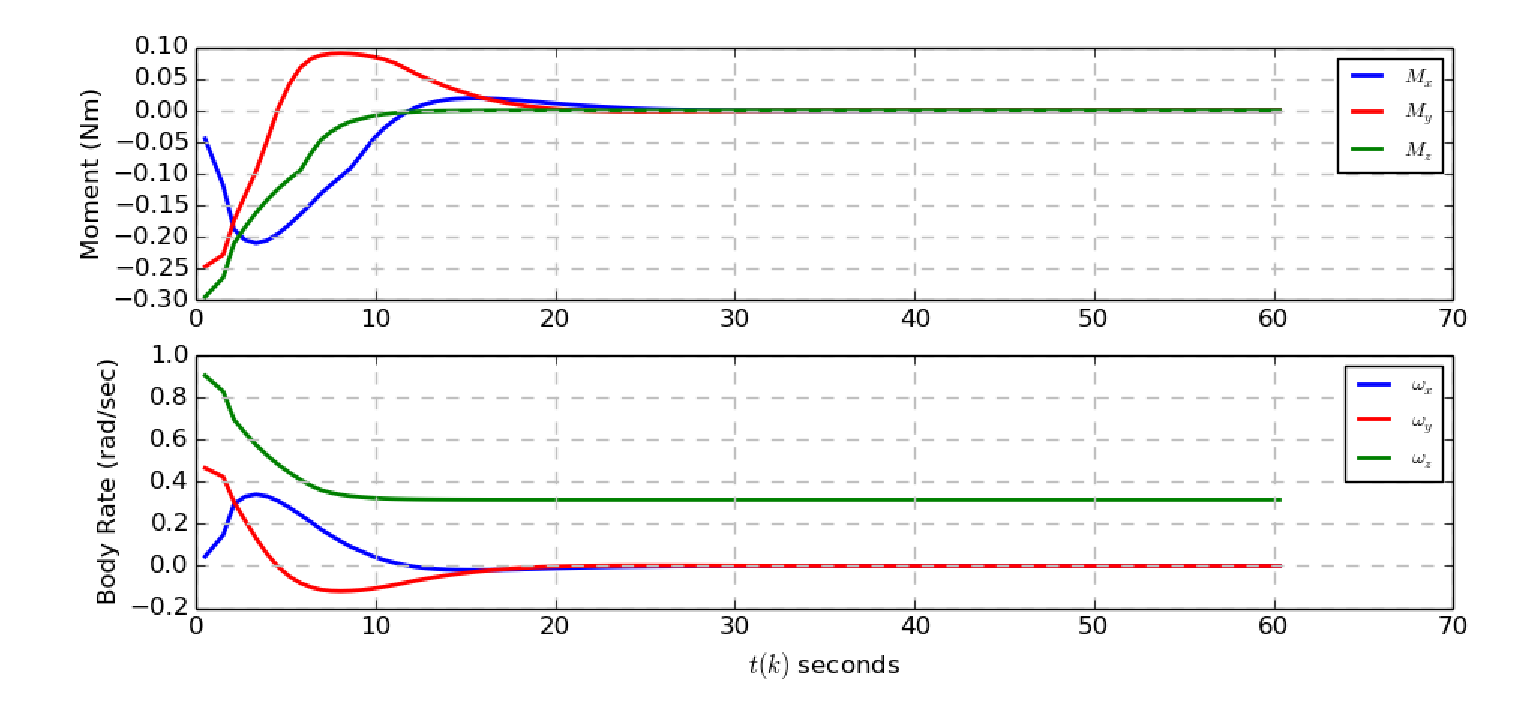
\psfig{file=figures/smc_rate_control.eps,width=6in}}
  \caption{SMC rate control}
  \label{fig:SMCRateControl}
\end{figure}
The moment graph in Figure \ref{fig:SMCRateControl} is a combination of the two terms in the SMC.  Breaking those overall moment values into the separate term's contributions (Figure \ref{fig:SMCRateControlMoments}) shows the similar profile between the proportional and saturation term contributions with the exception of the peaks missing from the saturation response.
\begin{figure}[H]
  \centerline{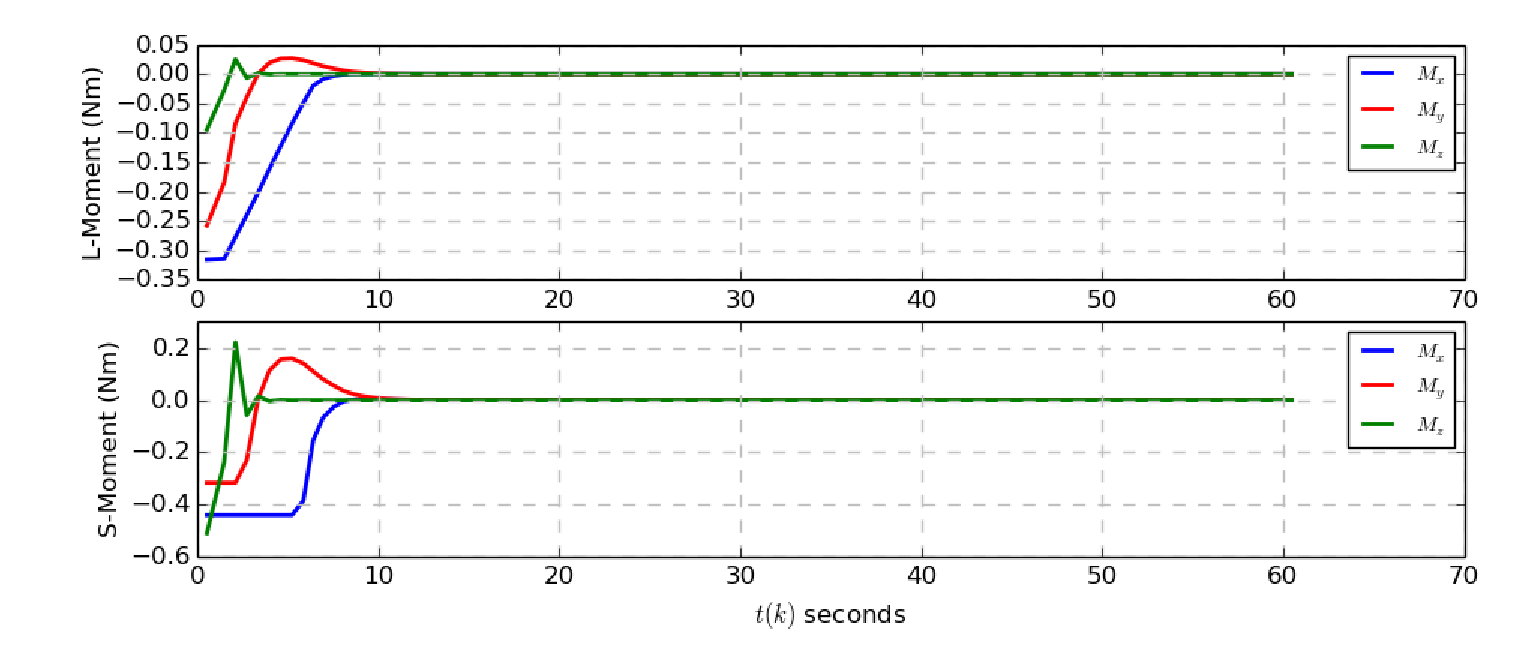
\psfig{file=figures/smc_rate_control_moments.eps,width=6in}}
  \caption{SMC rate control moments}
  \label{fig:SMCRateControlMoments}
\end{figure}
With assumed perfect state feedback, the saturation term adds a significant performance improvement over the P and PID implementations.  Additionally, with two fewer design gains, tuning the SMC is slightly less involved than the PID body rate controller.

\section{Quaternion to Moment Conversion}
\label{sec:QuaternionToMomentConversion}

The remainder of this chapter focuses on the attitude control problem to correct for nutation (Section \ref{sec:AttitudeAndNutationControl}) and the integration of the attitude and rate controller (Section \ref{sec:AttitudeandBodyRateControl}).  The proper conversion from an attitude error measurement to actuator moments is critical to providing a robust control method.

The attitude error measurement is calculated through the quaternion multiplicative method as is established in Section \ref{sec:HighIntegrityStateAdjustments}:

\begin{equation}
  \bs{q}_e = \bs{q}_d^* \otimes \bs{\hat{q}}
\end{equation}

Unlike with the estimator where the input and output formats are both quaternions, the quaternion error in the controller $\bs{q}_e$ is composed of four parameters that need to map to three moments values.  The commonly used method for this is to fall back on matrix algebra where $\bs{K}_q \in \Re^{3x4}$

\begin{equation}
  \bs{M}_q = \begin{bmatrix} 3 \times 4 \end{bmatrix} \begin{bmatrix} q_1 & q_2 & q_3 & q_0 \end{bmatrix}^T
  \label{eqn:traditional_attitude_controller}
\end{equation}

There are two main issues with this approach.  First, the quaternion parameters are sinusoidal in nature.  As such, during the conversion to moment values through matrix multiplication, the magnitude of the moment does not scale linearly with that of the attitude error.

The second issue is that the quaternion is comprised of a vector and scalar that provide two separate types of information about the attitude error.  Lumping the two together in a single matrix multiplication operation ignores the physical representation of their values.  The vector defines the Euler axis which gives the attitude error its direction.  A vector component with $q_1 = q_3 = 0, q_2 \ne 0$ means that to move the estimated satellite attitude to the desired attitude requires a rotation about just the body-fixed $y$-axis which requires a moment couple in just $M_y$.  This can be represented simply as
\begin{equation}
  \bs{M}_{q} = k\bs{v}_e
\end{equation}
This provides a basis for the direction of the moment couple.  However, since the rotational quaternion is fixed at a unit norm, the magnitude of the vector component $\bs{v}_e$ varies with the size of the error.  This is compensated for by normalizing the vector such that the moment is now chosen to equal
\begin{equation}
  \bs{M}_{q} = k\bs{\hat{e}}_e
  \label{eqn:quat_vector_to_moment}
\end{equation}
where $\bs{\hat{e}}_{e}$, the Euler axis, is the normalized vector component of the quaternion.

With Equation (\ref{eqn:quat_vector_to_moment}) establishing the direction of the axis of the actuator moments, one now needs only to determine how to scale the moment couples in relation to the size of the error.  The remaining $q_0$ quantity is a reasonable first choice and the moment is now chosen to equal
\begin{equation}
  \bs{M}_{q} = kq_{0e} \bs{\hat{e}}_e
\end{equation}
where $q_{0en}$ is the scalar component of the error quaternion.

$q_{0e}$, as with the vector, is a sinusoidal measure.  The underlying rotation angle $\theta$ measure of the quaternion rotation, however, is a direct measure of the attitude error.  Extracting $\theta$ measure from $q_{0e}$ and incorporating into the moment calculation yields a final choice of $\bs{M}_q$ such that
\begin{equation}
  \begin{aligned}
    \bs{M}_{q} &= k \theta \bs{\hat{e}}_e \\
    \bs{M}_{q} &= \left[- 2k \cos^{-1} (q_{0e}) \right] \bs{\hat{e}}_e
  \end{aligned}
  \label{eqn:QuaternionToMomentConversion}
\end{equation}
where $q_{0e} = \cos(-\theta_e/2)$ from the definition of a rotational quaternion.

This conversion is used throughout all attitude control calculations in the remainder of this thesis.








\section{Attitude and Nutation Control}
\label{sec:AttitudeAndNutationControl}

Section \ref{sec:RateControl} covered the design of the rate controller which addresses the first controller goal to maintain a spin rate of $\omega_z = 3$ rpm.  This section ignores the rate control requirement and focuses strictly on the attitude control problem by incorporating the quaternion to moment conversion of Equation (\ref{eqn:QuaternionToMomentConversion}) into a PID and SMC attitude controller.   Later, Section \ref{sec:AttitudeandBodyRateControl} combines the attitude and body rate controls into a single controller.

\subsection{P Attitude Control}
\label{subsec:PAttitudeControl}

Starting with a simplest design of the proportional attitude control, Equation (\ref{eqn:QuaternionToMomentConversion}) can be directly applied as
\begin{equation}
  \bs{M}_{q} = \left[- 2K_{qp} \cos^{-1} \big(q_{0e} \big) \right] \bs{\hat{e}}_e \\
  \label{eqn:PAttitudeControl}
\end{equation}
This format of the proportional controller provides a significant time savings over the traditional method described in Equation (\ref{eqn:traditional_attitude_controller}), the number of design gains is reduced from 12 gain values to tune to a single gain.

To assess the accuracy of implementation, an example is analyzed through the use of TSatPy.  A system is initialized to a state of
\begin{equation}
  \bs{x}_0 = \begin{bmatrix} 0 \bs{i} -0.0477 \bs{j} -0.477 \bs{k} +0.8778 \\ 0 \bs{i} -0.01 \bs{j} +0.2 \bs{k} \end{bmatrix}
\end{equation}
which is essentially a 1 radian rotation about the $z$-axis with a small nutation such that initial $\omega_y = -0.01$ rad/sec.  The controller,s desired state is to return to the standard attitude where the body-fixed reference frame is aligned with that of the global reference frame
\begin{equation}
  \bs{q}_d = 0 \bs{i} +0 \bs{j} +0 \bs{k} + 1
\end{equation}
The chosen proportional gain is given as
\begin{equation}
  K_{qp} = 0.04
\end{equation}
The results from the test are shown in Figure \ref{fig:PAttitudeControl}.  The total simulation time is 120 seconds.  The top graph displays the calculated moments required to compensate for the attitude error.  As expected, $M_z$ responds in the sinusoidal pattern as the P-controller overshoots the desired attitude.  The center graph displays $\theta$ and quantifies the distance between the current and desired attitude.  With this measure, it is seen that while the majority of the attitude error is linked to the rotation about the $z$-axis.  The error progressively increases through each rotation as some of the rotational motion is transferred to the out-of-plane motion (i.e. nutation).
\begin{figure}[H]
  \centerline{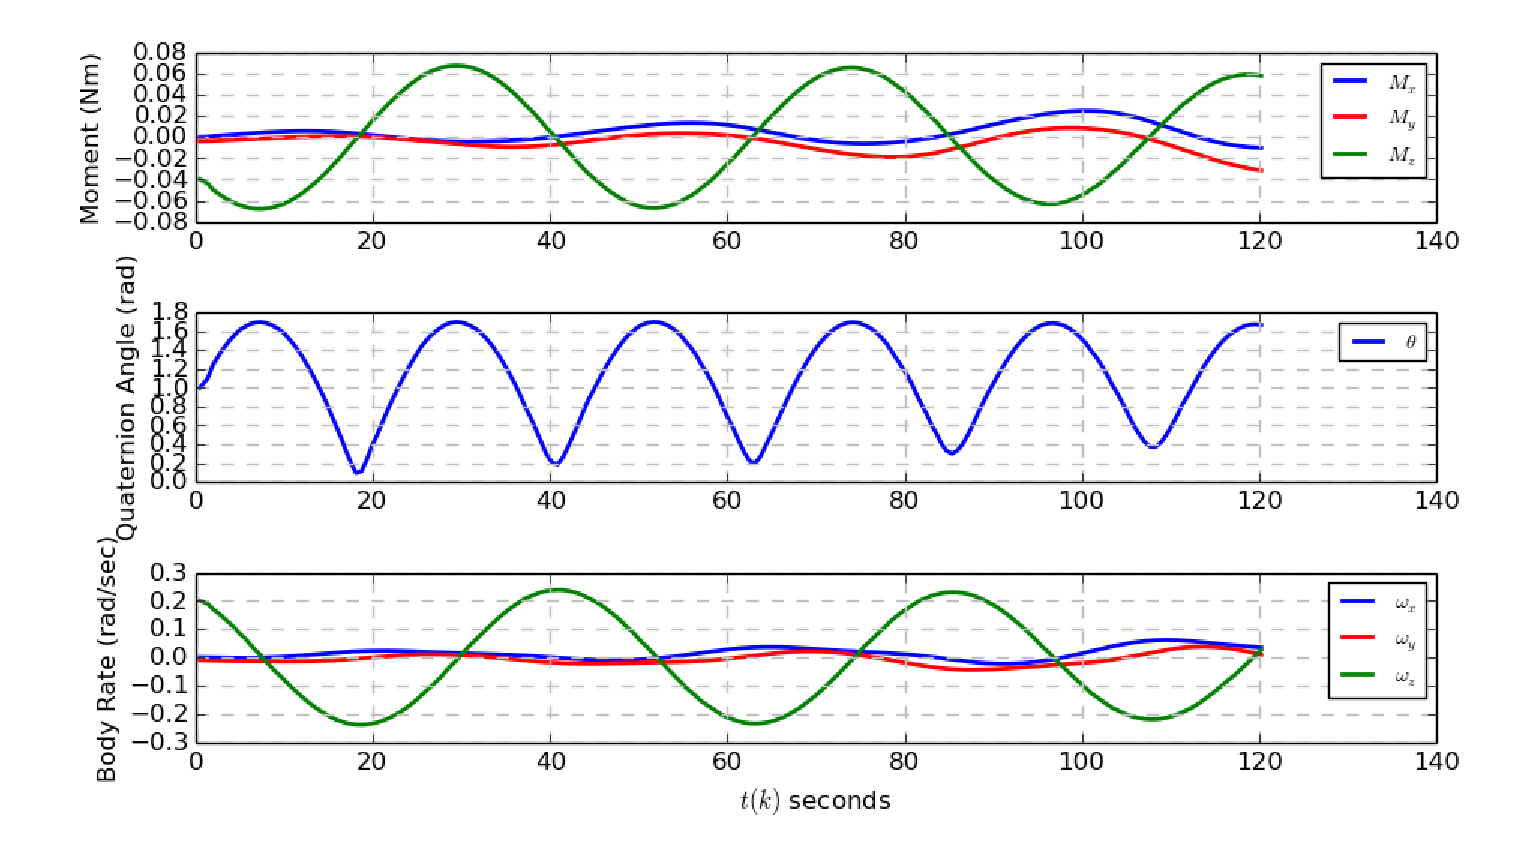
\psfig{file=figures/p_attitude_control.eps,width=6in}}
  \caption{P Attitude Control}
  \label{fig:PAttitudeControl}
\end{figure}



\subsection{Quaternion Decomposition for Nutation Control}
\label{subsec:QuaternionDecompositionForNutationControl}

Prior to combining attitude control from Section \ref{subsec:PAttitudeControl} with body rate control from Section \ref{sec:RateControl}, the controller needs to incorporate the quaternion decomposition method of Equation (\ref{eqn:quaternion_decomposition_derivation}).  The advantage to incorporating this into a controller is being able to take the quaternion portion of the state error, decompose it into its associated rotation and nutation quaternions, and replace quaternion error with the corresponding nutational quaternion error.  This attitude controller, thus, need only correct for nutation, regardless of the attitude or angular velocity.

The proportional attitude control from Equation (\ref{eqn:PAttitudeControl}) becomes
\begin{equation}
  \bs{M}_{q} = \left[-2 K_{qp} \cos^{-1} \big(q_{0en} \big) \right] \bs{\hat{e}}_{en} \\
\end{equation}
where $q_{0en}$ is the scalar component of the error quaternion's nutation component, and $\bs{\hat{e}}_{en}$ is the normalized Euler axis for the nutation component.

Snippet \ref{code:nut_from_quat} shows how with TSatPy the nutation component of the quaternion can be extracted from the state quaternion for use in moment calculations.

\begin{listing}[H]
\begin{singlespace}
  \begin{minted}[mathescape,linenos,numbersep=10pt,frame=lines,framesep=2mm]{python}
from TSatPy.State import State, Quaternion, BodyRate

print("State Error")
x_e = State(
    Quaternion([0,0.1,1],radians=1),
    BodyRate([0,-0.01,0.2]))
print("x_e: %s" % (x_e))

print("Decomposed Quaternion")
q_r, q_n = x_e.q.decompose()
print("q_r: %s" % q_r)
print("q_n: %s" % q_n)

print("Nutation Only State Error")
x_e.q = q_n
print("x_e: %s" % (x_e))

# Prints Out
# State Error
# x_e: <Quaternion [-0 -0.0477046 -0.477046], 0.877583>,
#      <BodyRate [0 -0.01 0.2]>
# Decomposed Quaternion
# q_r: <Quaternion [0 0 -0.47759], 0.878583>
# q_n: <Quaternion [-0.0227833 -0.0419125 -0], -0.998861>
# Nutation Only State Error
# x_e: <Quaternion [-0.0227833 -0.0419125 -0], -0.998861>,
#      <BodyRate [0 -0.01 0.2]>
  \end{minted}
\caption{Extracting the nutation quaternion from the state quaternion}
\label{code:nut_from_quat}
\nocite{minted}
\end{singlespace}
\end{listing}

\subsection{P Nutation Control}
\label{subsec:PNutationControl}

Using the proportional control
\begin{equation}
  \bs{M}_{q} = \left[- K_{qp} \cos^{-1} (q_{0n}) \right] \bs{\hat{e}}_n
  \label{eqn:PNutationControl}
\end{equation}
with the same initial state and desired quaternion as the proportional attitude controller from the previous example.  That is,
\begin{equation}
  \bs{x}_0 = \begin{bmatrix} 0 \bs{i} -0.0477 \bs{j} -0.477 \bs{k} +0.8778 \\ 0 \bs{i} -0.01 \bs{j} +0.2 \bs{k} \end{bmatrix}
\end{equation}
\begin{equation}
  \bs{q}_d = 0 \bs{i} +0 \bs{j} +0 \bs{k} + 1
\end{equation}
\begin{figure}[H]
  \centerline{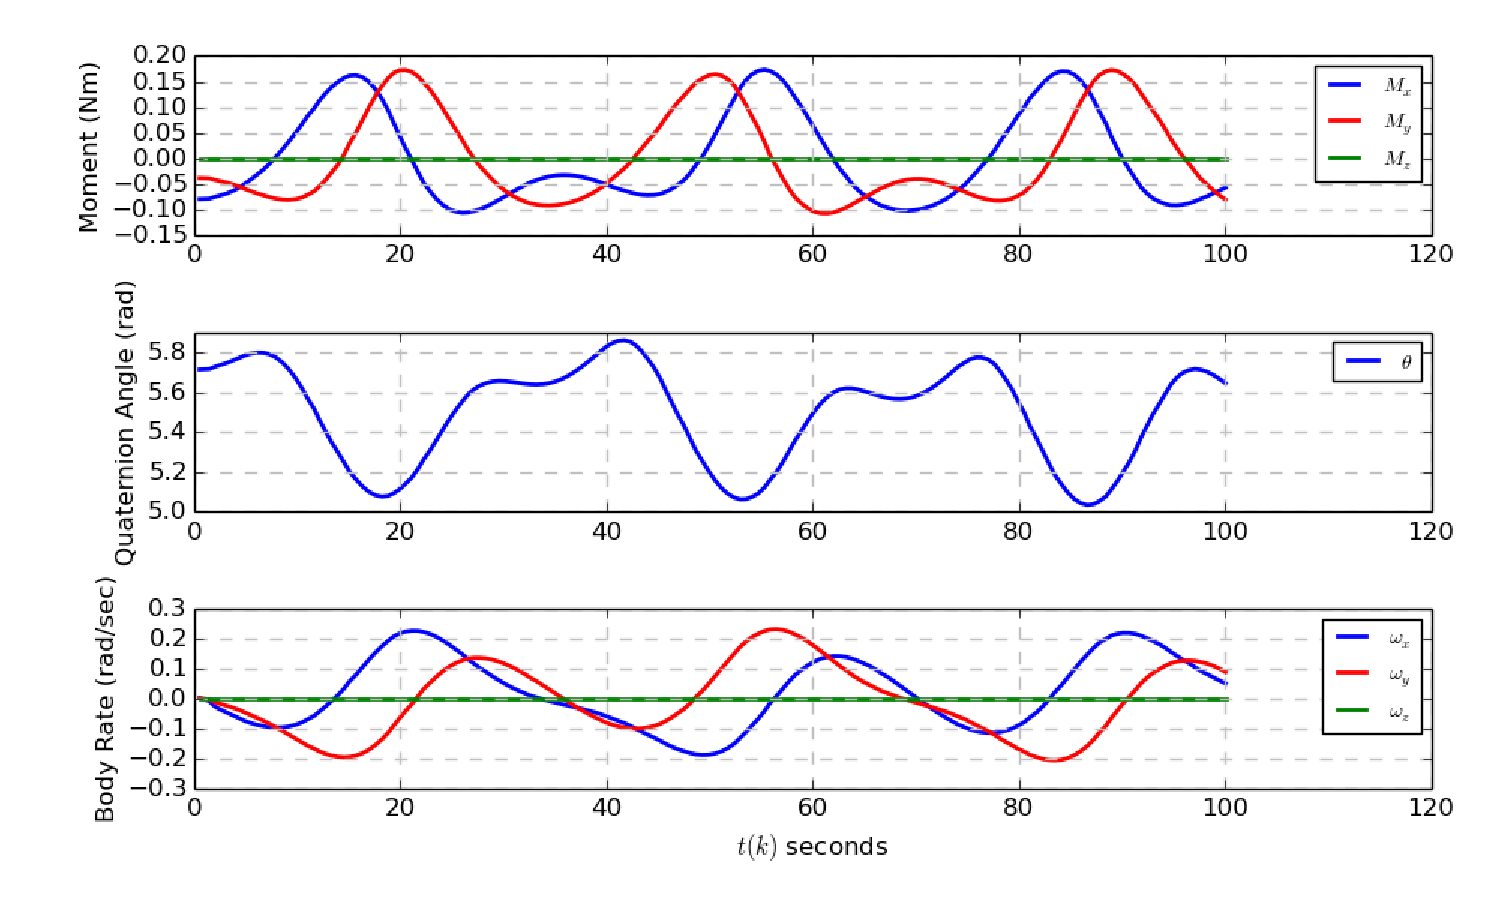
\psfig{file=figures/p_nutation_control.eps,width=6in}}
  \caption{P Nutation Control}
  \label{fig:PNutationControl}
\end{figure}
Figure \ref{fig:PNutationControl} shows the resulting control moments, quaternion angle error, and body rates with these conditions.  In the first and last plots, the body rates and moments show expected behavior, where the corrections for initial nutation cause fluctuations in $\omega_x$ and $\omega_z$ with $\omega_z$ remaining unchanged.  This means that for spin-stabilized systems like NASA's MMS Mission satellite, the controller can correct for nutation errors and is unaffected by the constant spin rate.  The same can be seen in the first graph where moments are applied about the $x$ and $y$ axes, but none are applied to control the initial spin about the $z$-axis.
The center plot tracking quaternion angle shows that while some of the nutation is removed, the proportional nutation controller is clearly not sufficient to remove all nutation.


\section{Attitude and Body Rate Control}
\label{sec:AttitudeandBodyRateControl}

Sections \ref{sec:RateControl} and \ref{sec:AttitudeAndNutationControl} have established methods to address spin rate and nutation control goals.  In this section the two are used together.  In Section \ref{subsec:FixedAttitudeControl}, the attitude and body rate controllers are combined to take a satellite from an initialized uncontrolled spin and detumble it to the standard orientation so that the body-fixed axes are aligned with the global axes.  Section \ref{subsec:SpinStabilizedControl} releases the restriction on motion about the $z$-axis and takes the satellite's initial uncontrolled spin to a nutation-free rotation about the $z$-axis.
\begin{equation}
    \bs{M} = \bs{M}_{q} + \bs{M}_{\omega}
\end{equation}
For consistency, all tests in this section are initialized with the following state
\begin{equation}
  \bs{x}_0 = \begin{bmatrix} -0.532 \bs{i} -0.417 \bs{j} -0.275 \bs{k} +0.684 \\ 0.315 \bs{i} +0.207 \bs{j} +0.113 \bs{k} \end{bmatrix}
  \label{eqn:attitude_and_body_rate_control_ic}
\end{equation}

\subsection{Fixed Attitude Control}
\label{subsec:FixedAttitudeControl}
The PID controllers are defined as
\begin{equation}
  \begin{aligned}
    \bs{M} &= \bs{M}_{q} + \bs{M}_{\omega} \\
    \bs{M}_{q} &= \left[- K_{qp} \cos^{-1} (q_{0e}) \right] \bs{\hat{e}}_e + \left[- K_{qi} \cos^{-1} (q_{0ei}) \right] \bs{\hat{e}}_{ei} + \left[- K_{qd} \cos^{-1} (q_{0ed}) \right] \bs{\hat{e}}_{ed} \\
    \bs{M}_{\omega} &= \bs{K}_{\omega p} \bs{\omega}_e + \bs{K}_{\omega i} \cdot (\Delta t_k \bs{I})\cdot \bs{\omega}_e + \bs{K}_{\omega d} \cdot \left(\frac{1}{\Delta t_k} \bs{I}\right) \cdot \bs{\omega}_e
  \end{aligned}
\end{equation}
where $\bs{\hat{e}}_e, \bs{\hat{e}}_{ei}, \text{ and } \bs{\hat{e}}_{ed}$ are the Euler axes for the quaternion error, quaternion error integral, and quaternion error derivative, respectively, with the integral $\bs{q}_{ei}$ and derivative $\bs{q}_{ed}$ quaternions from Equations (\ref{eqn:IEstimator}) and (\ref{eqn:DEstimator}).

The results from the PID body rate and attitude controller are shown in Figures \ref{fig:PIDAttitudeAndRateControl} and \ref{fig:PIDAttitudeAndRateControlMoments} and are tested with the following control gains:
\begin{equation}
  \begin{aligned}
    K_{qp} &= 0.6022,K_{qi} = 0.04656,K_{qd} = 0.8554 \\
    K_{\omega p} &= \bs{I} \begin{bmatrix} 0.70326 & 0.7203 & 0.61757 \end{bmatrix}^T \\
    K_{\omega i} &= \bs{I} \begin{bmatrix} 0.04207 & 0.06999 & 0.018591 \end{bmatrix}^T \\
    K_{\omega d} &= \bs{I} \begin{bmatrix} 0.4096 & 0.6032 & 0.6123 \end{bmatrix}^T
  \end{aligned}
\end{equation}
\begin{figure}[H]
  \centerline{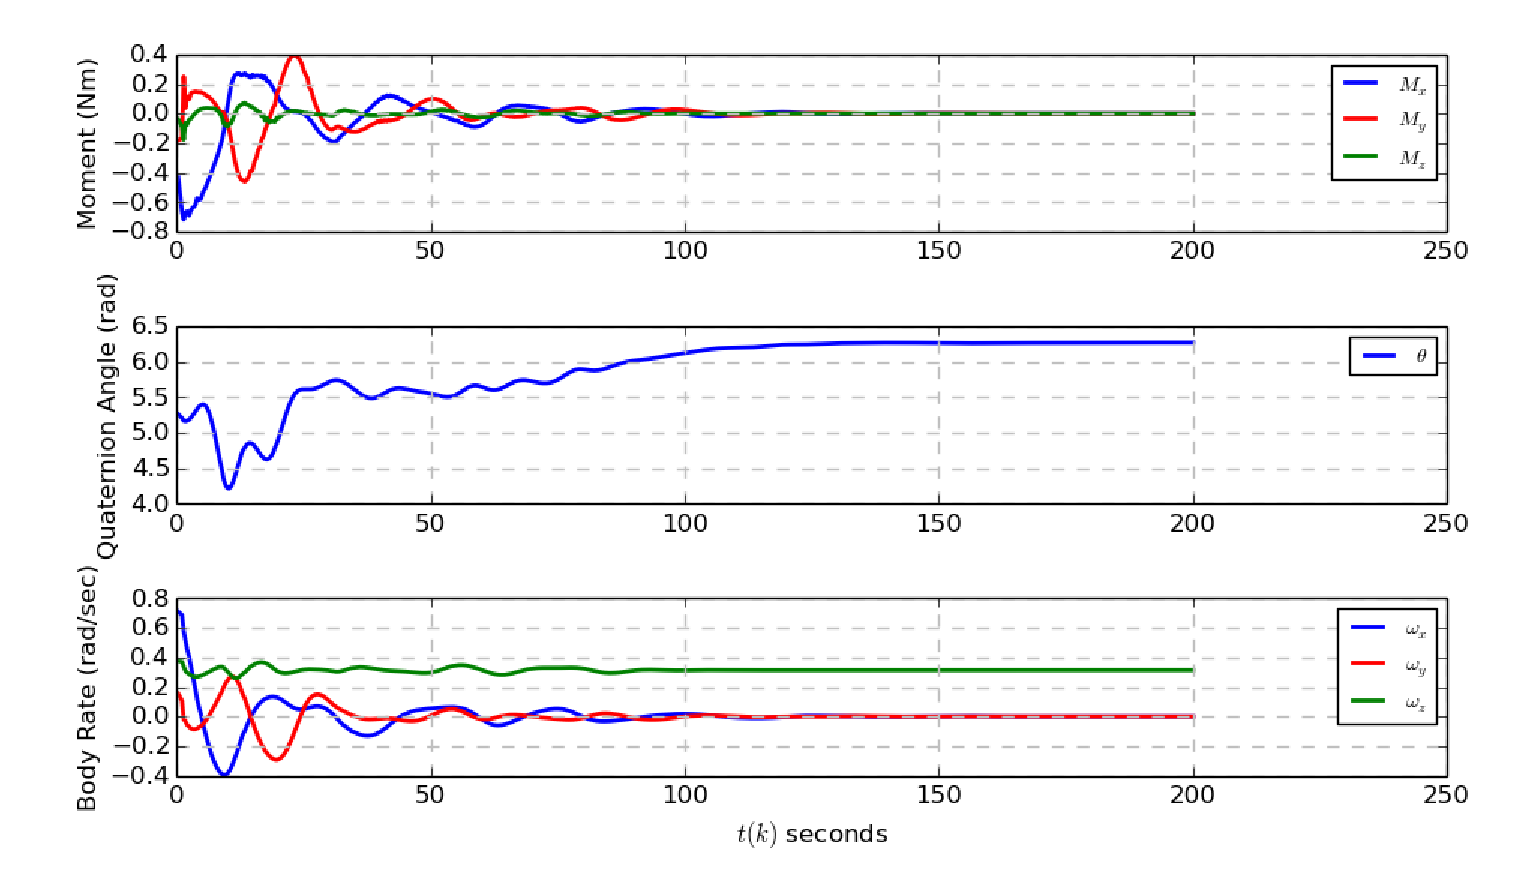
\psfig{file=figures/pid_attitude_and_rate_control.eps,width=6in}}
  \caption{PID Attitude and Rate Control}
  \label{fig:PIDAttitudeAndRateControl}
\end{figure}
Figure \ref{fig:PIDAttitudeAndRateControl} shows a significant improvement in the body rate control response over previous body rate tests.  All error and oscillations in the quaternion angle are also eliminated.  The proportional, integral, and derivative terms that comprise the moment value from Figure \ref{fig:PIDAttitudeAndRateControl} are shown individually in Figure \ref{fig:PIDAttitudeAndRateControlMoments}.
\begin{figure}[H]
  \centerline{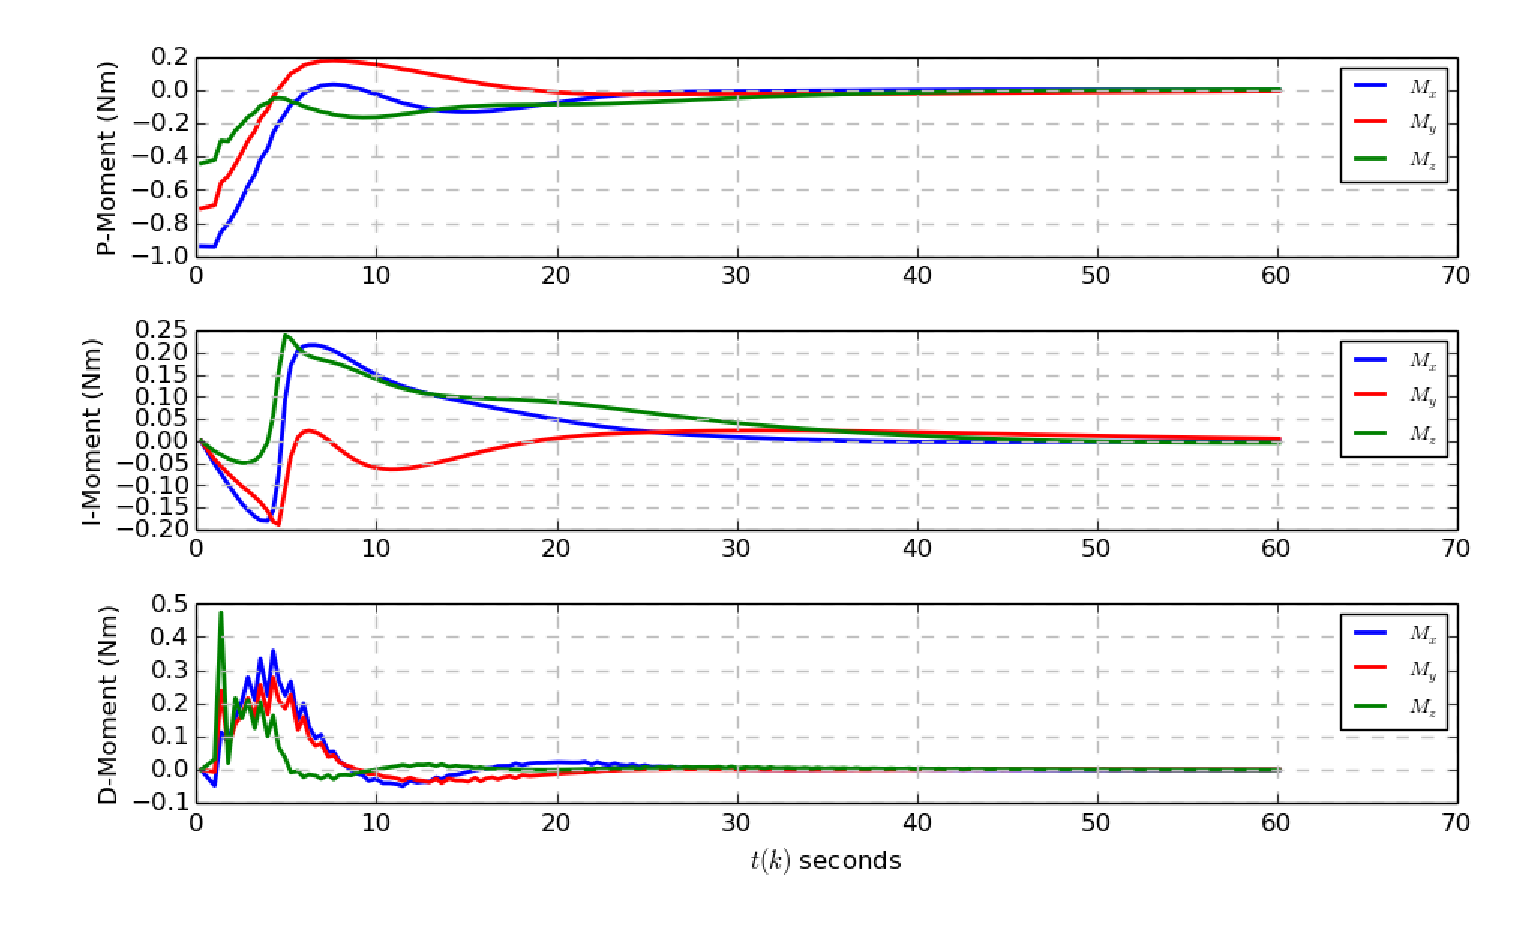
\psfig{file=figures/pid_attitude_and_rate_control_moments.eps,width=6in}}
  \caption{PID Attitude and Rate Control Moments}
  \label{fig:PIDAttitudeAndRateControlMoments}
\end{figure}

The Sliding Mode Controller is designed such that
\begin{equation}
  \begin{aligned}
    \bs{M} &= \bs{M}_{q} + \bs{M}_{\omega} \\
    \bs{M}_{q} &= \left[- L_{q} \cos^{-1} (q_{0e}) \right] \bs{\hat{e}}_e + \left[ K_{q} sat \left( \frac{-2\cos^{-1} (q_{0e})}{S_q} \right) \right] \bs{\hat{e}}_e \\
    \bs{M}_{\omega} &= \bs{L}_{\omega} \bs{\omega}_e + \bs{K}_{\omega}\bs{1}_s \big(\bs{\omega}_e / S_{\omega} \big) \\
    \bs{1}_s \big(\bs{\omega}_e / S_{\omega} \big) &= \begin{bmatrix} sat (\omega_{ex} / S_{\omega}) &0 &0 \\ 0 & sat (\omega_{ey} / S_{\omega}) & 0 \\ 0 & 0 & sat (\omega_{ez} / S_{\omega}) \end{bmatrix}
  \end{aligned}
  \label{eqn:sliding_mode_control}
\end{equation}
Where $S_{\omega}$ represents the boundary layer for the saturation functions.

Figures \ref{fig:SMCAttitudeAndRateControl} and \ref{fig:SMCAttitudeAndRateControlMoments} show the response of the SMC for attitude and body rate control.  Through a gradient descent search, the SMC parameters are tuned to
\begin{equation}
  \begin{aligned}
    L_q &= 0.408, \bs{L}_{\omega} = \bs{I} \begin{bmatrix} 0.708 & 0.678 & 0.525 \end{bmatrix}^T \\
    K_q &= 0.500, \bs{K}_{\omega} = \bs{I} \begin{bmatrix} 0.745 & 0.816 & 0.666 \end{bmatrix}^T \\
    S_q &= 0.607, S_{\omega} = 0.315
  \end{aligned}
\end{equation}
\begin{figure}[H]
  \centerline{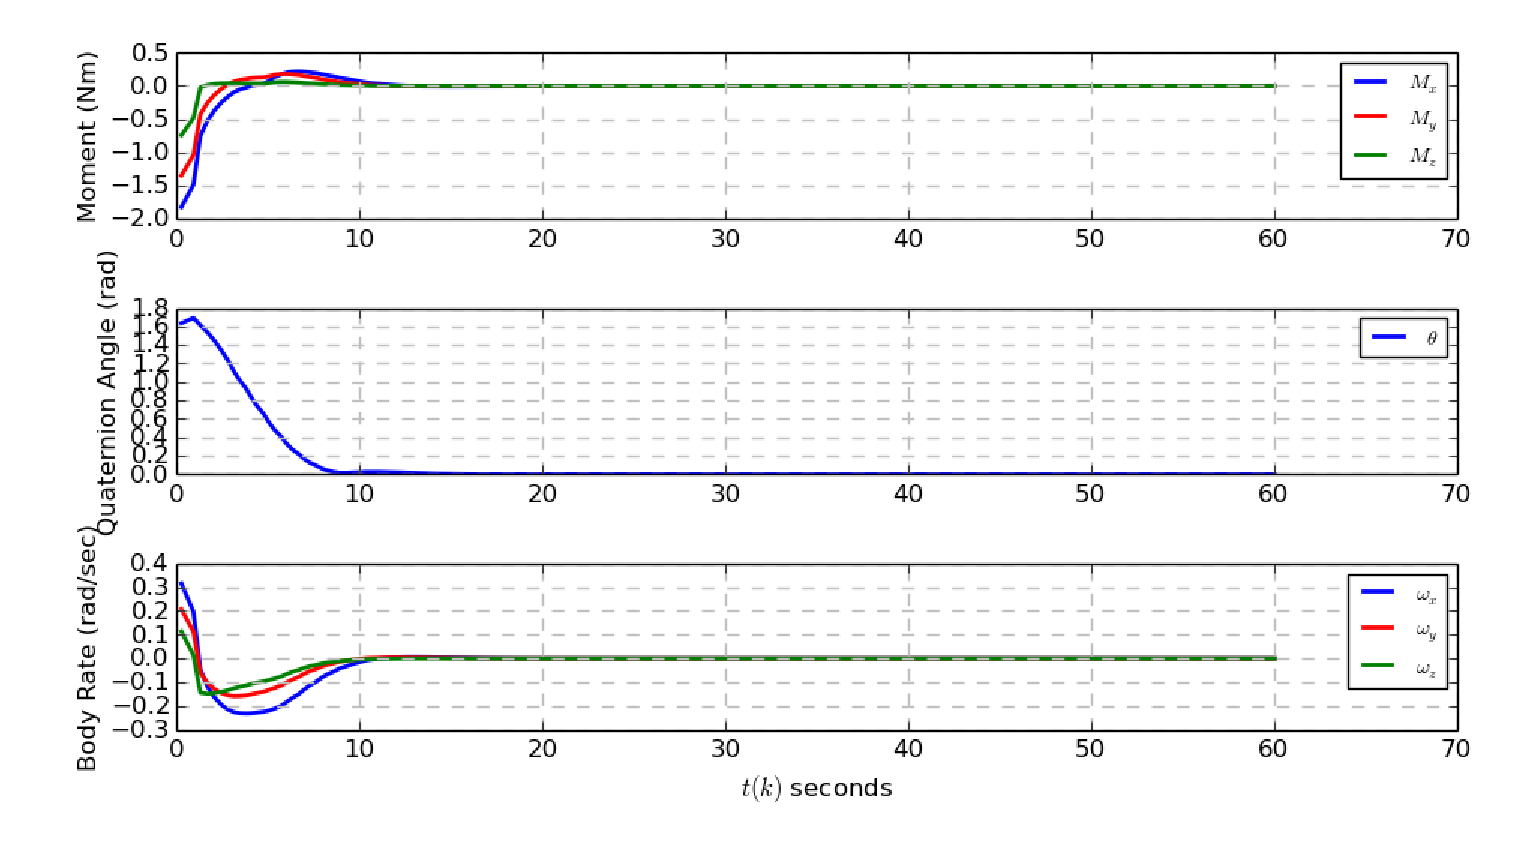
\psfig{file=figures/smc_attitude_and_rate_control.eps,width=6in}}
  \caption{SMC Attitude and Rate Control}
  \label{fig:SMCAttitudeAndRateControl}
\end{figure}
\begin{figure}[H]
  \centerline{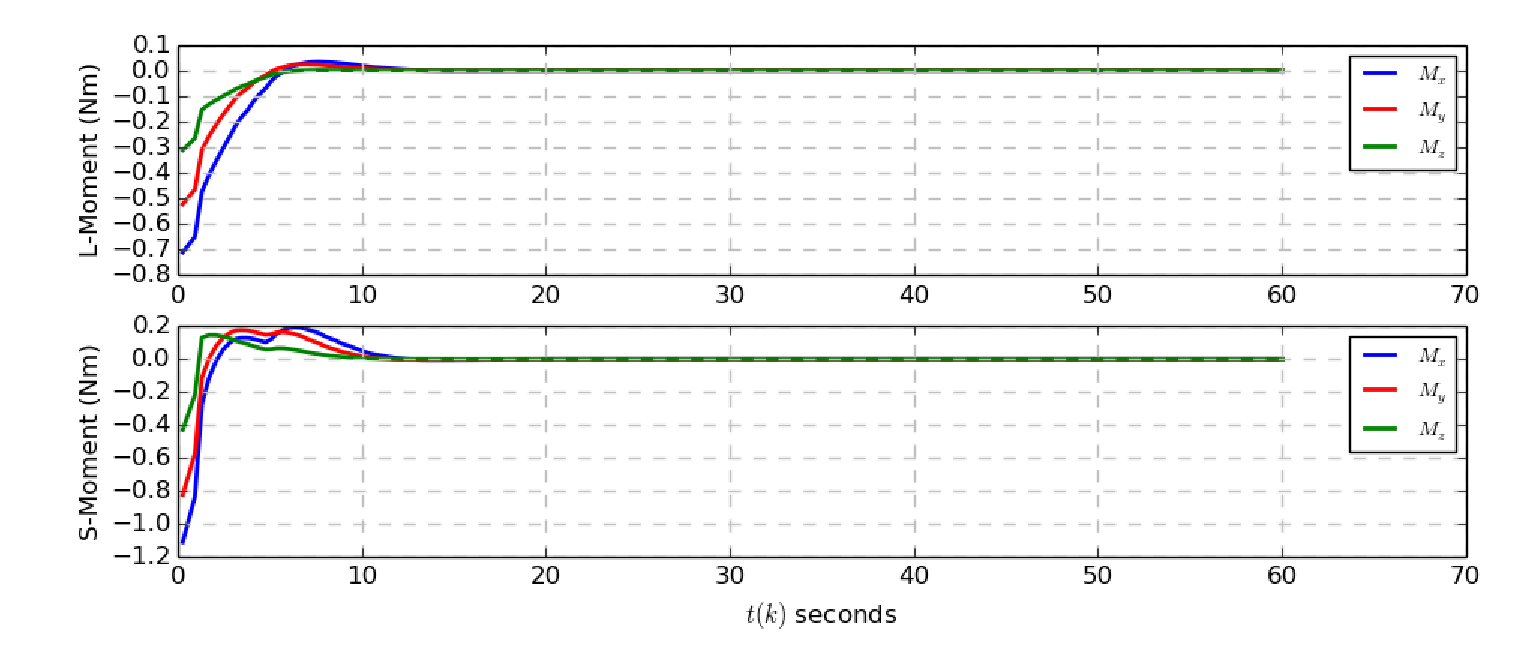
\psfig{file=figures/smc_attitude_and_rate_control_moments.eps,width=6in}}
  \caption{SMC Attitude and Rate Control Moments}
  \label{fig:SMCAttitudeAndRateControlMoments}
\end{figure}
As with the body rate comparative tests, the SMC shows a significant improvement in performance compared to the PID controller for fixed attitude and body control.

\subsection{Spin-Stabilized Control}
\label{subsec:SpinStabilizedControl}

For the fixed attitude control problem from Section (\ref{subsec:FixedAttitudeControl}), this section verifies the ability of a controller to release the quaternion restriction on the rotational attitude leaving the system to control five degrees of freedom: $\omega_z = 0.314, \omega_x = \omega_y = 0$ and zero nutation about the $x$ and $y$ axes.  Since the Sliding Mode Controller regularly out performs the PID controller, the spin-stabilized controller will run with control Equation (\ref{eqn:sliding_mode_control}) using the following controller gains:
\begin{equation}
  \begin{aligned}
    L_q &= 0.01, \bs{L}_{\omega} = \bs{I} \begin{bmatrix} 0.398 & 0.383 & 0.416 \end{bmatrix}^T \\
    K_q &= 0.01, \bs{K}_{\omega} = \bs{I} \begin{bmatrix} 0.440 & 0.510 & 0.316 \end{bmatrix}^T \\
    S_q &= 0.01, S_{\omega} = 0.140
  \end{aligned}
\end{equation}

The initial convergence of the spin-stabilized state takes place quickly, as in previous test configurations.  In this case, however, the controller is not able to fully remove the attitude error.  Additional gain tuning or the inclusion of advanced visualizations such as the tPlot discussed in Section \ref{sec:ObjectOrientedNSSControlSystem} is required to diagnose the source of the error.
\begin{figure}[H]
  \centerline{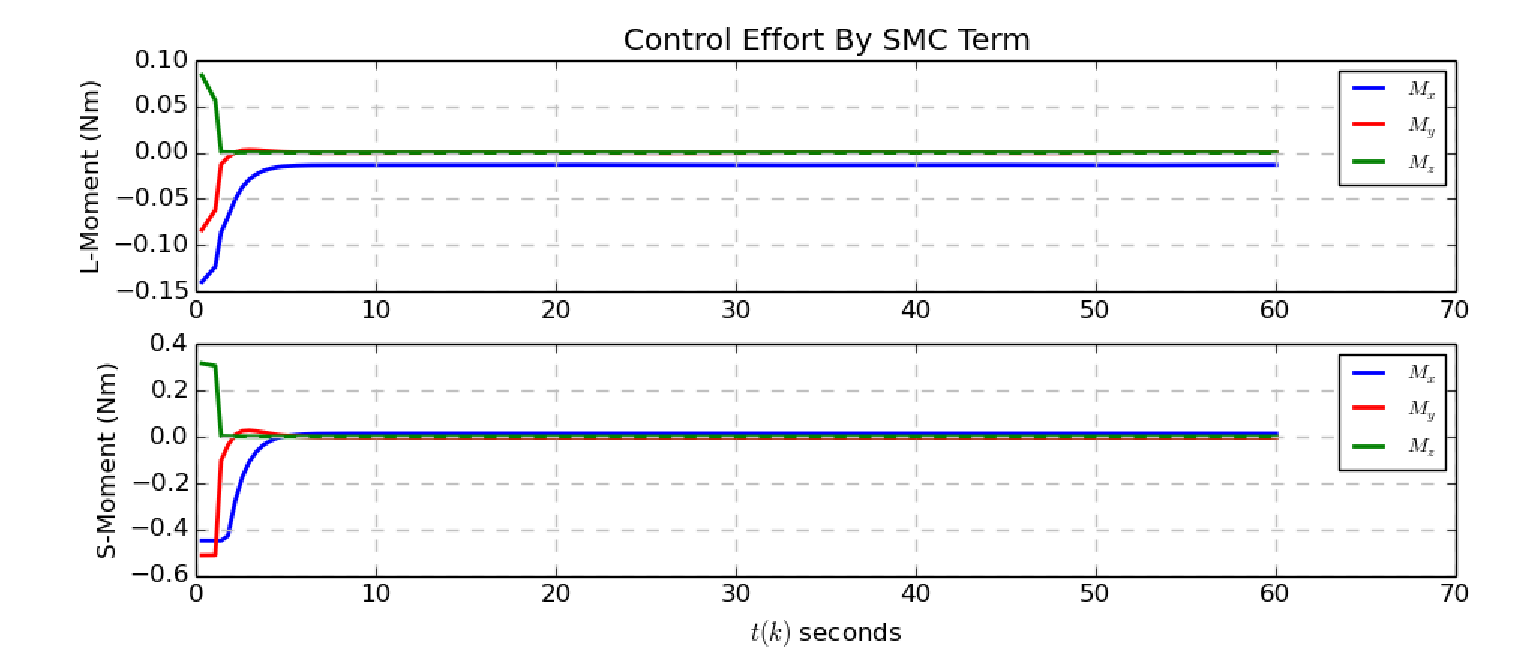
\psfig{file=figures/smc_nutation_and_rate_control.eps,width=6in}}
  \caption{SMC Nutation and Rate Control}
  \label{fig:SMCNutationAndRateControl}
\end{figure}
\begin{figure}[H]
  \centerline{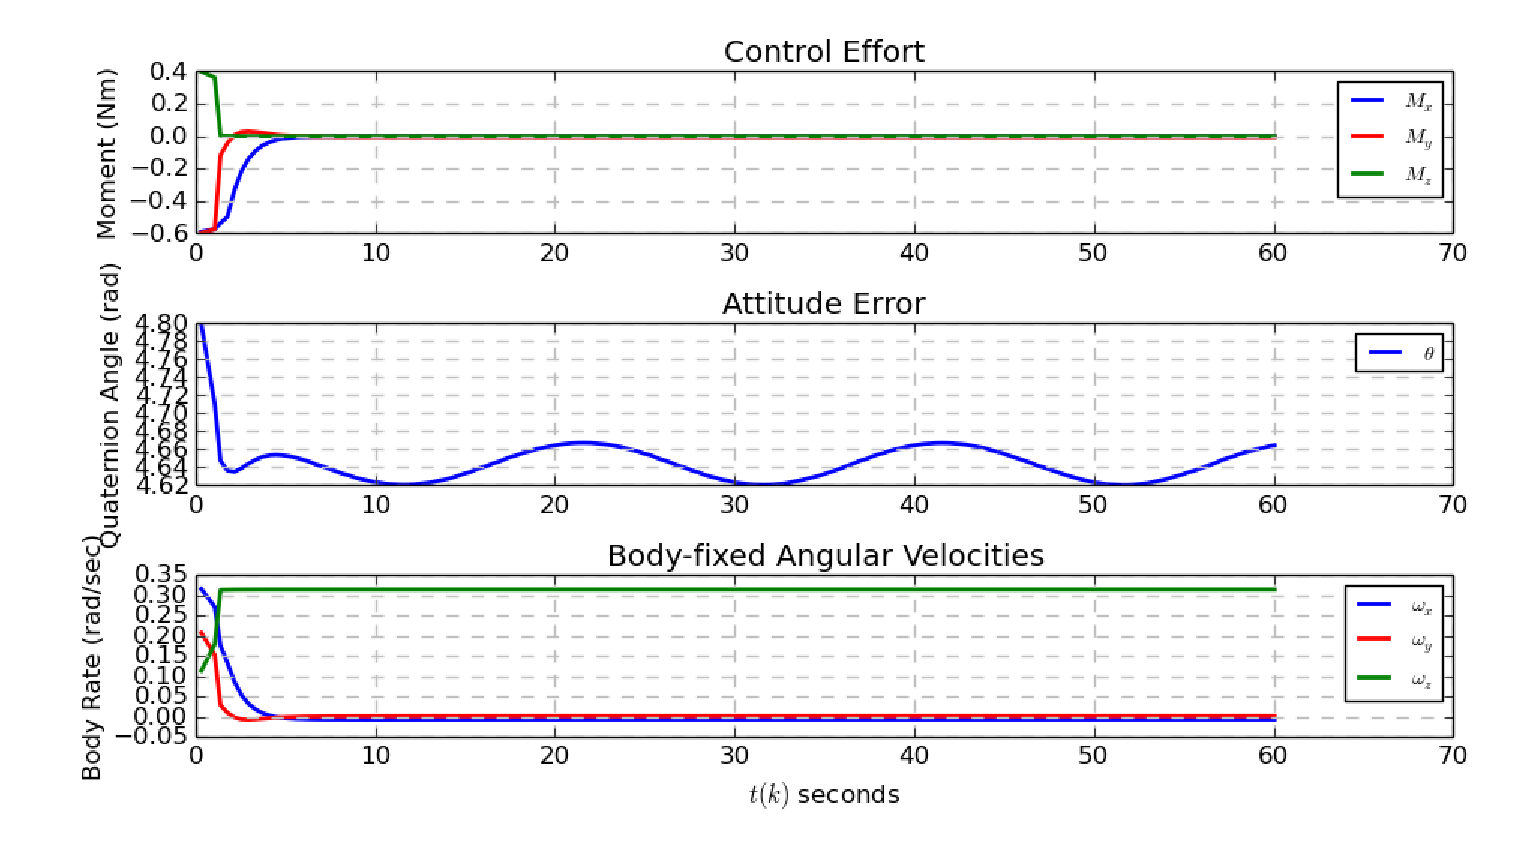
\psfig{file=figures/smc_nutation_and_rate_control_moments.eps,width=6in}}
  \caption{SMC Nutation and Rate Control Moments}
  \label{fig:SMCNutationAndRateControlMoments}
\end{figure}


\chapter{OBSERVER BASED CONTROLS}
\label{chap:ObserverBasedControls}

Chapter \ref{chap:UNHTableSat1A} detailed how TableSat's sensor readings could be quantified and represented in terms of engineering units.  Chapter \ref{chap:SatelliteAttitudeModeling} established the state representation of the system and the chosen dynamic equations used to model it's behavior.  This chapter will focus on the estimation techniques to improve the accuracy of the state representations, and control techniques to guide the system into the desired state.

\section{State Error}
\label{sec:StateError}

In both the estimation and control techniques, a process for determining how close two states are from each other is required.  For the estimation case,  the error $\bs{\hat{x}}_e$ between the measured state $\bs{x}$ and the estimated state $\bs{\hat{x}}$.  For the controllers, the state error $\bs{x}_e$ representing the offset between the estimated state $\bs{\hat{x}}$ and the desired state $\bs{x}_d$.

\begin{subequations}
  \begin{align}
    \bs{\hat{x}}_e &= \bs{\hat{x}} - \bs{x} \\
    \bs{x}_e &= \bs{\hat{x}} - \bs{x}_d
  \end{align}
  \label{eqn:StateError}
\end{subequations}

Multiple methods were used to quantify the differences in states.  For comparison and to demonstrate their use with TSatPy, the following sections will limit its focus on a single update of proportional estimator.

\begin{equation}
  \bs{\hat{x}(t_{k+1})} = \bs{\hat{x}}(t_{k}) + \bs{K_p} ( \bs{\hat{x}}(t_{k}) - \bs{x}(t_{k}) )
  \label{eqn:PEstimatorStateDiff}
\end{equation}

This simple estimation technique has some notable deficiencies when applied to the attitude parameters of a spin stabilized satellite.  These parameters are expected to change as the satellite rotates, but this model has no method for predicting the change in parameters so will rely solely on the state error to correct $\bs{\hat{x}(t_{k+1})}$.  After an adequate method is established for calculating the state error, later sections will address improving upon the proportional estimator.

The sample error calculation in this section will be based off a last estimated state, $\bs{\hat{x}}(t_{k})$, of a $190^o$ rotation about $+z$-axis and a body rate of $\omega_z = 3$ rad/sec.  The associated the measured state, $\bs{x}(t_{k})$, is a $44^o$ rotation about the axis $0 \bs{i} + 0.1 \bs{j} + 1\bs{k}$ and a body rate of $\omega_z = 3.1$ rad/sec.


\begin{subequations}
  \begin{align}
    \bs{\hat{x}}(t_{k})
    = \begin{bmatrix}  \bs{\hat{q}}(t_{k}) \\ \bs{\hat{\omega}}(t_{k}) \end{bmatrix}
    &= \begin{bmatrix} 0 \bs{i} +0 \bs{j} -0.996195 \bs{k} -0.0871557 \\ 0 \bs{i} +0 \bs{j} +3 \bs{k} \end{bmatrix}\\
    \bs{x}(t_{k})
    = \begin{bmatrix}  \bs{q}(t_{k}) \\ \bs{\omega}(t_{k}) \end{bmatrix}
    &= \begin{bmatrix} 0 \bs{i} -0.0372747 \bs{j} -0.372747 \bs{k} +0.927184 \\ 0 \bs{i} +0 \bs{j} +3.1 \bs{k} \end{bmatrix}
  \end{align}
  \label{eqn:StateDifferenceQuaternionSamples}
\end{subequations}

\begin{singlespace}
  \begin{minted}[mathescape,linenos,numbersep=10pt,frame=lines,framesep=2mm]{python}
from TSatPy.State import Quaternion, QuaternionError, State, BodyRate
import numpy as np

x_hat = State(
    Quaternion([0,0,1],radians=190/180.0*np.pi),
    BodyRate([0,0,3]))
x_m = State(
    Quaternion([0,0.1,1],radians=44/180.0*np.pi),
    BodyRate([0,0,3.1]))
print("x_hat:  %s" % (x_hat))
print("x_m:    %s" % (x_m))

# Prints Out
# x_hat:  <Quaternion [-0 -0 -0.996195], -0.0871557>,
#         <BodyRate [0 0 3]>
# x_m:    <Quaternion [-0 -0.0372747 -0.372747], 0.927184>,
#         <BodyRate [0 0 3.1]>
  \end{minted}
\nocite{minted}
\end{singlespace}

Section \ref{subsec:StateDifference} will start out with the standard element wise matrix difference to represent the state error.

\subsection{State Difference}
\label{subsec:StateDifference}

The standard method for calculating the state error in either an estimation or control method is to calculate an element-wise difference.  TableSat has a seven element state in matrix form and expanding Equation \ref{eqn:StateError} becomes

\begin{equation}
  \begin{aligned}
    \bs{\hat{x}}_e(t_{k}) &= \begin{bmatrix}  \bs{\hat{q}}_e(t_{k}) \\ \bs{\hat{\omega}}_e(t_{k}) \\ \end{bmatrix} \\
    &= \begin{bmatrix} (\hat{q}_1 - q_{1}) \bs{i} + (\hat{q}_2 - q_{2}) \bs{j} + (\hat{q}_3 - q_{3}) \bs{k} + \hat{q}_0 - q_{0} \\ (\hat{\omega}_x - \omega_{x}) \bs{i} + (\hat{\omega}_y - \omega_{y}) \bs{j} + (\hat{\omega}_z - \omega_{z}) \bs{k} \end{bmatrix}
  \end{aligned}
  \label{eqn:StateDifference}
\end{equation}


Calculating the difference between the example estimated and measured states in Equation \ref{eqn:StateDifferenceQuaternionSamples} yields a state difference of

\begin{equation}
  \begin{aligned}
    \bs{\hat{x}}_e(t_{k})
    = \begin{bmatrix}  \bs{\hat{q}}_e(t_{k}) \\ \bs{\hat{\omega}}_e(t_{k}) \end{bmatrix}
    &= \begin{bmatrix} 0 \bs{i} +0.0372747 \bs{j} -0.623447 \bs{k} -1.01434 \\ 0 \bs{i} +0 \bs{j} -0.1 \bs{k} \end{bmatrix}
  \end{aligned}
  \label{eqn:StateDifferenceSample}
\end{equation}


\begin{singlespace}
  \begin{minted}[mathescape,linenos,numbersep=10pt,frame=lines,framesep=2mm]{python}
x_e = State(
    Quaternion(x_hat.q.vector - x_m.q.vector,
        x_hat.q.scalar - x_m.q.scalar),
    x_hat.w - x_m.w)
print("x_e:  %s" % (x_e))

# Prints Out
# x_e:  <Quaternion [0 0.0372747 -0.623447], -1.01434>,
#       <BodyRate [0 0 -0.1]>
  \end{minted}
\nocite{minted}
\end{singlespace}


The body rate error calculations are well behaved and are able to be directly used with standard estimation based control techniques.  The difference in quaternion parameters however pose a number of problems even when used in a basic proportional estimator.  Using this method of error measurement will be difficult especially since after a cursory review the scalar quantity in the error quaternion that is outside the possible range for a rotational quaternion.  Section \ref{subsec:QuaternionDifferencebasedPEstimator} will attempt to use this state difference along with a standard proportional estimation technique.

\subsection{Quaternion Difference based P-Estimator}
\label{subsec:QuaternionDifferencebasedPEstimator}

Taking the quaternion difference from Equation \ref{eqn:StateDifferenceSample}, and incorporating into the proportional estimation correction in Equation \ref{eqn:PEstimatorStateDiff} produces an state adjustment and estimated attitude of

\begin{equation}
  \begin{aligned}
    \bs{q}_{adj} = -0.8 \cdot \bs{q}_e =& -0.8 \cdot (0 \bs{i} + 0.0372747 \bs{j} -0.623447 \bs{k} -1.01434 ) \\
                       =& 0 \bs{i} -0.0298198 \bs{j} +0.498758 \bs{k} +0.811472 \\
    \bs{\hat{q}(t_{k+1})} =& \bs{\hat{q}(t_{k})} + \bs{q}_{adj} \\
                       =& 0 \bs{i} -0.0298198 \bs{j} -0.497437 \bs{k} + 0.724316 \\
  \end{aligned}
\end{equation}

\begin{singlespace}
  \begin{minted}[mathescape,linenos,numbersep=10pt,frame=lines,framesep=2mm]{python}
q_hat = x_hat.q
q_e = x_e.q
q_adj = Quaternion(-0.8 * q_e.vector, -0.8 * q_e.scalar)
q_hat_new = Quaternion(q_hat.vector + q_adj.vector,
        q_hat.scalar + q_adj.scalar)

print("q_e:         %s" % (q_e))
print("q_adj:       %s" % (q_adj))
print("q_hat_new:   %s" % (q_hat_new))
print("|q_hat_new|: %g" % (q_hat_new.mag))

# Prints Out
# q_e:         <Quaternion [0 0.0372747 -0.623447], -1.01434>
# q_adj:       <Quaternion [-0 -0.0298198 0.498758], 0.811472>
# q_hat_new:   <Quaternion [-0 -0.0298198 -0.497437], 0.724316>
# |q_hat_new|: 0.879185
  \end{minted}
\nocite{minted}
\end{singlespace}

The new estimate for the quaternion attitude has been adjusted closer to the measured state although the newly estimated state has a norm of $ \| \bs{\hat{q}(t_{k+1})} \| = 0.879185$.  Since failing to conform to the unit magnitude for rotational quaternions, this newly estimated attitude quaternion corrupts the systems state especially over multiple steps and long simulations.  For rotational quaternions with norms less that the unit quaternion the rotated points end up converging into the origin.  If the adjustment ends up with a rotational quaternion larger than a unit magnitude, rotated points dilate away from the origin.

\begin{singlespace}
  \begin{minted}[mathescape,linenos,numbersep=10pt,frame=lines,framesep=2mm]{python}
pt = np.mat([[1,0,0]])
pt = q_hat_new.rotate_points(pt)
print("pt * pt.T:   %s" % (pt * pt.T))

# Prints Out
# pt * pt.T:   [[ 0.5974769]]
  \end{minted}
\nocite{minted}
\end{singlespace}


\subsection{Scaled Quaternion Difference based P-Estimator}
\label{sec:ScaledQuaternionDifferencebasedPEstimator}

The next step to correct for the dilation or compression of points is to scale the adjusted quaternion to a unit quaternion before using it to represent the system's state.  The quaternion can be scaled through a standard vector normalization.

\begin{equation}
  \bs{\hat{q}}_n = \frac{\bs{q}_v + q_0}{\sqrt{\bs{q}_v \bullet \bs{q}_v + q_0^2}}
  \label{eqn:NormalizeQuaternion}
\end{equation}

\begin{singlespace}
  \begin{minted}[mathescape,linenos,numbersep=10pt,frame=lines,framesep=2mm]{python}
print("q_hat_new:   %s" % (q_hat_new))
q_hat_new.normalize()
print("q_hat_new:   %s" % (q_hat_new))
print("|q_hat_new|: %g" % (q_hat_new.mag))

# Prints Out
# q_hat_new:   <Quaternion [-0 -0.0298198 -0.497437], 0.724316>
# q_hat_new:   <Quaternion [-0 -0.0339175 -0.565793], 0.823849>
# |q_hat_new|: 1
  \end{minted}
\nocite{minted}
\end{singlespace}

The newly estimated state is equivalent to a $69$ degree rotation about
\begin{equation}\hat{\bs{e}} = \begin{bmatrix} 0 & -0.0598395 & -0.998208 \end{bmatrix}\end{equation}.  While this state estimate conforms to the unit quaternion requirement and will no longer corrupt rotations, it has little in common with the desired $0.8$ proportional gain used the estimator's design.

\begin{singlespace}
  \begin{minted}[mathescape,linenos,numbersep=10pt,frame=lines,framesep=2mm]{python}
e, r = q_hat_new.to_rotation()
print("e: <%g, %g, %g>\ndegree: %g" % (
    e[0,0],e[1,0],e[2,0], r * 180.0 / np.pi))

# Prints Out
# e: <-0, -0.0598395, -0.998208>
# degree: 69.056
  \end{minted}
\nocite{minted}
\end{singlespace}


\subsection{Quaternion Multiplicative Correction}
\label{subsec:QuaternionMultiplicativeCorrection}

The previous sections have established that the state difference approach for adjusting for errors in attitude measurements has significant issues especially for low frequency updates with high error values.  The quaternion multiplication defined in Equation \ref{eqn:QuaternionMultiplication} can be used to modify the attitude while not introducing corruption into the model if used with rotational unit quaternions.

If the estimated and measured states converge with the multiplicative correction, the error quaternion should converge to the identity quaternion.  The identity quaternion as with the identity matrix is the quantity that when multiplied by another quaternion, does not modify its value.  This identity holds true for general as well as rotational quaternions.

\begin{equation}
  \bs{q}_I = 0 \bs{i} + 0 \bs{j} + 0 \bs{k} + 1
\end{equation}

An Identity function was created it the TSatPy.State module to construct an identity quaternion.

\begin{singlespace}
  \begin{minted}[mathescape,linenos,numbersep=10pt,frame=lines,framesep=2mm]{python}
from TSatPy import State

q = State.Quaternion([1,2,3], 4)
print("q       = %s" % q)
q_I = State.Identity()
print("q_I     = %s" % q_I)
print("q_I * q = %s" % (q_I * q))

# Prints Out
# q       = <Quaternion [1 2 3], 4>
# q_I     = <Quaternion [0 0 0], 1>
# q_I * q = <Quaternion [1 2 3], 4>
  \end{minted}
  \nocite{minted}
\end{singlespace}

Rotational quaternions are considered equal if they represent the same attitude.  The same attitude can be represented by more than one distinct quaternions, so a strict equality is not adequate.  The test for equality can be done by using the quaternion conjugate $\bs{q}^*$.

\begin{subequations}
  \begin{align}
    \bs{\hat{q}} = \bs{q} & \iff \bs{\hat{q}}^* \otimes \bs{q} = \bs{q}^* \otimes \bs{\hat{q}} = \bs{q}_I \text{ or } -\bs{q}_I \\
    \text{where } \bs{q}^* &= \begin{bmatrix} -\bs{v} \\ q_0 \end{bmatrix}
  \end{align}
  \label{eqn:QuaternionEquality}
\end{subequations}

The sample below shows how two distinct quaternions can represent the same attitude and that Equation \ref{eqn:QuaternionEquality} holds true.

\begin{singlespace}
  \begin{minted}[mathescape,linenos,numbersep=10pt,frame=lines,framesep=2mm]{python}
a = Quaternion([0,0,1],radians=190/180.0*np.pi)
b = Quaternion([0,0,1],radians=(190 + 360)/180.0*np.pi)

print("a:          %s" % (a))
print("b:          %s" % (b))
print("a.conj * b: %s" % (a.conj * b))

# Prints Out
# a:          <Quaternion [-0 -0 -0.996195], -0.0871557>
# b:          <Quaternion [0 0 0.996195], 0.0871557>
# a.conj * b: <Quaternion [0 0 -3.46945e-16], -1>
  \end{minted}
\nocite{minted}
\end{singlespace}

Equation \ref{eqn:QuaternionEquality} provides a method for determining whether two quaternions represent the same attitude, it can also be used to quantify the difference between two rotational quaternions using the multiplicative comparison.

\begin{equation}
  \bs{q}_e = \bs{q}^* \otimes \bs{\hat{q}}
  \label{eqn:QuaternionError}
\end{equation}

Continuing with the example measured and estimated states from Equation \ref{eqn:StateDifferenceQuaternionSamples}, the multiplicative quaternion error between these states evaluates to

\begin{equation}
  \begin{aligned}
    \bs{q}_e = & \bs{q}^* \otimes \bs{\hat{q}} \\
    = & \big( 0 \bs{i} -0.0372747 \bs{j} -0.372747 \bs{k} +0.927184 \big)^* \\
    & \otimes \big( 0 \bs{i} +0 \bs{j} -0.996195 \bs{k} -0.0871557 \big)\\
    = & -0.0371329 \bs{i} -0.00324871 \bs{j} -0.956143 \bs{k} +0.29052
  \end{aligned}
  \label{eqn:QuaternionErrorSample}
\end{equation}

The sample error measurement in Equation \ref{eqn:QuaternionErrorSample} relates well to the deviations in the estimated and measured attitudes as it represents a 146 degree rotation about the Euler axis $<-0.0388067, -0.00339514, -0.999241>$ which would rotate the estimated quaternion back to match up perfectly with the measured state.  The multiplicative error correction quaternion also solves the issue encountered in Section \ref{subsec:QuaternionDifferencebasedPEstimator} where the magnitude of the error quaternion did not remain fixed at the unit quaternion.

\begin{singlespace}
  \begin{minted}[mathescape,linenos,numbersep=10pt,frame=lines,framesep=2mm]{python}
from TSatPy.State import QuaternionError
q_e = QuaternionError(x_hat.q, x_m.q)

print("q_e:   %s" % (q_e))
print("|q_e|: %s" % (q_e.mag))
e, r = q_e.to_rotation()
print("e:     <%g, %g, %g>\ndegree: %g" % (
    e[0,0],e[1,0],e[2,0], r * 180.0 / np.pi))

# Prints Out
# q_e:   <Quaternion [-0.0371329 -0.00324871 -0.956143], 0.29052>
# |q_e|: 1.0
# e:     <-0.0388067, -0.00339514, -0.999241>
# degree: 146.222
  \end{minted}
\nocite{minted}
\end{singlespace}

\subsection{Quaternion Multiplicative Correction P-Estimation}
\label{subsec:QuaternionMultiplicativeCorrectionPEstimation}

Section \ref{subsec:QuaternionMultiplicativeCorrection} was able to establish a method for quantifying differences in attitudes in a method that preserves the integrity of the rotational quaternion while creating a representative measure of the state error.  For the next step, a series of options were investigated to determine how the error measurement can be used in estimation and control techniques.

\subsubsection{Parameter Multiplier}
\label{subsubsec:ParameterMultiplier}

With a parameter multiplier method, the four parameters of the error quaternion get scaled by a $\bs{K_p}$ term similar to the standard proportional adjustment.

\begin{equation}
  \bs{q}_{adj} = \bs{K_p} \bs{q}_e
    = \bs{K_p} \begin{bmatrix} \bs{v}_e \\ q_{e0} \end{bmatrix}
    = \begin{bmatrix} \bs{K_{vp}}\bs{v}_e \\ K_{0p} \cdot q_{e0} \end{bmatrix}
  \label{eqn:ParameterMultiplier}
\end{equation}

The $\bs{K_{vp}}$ term is a 3x3 matrix.  Since $\bs{v}_e$ defines the path between the estimated and measured quaternions the only form of $\bs{K_{vp}}$ that would not corrupt the direction mapped between the two states is

\begin{equation}
  \bs{K_{vp}} \bs{v}_e = \lambda \bs{v}_e
  \label{eqn:QuaternionVectorCorrection}
\end{equation}

The effect of the $\lambda$ parameter is to modify the magnitude of the quaternion's Euler axis but not modify it's direction.  Combining \ref{eqn:QuaternionVectorCorrection} with \ref{eqn:ParameterMultiplier} yields

\begin{equation}
  \bs{q}_{adj} = \begin{bmatrix} \lambda \bs{v}_e \\ K_{0p} \cdot q_{e0} \end{bmatrix}
  \label{eqn:QuaternionScalarMultiplier}
\end{equation}

Reducing the tunable parameters for the proportional quaternion estimator to $\lambda$ and $K_{0p}$.  This configuration, shares the same flaws as the state difference approach in Section \ref{subsec:QuaternionDifferencebasedPEstimator} where the magnitude of the adjusted quaternion can vary from the unit quaternion causing dilation or compression of rotated points.

\begin{singlespace}
  \begin{minted}[mathescape,linenos,numbersep=10pt,frame=lines,framesep=2mm]{python}
q_adj = Quaternion(
    q_e.vector * 0.7,  # lambda chosen as 0.7
    q_e.scalar * 0.4)  # K_p0 chosen as 0.4

print("q_adj:   %s" % (q_adj))
print("|q_adj|: %s" % (q_adj.mag))

# Prints Out
# q_adj:   <Quaternion [-0.025993 -0.0022741 -0.6693], 0.116208>
# |q_adj|: 0.679814272084
  \end{minted}
\nocite{minted}
\end{singlespace}


\subsubsection{Normalized Parameter Multiplier}
\label{subsubsec:NormalizedParameterMultiplier}

Normalizing the paramater multiplier's adjustment quaternion resolves the issues with dilating and contracting points as it did in Section \ref{sec:ScaledQuaternionDifferencebasedPEstimator}.  A normalized parameter multiplier quaternion does not suffer from an invalid Euler axis of rotation as in Section \ref{sec:ScaledQuaternionDifferencebasedPEstimator} as only the magnitude of the quaternion's vector is modified.  The scalar quantity however still ends up being muddied due to the coupling between  and $K_{0p}$ that occurs via normalization.  A constant angular error and $K_{0p}$ can create varied adjustment values based on the selection of the $\lambda$ gain.

\subsubsection{Scalar Multiplier with Normalization}
\label{subsubsec:ScalarMultiplierWithNormalization}

Since the $\lambda$ gain used above provides no benefit and only ends up complicating the quaternion adjustment calculation, it can be dropped leaving a quaternion adjustment based solely on a modification of the scalar quantity.  After the scalar gain $k$, the quaternion can be normalized back to a unit quaternion.

\begin{equation}
  \begin{aligned}
  \bs{q}_{adj} = & \begin{bmatrix} \bs{v}_e / \alpha \\ ( k \cdot q_{e0} )  / \alpha \end{bmatrix} \\
  \text{where } \alpha & = \sqrt{\bs{v}_e^T \cdot \bs{v}_e + k^2 \cdot q_{e0}^2}
  \end{aligned}
  \label{eqn:ScalarMultiplierWithNormalization}
\end{equation}

Equation \ref{eqn:ScalarMultiplierWithNormalization} has a few strengths when used to apply adjustments to a quaternion attitude estimate.  It's based off the multiplicative correction quaternion that accurately quantifies the difference in estimated and measured states.  The normalization ensures that the rotational quaternion representation is not corrupted and when applied will not cause dilation or compression of the model.

The disadvantage to using this representation is that the quaternion scalar parameter is a nonlinear function of the rotation angle (Equation \ref{eqn:RotationalQuaternionDefinition}).  Applying a constant scalar multiplier to it will result in inconsistent adjustment amount depending on the position along the sinusoidal value.

\subsubsection{Angle Multiplier with Vector Magnitude Normalization}
\label{subsubsec:AngleMultiplierWithVectorMagnitudeNormalization}

The section will cover the final version of the quaternion adjustment calculation that takes into consideration all the issues encountered in the above sections.  The function designated in this thesis for the scaling of a quaternion to for use with quaternion multiplicative corrections while maintaining it's connection to the physical system will be $\bs{\psi}(\bs{q}, k)$ where

\begin{equation}
  \begin{aligned}
    \bs{\psi}(\bs{q}, k) &= \begin{bmatrix} \bs{v} / \gamma \\ \cos ( k \cdot \cos^{-1} (q_0))  \end{bmatrix} \\
    \text{where } \gamma &= \sqrt{\frac{\bs{v}^T \cdot \bs{v}}{\sin^2 ( k \cdot \cos^{-1} (q_0))}} \\
    \bs{q} &= \begin{bmatrix} \bs{v} \\ q_0  \end{bmatrix}
  \end{aligned}
  \label{eqn:PSI}
\end{equation}

Using Equation \ref{eqn:PSI} to create a rotational quaternion adjustment for the proportional estimator would take the form.

\begin{equation}
  \bs{q}_{adj} = \bs{\psi}(\bs{q}_e, k)
  \label{eqn:PEstimatorAngleMultiplierwithVectorMagnitudeNormalization}
\end{equation}

The code snippet below demonstrates the usage of Equation \ref{eqn:PEstimatorAngleMultiplierwithVectorMagnitudeNormalization} with TSatPy.  The proposed error between the measured and estimated quaternions is constructed as a $45^o$ rotation about the body's $z$-axis.  With a chosen gain of 0.2, the expected quaternion adjustment is correct in evaluating to be a $9^o$ rotation about the $z$-axis that still conforms to the unit norm of a rotational quaternion.

\begin{singlespace}
  \begin{minted}[mathescape,linenos,numbersep=10pt,frame=lines,framesep=2mm]{python}
from TSatPy.State import Quaternion
import numpy as np

k = 0.2
degree = 45

q_e = Quaternion([0,0,1], radians=degree/180.0*np.pi)
print("q_e:     %s" % (q_e))

kpc = k * np.arccos(q_e.scalar)
gamma = np.sqrt((q_e.vector.T * q_e.vector)[0,0] / (np.sin(kpc))**2)

q_adj = Quaternion(
    q_e.vector / gamma,
    np.cos(kpc))
print("q_adj:   %s" % (q_adj))
print("|q_adj|: %s" % (q_adj.mag))

e, r = q_adj.to_rotation()
print("e:       <%g, %g, %g>\ndegree: %g" % (
    e[0,0],e[1,0],e[2,0], r * 180.0 / np.pi))

# Prints Out
# q_e:     <Quaternion [-0 -0 -0.382683], 0.92388>
# q_adj:   <Quaternion [-0 -0 -0.0784591], 0.996917>
# |q_adj|: 1.0
# e:       <-0, -0, -1>
# degree: 9
  \end{minted}
\nocite{minted}
\end{singlespace}

\subsection{Representative State Adjustments}
\label{subsec:RepresentativeStateAdjustments}

The work described in Sections \ref{subsec:StateDifference} through \ref{subsubsec:AngleMultiplierWithVectorMagnitudeNormalization} have established a solid foundation to quantify the state error along with appropriate methods for scaling state errors.

Quaternion Error

\begin{equation}
  \bs{q}_e = \bs{q}^* \otimes \bs{\hat{q}}
\end{equation}

Adjustment Quaternions

\begin{equation}
  \begin{aligned}
    \bs{q}_{adj} &= \bs{\psi}(\bs{q}_e, K_{qp}) \\
    \text{where } \bs{\psi}(\bs{q}, k) &= \begin{bmatrix} \bs{v} / \gamma \\ \cos ( k \cdot \cos^{-1} (q_0))  \end{bmatrix} \\
    \gamma &= \sqrt{\frac{\bs{v}^T \cdot \bs{v}}{\sin^2 ( k \cdot \cos^{-1} (q_0))}} \\
    \bs{q} &= \begin{bmatrix} \bs{v} \\ q_0  \end{bmatrix}
  \end{aligned}
\end{equation}

Body Rate Error

\begin{equation}
  \bs{\omega}_e = \bs{\hat{\omega}} - \bs{\omega}
\end{equation}

Adjustment Body Rates

\begin{equation}
  \bs{\omega}_{adj} = \bs{K_{\omega p}} \bs{\omega}_e
\end{equation}

The following snippet will demonstrate the implementation of the chosen state parameterization and correction methods.  The state is created to represent a 44 degree rotation about the body's $z$-axis with body rates of $\omega_x, \omega_y, \omega_z = 0.02, -0.04, 0.3$ rad/sec.  The corrected state will take $1/4$ of the quaternion rotation and scale the body rates by 0.2, 0.3, and 0.8 respectively.

\begin{singlespace}
  \begin{minted}[mathescape,linenos,numbersep=10pt,frame=lines,framesep=2mm]{python}
from TSatPy.State import State, Quaternion, BodyRate
from TSatPy.StateOperators import QuaternionGain, BodyRateGain, StateGain
import numpy as np

k_q = 0.25
k_w = [[0.2,0,0],[0,0.3,0],[0,0,0.8]]

x = State(
    Quaternion([0,0,1],radians=44/180.0*np.pi),
    BodyRate([0.02,-0.04,0.3]))
print("x:      %s" % (x))

Kx = StateGain(
    QuaternionGain(k_q),
    BodyRateGain(k_w))
print("Kx:     %s" % (Kx))

x_adj = Kx * x
print("x_adj:  %s" % (x_adj))

e, r = x_adj.q.to_rotation()
print("e:      <%g, %g, %g>\ndegree: %g" % (
    e[0,0],e[1,0],e[2,0], r * 180.0 / np.pi))

# Prints Out
# x:      <Quaternion [-0 -0 -0.374607], 0.927184>,
#         <BodyRate [0.02 -0.04 0.3]>
# Kx:     <StateGain <Kq 0.25>,
#           <Kw = [[ 0.2 0. 0. ] [ 0. 0.3 0. ] [ 0. 0. 0.8]]>>
# x_adj:  <Quaternion [-0 -0 -0.0958458], 0.995396>,
#         <BodyRate [0.004 -0.012 0.24]>
# e:      <-0, -0, -1>
# degree: 11
  \end{minted}
\nocite{minted}
\end{singlespace}


\section{Estimators}
\label{sec:Estimators}

Section \ref{sec:StateError} explained the rationale for the state representations and how adjustments can be applied to them in a manner than preserves the integrity of it's connection to the TableSat/MMS's physical orientation.  Usage of the gains are also done to make the effects of gain tuning more intuitive.

\subsection{PID Estimation}
\label{subsec:PIDEstimation}

This section will cover the use of PID adjustments to track state estimation.  Section \ref{sec:StateError} covered how states and especially the quaternion portion can be scaled.  The same method can be applied to the proportional part of the PID estimator.

\subsubsection{Proportional Estimator}
\label{subsubsec:ProportionalEstimator}

The proportional estimator defined in Equation \ref{eqn:PEstimator} was implemented in TSatPy.  Taking the estimated and measured states from Equation \ref{eqn:StateDifferenceQuaternionSamples}, an update of the TableSat/MMS state estimate is performed in the following manner.

\begin{subequations}
  \begin{align}
    \bs{\hat{x}}(t_{k+1}) &= \begin{bmatrix} \bs{\hat{q}}(t_{k+1}) \\ \bs{\hat{\omega}}(t_{k+1}) \end{bmatrix} \\
    \bs{\hat{q}}(t_{k+1}) &= \bs{\psi}(\bs{q}_e(t_{k}), K_{qp}) \otimes \bs{\hat{q}}(t_{k}) \\
    \bs{\hat{\omega}}(t_{k+1}) &= \bs{\hat{\omega}}(t_{k}) + \bs{K}_{\omega p} \cdot \bs{\omega}_e(t_{k})
  \end{align}
  \label{eqn:PEstimator}
\end{subequations}

\begin{singlespace}
  \begin{minted}[mathescape,linenos,numbersep=10pt,frame=lines,framesep=2mm]{python}
from TSatPy import StateOperators, Estimator, State
from TSatPy.Clock import Metronome
import numpy as np

x_ic = State.State(
    State.Quaternion([0,0,1],radians=190/180.0*np.pi),
    State.BodyRate([0,0,3]))
print("x_ic:    %s" % (x_ic))

k = 0.2
Kp = StateOperators.StateGain(
    StateOperators.QuaternionGain(k),
    StateOperators.BodyRateGain(np.eye(3) * k))
print("Kp:  %s" % (Kp))

c = Metronome()
pid = Estimator.PID(c, ic=x_ic)
pid.set_Kp(Kp)
print("pid: %s" % (pid))

x_m = State.State(
    State.Quaternion([0,0.1,1],radians=44/180.0*np.pi),
    State.BodyRate([0,0,3.1]))
pid.update(x_m)
print("pid.x_hat:   %s" % (pid.x_hat))

e, r = pid.x_hat.q.to_rotation()
print("e:      <%g, %g, %g>\ndegree: %g" % (
    e[0,0],e[1,0],e[2,0], r * 180.0 / np.pi))

# Prints Out
# x_ic:    <Quaternion [-0 -0 -0.996195], -0.0871557>,
#          <BodyRate [0 0 3]>
# Kp:  <StateGain <Kq 0.2>,
#      <Kw = [[ 0.2 0. 0. ] [ 0. 0.2 0. ] [ 0. 0. 0.2]]>>
# pid: PID
#  x_hat <Quaternion [-0 -0 -0.996195], -0.0871557>, <BodyRate [0 0 3]>
#  Ki None
#  Kp <StateGain <Kq 0.2>,
#     <Kw = [[ 0.2 0. 0. ] [ 0. 0.2 0. ] [ 0. 0. 0.2]]>>
#  Kd None
# pid.x_hat:   <Quaternion [-0.00170765 0.00968454 -0.985915], 0.16696>,
#              <BodyRate [0 0 3.02]>
# e:      <-0.00173196, 0.00982241, -0.99995>
# degree: 160.778
  \end{minted}
\nocite{minted}
\end{singlespace}

This demonstrates that a proportional estimator initialized to a state of a $190^o$ rotation about $+z$-axis and a body rate of $\omega_z = 3$ rad/sec.  The proportional gain applied to state errors is set to $0.2$ for the quaternion and all body rates.  After the measured state of a $44^o$ rotation about the axis $0 \bs{i} + 0.1 \bs{j} + 1\bs{k}$ and a body rate of $\omega_z = 3.1$ rad/sec is applied, the new estimated state is a $160.778^o$ degree rotation about $0.00173196 \bs{i} - 0.00982241 \bs{j} + 0.99995\bs{k}$ with a body rate of $3.02$ rad/sec.

\begin{figure}[H]
  \centerline{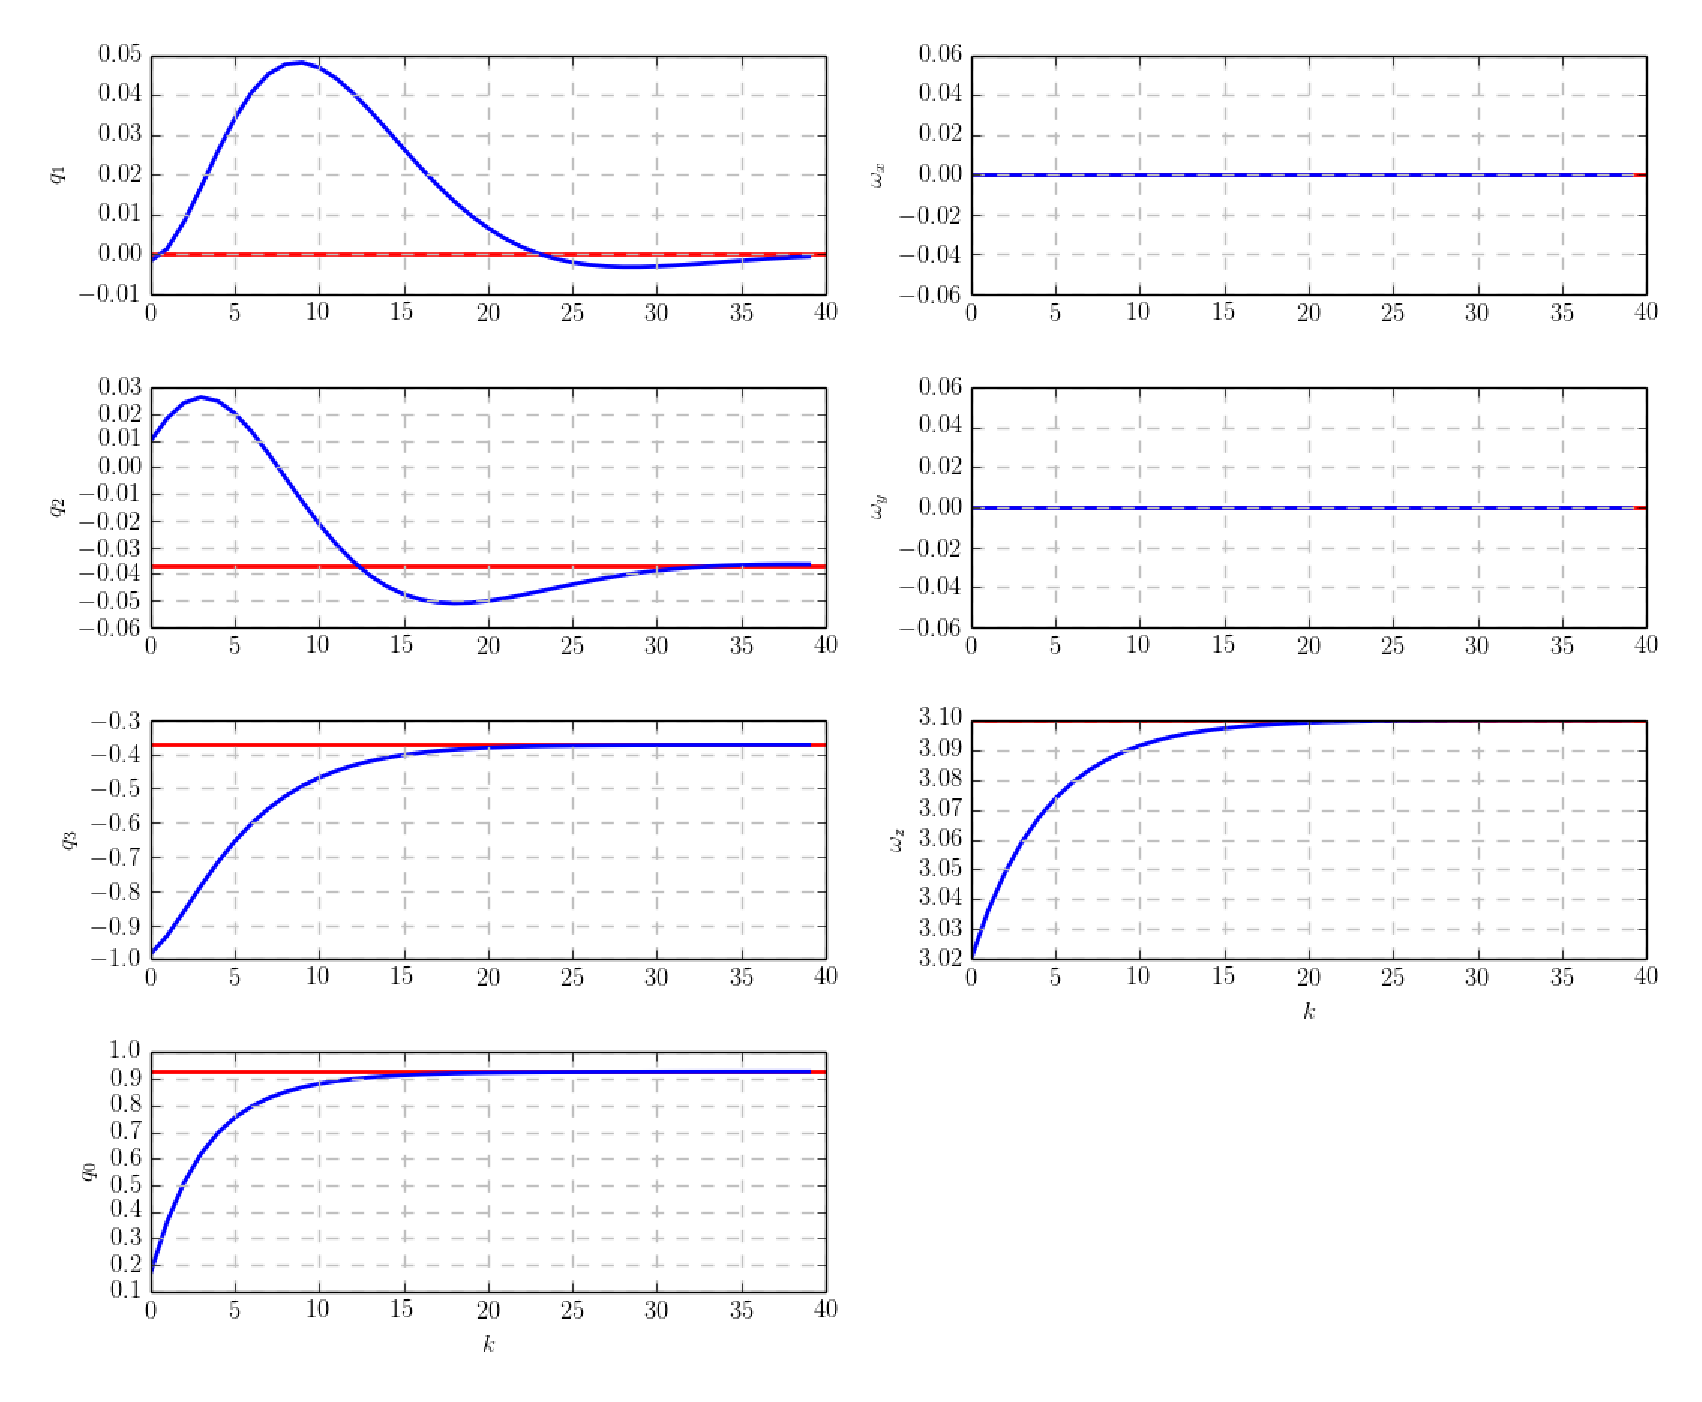
\psfig{file=figures/p_estimator_static_target.eps,width=6in}}
  \caption{P-Estimator with static target}
  \label{fig:PEstimatorwithstatictarget}
\end{figure}

The work covered so far in this chapter has all dealt with the a system in a static state.  In Figure \ref{fig:PEstimatorwithstatictarget}, a P-Estimator converges it's estimated state (blue) to the static measured state (red).  While the estimated state converges to the measured state after about 40 iterations, this type of conversion would be effective only for non-rotating systems.  The non-zero $\omega_z$ means that the quaternion attitude representation will be in constant motion.

The $3.1$ rad/sec rotation about $0\bs{i} + 0.1\bs{j} + 1\bs{k}$ condition from the previous p-estimator is then allowed to propagate the quaternion state through 10 second of rotation with state estimate updates every 0.1 sec.  The resulting measured state (red) and estimated state (blue) is shown in Figure \ref{fig:PEstimatorwithrotatingtarget}.  The body rates track identically to those in Figure \ref{fig:PEstimatorwithstatictarget} where $t(k) = 2$ corresponds to $k = 20$.  Due to the proportional only compensation and no predictive methods, the initial transient behavior is followed by a behavior similar to a steady state error.

\begin{figure}[H]
  \centerline{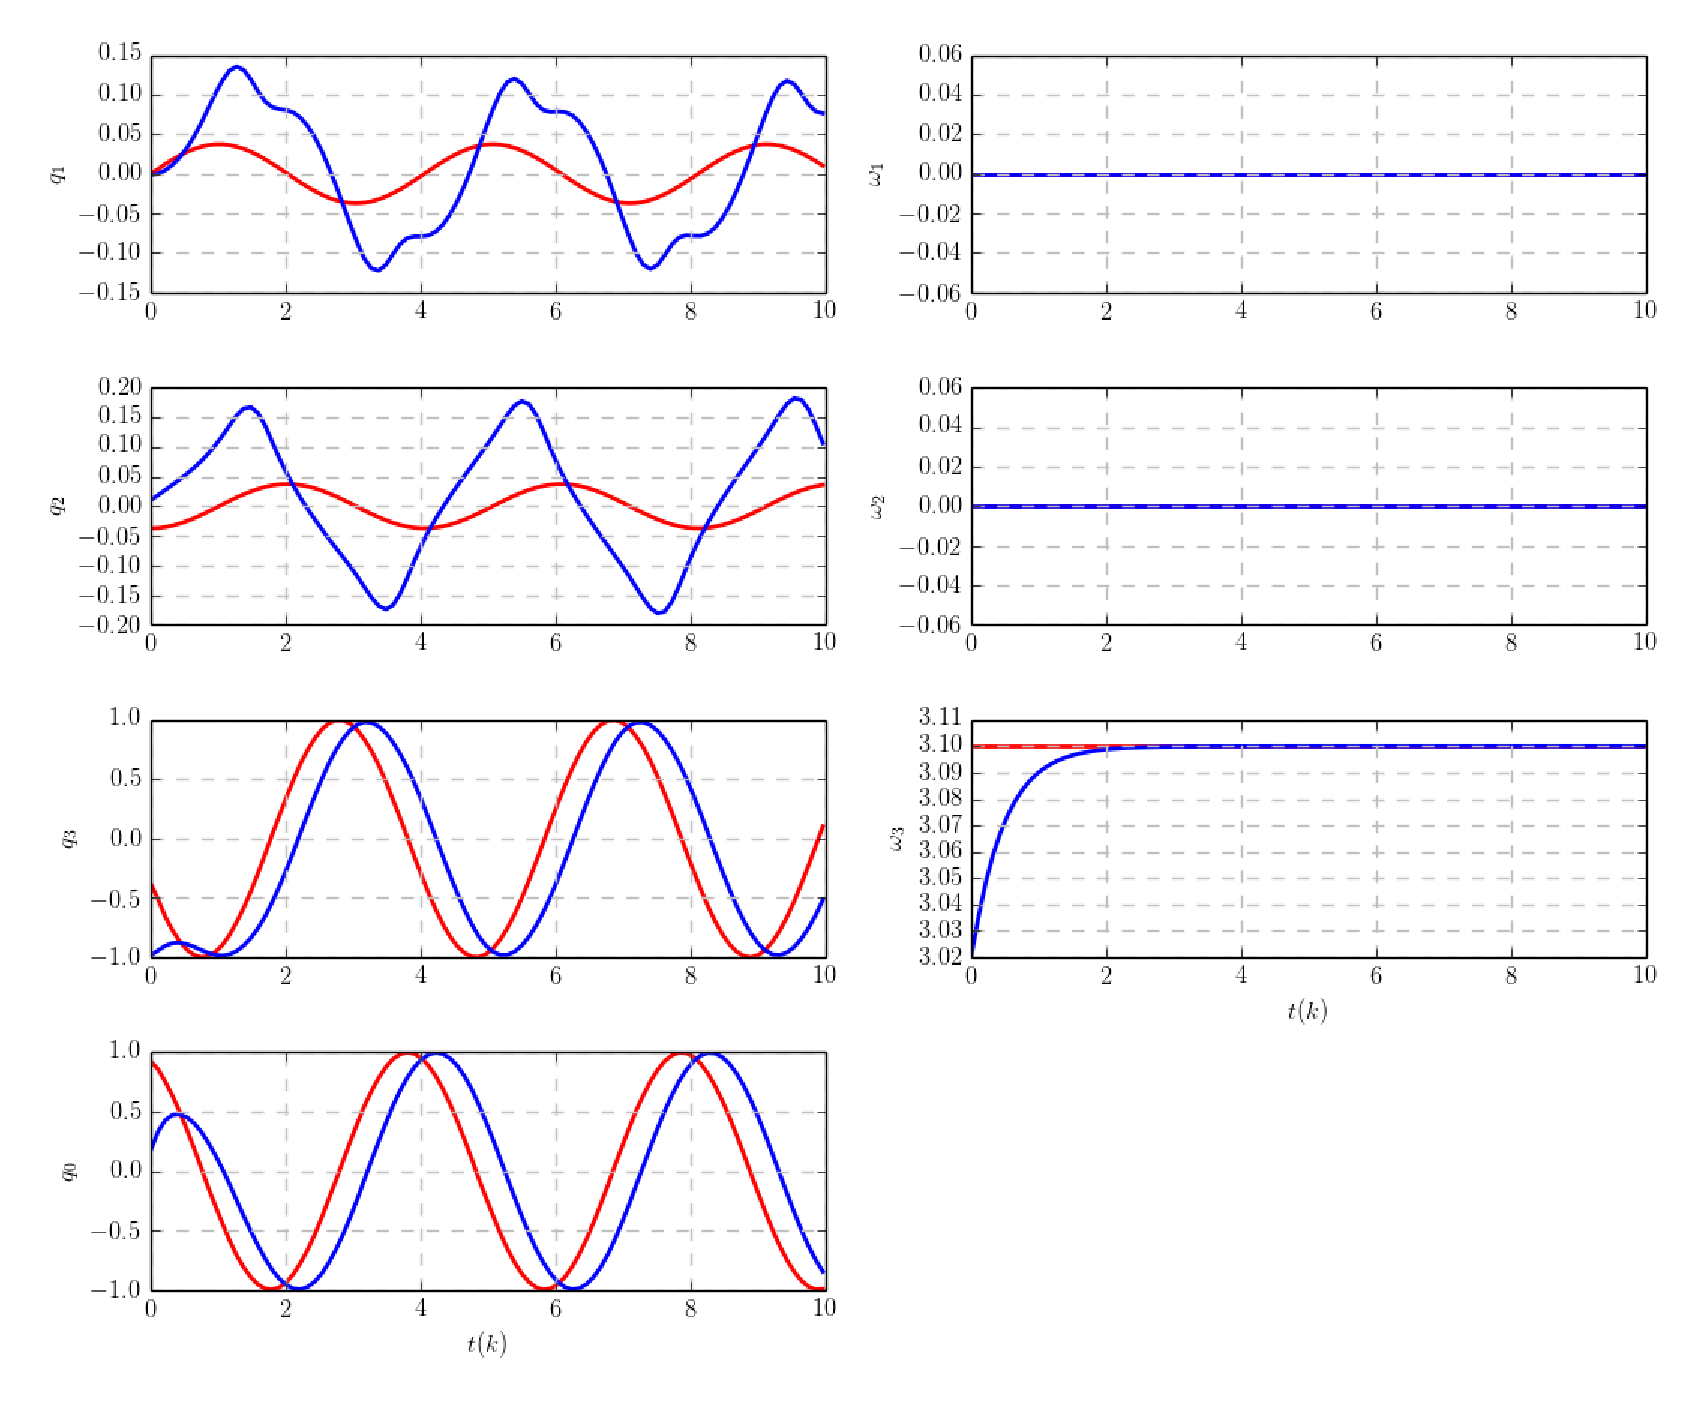
\psfig{file=figures/p_estimator_3radps.eps,width=6in}}
  \caption{P-Estimator with rotating target}
  \label{fig:PEstimatorwithrotatingtarget}
\end{figure}

Increasing the frequency of updates to the p-estimator can decrease the error between the measured and estimated states, but there will always be an error similar to a steady state error in the quaternion representation.  For better results the estimator needs to take into consideration changes in the state through the PID's integration and derivative terms.

\subsubsection{Integral Estimator}
\label{subsubsec:IntegralEstimator}

To stay consistent with the findings in the State Error section (\ref{sec:StateError}), the quaternion portion of the integrated state should abide by the quaternion multiplicative correction method.  This is the first model where the variable sized time step is also taken into consideration.  Instead of accumulating the error measurements, the error corrections should be weighted according to the length of time between updates $t(k+1) - t(k)$.  In a simplified case the integral term should end up the same in the following two update instances.

\begin{table}[H]
  \centering
  \begin{tabular}{r|c|c|c|c|c}
    $t_1 (sec)$ & 0.1 & 0.2 & 0.3 & 0.4 & 0.5 \\ \hline
    $\theta_e$ & 4 & -3 & -3 & -3 & 5 \\
    \\
    $t_2 (sec)$ & 0.1 & & & 0.4 & 0.5 \\ \hline
    $\theta_e$ & 4 &  &  & -3 & 5 \\
  \end{tabular}
  \label{tbl:VariableUpdates}
\end{table}

In $t_1$, regular updates occur every 0.1 sec ending in an integral error value of 0.  In $t_2$, without taking into consideration the variable step sizes would end in an error value of $+6$, but really the -3 error update should be worth three times as much.

Running the state estimator without compensating for variations in time step sizes can create inconsistencies between different experimental runs.  In Figure \ref{fig:IEstimatorwithouttimevariationcompensation}, the integral estimator was updated with a fixed state for 30 seconds.  The estimator was initialized at $0$ radians and run three times against a fixed angle of $0.5$ radians.  The first time with an estimation update frequency of every 0.4 seconds (blue), second with the update frequency of every 0.1 seconds (red), and third with a variable update frequency (green) that jumped back and forth between updating every 0.05 and 0.4 seconds.

\begin{figure}[H]
  \centerline{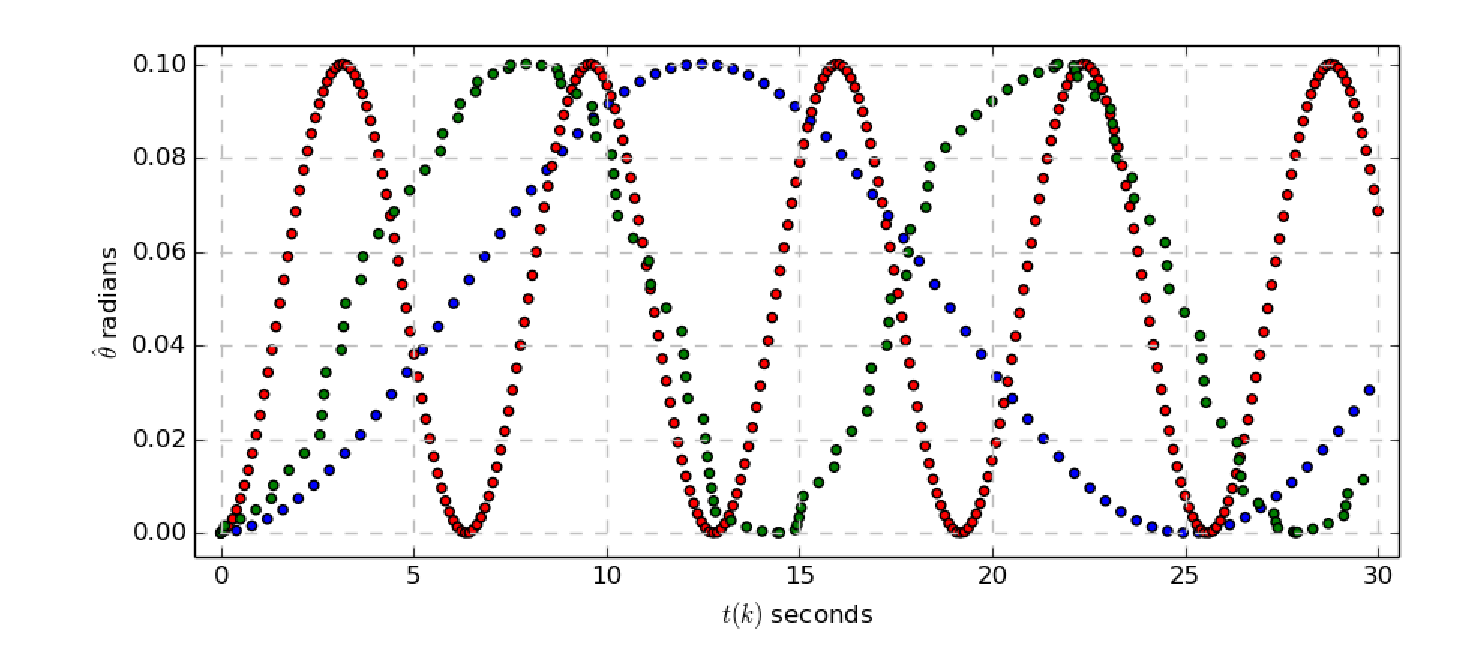
\psfig{file=figures/i_estimator_no_time_varying.eps,width=6in}}
  \caption{I-Estimator without time variation compensation}
  \label{fig:IEstimatorwithouttimevariationcompensation}
\end{figure}

Each calculated estimate for $\hat{\theta}$ in the $k$ domain is identical for each of the three runs, but varies greatly in the time domain.  Most notably, the third run that alternates between update frequencies ends up creating an estimation dynamic that could make the controller less robust.

In comparison, the PID estimator was modified to incorporate the time step size into it's integral term.  The same three tests were run as above with the 0.1 (red), 0.4 (blue), and variable 0.05/0.4 (green) time steps.  The adjustment quaternion method from Section \ref{subsec:RepresentativeStateAdjustments} is first used to compensate for measured time step size of $\Delta t_{k}$ creating a consistent error quaternion. then is used as before to scale the error quaternion by the selected gain value.  The results of this work can be seen in Figure \ref{fig:IEstimatorwithtimevariationcompensation} where the three test runs are still not identical, but their dynamics are more similar than before.  More notably, the variable step test (green) shows less variability in the estimate being produced which will reduce the noise being transferred to the control algorithm.

\begin{subequations}
  \begin{align}
    \bs{\hat{x}}(t_{k+1}) &= \begin{bmatrix} \bs{\hat{q}}(t_{k+1}) \\ \bs{\hat{\omega}}(t_{k+1}) \end{bmatrix} \\
    \bs{\hat{q}}(t_{k+1}) &= \bs{\psi}\big(\bs{q}_{ei}(t_k), K_{qi}\big) \otimes \bs{\hat{q}}(t_{k}) \\
    \bs{q}_{ei}(t_k) &= \bs{\psi}(\bs{q}_e(t_{k}), \Delta t_{k}) \otimes \bs{q}_{ei}(t_{k-1})\\
    \bs{\hat{\omega}}(t_{k+1}) &= \bs{\hat{\omega}}(t_{k}) + \bs{K}_{\omega i} \cdot (\Delta t_k \bs{I})\cdot \bs{\omega}_e(t_{k})
  \end{align}
  \label{eqn:IEstimator}
\end{subequations}

In Equation \ref{eqn:IEstimator}, the error quaternion $\bs{q}_{ei}(t_k)$ used is an accumulation of the time step scaled errors encountered in all previous steps.  This is analogous to a running summation of the error values.  For the body rate estimation, it's largely the traditional integral component with an extra $\Delta t_k \bs{I}$ term that linearly scales the body rate error calculations based on the size of the current time step.

\begin{figure}[H]
  \centerline{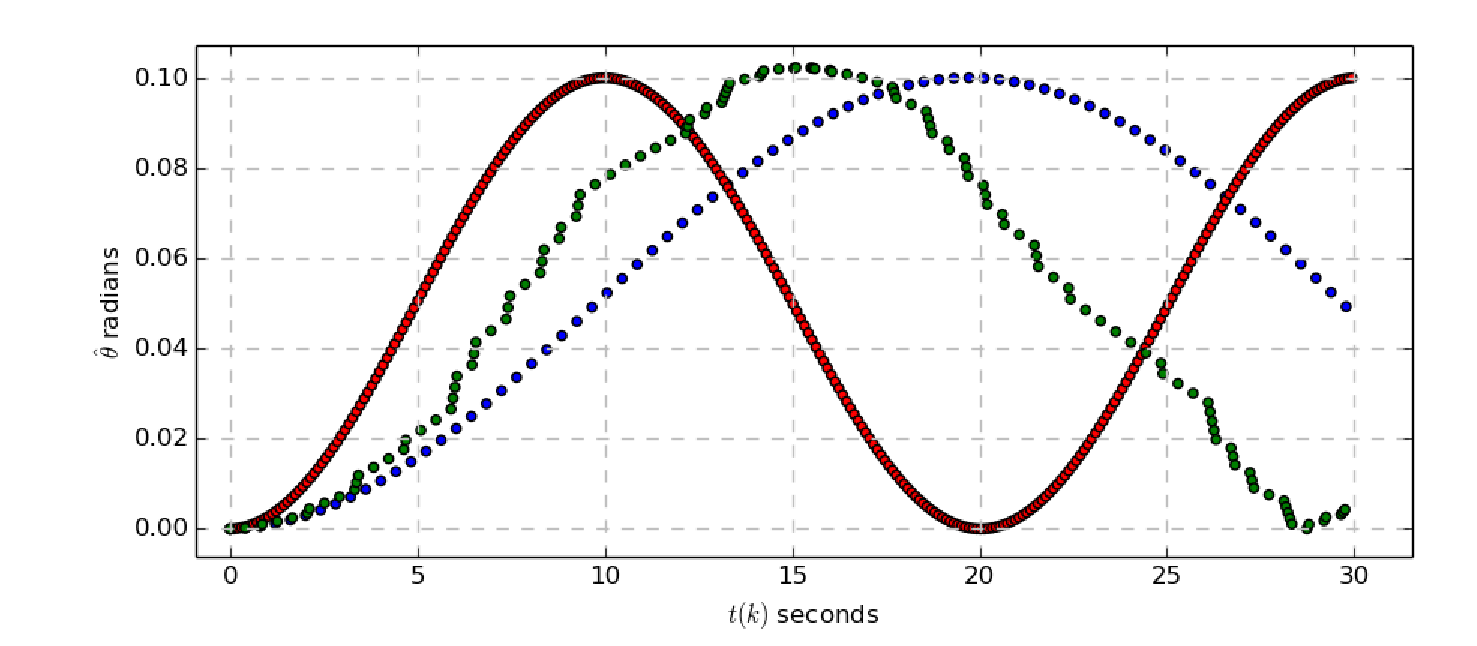
\psfig{file=figures/i_estimator_time_varying.eps,width=6in}}
  \caption{I-Estimator with time variation compensation}
  \label{fig:IEstimatorwithtimevariationcompensation}
\end{figure}

\subsubsection{Derivative Estimator}
\label{subsubsec:DerivativeEstimator}

The derivative component of the PID estimator takes a similar form to the integral component in Equation \ref{eqn:IEstimator}.  The derivative component is only concerned with the current error, previous error, and the current time step size.  As with the integral body rate correction, the derivative correction is scaled by $\frac{1}{\Delta t_k}$ to compensate for variable step sizes.

\begin{subequations}
  \begin{align}
    \bs{\hat{x}}(t_{k+1}) &= \begin{bmatrix} \bs{\hat{q}}(t_{k+1}) \\ \bs{\hat{\omega}}(t_{k+1}) \end{bmatrix} \\
    \bs{\hat{q}}(t_{k+1}) &= \bs{\psi}\left(\bs{q}_{ed}(t_k), K_{qd}\right) \otimes \bs{\hat{q}}(t_{k}) \\
    \bs{q}_{ed}(t_k) &= \bs{\psi}\left(\bs{q}_e(t_{k-1})^* \otimes \bs{q}_e(t_{k}), \frac{1}{\Delta t_{k}}\right)\\
    \bs{\hat{\omega}}(t_{k+1}) &= \bs{\hat{\omega}}(t_{k}) + \bs{K}_{\omega d} \cdot \left(\frac{1}{\Delta t_k} \bs{I}\right) \cdot \bs{\omega}_e(t_{k})
  \end{align}
  \label{eqn:DEstimator}
\end{subequations}

The Figures \ref{fig:DEstimatorwithouttimevariationcompensation} and \ref{fig:DEstimatorwithtimevariationcompensation} below are the results of three test runs with the same set up update frequencies as with the integral component (0.1/sec, 0.4/sec, and varied).  For this comparison, the TableSat was simulated into a steady $0.01$ rad/s rotation about the body $+z$-axis to generate a constant rate of change for the quaternion instead of the fixed quaternion in the integral test.  The $\theta_{adj}$ parameter tracked for this test is the angular rotation associated with the $\bs{\psi}\left(\bs{q}_{ed}(t_k), K_{qd}\right)$ quaternion adjustment term.

\begin{figure}[H]
  \centerline{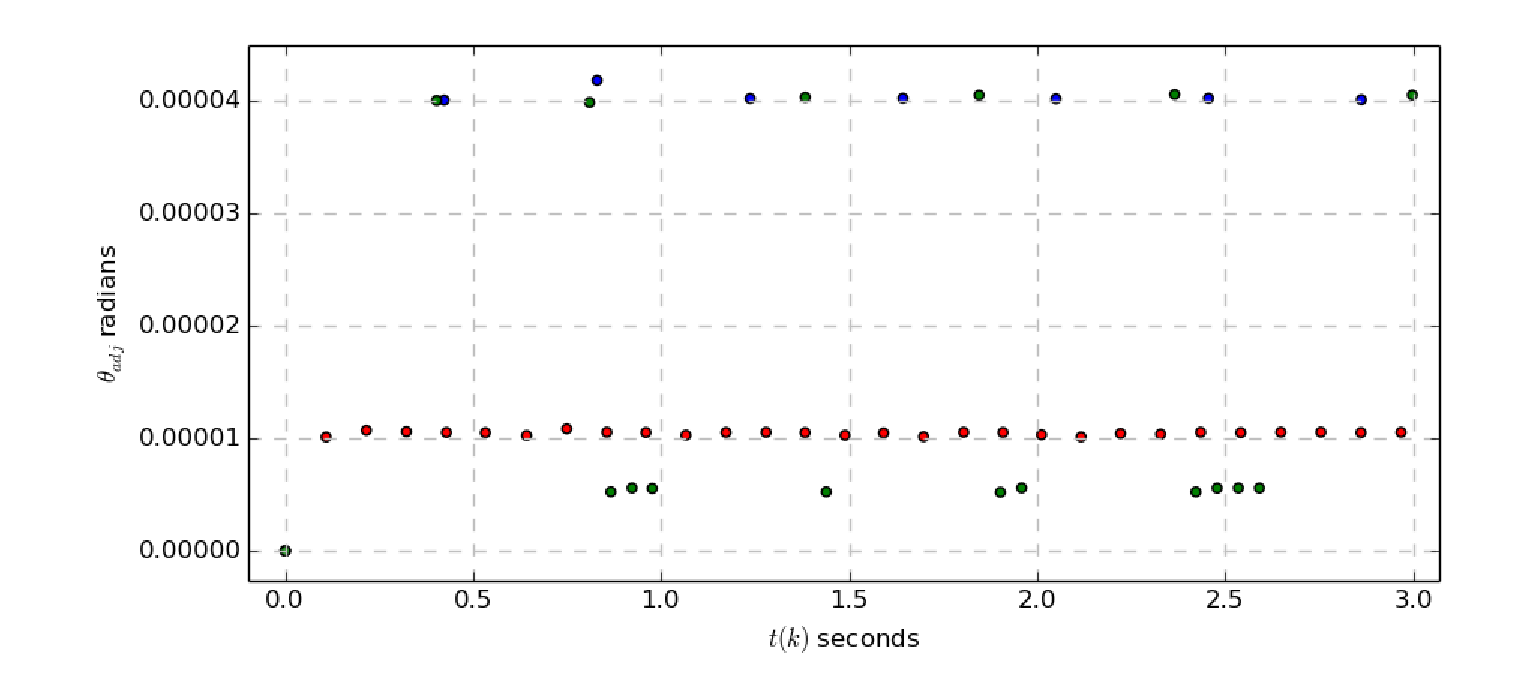
\psfig{file=figures/d_estimator_no_time_varying.eps,width=6in}}
  \caption{D-Estimator without time variation compensation}
  \label{fig:DEstimatorwithouttimevariationcompensation}
\end{figure}

Figure \ref{fig:DEstimatorwithouttimevariationcompensation} shows the results of the test run without consideration taken for time step sizes.  With a constant spin rate, the resulting quaternion adjustment is tightly coupled to the frequency that the updates are made with the 0.1 (red), 0.4 (blue), and variable 0.05/0.4 (green) time steps.  The variable time step sequence is a particular concerns as it jumps back and forth between adjusted amount suggesting the spin rate is not constant.

\begin{figure}[H]
  \centerline{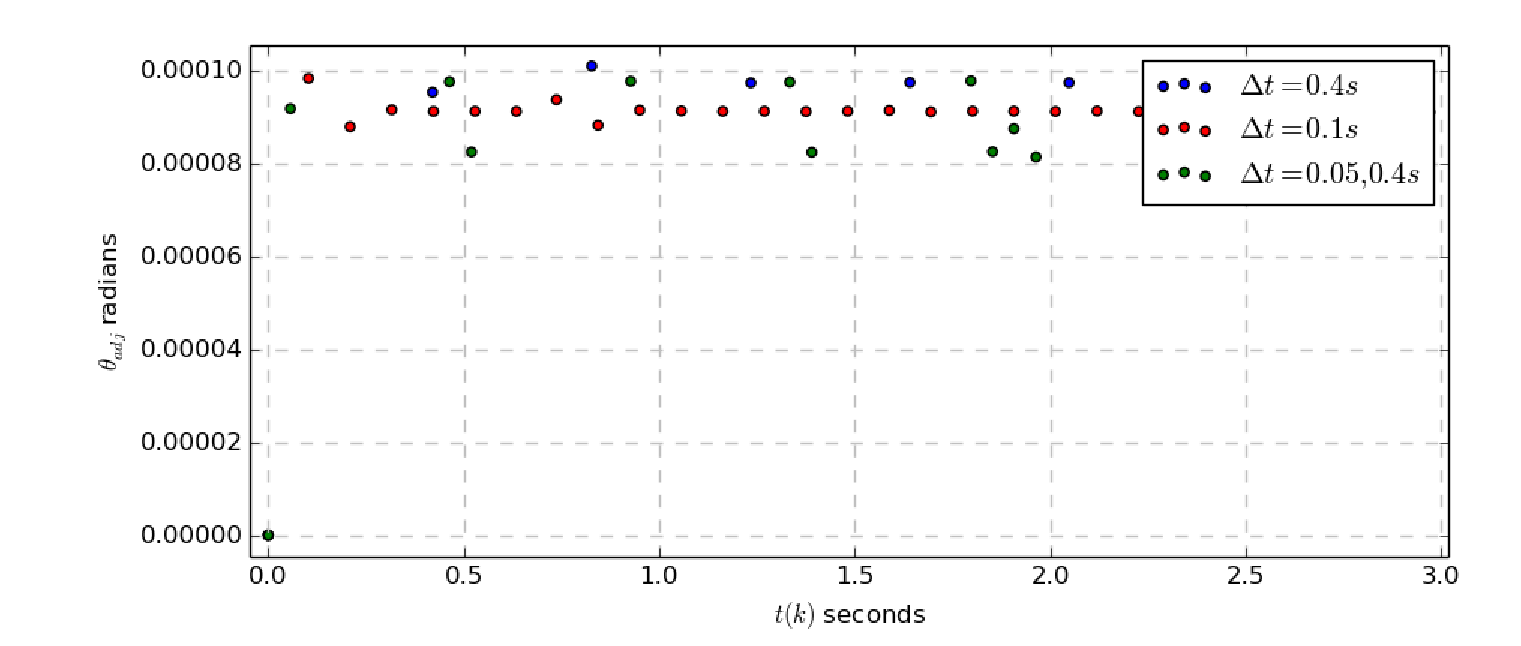
\psfig{file=figures/d_estimator_time_varying.eps,width=6in}}
  \caption{D-Estimator with time variation compensation}
  \label{fig:DEstimatorwithtimevariationcompensation}
\end{figure}

Figure \ref{fig:DEstimatorwithtimevariationcompensation} implements the time variation compensation in Equation \ref{eqn:DEstimator} where the quaternion adjustments provide a better representation of the measured constant spin rate.

\subsubsection{PID Estimation of Unforced Motion}
\label{subsubsec:PIDEstimatorofUnforcedMotion}

Combining the proportional, integral, and derivative estimator portions from above.  Equations \ref{eqn:PEstimator}, \ref{eqn:IEstimator}, and \ref{eqn:DEstimator} get combined into a single PID estimator as

\begin{subequations}
  \begin{align}
    \bs{\hat{x}}(t_{k+1}) &= \begin{bmatrix} \bs{\hat{q}}(t_{k+1}) \\ \bs{\hat{\omega}}(t_{k+1}) \end{bmatrix} \\
    \bs{\hat{q}}(t_{k+1}) &= \bs{\psi}\left(\bs{q}_{ed}(t_k), K_{qd}\right) \otimes \bs{\psi}\big(\bs{q}_{ei}(t_k), K_{qi}\big) \otimes \bs{\psi}(\bs{q}_e(t_{k}), K_{qp})  \otimes \bs{\hat{q}}(t_{k}) \\
    \bs{\hat{\omega}}(t_{k+1}) &= \bs{\hat{\omega}}(t_{k}) + \bs{K}_{\omega p} \cdot \bs{\omega}_e(t_{k}) + \bs{K}_{\omega i} \cdot (\Delta t_k \bs{I})\cdot \bs{\omega}_e(t_{k}) + \bs{K}_{\omega d} \cdot \left(\frac{1}{\Delta t_k} \bs{I}\right) \cdot \bs{\omega}_e(t_{k})
  \end{align}
  \label{eqn:PIDEstimatorUnforcedMotion}
\end{subequations}

The update to the estimated body rate follows the traditional method of the PID control with the addition of the scaling factors for the integral and derivative terms that compensate for non-uniform step sizes at run-time.  The quaternion correction is a compilation of the individual correction quaternions and joined through the multiplicative error correction method.

With a spin stabilized system controlling the body rate is relatively straight forward with a PID controller.  A test was run through TSatPy with based on the PID estimation in Equation \ref{eqn:PIDEstimatorUnforcedMotion}.  The system was set at a spin rate of $0.314$ rad/sec rotation about $+z$ with the measurement of the quaternion angle $\theta$ containing noise $N \sim (0, 0.1218)$ radians.  A gradient descent gain selection settled on the following parameters.

\begin{equation}
  \begin{aligned}
    K_{qp} &= 0.98, K_{qi} = 0.001, K_{qd} = 0.001 \\
    \bs{K}_{\omega p} &= 0.7 \bs{I}, \bs{K}_{\omega i} = \bs{0}, \bs{K}_{\omega d} = \bs{0}
  \end{aligned}
\end{equation}

The test run results are show in Figure \ref{fig:PIDEstimatorwithoutstateprediction}.  The bottom two graphs showing body rate tracking performance where the basic proportional control quickly brings the body rate error under control.  The quaternion estimations are much more difficult largely due to the lack of a system model to convert body rates to estimated attitudes at the next update.  Since the system is spin stabilized and the estimated quaternion has no prior knowledge of where the next value will be, it relies on a large proportional component to jump to the new measurement values on each update.

While testing the performance of the integral and derivative components showed an improved performance when incorporating the effects of the variable time step, in this test with such a heavy reliance on the proportional component, the benefits to considering the variable time step effects were negligible.

\begin{figure}[H]
  \centerline{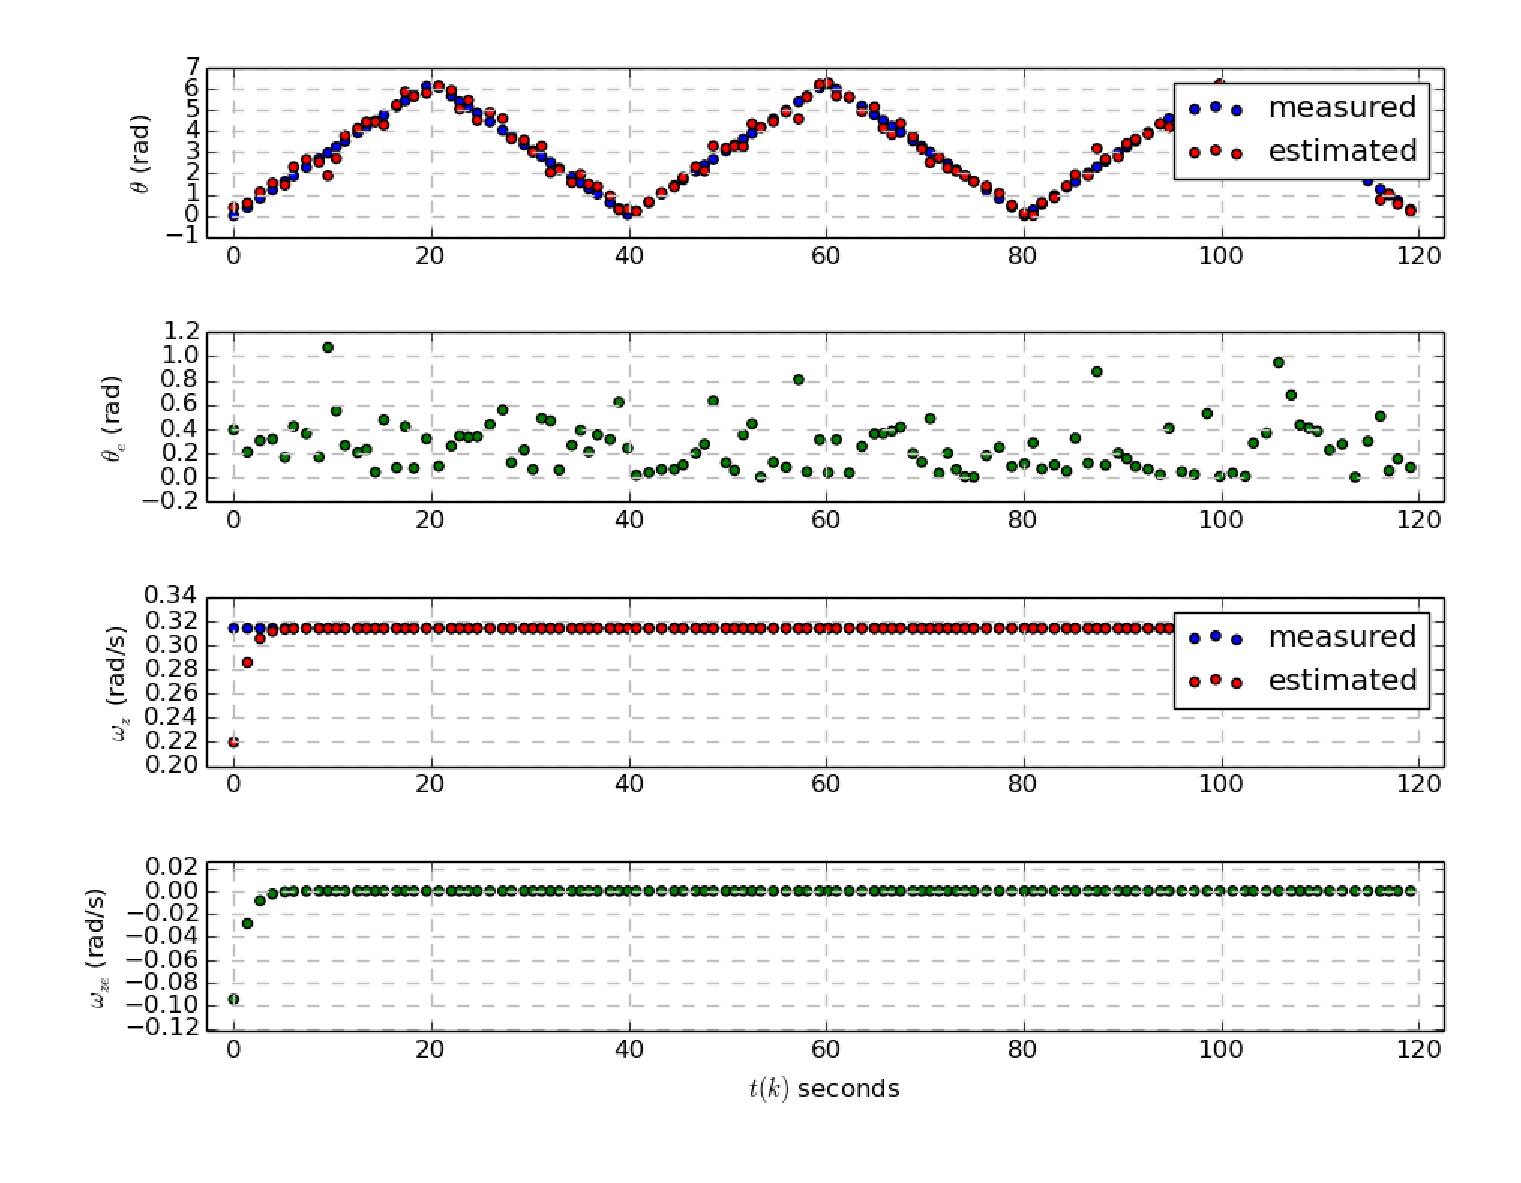
\psfig{file=figures/pid_estimator_no_prediction_high_P.eps,width=6in}}
  \caption{PID-Estimator without state prediction}
  \label{fig:PIDEstimatorwithoutstateprediction}
\end{figure}

\subsection{State Prediction}
\label{subsec:StatePrediction}

Section \ref{subsec:PIDEstimation} shows that to keep accurate tracking of a spin stabilized satellite like TableSat or MMS, the system's dynamic equations are required to couple the body rate and quaternion values.  This is especially important for the TableSat 1A implementation since only the magnetometer and course sun sensors provide feedback about the system's state, and they only have a partial measurement of the attitude quaternion and no direct measurement of the body rates.

The approach taken in the TSatPy code to create state predictions off previous state estimates is to start with a discretized Euler's Moment Equations \ref{eqn:DiscreteEulerMomentEquations} to predict $\bs{\dot{\omega}}(t_{k+1})$.  The the current estimated body rate is adjusted based on the variable time step size.

\begin{equation}
  \bs{\omega}(t_{k+1}) = \bs{\omega}(t_{k}) + \bs{\dot{\omega}}(t_{k+1})\cdot (t_{k+1} - t_k)
\end{equation}

The newly estimated body rates $\bs{\omega}(t_{k+1})$ are supplied to the discretized quaternion dynamics Equation \ref{eqn:DiscreteQuaternionPropagation} to calculate the newly estimated rotational quaternion.

\subsection{PID Estimation with State Prediction}
\label{subsec:PIDEstimatorwithStatePrediction}

From Section \ref{subsec:PIDEstimation}, Equation \ref{eqn:PIDEstimatorUnforcedMotion} defines a method of tracking unforced spin stabilized satellites through PID state estimation.  The biggest issue was a heavy reliance on the proportional gain to track the quaternion attitude which is sensitive to measurement noise.  Incorporating a multiplicative-correction quaternion based model of rigid body dynamics based on the equations in Chapter \ref{chap:SatelliteAttitudeModeling} can assist in predicting the $t_{k+1}$ state of the system.

\begin{subequations}
  \begin{align}
    \bs{\hat{x}}(t_{k+1}) &= \begin{bmatrix} \bs{\hat{q}}(t_{k+1}) \\ \bs{\hat{\omega}}(t_{k+1}) \end{bmatrix} \\
    \bs{\hat{q}}(t_{k+1}) &= \bs{\psi}\left(\bs{q}_{ed}(t_k), K_{qd}\right) \otimes \bs{\psi}\big(\bs{q}_{ei}(t_k), K_{qi}\big) \otimes \bs{\psi}(\bs{q}_e(t_{k}), K_{qp})  \otimes \bs{\hat{q}}(t_{k+1})^- \\
    \bs{\hat{\omega}}(t_{k+1}) &= \bs{\hat{\omega}}(t_{k+1})^- + \bs{K}_{\omega p} \cdot \bs{\omega}_e(t_{k}) + \bs{K}_{\omega i} \cdot (\Delta t_k \bs{I})\cdot \bs{\omega}_e(t_{k}) + \bs{K}_{\omega d} \cdot \left(\frac{1}{\Delta t_k} \bs{I}\right) \cdot \bs{\omega}_e(t_{k})
  \end{align}
  \label{eqn:PIDEstimatorwithPredictionUnforcedMotion}
\end{subequations}

with the a priori state $\bs{\hat{x}}(t_{k+1})^-$ as

\begin{equation}
  \bs{\hat{x}}(t_{k+1})^- = \begin{bmatrix}\bs{\hat{q}}(t_{k+1})^- \\ \bs{\hat{\omega}}(t_{k+1})^- \end{bmatrix} = f \Big( \bs{\hat{q}}(t_{k}), \bs{\hat{\omega}}(t_{k}) \Big)
\end{equation}

The PID estimator now with a state prediction method was run under the same testing conditions present in Figure \ref{fig:PIDEstimatorwithoutstateprediction}.  The resulting performance showed that the inclusion of the system model greatly reduced the reliance on the proportional component of the PID estimator which reduced the noise and increased the accuracy of the final estimates being provided to the controller.  The results in Figure \ref{fig:PIDEstimatorwithstateprediction} show the improved quaternion angle estimates when run with the following gains.

\begin{equation}
  \begin{aligned}
    K_{qp} &= 0.0735, K_{qi} = 0.000863, K_{qd} = 0.00812 \\
    \bs{K}_{\omega p} &= 0.7 \bs{I}, \bs{K}_{\omega i} = \bs{0}, \bs{K}_{\omega d} = \bs{0}
  \end{aligned}
\end{equation}

The quaternion's proportional value is still the dominant gain, but has been reduced by 92.5\% of it's previous value while still providing about 80\% reduction in quaternion attitude error rates.

\begin{figure}[H]
  \centerline{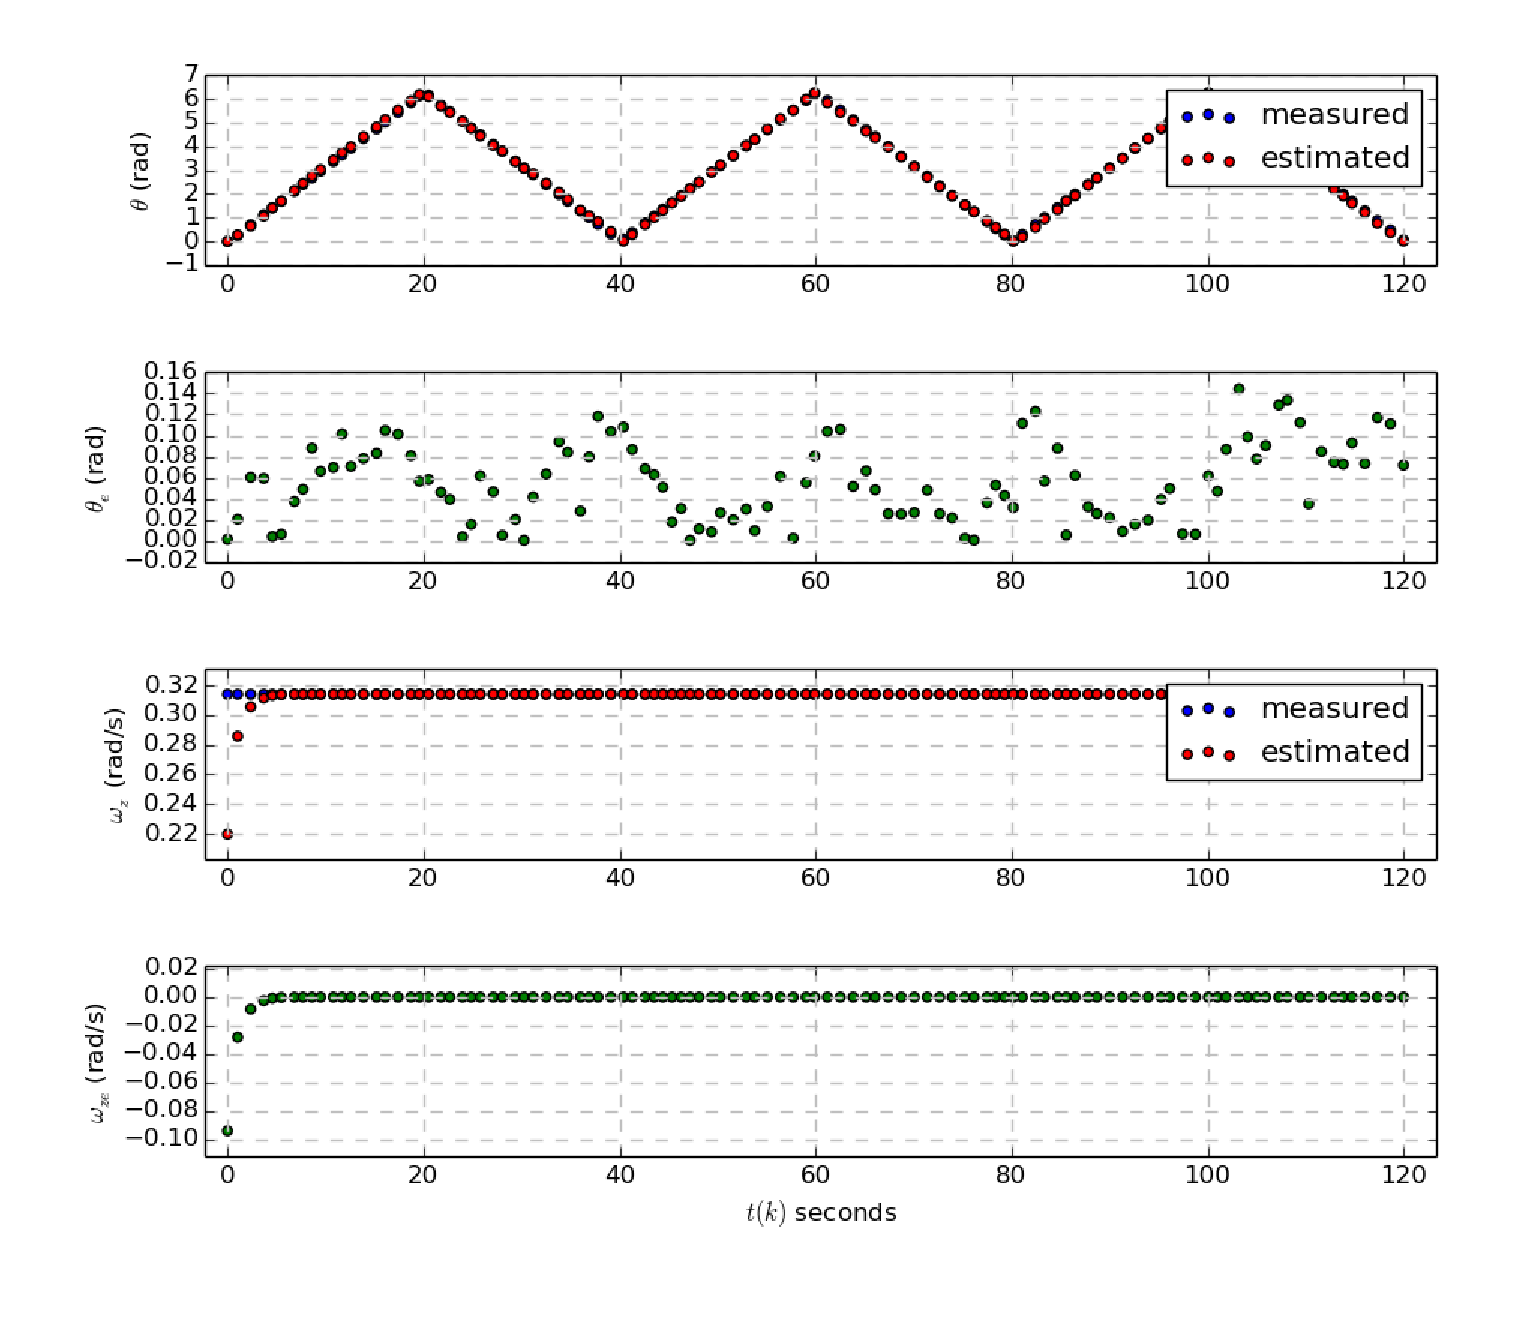
\psfig{file=figures/pid_estimator_with_prediction.eps,width=6in}}
  \caption{PID-Estimator with state prediction}
  \label{fig:PIDEstimatorwithstateprediction}
\end{figure}


\subsection{Sliding Mode Observer}
\label{subsec:SlidingModeObserver}

The Sliding Mode Observer (SMO) is a proportional estimator with an additional smoothing term that uses a chosen sliding surface.  The general form for the SMO is

\begin{equation}
  \bs{\dot{\hat{x}}} = \bs{\hat{f}}(\bs{\hat{x}}, \bs{\hat{u}}, t) + \bs{L}(\bs{C}\bs{\hat{x}} - \bs{C}\bs{x}) + \bs{K}\bs{1}_s\bs{\hat{y}}
  \label{eqn:SMOContinuous}
\end{equation}

Where L is a luenberger gain and $\bs{1}_s$ is a switching function based on $s$.  The sliding mode terms allow additional control of the state adjustments without adding a lot of computational complexity.  The SMO can continue to use the nonlinear model's state predictions as in the PID estimators in Section \ref{subsec:PIDEstimatorwithStatePrediction}, which is an advantage over methods such as the Extended Kalman Filter (EKF) where the system is linearized about an operating point and assumes a constant time step.

This thesis takes the discretized form of Equation \ref{eqn:SMOContinuous} with a quaternion multiplicative correction

\begin{subequations}
  \begin{align}
    \bs{\hat{x}}(t_{k+1}) &= \begin{bmatrix} \bs{\hat{q}}(t_{k+1}) \\ \bs{\hat{\omega}}(t_{k+1}) \end{bmatrix} \\
    \bs{\hat{q}}(t_{k+1}) &= \bs{\psi} (\bs{1}_s\big(\bs{q}_{e}(t_k)\big), K_q) \otimes \bs{\psi}(\bs{q}_e(t_{k}), L_{q})  \otimes \bs{\hat{q}}(t_{k+1})^- \\
    \bs{\hat{\omega}}(t_{k+1}) &= \bs{\hat{\omega}}(t_{k+1})^- + \bs{L}_{\omega} \bs{\omega}_e(t_{k}) + \bs{K}_{\omega}\bs{1}_s \big(\bs{\omega}_e(t_{k}) \big)
  \end{align}
  \label{eqn:SMOEstimatorwithPredictionUnforcedMotion}
\end{subequations}

where

\begin{subequations}
  \begin{align}
    \bs{1}_s\big(\bs{q}_{e}(t_k) \big) &= \begin{bmatrix} \bs{v_e} \\ sat\left( \frac{\cos^{-1} q_{0e} }{S_{q}} \right) \end{bmatrix} \\
    \bs{1}_s \big(\bs{\omega}_e(t_{k}) \big) &= sat\left( \frac{\bs{\omega}_e(t_{k})}{S_{\omega}} \right) \\
    \bs{L}_{\omega} &= L_\omega \cdot \bs{I} \\
    \bs{K}_{\omega} &= K_\omega \cdot \bs{I}
  \end{align}
\end{subequations}

For body rates, the a priori state provides the predicted body rate $\bs{\hat{\omega}}(t_{k+1})^-$ that gets adjusted by a proportional term $\bs{L}_{\omega} \bs{\omega}_e(t_{k})$ as in the P-Estimator, but has an additional saturation function correction based on sliding surfaces for the individual body rate errors.  As found in the PID estimator, the proportional estimator for a steady spin stabilized satellite performs adequately.  The additional saturation term becomes helpful for situations with low $L_\omega$ values that can take longer to converge from the initial body rate to the actual body rate, but once close will increase the effort in staying in step with the measured body rate.

Similar to the PID estimator, the quaternion sliding mode observer limits it's focus to the angular measure of the rotational quaternion.  The sliding surface is taken based on the radian measure.  If the radian measure is below, the saturation limit the quaternion stays as is.  If the quaternion represents a rotation greater than the saturation limit a saturated quaternion is created about the same Euler axis but limit to the saturation angle of rotation.

Running the same tests as run against the PID estimators, the following parameters were located through an iterative gradient descent method that minimized the quaternion error angle and standard deviation of the error angle.

\begin{equation}
  \begin{aligned}
    L_q = 0.362 &, L_w = 0.375 \\
    K_q = 0.308 &, K_w = 0.499 \\
    S_q = 0.419 &, S_w = 0.00517 \\
  \end{aligned}
\end{equation}

Figure \ref{fig:SMOEstimatorwithstateprediction} shows the result of the test at these optimized parameters.  The inverted angle measurement in the first graph is an artifact of the non-unique representation of a quaternion attitude.  In this case, the estimated angles are being calculated for rotations about the body's $-z$-axis instead of the $+z$ axis.  This further supports the decision made in Section \ref{sec:StateError} to use the multiplicative error as the second graph shows the correct error values.

Although the SMO in this case is able to traverse the initial transient response well, the steady state quaternion error is almost as high as using a PID estimator with no state prediction method.  This behavior is due to the high quaternion measurement noise.  With the saturation function, the sliding mode observer is still largely a proportional estimator without the assistance of an integral term to smooth out the noise.

\begin{figure}[H]
  \centerline{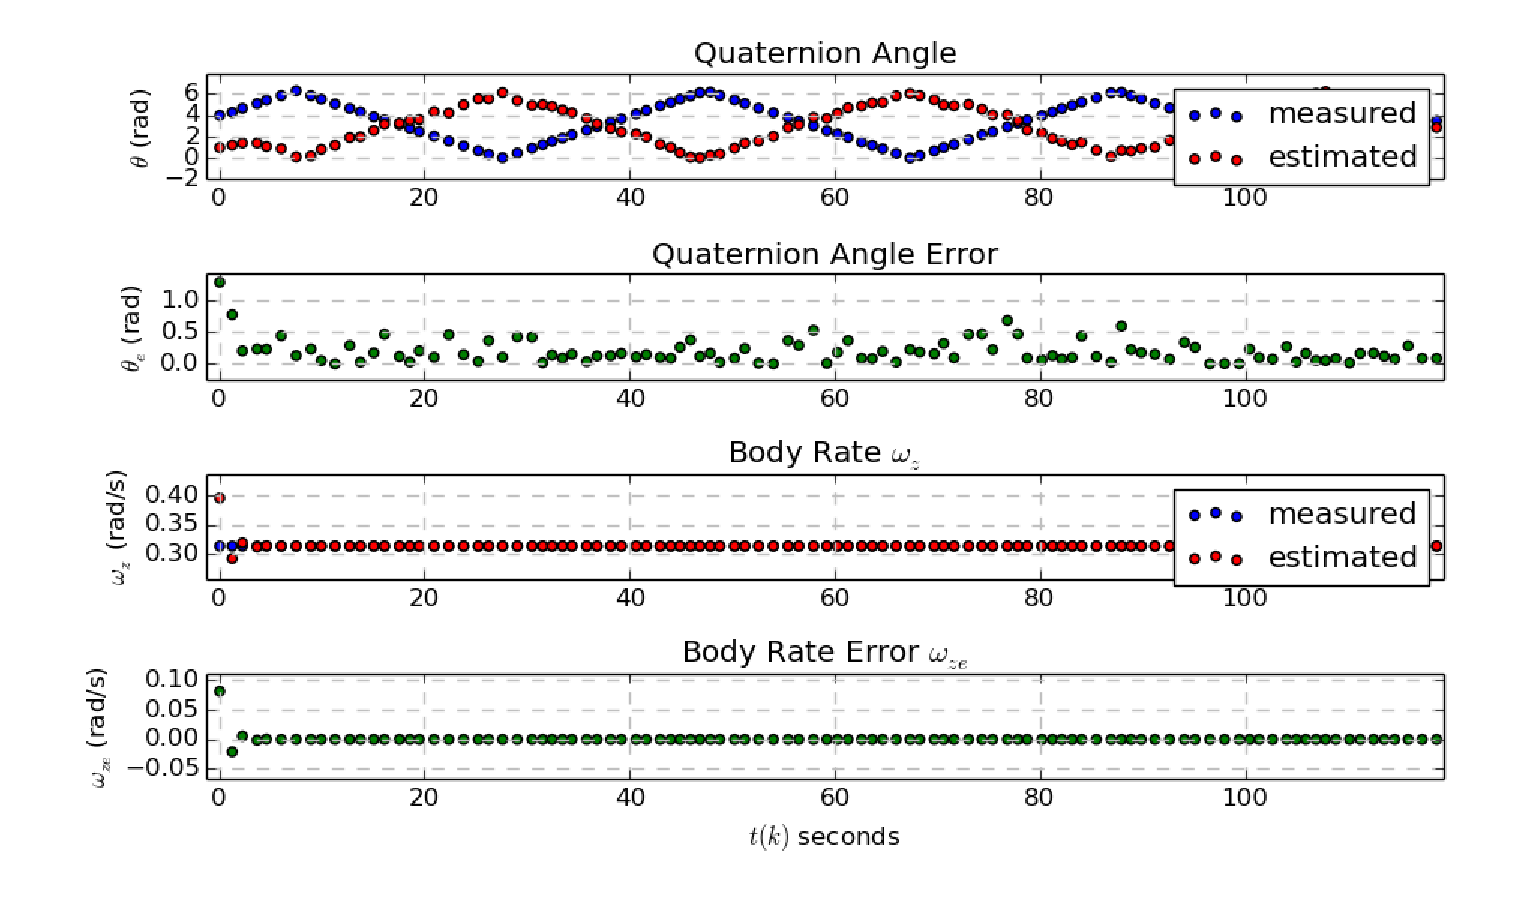
\psfig{file=figures/smo_estimator_with_prediction.eps,width=6in}}
  \caption{SMO-Estimator with state prediction}
  \label{fig:SMOEstimatorwithstateprediction}
\end{figure}

Based on these results, the SMO performs acceptably for the body rate estimation, but according to the steady state error rates, it appears that the PID estimation would be a better use for the steady state attitude tracking.  Both estimators have similar performance profiles which makes it more complicated to determine the better choice.  Section \ref{subsec:ComparativeEstimationTests} will go over how TSatPy can assist with running both estimation techniques in parallel for to provide a more accurate representation.

\subsection{Comparative Estimation Tests}
\label{subsec:ComparativeEstimationTests}

One of the advantages to developing the TSatPy code base for the MMS/TableSat spin stabilized is the ability to run a comparative analysis of multiple estimators at the same time.  The estimators run agnostic to the source of the measurements.  In the sample shown below, the state measurements were generated by a model, but could also be switched to be pulled off the TableSat.

Figure \ref{fig:PIDSMOEstimatorConcurrentComparison} was generated by running a single simulation an providing the truth model's measured state to both a PID and SMO estimator tuned to the parameters selected during individual gain tuning tests above.  This allows for a clear side-by-side comparison of their performance.  Multiple runs all have similar characteristics.  In the initial transient response both estimators are able to converge to a steady state after just a couple updates, but the SMO is able to converge slightly faster each time.  For the steady state response the PID estimator consistently maintains a lower average error, although with a slightly higher standard deviation.  As with the initial response, the SMO estimation values generally update slightly just before the PID estimator.

\begin{figure}[H]
  \centerline{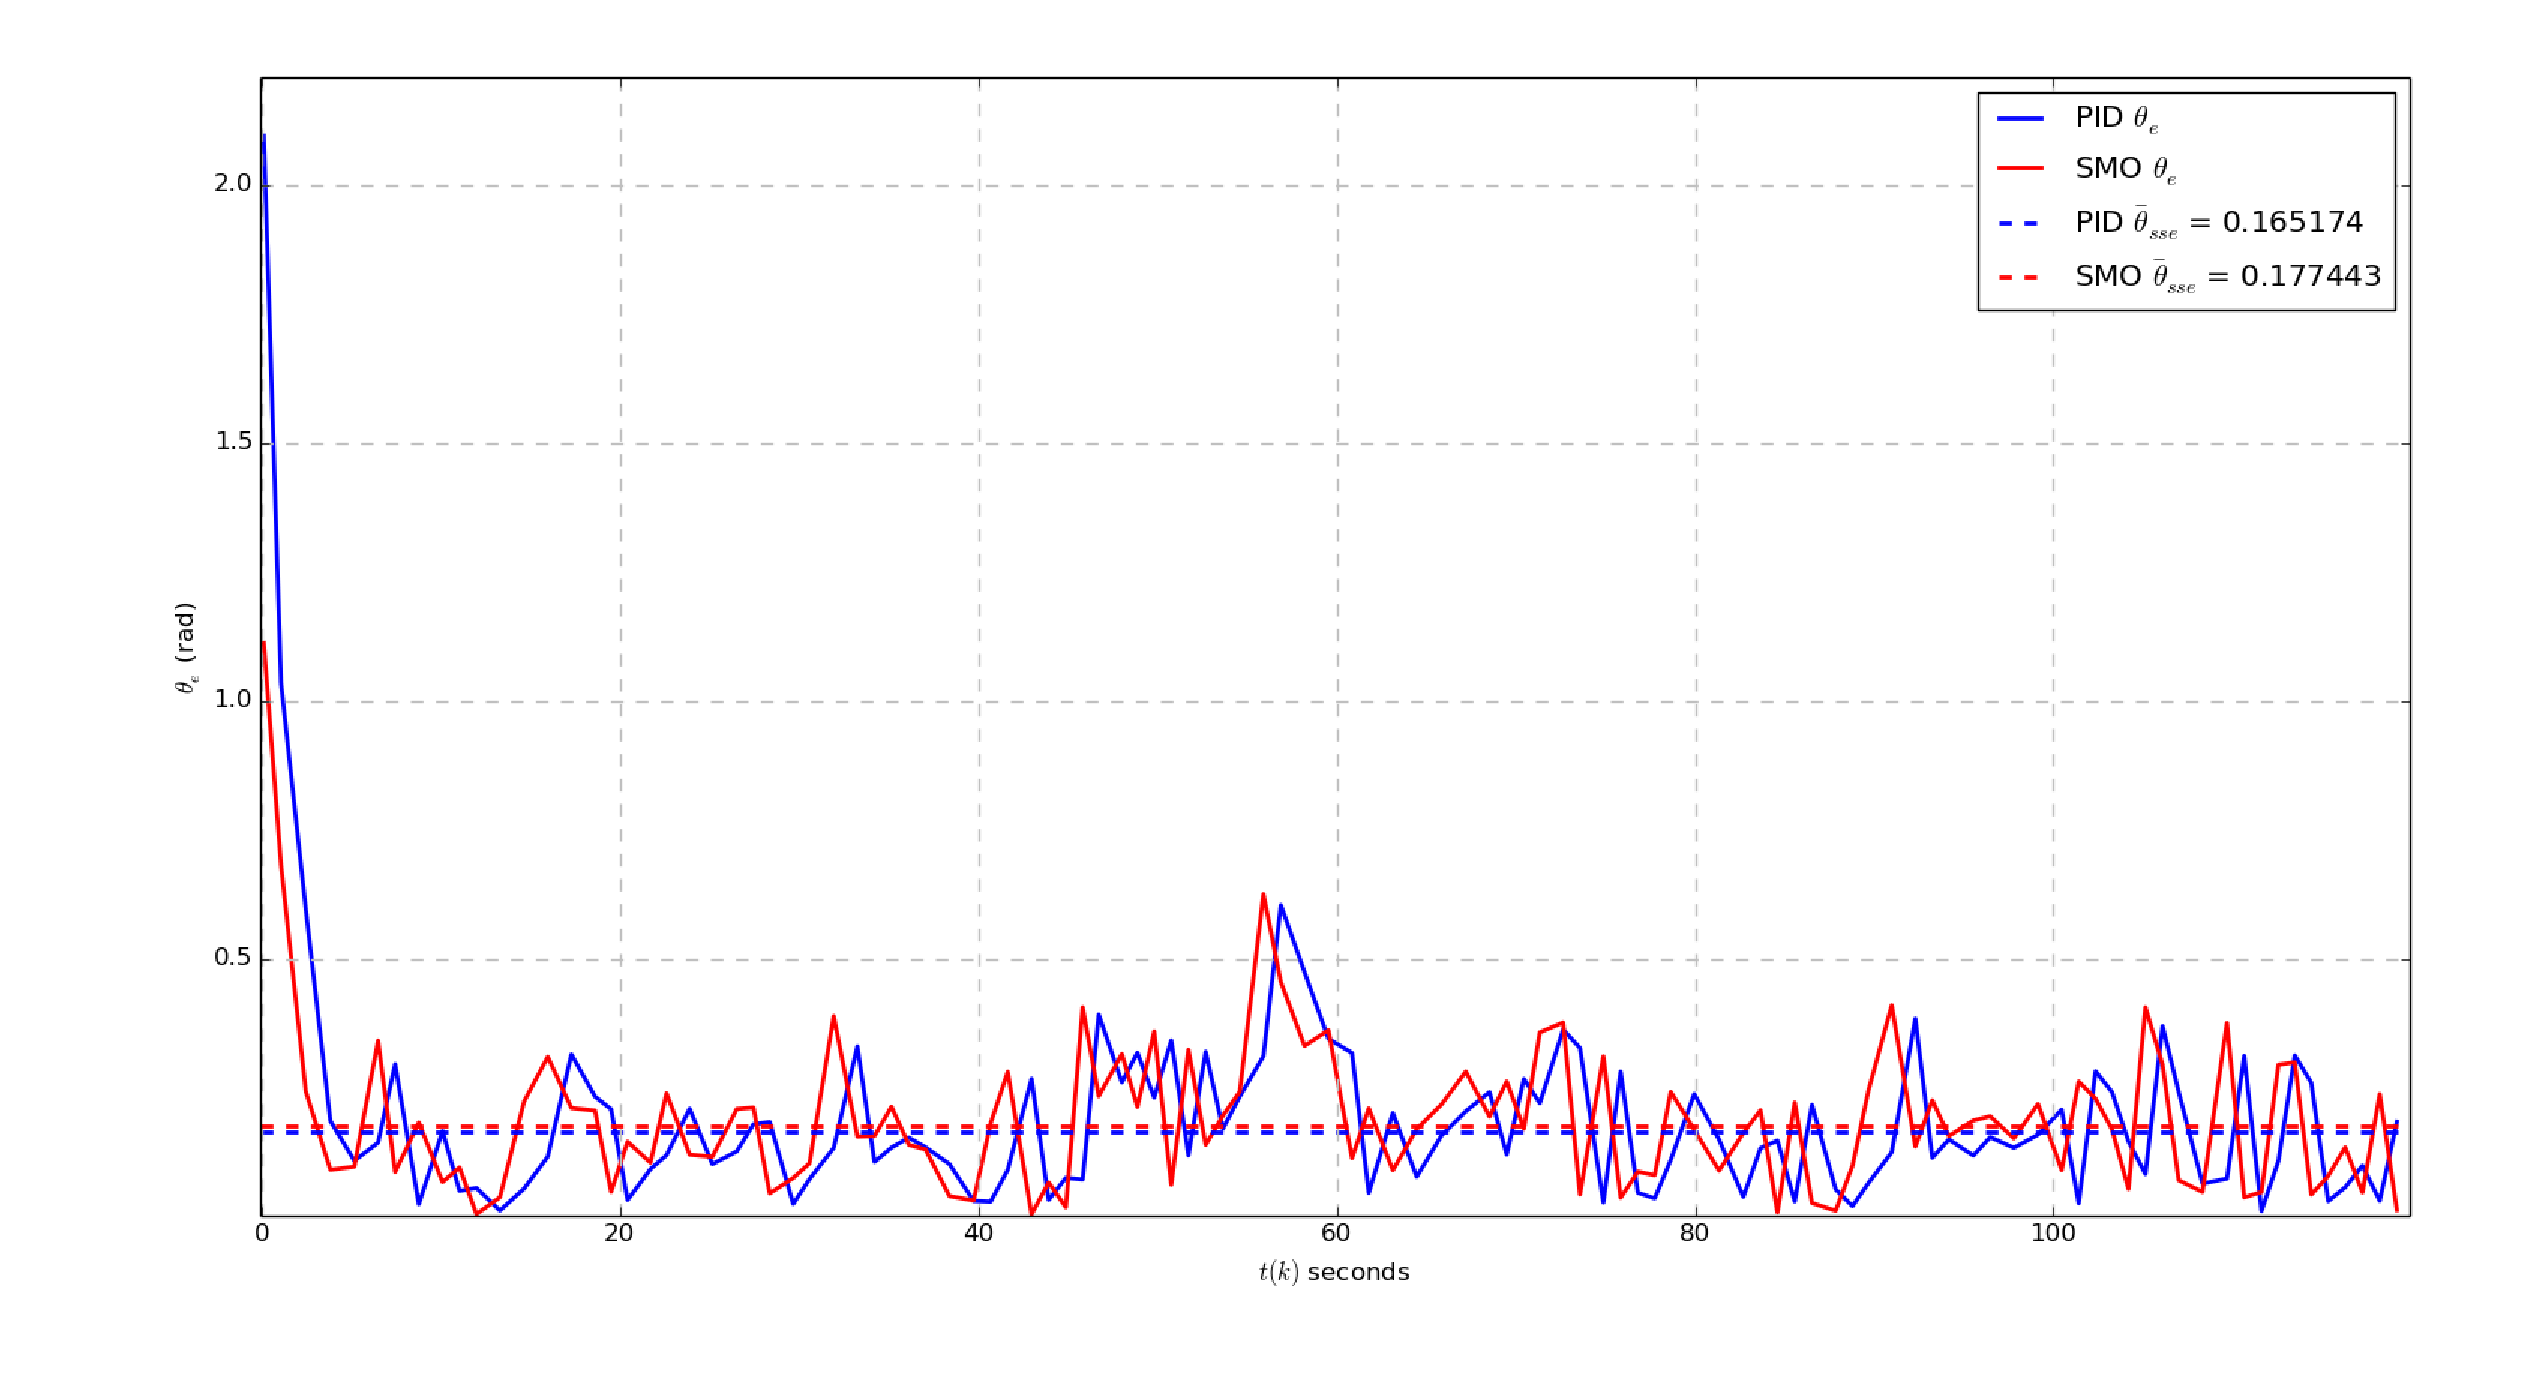
\psfig{file=figures/estimator_comparison.eps,width=6in}}
  \caption{PID/SMO Estimator Concurrent Comparison}
  \label{fig:PIDSMOEstimatorConcurrentComparison}
\end{figure}

The results in Figure \ref{fig:PIDSMOEstimatorConcurrentComparison} were generated through the TSatPy application with the script below.  Lines 10-15 define the two estimators to use in the simulation.  More can be added including the same estimator type with varied parameters.  Lines 17-19 define the system clock behavior.  The simulation will run for a simulated 120 seconds as verified in the results above.  The time steps for each update will vary between 0.8 and 1.2 seconds randomly.  And since this is running as a simulation instead of pulling data from the physical TableSat, the clock can be sped up to run at 10x speed improving the rate of the iterative testing cycle.

\begin{singlespace}
  \begin{minted}[mathescape,linenos,numbersep=10pt,frame=lines,framesep=2mm]{python}
from TSatPy import Estimator, State
from TSatPy.Clock import Metronome
import numpy as np
import matplotlib.pyplot as plt
import time
import random

print('PID / SMO Faceoff')

configs = [{'type': 'pid',
 'args': {'kpq': 0.0735,'kpw': 0.7,'kiq': 0.000863,
          'kiw': 0,'kdq': 0.00812,'kdw': 0}
},{'type': 'smo',
 'args': {'Lq': 0.3619,'Lw': 0.3752,'Kq': 0.3076,
           'Kw': 0.4994,'Sq': 0.4191,'Sw': 0.0052}}]

run_time = 120
speed = 10
dts = [0.8, 1.2]
c = Metronome()
c.set_speed(speed)
I = [[2, 0,  0], [0, 2, 0], [0, 0, 2]]

def setup_estimators(configs):
    x_ic = State.State()
    plant_est = State.Plant(I, x_ic, c)

    est = Estimator.Estimator(c)
    for config in configs:
        est.add(config['type'], plant_est, config['args'])

    return est

def run_comparison(est):
    x_ic = State.State(
        State.Quaternion([0,0,1], radians=4),
        State.BodyRate([0,0,0.314]))
    plant = State.Plant(I, x_ic, c)

    ts = []; smo_err = []; pid_err = []
    start_time = c.tick()
    end_time = c.tick() + run_time
    while c.tick() < end_time:
        plant.propagate()
        offset = np.random.randn() * 20 / 180.0 * np.pi
        q_noise = State.Quaternion([0,0,1], radians=offset) * plant.x.q

        x_m = State.State(q_noise, plant.x.w)

        est.update(x_m)
        ts.append(c.tick() - start_time)

        for model in est.estimators:
            q_e = State.QuaternionError(model.x_hat.q, plant.x.q)
            e, r = q_e.to_rotation()

            if type(model) is Estimator.PID:
                pid_err.append(r)
            elif type(model) is Estimator.SMO:
                smo_err.append(r)
        random.shuffle(dts)
        time.sleep(dts[0] / float(speed))

    return ts, pid_err, smo_err

def graph_it(ts, pid_err, smo_err):
    # Generate the graph here
    # See appendix for the full script

def main():
    est = setup_estimators(configs)
    graph_it(*run_comparison(est))
    return 0

if __name__ == '__main__':
    exit(main())
  \end{minted}
\nocite{minted}
\end{singlespace}

\section{Controllers}
\label{sec:Controller}

The TableSat 1A controller has performance requirements based off of NASA MMS's mission parameters.  Section \ref{subsec:ComparativeEstimationTests} demonstrated that multiple estimators can be run in parallel during both simulations and experimental runs.  As discussed above, this allows for a better insight into performance differences in estimation methods.  An additional benefit to running the controller through TSatPy is the ability to perform estimator scheduling.  Like gain scheduling which for an estimator or controller can modify what gains it uses depending on the current performance, estimator scheduling allows for switching between disparate estimation techniques during run-time.  For example, one estimator tuned for responding to large errors and run along side an estimator tuned for steady state performance.  The control algorithm can then receive more accurate state estimates on a wider range of environmental conditions.

The control requirements for TableSat 1A can be simplified into three main goals.

First is to maintain a steady spin rate of 3 rpm (0.31416 rad/sec).  Given the relative success of the body rate estimation in section \ref{sec:Estimators}, this goal should not be that difficult and likely will not need a complicated control model.

Second is to correct for any nutation out of the spin plane detected by the estimator.  This can take the form of both driving body rates $\omega_y$ and $\omega_z$ to zero, and ensuring the estimated quaternion has an Euler axis is kept in parallel with the global $z$-axis.

Third is to prevent oscillations in the ADP and SDP booms or attenuate any existing oscillations.  Out of the three, this performance goal has the largest set of dependencies for success.  This level of control is reliant on effective actuators along with reliable state estimates based on an accurate system model including boom dynamics.

\subsection{Actuators}
\label{subsec:Actuators}

The actuators in use on TableSat 1A consists of four single directional computer fans.  Two oriented for rate control and two for nutation corrections.  Rate control fans are mounted on opposite sides of the deck in opposing directions.  The two nutation fans are mounted at 90 degree angles and both have their thrust pointing down.  The fans are assumed to be mounted so that the rotation and nutation moments are applied about orthogonal axes, and that the thrust applied is tangential to the body's center of mass.  This initially simplifies the controller's voltage calculations for each fan which can be revisited if testing shows the effects are not negligible.

\begin{figure}[H]
  \centerline{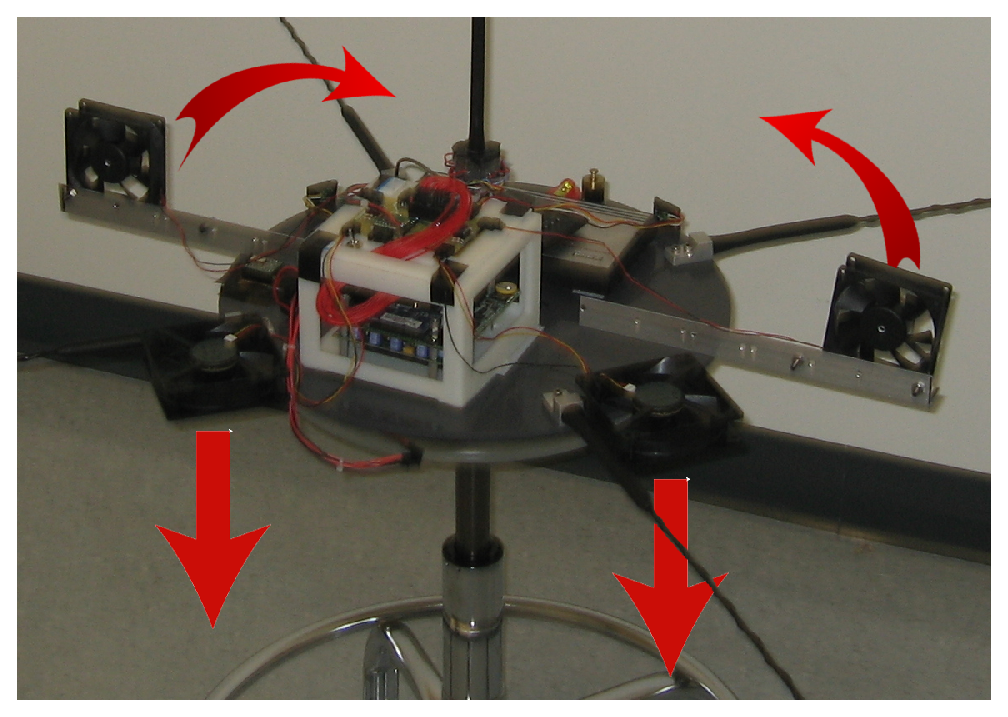
\psfig{file=figures/tsat_thrusters.eps,height=3in}}
  \caption{TableSat 1A thrusters}
  \label{fig:TSatThrusters}
\end{figure}

With this arrangement, actuators are identified by their center, direction of thrust related to the body reference frame, and the maximum force the actuator can produce.

\begin{figure}[H]
  \centerline{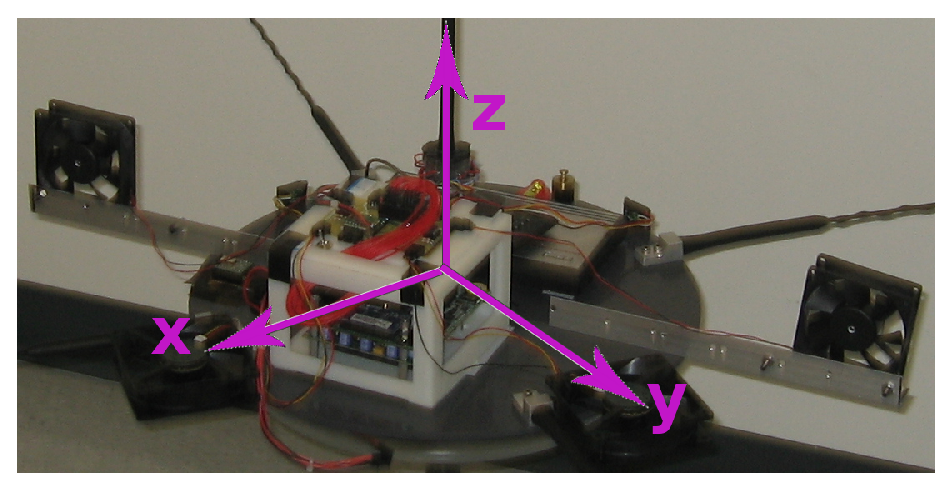
\psfig{file=figures/tsat_body_axes.eps,height=3in}}
  \caption{TableSat Body Axes}
  \label{fig:TableSatBodyAxes}
\end{figure}

\begin{table}[H]
  \centering
  \begin{tabular}{c|c|c|c|c}
    Fan & Center $\bs{f_c}$ (m) & Direction $\bs{n}$ & $F$ (N) & Max Moment $\frac{F \bs{n} \times \bs{f_c}}{|\bs{n}|}$ (Nm) \\ \hline
    1 & $(0.2474, -0.2474, 0)$ & $(-1, -1, 0)$ & 0.08 & $(0, 0, 0.039598)$ \\
    2 & $(-0.2474, 0.2474, 0)$ & $(-1, -1, 0)$ & 0.08 & $(0, 0, -0.039598)$ \\
    3 & $(0.25, 0, 0)$ & $(0, 0, -1)$ & 0.08 & $(0.02, 0, 0)$ \\
    4 & $(0, 0.25, 0)$ & $(0, 0, -1)$ & 0.08 & $(0, -0.02, 0)$ \\
  \end{tabular}
  \caption{Actuator configuration}
  \label{tbl:ActuatorConfiguration}
\end{table}


The role of the actuator module is to accept a desired moment in $\Re^3$ about the body's frame of reference and return what moment is capable with the limited actuator configuration and single direction fans.  The configuration listed in lines 4-13 represent the fan configuration displayed in Figure \ref{fig:TSatThrusters} with the addition of a hypothetical second clockwise fan to demonstrate how the request can be distributed among multiple fans if available.

In the ``setup\_actuators'' function, each fan configuration is fed into the module which calculates the maximum possible moment using the fan's location, direction, and force.

\begin{equation}
  M = \frac{F \bs{n} \times \bs{f_c}}{|\bs{n}|}
\end{equation}

Lines 31-36 list the potential moments for each of the actuators loaded.  Lines 26-28 simulate a request by the controller module for a $(0.03, 0.01, 0.07)$ Nm moment.  Since the fans are mounted to create moments about one of the body reference frame axes, each component of the request is considered separately.  The $M_x = 0.03 Nm$ request can only be partially fulfilled by the Nx fan at max thrust producing a $0.02 Nm$ moment.  The $M_y = 0.01 Nm$ request is within the limits of the Ny fan but because the fan is single directional, the request can not be filled.  The $M_z = 0.07 Nm$ request can not be served by either the CCW1 or CCW2 fans alone but can be generated by both fans if they share the load.  The actuator module splits the request equally between the two CCW fans at 88\% of their max capacity.  In the end, of the initial $(0.03, 0.01, 0.07) Nm$ request is reduced to an attainable moment of $(0.02, 0, 0.07) Nm$.  At this point the information is provided to both``set\_level'' function that would relay the appropriate voltage requirements to the TableSat.  To finish up the request, the actuator module returns the attained moment which can enter a feedback to the estimator and control modules for more accurate system modeling.

\begin{singlespace}
  \begin{minted}[mathescape,linenos,numbersep=10pt,frame=lines,framesep=2mm]{python}
import numpy as np
from TSatPy.Actuator import Actuator

configs = [{'type': 'fan', 'args': {'name': 'CW',
  'center': (0.2474, -0.2474, 0), 'direction': (-1, -1, 0), 'F': 0.08}
},{'type': 'fan', 'args': {'name': 'CCW1',
  'center': (-0.2474, 0.2474, 0), 'direction': (-1, -1, 0), 'F': 0.08}
},{'type': 'fan', 'args': {'name': 'CCW2',
  'center': (-0.2474, -0.2474, 0), 'direction': (1, -1, 0), 'F': 0.08}
},{'type': 'fan', 'args': {'name': 'NY', 'center': (0.25, 0, 0),
  'direction': (0, 0, 1), 'F': 0.08}
},{'type': 'fan', 'args': {'name': 'NX', 'center': (0, 0.25, 0),
  'direction': (0, 0, 1), 'F': 0.08}}]

def set_level(act, power_level):
    print 'Setting power level=%g for: %s' % (power_level, act)

def setup_actuators(configs):
    act = Actuator()
    for config in configs:
        act.add(config['type'], set_level, config['args'])
    return act

act = setup_actuators(configs)
print(act)
M = np.mat([0.03, 0.11, 0.07]).T
print("Request moment: %s" % (M.T))
print("Applied moment: %s" % (act.request_moment(M).T))

# Prints Out
# Actuator
#  <Fan CW moment=(0, -0, -0.0279901)>
#  <Fan CCW1 moment=(0, 0, 0.0279901)>
#  <Fan CCW2 moment=(0, 0, 0.0279901)>
#  <Fan NY moment=(0, -0.02, 0)>
#  <Fan NX moment=(0.02, 0, 0)>
# Request moment: [[ 0.03  0.11  0.07]]
# Setting power level=1 for: <Fan NX moment=(0.02, 0, 0)>
# Setting power level=1 for: <Fan CCW1 moment=(0, 0, 0.0279901)>
# Setting power level=1 for: <Fan CCW2 moment=(0, 0, 0.0279901)>
# Applied moment: [[ 0.02        0.          0.05598023]]
  \end{minted}
\nocite{minted}
\end{singlespace}

Prior implementations of TableSat generally stuck with a static actuator layout which requires a significant portion of time to rewrite code and/or rewire electronics to assess variations on the actuator layout.  With the use of TSatPy, most modifications to the actuators during testing can be done with just a change to the config structure that provides a much faster turn around time between tests.

\subsection{Rate Control}
\label{subsec:RateControl}

The first of the three controls goals introduced at the start of Section \ref{sec:Controller}, is the rate control of the TableSat/MMS to control the $\omega_z$ body rate at a slow and steady $0.314$ rad/s while any body rates about the $\omega_x$ and $\omega_z$ axes be removed.  The rate controller works on the premise of accepting the estimator's guess at the state of the system and comparing that to a desired state.  Correction moments, $\bs{M}$, are calculated based on any differences in the estimated and desired states.

\begin{equation}
  \bs{M}(t_{k+1}) = f(\bs{\hat{x}}(t_{k+1}), \bs{x}_d, t)
  \label{eqn:GeneralRateControl}
\end{equation}

\subsubsection{PID Rate Control}
\label{subsubsec:PIDRateControl}

A PID rate controller works very similar to the PID estimator.  The input to the estimator is two states with one composite state as the output.  The PID controller takes two states as input as well, but creates moments about the principle axes $M_x, M_y, M_z$.

A proportional controller is more than adequate level of control for a system with perfect measurements since the proportional component is not corrupted by noise.  Figure \ref{fig:PRateControl} shows the response to a randomly assigned initial body rates and how they converge to the desired state of $\omega_z = 0.314$ rad/sec and $\omega_x = \omega_y = 0$ rad/sec.

\begin{equation}
  \bs{M}(t_{k+1}) = \bs{K}_{\omega p} \left( \bs{\omega}_d - \bs{\hat{\omega}}(t_{k+1}) \right)
  \label{eqn:GeneralRateControl}
\end{equation}

\begin{figure}[H]
  \centerline{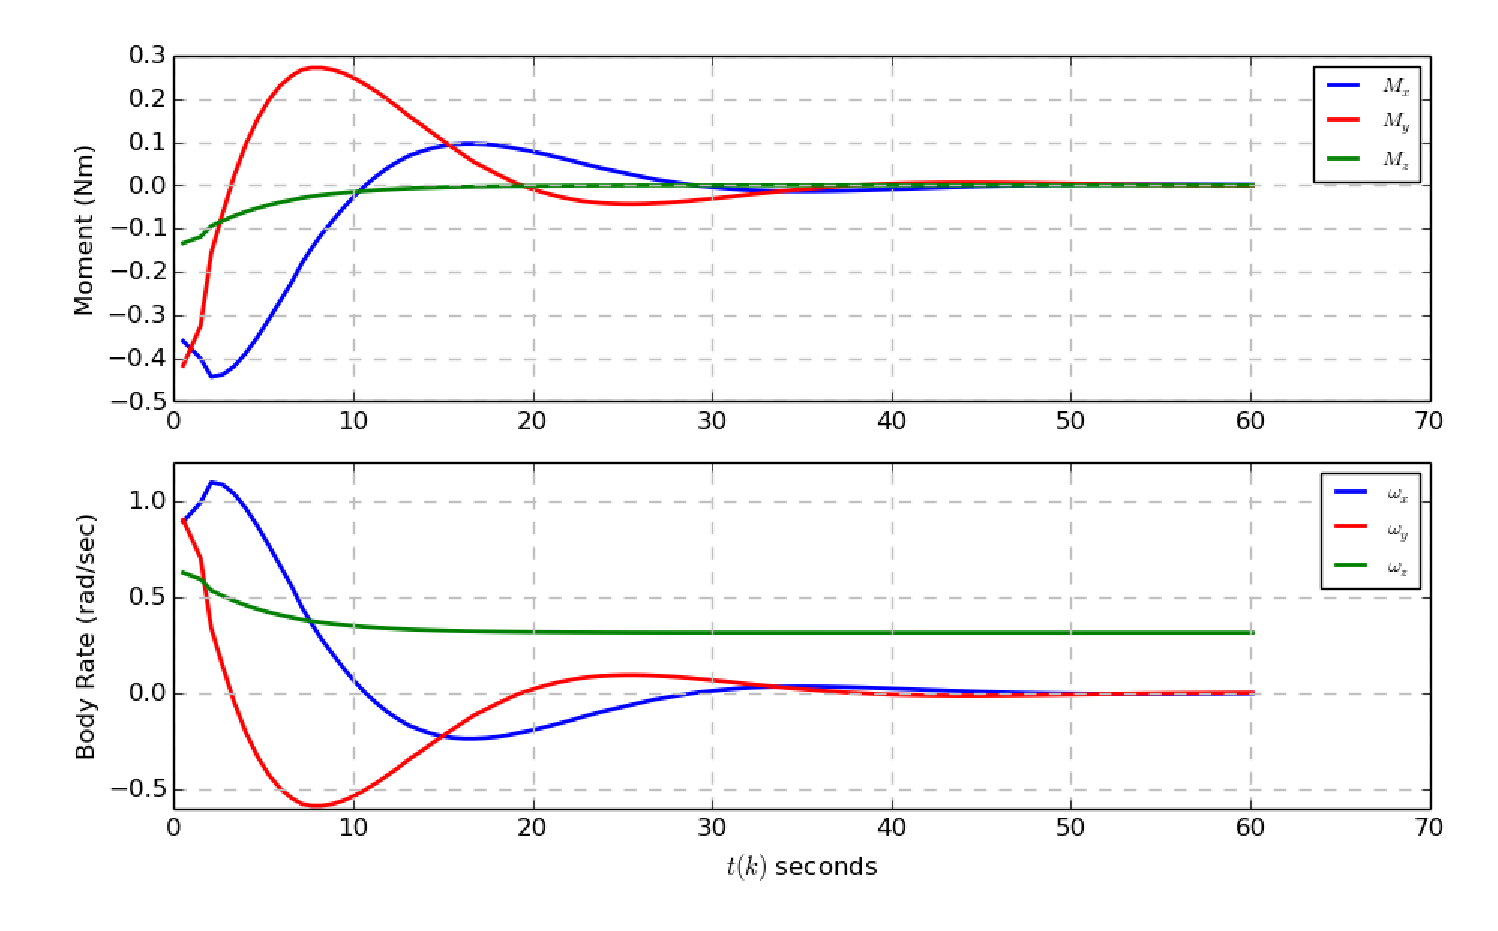
\psfig{file=figures/p_rate_control.eps,width=6in}}
  \caption{P rate control}
  \label{fig:PRateControl}
\end{figure}


\subsubsection{Sliding Mode Controller}
\label{subsubsec:SlidingModeController}



\subsection{Nutation Correction}
\label{subsec:NutationCorrection}

Assuming the system has been brought up to the desired operating conditions, there are a minimum of two checks that are required to determine if the system continues to stay in the desired state.

\begin{equation}
  \begin{aligned}
    \omega_z &= 3 \text{ rpm} \\
    \bs{v} \bullet (0\bs{i}+0\bs{j}+1\bs{k}) &= \left\{ \begin{array}{lr} 1 & : q_0 > 0 \\ -1 & : q_0 < 0 \end{array} \right.
  \end{aligned}
  \label{}
\end{equation}

Correcting for variations in $\omega_z$ follows standard control theory methods.  Correcting for variation in the Euler vector are more complicated especially when keeping with multiplicative correction methods instead of state difference methods as was determined in Section \ref{sec:StateError}.  Keeping the two state requirements decoupled is advantageous if possible.  Even though the rate of the quaternion can be used to help control the body rate, if the control of the quaternion is limited to aligning the vector component with the global $z$-axis, the body rate controller can focus on correcting for any errors in the spin rate.

\subsection{Quaternion Decomposition}
\label{subsec:QuaternionDecomposition}

\subsection{Boom Dynamics}
\label{subsec:Boom Dynamics}








\begin{equation}
  \bs{\omega}_d = \begin{bmatrix} 0 & 0 & 0.31416 \end{bmatrix}^T
  \label{eqn:DesiredBodyRate}
\end{equation}

Since the satellite is spin stabilized, the desired quaternion is not as straight forward.  With a goal of keeping the body's $z$-axis aligned with the global reference frame's $z$-axis the $q_3$ and $q_0$ quaternion values should be allowed to vary as $q_1$ and $q_2$ should remain at zero if no nutation exists.

\begin{equation}
  \bs{q}_d = 0 \bs{i} + 0 \bs{j} + q_3 \bs{k} + q_0
  \label{eqn:DesiredQuaternion}
\end{equation}


\TODO{Finish this}

\section{Simulations}
\label{sec:Simulations}

\TODO{Finish this}

\chapter{Standard Control Theory Tools}
\label{chap:StandardTools}

\section{Simulink}
\label{sec:Simulink}

Slight variation of the ``open loop'' control system used in part of Melissa Vess' TableSat research.  Huge problem with fault tolerance.  The format chosen for relaying messages resulted in an unreliable exchange of data between the base station (laptop) and the TableSat.  These error were compounded with Matlab Simulink's inability to handle the unexpected lack of message data.

\TODO{More detail here on the Simulink side.  Specify pros of this design.  Include screen shot of simulink diagram for a P controller.}


\section{TSat Message Center}
\label{sec:TSatMessageCenter}

This was the first full rework of the control system.  The focus of this design was to eliminate the use of Matlab Simulink diagrams, and directly control the messages transmitted and received.

\TODO{Elaborate on the failures of the design.  Inability to handle two tasks at one.  State persistence.  No visualization.  }



\chapter{SOFTWARE DEVELOPMENT FOR EXPERIMENTAL INTEGRATION}
\label{chap:SoftwareDevelopmentforExperimentalIntegration}

\TODO{Finish this}

\section{Runtime Control and Analysis}
\label{sec:RuntimeControlandAnalysis}

\TODO{Finish this}

\section{Object Oriented NSS Control System}
\label{sec:ObjectOrientedNSSControlSystem}

\TODO{Finish this}
\chapter{CONCLUSIONS}
\label{chap:Conclusions}

The goal of this thesis was to determine the viability of the TableSat 1A's platform for comparison and experimental verification of various observer-based controllers.

\TODO{Finish this}

Estimator:
  SMO bettor for initial response
  Toss up between SMO/PID for ss response, SMO update state sooner, PID less error

Controller:
  SMC rate controller performs far better with perfect estimates

State Error
  Multiplicative quaternion corrections
  Scaling based or the represented angle rather than the quaternion scalar
  Estimating the vector quantities of the quaternion can interfere with the angular component, only control the use of the angular component (fewer parameters to tune)

Python so much better than matlab for programming
Slow progress to establish the foundation, but became faster as building blocks were created and vetted through unit tests

run-time feedback ++

Attitude control
  Surprising level of control with just a single gain in a P-controller!!!


Antipodal response with P-attitude and body rate control

Quaternion decomposition Equation \ref{eqn:DecomposeQuaternion}
\section{FUTURE WORK}
\label{chap:FutureWork}


Future work includes:

\begin{itemize}
\item Development of a better filtering method such as an extended kalman filter.
\item Improve the gradient descent algorithm for parameter tuning.
\item Modifying the Actuator module \ref{code:TSatPy/Actuator.py} to operate pneumatic thrusters and calculate pulse width modulations instead of continuous variable voltages.
\item Porting of the tPlot library from Matlab to Python for enhanced visualizations
\item Release of the source code at https://github.com/MathYourLife/TSatPy under an MIT license.
\item Complete the configuration of the twisted daemon to open a RESTful interface to query the system's state.
\item Upgrade the three-axis magnetometer nutation to one with a less noisy sensor readings.
\item Investigate use of coarse sun sensors for nutation detection.
\item Port the ADCS to a lighter and test platform with less friction.
\item Experiment with estimator and/or controller scheduling.
\item Improving the unit test coverage on the TSatPy library.
\end{itemize}



\begin{singlespace}
  \renewcommand{\bibname}{ } % gets rid of bibliography name
  \addcontentsline{toc}{chapter}{LIST OF REFERENCES}
  \vspace*{100mm}
  \begin{center}
    {\huge \bf LIST OF REFERENCES}
  \end{center}
  \newpage
  \bibliographystyle{plain}
  \bibliography{ref}
\end{singlespace}


\newpage
\vspace*{100mm}
\begin{center}
  {\huge \bf APPENDICES}
\end{center}

\appendix
\pagebreak
\begin{singlespace}
  
\chapter{TSatPy Sample Scripts}
\label{chap:tsatpy_samples}

\linespread{1}

\pagebreak
\section*{GradientDescent.py}\label{code:TSatPySamples/GradientDescent.py}\inputminted[linenos,fontsize=\scriptsize]{python}{/home/dcouture/git/mathyourlife/TSatPy/tex/sample_scripts/GradientDescent.py}

\pagebreak
\section*{ObserverBasedControls\_01.py}\label{code:TSatPySamples/ObserverBasedControls_01.py}\inputminted[linenos,fontsize=\scriptsize]{python}{/home/dcouture/git/mathyourlife/TSatPy/tex/sample_scripts/ObserverBasedControls_01.py}

\pagebreak
\section*{ObserverBasedControls\_02.py}\label{code:TSatPySamples/ObserverBasedControls_02.py}\inputminted[linenos,fontsize=\scriptsize]{python}{/home/dcouture/git/mathyourlife/TSatPy/tex/sample_scripts/ObserverBasedControls_02.py}

\pagebreak
\section*{ObserverBasedControls\_03.py}\label{code:TSatPySamples/ObserverBasedControls_03.py}\inputminted[linenos,fontsize=\scriptsize]{python}{/home/dcouture/git/mathyourlife/TSatPy/tex/sample_scripts/ObserverBasedControls_03.py}

\pagebreak
\section*{ObserverBasedControls\_04.py}\label{code:TSatPySamples/ObserverBasedControls_04.py}\inputminted[linenos,fontsize=\scriptsize]{python}{/home/dcouture/git/mathyourlife/TSatPy/tex/sample_scripts/ObserverBasedControls_04.py}

\pagebreak
\section*{ObserverBasedControls\_05.py}\label{code:TSatPySamples/ObserverBasedControls_05.py}\inputminted[linenos,fontsize=\scriptsize]{python}{/home/dcouture/git/mathyourlife/TSatPy/tex/sample_scripts/ObserverBasedControls_05.py}

\pagebreak
\section*{ObserverBasedControls\_06.py}\label{code:TSatPySamples/ObserverBasedControls_06.py}\inputminted[linenos,fontsize=\scriptsize]{python}{/home/dcouture/git/mathyourlife/TSatPy/tex/sample_scripts/ObserverBasedControls_06.py}

\pagebreak
\section*{ObserverBasedControls\_07.py}\label{code:TSatPySamples/ObserverBasedControls_07.py}\inputminted[linenos,fontsize=\scriptsize]{python}{/home/dcouture/git/mathyourlife/TSatPy/tex/sample_scripts/ObserverBasedControls_07.py}

\pagebreak
\section*{ObserverBasedControls\_08.py}\label{code:TSatPySamples/ObserverBasedControls_08.py}\inputminted[linenos,fontsize=\scriptsize]{python}{/home/dcouture/git/mathyourlife/TSatPy/tex/sample_scripts/ObserverBasedControls_08.py}

\pagebreak
\section*{ObserverBasedControls\_09.py}\label{code:TSatPySamples/ObserverBasedControls_09.py}\inputminted[linenos,fontsize=\scriptsize]{python}{/home/dcouture/git/mathyourlife/TSatPy/tex/sample_scripts/ObserverBasedControls_09.py}

\pagebreak
\section*{ObserverBasedControls\_10.py}\label{code:TSatPySamples/ObserverBasedControls_10.py}\inputminted[linenos,fontsize=\scriptsize]{python}{/home/dcouture/git/mathyourlife/TSatPy/tex/sample_scripts/ObserverBasedControls_10.py}

\pagebreak
\section*{ObserverBasedControls\_11.py}\label{code:TSatPySamples/ObserverBasedControls_11.py}\inputminted[linenos,fontsize=\scriptsize]{python}{/home/dcouture/git/mathyourlife/TSatPy/tex/sample_scripts/ObserverBasedControls_11.py}

\pagebreak
\section*{ObserverBasedControls\_12.py}\label{code:TSatPySamples/ObserverBasedControls_12.py}\inputminted[linenos,fontsize=\scriptsize]{python}{/home/dcouture/git/mathyourlife/TSatPy/tex/sample_scripts/ObserverBasedControls_12.py}

\pagebreak
\section*{TableSat1A\_1.py}\label{code:TSatPySamples/TableSat1A_1.py}\inputminted[linenos,fontsize=\scriptsize]{python}{/home/dcouture/git/mathyourlife/TSatPy/tex/sample_scripts/TableSat1A_1.py}

  
\chapter{TSatPy Source Code}\label{ch:tsatpy_source}

\linespread{1}

\section{File TSatPy/ADCS.py}\label{code:TSatPy/ADCS.py}\inputminted[linenos,fontsize=\scriptsize]{python}{/home/dcouture/git/mathyourlife/TSatPy/TSatPy/ADCS.py}

\section{File TSatPy/Clock.py}\label{code:TSatPy/Clock.py}\inputminted[linenos,fontsize=\scriptsize]{python}{/home/dcouture/git/mathyourlife/TSatPy/TSatPy/Clock.py}

\section{File TSatPy/Comm.py}\label{code:TSatPy/Comm.py}\inputminted[linenos,fontsize=\scriptsize]{python}{/home/dcouture/git/mathyourlife/TSatPy/TSatPy/Comm.py}

\section{File TSatPy/Controller.py}\label{code:TSatPy/Controller.py}\inputminted[linenos,fontsize=\scriptsize]{python}{/home/dcouture/git/mathyourlife/TSatPy/TSatPy/Controller.py}

\section{File TSatPy/Discrete.py}\label{code:TSatPy/Discrete.py}\inputminted[linenos,fontsize=\scriptsize]{python}{/home/dcouture/git/mathyourlife/TSatPy/TSatPy/Discrete.py}

\section{File TSatPy/Estimator.py}\label{code:TSatPy/Estimator.py}\inputminted[linenos,fontsize=\scriptsize]{python}{/home/dcouture/git/mathyourlife/TSatPy/TSatPy/Estimator.py}

\section{File TSatPy/Sensor.py}\label{code:TSatPy/Sensor.py}\inputminted[linenos,fontsize=\scriptsize]{python}{/home/dcouture/git/mathyourlife/TSatPy/TSatPy/Sensor.py}

\section{File TSatPy/Server.py}\label{code:TSatPy/Server.py}\inputminted[linenos,fontsize=\scriptsize]{python}{/home/dcouture/git/mathyourlife/TSatPy/TSatPy/Server.py}

\section{File TSatPy/Service.py}\label{code:TSatPy/Service.py}\inputminted[linenos,fontsize=\scriptsize]{python}{/home/dcouture/git/mathyourlife/TSatPy/TSatPy/Service.py}

\section{File TSatPy/State.py}\label{code:TSatPy/State.py}\inputminted[linenos,fontsize=\scriptsize]{python}{/home/dcouture/git/mathyourlife/TSatPy/TSatPy/State.py}

\section{File TSatPy/StateOperators.py}\label{code:TSatPy/StateOperators.py}\inputminted[linenos,fontsize=\scriptsize]{python}{/home/dcouture/git/mathyourlife/TSatPy/TSatPy/StateOperators.py}

\section{File TSatPy/\_\_init\_\_.py}\label{code:TSatPy/__init__.py}\inputminted[linenos,fontsize=\scriptsize]{python}{/home/dcouture/git/mathyourlife/TSatPy/TSatPy/__init__.py}

  
\chapter{NSS Object Oriented Source Code}
\label{ch:NSSObjectOrientedSourceCode}

\linespread{1}

\pagebreak
\section*{NSS/InertiaMeasurements/InertiaMeasurements.m}\label{code:NSS/InertiaMeasurements/InertiaMeasurements.m}
\inputminted[linenos,fontsize=\scriptsize]{matlab}{/home/dcouture/git/mathyourlife/TSatPy/beta_versions/matlab_object_oriented/InertiaMeasurements/InertiaMeasurements.m}

\pagebreak
\section*{NSS/InertiaMeasurements/calculations.m}\label{code:NSS/InertiaMeasurements/calculations.m}
\inputminted[linenos,fontsize=\scriptsize]{matlab}{/home/dcouture/git/mathyourlife/TSatPy/beta_versions/matlab_object_oriented/InertiaMeasurements/calculations.m}

\pagebreak
\section*{NSS/TAMNutation/AngleBetweenVectors.m}\label{code:NSS/TAMNutation/AngleBetweenVectors.m}
\inputminted[linenos,fontsize=\scriptsize]{matlab}{/home/dcouture/git/mathyourlife/TSatPy/beta_versions/matlab_object_oriented/TAMNutation/AngleBetweenVectors.m}

\pagebreak
\section*{NSS/TAMNutation/CalculateNutationArray.m}\label{code:NSS/TAMNutation/CalculateNutationArray.m}
\inputminted[linenos,fontsize=\scriptsize]{matlab}{/home/dcouture/git/mathyourlife/TSatPy/beta_versions/matlab_object_oriented/TAMNutation/CalculateNutationArray.m}

\pagebreak
\section*{NSS/TAMNutation/CreateTamArray.m}\label{code:NSS/TAMNutation/CreateTamArray.m}
\inputminted[linenos,fontsize=\scriptsize]{matlab}{/home/dcouture/git/mathyourlife/TSatPy/beta_versions/matlab_object_oriented/TAMNutation/CreateTamArray.m}

\pagebreak
\section*{NSS/TAMNutation/Test\_TAM\_calibration.m}\label{code:NSS/TAMNutation/Test_TAM_calibration.m}
\inputminted[linenos,fontsize=\scriptsize]{matlab}{/home/dcouture/git/mathyourlife/TSatPy/beta_versions/matlab_object_oriented/TAMNutation/Test_TAM_calibration.m}

\pagebreak
\section*{NSS/TAMNutation/conv\_css\_to\_theta.m}\label{code:NSS/TAMNutation/conv_css_to_theta.m}
\inputminted[linenos,fontsize=\scriptsize]{matlab}{/home/dcouture/git/mathyourlife/TSatPy/beta_versions/matlab_object_oriented/TAMNutation/conv_css_to_theta.m}

\pagebreak
\section*{NSS/TAMNutation/plotTAM3D.m}\label{code:NSS/TAMNutation/plotTAM3D.m}
\inputminted[linenos,fontsize=\scriptsize]{matlab}{/home/dcouture/git/mathyourlife/TSatPy/beta_versions/matlab_object_oriented/TAMNutation/plotTAM3D.m}

\pagebreak
\section*{NSS/check\_angles.m}\label{code:NSS/check_angles.m}
\inputminted[linenos,fontsize=\scriptsize]{matlab}{/home/dcouture/git/mathyourlife/TSatPy/beta_versions/matlab_object_oriented/check_angles.m}

\pagebreak
\section*{NSS/check\_angles\_tmp.m}\label{code:NSS/check_angles_tmp.m}
\inputminted[linenos,fontsize=\scriptsize]{matlab}{/home/dcouture/git/mathyourlife/TSatPy/beta_versions/matlab_object_oriented/check_angles_tmp.m}

\pagebreak
\section*{NSS/cmd.m}\label{code:NSS/cmd.m}
\inputminted[linenos,fontsize=\scriptsize]{matlab}{/home/dcouture/git/mathyourlife/TSatPy/beta_versions/matlab_object_oriented/cmd.m}

\pagebreak
\section*{NSS/conv\_css\_to\_theta.m}\label{code:NSS/conv_css_to_theta.m}
\inputminted[linenos,fontsize=\scriptsize]{matlab}{/home/dcouture/git/mathyourlife/TSatPy/beta_versions/matlab_object_oriented/conv_css_to_theta.m}

\pagebreak
\section*{NSS/init.m}\label{code:NSS/init.m}
\inputminted[linenos,fontsize=\scriptsize]{matlab}{/home/dcouture/git/mathyourlife/TSatPy/beta_versions/matlab_object_oriented/init.m}

\pagebreak
\section*{NSS/junk.m}\label{code:NSS/junk.m}
\inputminted[linenos,fontsize=\scriptsize]{matlab}{/home/dcouture/git/mathyourlife/TSatPy/beta_versions/matlab_object_oriented/junk.m}

\pagebreak
\section*{NSS/kalman\_track\_covariance\_value.m}\label{code:NSS/kalman_track_covariance_value.m}
\inputminted[linenos,fontsize=\scriptsize]{matlab}{/home/dcouture/git/mathyourlife/TSatPy/beta_versions/matlab_object_oriented/kalman_track_covariance_value.m}

\pagebreak
\section*{NSS/kalmanf.m}\label{code:NSS/kalmanf.m}
\inputminted[linenos,fontsize=\scriptsize]{matlab}{/home/dcouture/git/mathyourlife/TSatPy/beta_versions/matlab_object_oriented/kalmanf.m}

\pagebreak
\section*{NSS/lib/@accel/accel.m}\label{code:NSS/lib/@accel/accel.m}
\inputminted[linenos,fontsize=\scriptsize]{matlab}{/home/dcouture/git/mathyourlife/TSatPy/beta_versions/matlab_object_oriented/lib/@accel/accel.m}

\pagebreak
\section*{NSS/lib/@actuators/actuators.m}\label{code:NSS/lib/@actuators/actuators.m}
\inputminted[linenos,fontsize=\scriptsize]{matlab}{/home/dcouture/git/mathyourlife/TSatPy/beta_versions/matlab_object_oriented/lib/@actuators/actuators.m}

\pagebreak
\section*{NSS/lib/@bodyRate/bodyRate.m}\label{code:NSS/lib/@bodyRate/bodyRate.m}
\inputminted[linenos,fontsize=\scriptsize]{matlab}{/home/dcouture/git/mathyourlife/TSatPy/beta_versions/matlab_object_oriented/lib/@bodyRate/bodyRate.m}

\pagebreak
\section*{NSS/lib/@bodyRate/ge.m}\label{code:NSS/lib/@bodyRate/ge.m}
\inputminted[linenos,fontsize=\scriptsize]{matlab}{/home/dcouture/git/mathyourlife/TSatPy/beta_versions/matlab_object_oriented/lib/@bodyRate/ge.m}

\pagebreak
\section*{NSS/lib/@bodyRate/gt.m}\label{code:NSS/lib/@bodyRate/gt.m}
\inputminted[linenos,fontsize=\scriptsize]{matlab}{/home/dcouture/git/mathyourlife/TSatPy/beta_versions/matlab_object_oriented/lib/@bodyRate/gt.m}

\pagebreak
\section*{NSS/lib/@bodyRate/le.m}\label{code:NSS/lib/@bodyRate/le.m}
\inputminted[linenos,fontsize=\scriptsize]{matlab}{/home/dcouture/git/mathyourlife/TSatPy/beta_versions/matlab_object_oriented/lib/@bodyRate/le.m}

\pagebreak
\section*{NSS/lib/@bodyRate/lt.m}\label{code:NSS/lib/@bodyRate/lt.m}
\inputminted[linenos,fontsize=\scriptsize]{matlab}{/home/dcouture/git/mathyourlife/TSatPy/beta_versions/matlab_object_oriented/lib/@bodyRate/lt.m}

\pagebreak
\section*{NSS/lib/@bodyRate/minus.m}\label{code:NSS/lib/@bodyRate/minus.m}
\inputminted[linenos,fontsize=\scriptsize]{matlab}{/home/dcouture/git/mathyourlife/TSatPy/beta_versions/matlab_object_oriented/lib/@bodyRate/minus.m}

\pagebreak
\section*{NSS/lib/@bodyRate/mrdivide.m}\label{code:NSS/lib/@bodyRate/mrdivide.m}
\inputminted[linenos,fontsize=\scriptsize]{matlab}{/home/dcouture/git/mathyourlife/TSatPy/beta_versions/matlab_object_oriented/lib/@bodyRate/mrdivide.m}

\pagebreak
\section*{NSS/lib/@bodyRate/mtimes.m}\label{code:NSS/lib/@bodyRate/mtimes.m}
\inputminted[linenos,fontsize=\scriptsize]{matlab}{/home/dcouture/git/mathyourlife/TSatPy/beta_versions/matlab_object_oriented/lib/@bodyRate/mtimes.m}

\pagebreak
\section*{NSS/lib/@bodyRate/plus.m}\label{code:NSS/lib/@bodyRate/plus.m}
\inputminted[linenos,fontsize=\scriptsize]{matlab}{/home/dcouture/git/mathyourlife/TSatPy/beta_versions/matlab_object_oriented/lib/@bodyRate/plus.m}

\pagebreak
\section*{NSS/lib/@bodyRate/uminus.m}\label{code:NSS/lib/@bodyRate/uminus.m}
\inputminted[linenos,fontsize=\scriptsize]{matlab}{/home/dcouture/git/mathyourlife/TSatPy/beta_versions/matlab_object_oriented/lib/@bodyRate/uminus.m}

\pagebreak
\section*{NSS/lib/@bodyRateDot/bodyRateDot.m}\label{code:NSS/lib/@bodyRateDot/bodyRateDot.m}
\inputminted[linenos,fontsize=\scriptsize]{matlab}{/home/dcouture/git/mathyourlife/TSatPy/beta_versions/matlab_object_oriented/lib/@bodyRateDot/bodyRateDot.m}

\pagebreak
\section*{NSS/lib/@bodyRateGain/bodyRateGain.m}\label{code:NSS/lib/@bodyRateGain/bodyRateGain.m}
\inputminted[linenos,fontsize=\scriptsize]{matlab}{/home/dcouture/git/mathyourlife/TSatPy/beta_versions/matlab_object_oriented/lib/@bodyRateGain/bodyRateGain.m}

\pagebreak
\section*{NSS/lib/@bodyRateIntegral/bodyRateIntegral.m}\label{code:NSS/lib/@bodyRateIntegral/bodyRateIntegral.m}
\inputminted[linenos,fontsize=\scriptsize]{matlab}{/home/dcouture/git/mathyourlife/TSatPy/beta_versions/matlab_object_oriented/lib/@bodyRateIntegral/bodyRateIntegral.m}

\pagebreak
\section*{NSS/lib/@boom/boom.m}\label{code:NSS/lib/@boom/boom.m}
\inputminted[linenos,fontsize=\scriptsize]{matlab}{/home/dcouture/git/mathyourlife/TSatPy/beta_versions/matlab_object_oriented/lib/@boom/boom.m}

\pagebreak
\section*{NSS/lib/@calibration/calibration.m}\label{code:NSS/lib/@calibration/calibration.m}
\inputminted[linenos,fontsize=\scriptsize]{matlab}{/home/dcouture/git/mathyourlife/TSatPy/beta_versions/matlab_object_oriented/lib/@calibration/calibration.m}

\pagebreak
\section*{NSS/lib/@comm/comm.m}\label{code:NSS/lib/@comm/comm.m}
\inputminted[linenos,fontsize=\scriptsize]{matlab}{/home/dcouture/git/mathyourlife/TSatPy/beta_versions/matlab_object_oriented/lib/@comm/comm.m}

\pagebreak
\section*{NSS/lib/@controller/controller.m}\label{code:NSS/lib/@controller/controller.m}
\inputminted[linenos,fontsize=\scriptsize]{matlab}{/home/dcouture/git/mathyourlife/TSatPy/beta_versions/matlab_object_oriented/lib/@controller/controller.m}

\pagebreak
\section*{NSS/lib/@controllerNone/controllerNone.m}\label{code:NSS/lib/@controllerNone/controllerNone.m}
\inputminted[linenos,fontsize=\scriptsize]{matlab}{/home/dcouture/git/mathyourlife/TSatPy/beta_versions/matlab_object_oriented/lib/@controllerNone/controllerNone.m}

\pagebreak
\section*{NSS/lib/@controllerPID/controllerPID.m}\label{code:NSS/lib/@controllerPID/controllerPID.m}
\inputminted[linenos,fontsize=\scriptsize]{matlab}{/home/dcouture/git/mathyourlife/TSatPy/beta_versions/matlab_object_oriented/lib/@controllerPID/controllerPID.m}

\pagebreak
\section*{NSS/lib/@css/css.m}\label{code:NSS/lib/@css/css.m}
\inputminted[linenos,fontsize=\scriptsize]{matlab}{/home/dcouture/git/mathyourlife/TSatPy/beta_versions/matlab_object_oriented/lib/@css/css.m}

\pagebreak
\section*{NSS/lib/@derivative/derivative.m}\label{code:NSS/lib/@derivative/derivative.m}
\inputminted[linenos,fontsize=\scriptsize]{matlab}{/home/dcouture/git/mathyourlife/TSatPy/beta_versions/matlab_object_oriented/lib/@derivative/derivative.m}

\pagebreak
\section*{NSS/lib/@ekf/ekf.m}\label{code:NSS/lib/@ekf/ekf.m}
\inputminted[linenos,fontsize=\scriptsize]{matlab}{/home/dcouture/git/mathyourlife/TSatPy/beta_versions/matlab_object_oriented/lib/@ekf/ekf.m}

\pagebreak
\section*{NSS/lib/@ekfState/ekfState.m}\label{code:NSS/lib/@ekfState/ekfState.m}
\inputminted[linenos,fontsize=\scriptsize]{matlab}{/home/dcouture/git/mathyourlife/TSatPy/beta_versions/matlab_object_oriented/lib/@ekfState/ekfState.m}

\pagebreak
\section*{NSS/lib/@estimator/estimator.m}\label{code:NSS/lib/@estimator/estimator.m}
\inputminted[linenos,fontsize=\scriptsize]{matlab}{/home/dcouture/git/mathyourlife/TSatPy/beta_versions/matlab_object_oriented/lib/@estimator/estimator.m}

\pagebreak
\section*{NSS/lib/@eulerAngles/eulerAngles.m}\label{code:NSS/lib/@eulerAngles/eulerAngles.m}
\inputminted[linenos,fontsize=\scriptsize]{matlab}{/home/dcouture/git/mathyourlife/TSatPy/beta_versions/matlab_object_oriented/lib/@eulerAngles/eulerAngles.m}

\pagebreak
\section*{NSS/lib/@eulerMomentEquations/eulerMomentEquations.m}\label{code:NSS/lib/@eulerMomentEquations/eulerMomentEquations.m}
\inputminted[linenos,fontsize=\scriptsize]{matlab}{/home/dcouture/git/mathyourlife/TSatPy/beta_versions/matlab_object_oriented/lib/@eulerMomentEquations/eulerMomentEquations.m}

\pagebreak
\section*{NSS/lib/@gyro/gyro.m}\label{code:NSS/lib/@gyro/gyro.m}
\inputminted[linenos,fontsize=\scriptsize]{matlab}{/home/dcouture/git/mathyourlife/TSatPy/beta_versions/matlab_object_oriented/lib/@gyro/gyro.m}

\pagebreak
\section*{NSS/lib/@hist/hist.m}\label{code:NSS/lib/@hist/hist.m}
\inputminted[linenos,fontsize=\scriptsize]{matlab}{/home/dcouture/git/mathyourlife/TSatPy/beta_versions/matlab_object_oriented/lib/@hist/hist.m}

\pagebreak
\section*{NSS/lib/@inertiaTensor/inertiaTensor.m}\label{code:NSS/lib/@inertiaTensor/inertiaTensor.m}
\inputminted[linenos,fontsize=\scriptsize]{matlab}{/home/dcouture/git/mathyourlife/TSatPy/beta_versions/matlab_object_oriented/lib/@inertiaTensor/inertiaTensor.m}

\pagebreak
\section*{NSS/lib/@integral/integral.m}\label{code:NSS/lib/@integral/integral.m}
\inputminted[linenos,fontsize=\scriptsize]{matlab}{/home/dcouture/git/mathyourlife/TSatPy/beta_versions/matlab_object_oriented/lib/@integral/integral.m}

\pagebreak
\section*{NSS/lib/@kf/kf.m}\label{code:NSS/lib/@kf/kf.m}
\inputminted[linenos,fontsize=\scriptsize]{matlab}{/home/dcouture/git/mathyourlife/TSatPy/beta_versions/matlab_object_oriented/lib/@kf/kf.m}

\pagebreak
\section*{NSS/lib/@linearSystem/linearSystem.m}\label{code:NSS/lib/@linearSystem/linearSystem.m}
\inputminted[linenos,fontsize=\scriptsize]{matlab}{/home/dcouture/git/mathyourlife/TSatPy/beta_versions/matlab_object_oriented/lib/@linearSystem/linearSystem.m}

\pagebreak
\section*{NSS/lib/@logProcessing/logProcessing.m}\label{code:NSS/lib/@logProcessing/logProcessing.m}
\inputminted[linenos,fontsize=\scriptsize]{matlab}{/home/dcouture/git/mathyourlife/TSatPy/beta_versions/matlab_object_oriented/lib/@logProcessing/logProcessing.m}

\pagebreak
\section*{NSS/lib/@mag/mag.m}\label{code:NSS/lib/@mag/mag.m}
\inputminted[linenos,fontsize=\scriptsize]{matlab}{/home/dcouture/git/mathyourlife/TSatPy/beta_versions/matlab_object_oriented/lib/@mag/mag.m}

\pagebreak
\section*{NSS/lib/@mock/mock.m}\label{code:NSS/lib/@mock/mock.m}
\inputminted[linenos,fontsize=\scriptsize]{matlab}{/home/dcouture/git/mathyourlife/TSatPy/beta_versions/matlab_object_oriented/lib/@mock/mock.m}

\pagebreak
\section*{NSS/lib/@movingAverageFilter/movingAverageFilter.m}\label{code:NSS/lib/@movingAverageFilter/movingAverageFilter.m}
\inputminted[linenos,fontsize=\scriptsize]{matlab}{/home/dcouture/git/mathyourlife/TSatPy/beta_versions/matlab_object_oriented/lib/@movingAverageFilter/movingAverageFilter.m}

\pagebreak
\section*{NSS/lib/@noFilter/noFilter.m}\label{code:NSS/lib/@noFilter/noFilter.m}
\inputminted[linenos,fontsize=\scriptsize]{matlab}{/home/dcouture/git/mathyourlife/TSatPy/beta_versions/matlab_object_oriented/lib/@noFilter/noFilter.m}

\pagebreak
\section*{NSS/lib/@observerLuenberger/observerLuenberger.m}\label{code:NSS/lib/@observerLuenberger/observerLuenberger.m}
\inputminted[linenos,fontsize=\scriptsize]{matlab}{/home/dcouture/git/mathyourlife/TSatPy/beta_versions/matlab_object_oriented/lib/@observerLuenberger/observerLuenberger.m}

\pagebreak
\section*{NSS/lib/@observerNone/observerNone.m}\label{code:NSS/lib/@observerNone/observerNone.m}
\inputminted[linenos,fontsize=\scriptsize]{matlab}{/home/dcouture/git/mathyourlife/TSatPy/beta_versions/matlab_object_oriented/lib/@observerNone/observerNone.m}

\pagebreak
\section*{NSS/lib/@observerPID/observerPID.m}\label{code:NSS/lib/@observerPID/observerPID.m}
\inputminted[linenos,fontsize=\scriptsize]{matlab}{/home/dcouture/git/mathyourlife/TSatPy/beta_versions/matlab_object_oriented/lib/@observerPID/observerPID.m}

\pagebreak
\section*{NSS/lib/@plant/plant.m}\label{code:NSS/lib/@plant/plant.m}
\inputminted[linenos,fontsize=\scriptsize]{matlab}{/home/dcouture/git/mathyourlife/TSatPy/beta_versions/matlab_object_oriented/lib/@plant/plant.m}

\pagebreak
\section*{NSS/lib/@playground/playground.m}\label{code:NSS/lib/@playground/playground.m}
\inputminted[linenos,fontsize=\scriptsize]{matlab}{/home/dcouture/git/mathyourlife/TSatPy/beta_versions/matlab_object_oriented/lib/@playground/playground.m}

\pagebreak
\section*{NSS/lib/@quaternion/quaternion.m}\label{code:NSS/lib/@quaternion/quaternion.m}
\inputminted[linenos,fontsize=\scriptsize]{matlab}{/home/dcouture/git/mathyourlife/TSatPy/beta_versions/matlab_object_oriented/lib/@quaternion/quaternion.m}

\pagebreak
\section*{NSS/lib/@quaternionDerivative/quaternionDerivative.m}\label{code:NSS/lib/@quaternionDerivative/quaternionDerivative.m}
\inputminted[linenos,fontsize=\scriptsize]{matlab}{/home/dcouture/git/mathyourlife/TSatPy/beta_versions/matlab_object_oriented/lib/@quaternionDerivative/quaternionDerivative.m}

\pagebreak
\section*{NSS/lib/@quaternionDynamics/quaternionDynamics.m}\label{code:NSS/lib/@quaternionDynamics/quaternionDynamics.m}
\inputminted[linenos,fontsize=\scriptsize]{matlab}{/home/dcouture/git/mathyourlife/TSatPy/beta_versions/matlab_object_oriented/lib/@quaternionDynamics/quaternionDynamics.m}

\pagebreak
\section*{NSS/lib/@quaternionError/quaternionError.m}\label{code:NSS/lib/@quaternionError/quaternionError.m}
\inputminted[linenos,fontsize=\scriptsize]{matlab}{/home/dcouture/git/mathyourlife/TSatPy/beta_versions/matlab_object_oriented/lib/@quaternionError/quaternionError.m}

\pagebreak
\section*{NSS/lib/@quaternionGain/mtimes.m}\label{code:NSS/lib/@quaternionGain/mtimes.m}
\inputminted[linenos,fontsize=\scriptsize]{matlab}{/home/dcouture/git/mathyourlife/TSatPy/beta_versions/matlab_object_oriented/lib/@quaternionGain/mtimes.m}

\pagebreak
\section*{NSS/lib/@quaternionGain/quaternionGain.m}\label{code:NSS/lib/@quaternionGain/quaternionGain.m}
\inputminted[linenos,fontsize=\scriptsize]{matlab}{/home/dcouture/git/mathyourlife/TSatPy/beta_versions/matlab_object_oriented/lib/@quaternionGain/quaternionGain.m}

\pagebreak
\section*{NSS/lib/@quaternionIntegral/mtimes.m}\label{code:NSS/lib/@quaternionIntegral/mtimes.m}
\inputminted[linenos,fontsize=\scriptsize]{matlab}{/home/dcouture/git/mathyourlife/TSatPy/beta_versions/matlab_object_oriented/lib/@quaternionIntegral/mtimes.m}

\pagebreak
\section*{NSS/lib/@quaternionIntegral/quaternionIntegral.m}\label{code:NSS/lib/@quaternionIntegral/quaternionIntegral.m}
\inputminted[linenos,fontsize=\scriptsize]{matlab}{/home/dcouture/git/mathyourlife/TSatPy/beta_versions/matlab_object_oriented/lib/@quaternionIntegral/quaternionIntegral.m}

\pagebreak
\section*{NSS/lib/@rigidRotation/rigidRotation.m}\label{code:NSS/lib/@rigidRotation/rigidRotation.m}
\inputminted[linenos,fontsize=\scriptsize]{matlab}{/home/dcouture/git/mathyourlife/TSatPy/beta_versions/matlab_object_oriented/lib/@rigidRotation/rigidRotation.m}

\pagebreak
\section*{NSS/lib/@scBody/scBody.m}\label{code:NSS/lib/@scBody/scBody.m}
\inputminted[linenos,fontsize=\scriptsize]{matlab}{/home/dcouture/git/mathyourlife/TSatPy/beta_versions/matlab_object_oriented/lib/@scBody/scBody.m}

\pagebreak
\section*{NSS/lib/@sensor/sensor.m}\label{code:NSS/lib/@sensor/sensor.m}
\inputminted[linenos,fontsize=\scriptsize]{matlab}{/home/dcouture/git/mathyourlife/TSatPy/beta_versions/matlab_object_oriented/lib/@sensor/sensor.m}

\pagebreak
\section*{NSS/lib/@sensorPlot/sensorPlot.m}\label{code:NSS/lib/@sensorPlot/sensorPlot.m}
\inputminted[linenos,fontsize=\scriptsize]{matlab}{/home/dcouture/git/mathyourlife/TSatPy/beta_versions/matlab_object_oriented/lib/@sensorPlot/sensorPlot.m}

\pagebreak
\section*{NSS/lib/@sensors/sensors.m}\label{code:NSS/lib/@sensors/sensors.m}
\inputminted[linenos,fontsize=\scriptsize]{matlab}{/home/dcouture/git/mathyourlife/TSatPy/beta_versions/matlab_object_oriented/lib/@sensors/sensors.m}

\pagebreak
\section*{NSS/lib/@smo/smo.m}\label{code:NSS/lib/@smo/smo.m}
\inputminted[linenos,fontsize=\scriptsize]{matlab}{/home/dcouture/git/mathyourlife/TSatPy/beta_versions/matlab_object_oriented/lib/@smo/smo.m}

\pagebreak
\section*{NSS/lib/@state/eq.m}\label{code:NSS/lib/@state/eq.m}
\inputminted[linenos,fontsize=\scriptsize]{matlab}{/home/dcouture/git/mathyourlife/TSatPy/beta_versions/matlab_object_oriented/lib/@state/eq.m}

\pagebreak
\section*{NSS/lib/@state/ge.m}\label{code:NSS/lib/@state/ge.m}
\inputminted[linenos,fontsize=\scriptsize]{matlab}{/home/dcouture/git/mathyourlife/TSatPy/beta_versions/matlab_object_oriented/lib/@state/ge.m}

\pagebreak
\section*{NSS/lib/@state/gt.m}\label{code:NSS/lib/@state/gt.m}
\inputminted[linenos,fontsize=\scriptsize]{matlab}{/home/dcouture/git/mathyourlife/TSatPy/beta_versions/matlab_object_oriented/lib/@state/gt.m}

\pagebreak
\section*{NSS/lib/@state/le.m}\label{code:NSS/lib/@state/le.m}
\inputminted[linenos,fontsize=\scriptsize]{matlab}{/home/dcouture/git/mathyourlife/TSatPy/beta_versions/matlab_object_oriented/lib/@state/le.m}

\pagebreak
\section*{NSS/lib/@state/lt.m}\label{code:NSS/lib/@state/lt.m}
\inputminted[linenos,fontsize=\scriptsize]{matlab}{/home/dcouture/git/mathyourlife/TSatPy/beta_versions/matlab_object_oriented/lib/@state/lt.m}

\pagebreak
\section*{NSS/lib/@state/minus.m}\label{code:NSS/lib/@state/minus.m}
\inputminted[linenos,fontsize=\scriptsize]{matlab}{/home/dcouture/git/mathyourlife/TSatPy/beta_versions/matlab_object_oriented/lib/@state/minus.m}

\pagebreak
\section*{NSS/lib/@state/mrdivide.m}\label{code:NSS/lib/@state/mrdivide.m}
\inputminted[linenos,fontsize=\scriptsize]{matlab}{/home/dcouture/git/mathyourlife/TSatPy/beta_versions/matlab_object_oriented/lib/@state/mrdivide.m}

\pagebreak
\section*{NSS/lib/@state/plus.m}\label{code:NSS/lib/@state/plus.m}
\inputminted[linenos,fontsize=\scriptsize]{matlab}{/home/dcouture/git/mathyourlife/TSatPy/beta_versions/matlab_object_oriented/lib/@state/plus.m}

\pagebreak
\section*{NSS/lib/@state/state.m}\label{code:NSS/lib/@state/state.m}
\inputminted[linenos,fontsize=\scriptsize]{matlab}{/home/dcouture/git/mathyourlife/TSatPy/beta_versions/matlab_object_oriented/lib/@state/state.m}

\pagebreak
\section*{NSS/lib/@state/uminus.m}\label{code:NSS/lib/@state/uminus.m}
\inputminted[linenos,fontsize=\scriptsize]{matlab}{/home/dcouture/git/mathyourlife/TSatPy/beta_versions/matlab_object_oriented/lib/@state/uminus.m}

\pagebreak
\section*{NSS/lib/@stateMatrix/stateMatrix.m}\label{code:NSS/lib/@stateMatrix/stateMatrix.m}
\inputminted[linenos,fontsize=\scriptsize]{matlab}{/home/dcouture/git/mathyourlife/TSatPy/beta_versions/matlab_object_oriented/lib/@stateMatrix/stateMatrix.m}

\pagebreak
\section*{NSS/lib/@tPlot/tPlot.m}\label{code:NSS/lib/@tPlot/tPlot.m}
\inputminted[linenos,fontsize=\scriptsize]{matlab}{/home/dcouture/git/mathyourlife/TSatPy/beta_versions/matlab_object_oriented/lib/@tPlot/tPlot.m}

\pagebreak
\section*{NSS/lib/@testBase/testBase.m}\label{code:NSS/lib/@testBase/testBase.m}
\inputminted[linenos,fontsize=\scriptsize]{matlab}{/home/dcouture/git/mathyourlife/TSatPy/beta_versions/matlab_object_oriented/lib/@testBase/testBase.m}

\pagebreak
\section*{NSS/lib/@thruster/thruster.m}\label{code:NSS/lib/@thruster/thruster.m}
\inputminted[linenos,fontsize=\scriptsize]{matlab}{/home/dcouture/git/mathyourlife/TSatPy/beta_versions/matlab_object_oriented/lib/@thruster/thruster.m}

\pagebreak
\section*{NSS/lib/@time/time.m}\label{code:NSS/lib/@time/time.m}
\inputminted[linenos,fontsize=\scriptsize]{matlab}{/home/dcouture/git/mathyourlife/TSatPy/beta_versions/matlab_object_oriented/lib/@time/time.m}

\pagebreak
\section*{NSS/lib/@truthModel/truthModel.m}\label{code:NSS/lib/@truthModel/truthModel.m}
\inputminted[linenos,fontsize=\scriptsize]{matlab}{/home/dcouture/git/mathyourlife/TSatPy/beta_versions/matlab_object_oriented/lib/@truthModel/truthModel.m}

\pagebreak
\section*{NSS/lib/@tsatModel/tsatModel.m}\label{code:NSS/lib/@tsatModel/tsatModel.m}
\inputminted[linenos,fontsize=\scriptsize]{matlab}{/home/dcouture/git/mathyourlife/TSatPy/beta_versions/matlab_object_oriented/lib/@tsatModel/tsatModel.m}

\pagebreak
\section*{NSS/lib/@tsat\_obj/tsat\_obj.m}\label{code:NSS/lib/@tsat_obj/tsat_obj.m}
\inputminted[linenos,fontsize=\scriptsize]{matlab}{/home/dcouture/git/mathyourlife/TSatPy/beta_versions/matlab_object_oriented/lib/@tsat_obj/tsat_obj.m}

\pagebreak
\section*{NSS/listFiles.m}\label{code:NSS/listFiles.m}
\inputminted[linenos,fontsize=\scriptsize]{matlab}{/home/dcouture/git/mathyourlife/TSatPy/beta_versions/matlab_object_oriented/listFiles.m}

\pagebreak
\section*{NSS/logs/Test\_TAM\_calibration.m}\label{code:NSS/logs/Test_TAM_calibration.m}
\inputminted[linenos,fontsize=\scriptsize]{matlab}{/home/dcouture/git/mathyourlife/TSatPy/beta_versions/matlab_object_oriented/logs/Test_TAM_calibration.m}

\pagebreak
\section*{NSS/mex/attachme.m}\label{code:NSS/mex/attachme.m}
\inputminted[linenos,fontsize=\scriptsize]{matlab}{/home/dcouture/git/mathyourlife/TSatPy/beta_versions/matlab_object_oriented/mex/attachme.m}

\pagebreak
\section*{NSS/runSims.m}\label{code:NSS/runSims.m}
\inputminted[linenos,fontsize=\scriptsize]{matlab}{/home/dcouture/git/mathyourlife/TSatPy/beta_versions/matlab_object_oriented/runSims.m}

\pagebreak
\section*{NSS/runTests.m}\label{code:NSS/runTests.m}
\inputminted[linenos,fontsize=\scriptsize]{matlab}{/home/dcouture/git/mathyourlife/TSatPy/beta_versions/matlab_object_oriented/runTests.m}

\pagebreak
\section*{NSS/sims/s\_DisplayMagnetometerCalibrationData.m}\label{code:NSS/sims/s_DisplayMagnetometerCalibrationData.m}
\inputminted[linenos,fontsize=\scriptsize]{matlab}{/home/dcouture/git/mathyourlife/TSatPy/beta_versions/matlab_object_oriented/sims/s_DisplayMagnetometerCalibrationData.m}

\pagebreak
\section*{NSS/sims/s\_EKFQuaternionDemo.m}\label{code:NSS/sims/s_EKFQuaternionDemo.m}
\inputminted[linenos,fontsize=\scriptsize]{matlab}{/home/dcouture/git/mathyourlife/TSatPy/beta_versions/matlab_object_oriented/sims/s_EKFQuaternionDemo.m}

\pagebreak
\section*{NSS/sims/s\_KalmanFilterDemo.m}\label{code:NSS/sims/s_KalmanFilterDemo.m}
\inputminted[linenos,fontsize=\scriptsize]{matlab}{/home/dcouture/git/mathyourlife/TSatPy/beta_versions/matlab_object_oriented/sims/s_KalmanFilterDemo.m}

\pagebreak
\section*{NSS/sims/s\_KalmanFilterQuaternionDemo.m}\label{code:NSS/sims/s_KalmanFilterQuaternionDemo.m}
\inputminted[linenos,fontsize=\scriptsize]{matlab}{/home/dcouture/git/mathyourlife/TSatPy/beta_versions/matlab_object_oriented/sims/s_KalmanFilterQuaternionDemo.m}

\pagebreak
\section*{NSS/sims/s\_KalmanFilterSlim.m}\label{code:NSS/sims/s_KalmanFilterSlim.m}
\inputminted[linenos,fontsize=\scriptsize]{matlab}{/home/dcouture/git/mathyourlife/TSatPy/beta_versions/matlab_object_oriented/sims/s_KalmanFilterSlim.m}

\pagebreak
\section*{NSS/sims/s\_PlottingWithLaTeX.m}\label{code:NSS/sims/s_PlottingWithLaTeX.m}
\inputminted[linenos,fontsize=\scriptsize]{matlab}{/home/dcouture/git/mathyourlife/TSatPy/beta_versions/matlab_object_oriented/sims/s_PlottingWithLaTeX.m}

\pagebreak
\section*{NSS/sims/s\_RandomMoment\_Actuator\_PlantPropagation\_3DDisplay.m}\label{code:NSS/sims/s_RandomMoment_Actuator_PlantPropagation_3DDisplay.m}
\inputminted[linenos,fontsize=\scriptsize]{matlab}{/home/dcouture/git/mathyourlife/TSatPy/beta_versions/matlab_object_oriented/sims/s_RandomMoment_Actuator_PlantPropagation_3DDisplay.m}

\pagebreak
\section*{NSS/sims/s\_RunTheLuenbergerObserver.m}\label{code:NSS/sims/s_RunTheLuenbergerObserver.m}
\inputminted[linenos,fontsize=\scriptsize]{matlab}{/home/dcouture/git/mathyourlife/TSatPy/beta_versions/matlab_object_oriented/sims/s_RunTheLuenbergerObserver.m}

\pagebreak
\section*{NSS/sims/s\_RunTheLuenbergerObserverWithNoise.m}\label{code:NSS/sims/s_RunTheLuenbergerObserverWithNoise.m}
\inputminted[linenos,fontsize=\scriptsize]{matlab}{/home/dcouture/git/mathyourlife/TSatPy/beta_versions/matlab_object_oriented/sims/s_RunTheLuenbergerObserverWithNoise.m}

\pagebreak
\section*{NSS/sims/s\_SensorToEkfWalkthrough.m}\label{code:NSS/sims/s_SensorToEkfWalkthrough.m}
\inputminted[linenos,fontsize=\scriptsize]{matlab}{/home/dcouture/git/mathyourlife/TSatPy/beta_versions/matlab_object_oriented/sims/s_SensorToEkfWalkthrough.m}

\pagebreak
\section*{NSS/sims/s\_SubPlotting.m}\label{code:NSS/sims/s_SubPlotting.m}
\inputminted[linenos,fontsize=\scriptsize]{matlab}{/home/dcouture/git/mathyourlife/TSatPy/beta_versions/matlab_object_oriented/sims/s_SubPlotting.m}

\pagebreak
\section*{NSS/sims/s\_decomposeQuaternion.m}\label{code:NSS/sims/s_decomposeQuaternion.m}
\inputminted[linenos,fontsize=\scriptsize]{matlab}{/home/dcouture/git/mathyourlife/TSatPy/beta_versions/matlab_object_oriented/sims/s_decomposeQuaternion.m}

\pagebreak
\section*{NSS/sims/s\_pControllerAttitudeTracker.m}\label{code:NSS/sims/s_pControllerAttitudeTracker.m}
\inputminted[linenos,fontsize=\scriptsize]{matlab}{/home/dcouture/git/mathyourlife/TSatPy/beta_versions/matlab_object_oriented/sims/s_pControllerAttitudeTracker.m}

\pagebreak
\section*{NSS/sims/s\_pidRateNutationControl.m}\label{code:NSS/sims/s_pidRateNutationControl.m}
\inputminted[linenos,fontsize=\scriptsize]{matlab}{/home/dcouture/git/mathyourlife/TSatPy/beta_versions/matlab_object_oriented/sims/s_pidRateNutationControl.m}

\pagebreak
\section*{NSS/sims/s\_plantMotion.m}\label{code:NSS/sims/s_plantMotion.m}
\inputminted[linenos,fontsize=\scriptsize]{matlab}{/home/dcouture/git/mathyourlife/TSatPy/beta_versions/matlab_object_oriented/sims/s_plantMotion.m}

\pagebreak
\section*{NSS/sims/s\_preliminaryVisualizations.m}\label{code:NSS/sims/s_preliminaryVisualizations.m}
\inputminted[linenos,fontsize=\scriptsize]{matlab}{/home/dcouture/git/mathyourlife/TSatPy/beta_versions/matlab_object_oriented/sims/s_preliminaryVisualizations.m}

\pagebreak
\section*{NSS/sims/s\_quaternionPropagation.m}\label{code:NSS/sims/s_quaternionPropagation.m}
\inputminted[linenos,fontsize=\scriptsize]{matlab}{/home/dcouture/git/mathyourlife/TSatPy/beta_versions/matlab_object_oriented/sims/s_quaternionPropagation.m}

\pagebreak
\section*{NSS/speed\_test.m}\label{code:NSS/speed_test.m}
\inputminted[linenos,fontsize=\scriptsize]{matlab}{/home/dcouture/git/mathyourlife/TSatPy/beta_versions/matlab_object_oriented/speed_test.m}

\pagebreak
\section*{NSS/tam\_data\_testing.m}\label{code:NSS/tam_data_testing.m}
\inputminted[linenos,fontsize=\scriptsize]{matlab}{/home/dcouture/git/mathyourlife/TSatPy/beta_versions/matlab_object_oriented/tam_data_testing.m}

\pagebreak
\section*{NSS/test/t\_actuators.m}\label{code:NSS/test/t_actuators.m}
\inputminted[linenos,fontsize=\scriptsize]{matlab}{/home/dcouture/git/mathyourlife/TSatPy/beta_versions/matlab_object_oriented/test/t_actuators.m}

\pagebreak
\section*{NSS/test/t\_bodyRate.m}\label{code:NSS/test/t_bodyRate.m}
\inputminted[linenos,fontsize=\scriptsize]{matlab}{/home/dcouture/git/mathyourlife/TSatPy/beta_versions/matlab_object_oriented/test/t_bodyRate.m}

\pagebreak
\section*{NSS/test/t\_bodyRateDot.m}\label{code:NSS/test/t_bodyRateDot.m}
\inputminted[linenos,fontsize=\scriptsize]{matlab}{/home/dcouture/git/mathyourlife/TSatPy/beta_versions/matlab_object_oriented/test/t_bodyRateDot.m}

\pagebreak
\section*{NSS/test/t\_bodyRateGain.m}\label{code:NSS/test/t_bodyRateGain.m}
\inputminted[linenos,fontsize=\scriptsize]{matlab}{/home/dcouture/git/mathyourlife/TSatPy/beta_versions/matlab_object_oriented/test/t_bodyRateGain.m}

\pagebreak
\section*{NSS/test/t\_bodyRateIntegral.m}\label{code:NSS/test/t_bodyRateIntegral.m}
\inputminted[linenos,fontsize=\scriptsize]{matlab}{/home/dcouture/git/mathyourlife/TSatPy/beta_versions/matlab_object_oriented/test/t_bodyRateIntegral.m}

\pagebreak
\section*{NSS/test/t\_boom.m}\label{code:NSS/test/t_boom.m}
\inputminted[linenos,fontsize=\scriptsize]{matlab}{/home/dcouture/git/mathyourlife/TSatPy/beta_versions/matlab_object_oriented/test/t_boom.m}

\pagebreak
\section*{NSS/test/t\_calculate\_body\_rate.m}\label{code:NSS/test/t_calculate_body_rate.m}
\inputminted[linenos,fontsize=\scriptsize]{matlab}{/home/dcouture/git/mathyourlife/TSatPy/beta_versions/matlab_object_oriented/test/t_calculate_body_rate.m}

\pagebreak
\section*{NSS/test/t\_controllerNone.m}\label{code:NSS/test/t_controllerNone.m}
\inputminted[linenos,fontsize=\scriptsize]{matlab}{/home/dcouture/git/mathyourlife/TSatPy/beta_versions/matlab_object_oriented/test/t_controllerNone.m}

\pagebreak
\section*{NSS/test/t\_css.m}\label{code:NSS/test/t_css.m}
\inputminted[linenos,fontsize=\scriptsize]{matlab}{/home/dcouture/git/mathyourlife/TSatPy/beta_versions/matlab_object_oriented/test/t_css.m}

\pagebreak
\section*{NSS/test/t\_derivative.m}\label{code:NSS/test/t_derivative.m}
\inputminted[linenos,fontsize=\scriptsize]{matlab}{/home/dcouture/git/mathyourlife/TSatPy/beta_versions/matlab_object_oriented/test/t_derivative.m}

\pagebreak
\section*{NSS/test/t\_estimator.m}\label{code:NSS/test/t_estimator.m}
\inputminted[linenos,fontsize=\scriptsize]{matlab}{/home/dcouture/git/mathyourlife/TSatPy/beta_versions/matlab_object_oriented/test/t_estimator.m}

\pagebreak
\section*{NSS/test/t\_eulerMomentEquations.m}\label{code:NSS/test/t_eulerMomentEquations.m}
\inputminted[linenos,fontsize=\scriptsize]{matlab}{/home/dcouture/git/mathyourlife/TSatPy/beta_versions/matlab_object_oriented/test/t_eulerMomentEquations.m}

\pagebreak
\section*{NSS/test/t\_fitNormal.m}\label{code:NSS/test/t_fitNormal.m}
\inputminted[linenos,fontsize=\scriptsize]{matlab}{/home/dcouture/git/mathyourlife/TSatPy/beta_versions/matlab_object_oriented/test/t_fitNormal.m}

\pagebreak
\section*{NSS/test/t\_getArg.m}\label{code:NSS/test/t_getArg.m}
\inputminted[linenos,fontsize=\scriptsize]{matlab}{/home/dcouture/git/mathyourlife/TSatPy/beta_versions/matlab_object_oriented/test/t_getArg.m}

\pagebreak
\section*{NSS/test/t\_hist.m}\label{code:NSS/test/t_hist.m}
\inputminted[linenos,fontsize=\scriptsize]{matlab}{/home/dcouture/git/mathyourlife/TSatPy/beta_versions/matlab_object_oriented/test/t_hist.m}

\pagebreak
\section*{NSS/test/t\_integral.m}\label{code:NSS/test/t_integral.m}
\inputminted[linenos,fontsize=\scriptsize]{matlab}{/home/dcouture/git/mathyourlife/TSatPy/beta_versions/matlab_object_oriented/test/t_integral.m}

\pagebreak
\section*{NSS/test/t\_movingAverageFilter.m}\label{code:NSS/test/t_movingAverageFilter.m}
\inputminted[linenos,fontsize=\scriptsize]{matlab}{/home/dcouture/git/mathyourlife/TSatPy/beta_versions/matlab_object_oriented/test/t_movingAverageFilter.m}

\pagebreak
\section*{NSS/test/t\_observerLuenberer.m}\label{code:NSS/test/t_observerLuenberer.m}
\inputminted[linenos,fontsize=\scriptsize]{matlab}{/home/dcouture/git/mathyourlife/TSatPy/beta_versions/matlab_object_oriented/test/t_observerLuenberer.m}

\pagebreak
\section*{NSS/test/t\_observerPID.m}\label{code:NSS/test/t_observerPID.m}
\inputminted[linenos,fontsize=\scriptsize]{matlab}{/home/dcouture/git/mathyourlife/TSatPy/beta_versions/matlab_object_oriented/test/t_observerPID.m}

\pagebreak
\section*{NSS/test/t\_plant.m}\label{code:NSS/test/t_plant.m}
\inputminted[linenos,fontsize=\scriptsize]{matlab}{/home/dcouture/git/mathyourlife/TSatPy/beta_versions/matlab_object_oriented/test/t_plant.m}

\pagebreak
\section*{NSS/test/t\_plant\_jacobian.m}\label{code:NSS/test/t_plant_jacobian.m}
\inputminted[linenos,fontsize=\scriptsize]{matlab}{/home/dcouture/git/mathyourlife/TSatPy/beta_versions/matlab_object_oriented/test/t_plant_jacobian.m}

\pagebreak
\section*{NSS/test/t\_propagate\_quaternion.m}\label{code:NSS/test/t_propagate_quaternion.m}
\inputminted[linenos,fontsize=\scriptsize]{matlab}{/home/dcouture/git/mathyourlife/TSatPy/beta_versions/matlab_object_oriented/test/t_propagate_quaternion.m}

\pagebreak
\section*{NSS/test/t\_quaternion.m}\label{code:NSS/test/t_quaternion.m}
\inputminted[linenos,fontsize=\scriptsize]{matlab}{/home/dcouture/git/mathyourlife/TSatPy/beta_versions/matlab_object_oriented/test/t_quaternion.m}

\pagebreak
\section*{NSS/test/t\_quaternionDerivative.m}\label{code:NSS/test/t_quaternionDerivative.m}
\inputminted[linenos,fontsize=\scriptsize]{matlab}{/home/dcouture/git/mathyourlife/TSatPy/beta_versions/matlab_object_oriented/test/t_quaternionDerivative.m}

\pagebreak
\section*{NSS/test/t\_quaternionDynamics.m}\label{code:NSS/test/t_quaternionDynamics.m}
\inputminted[linenos,fontsize=\scriptsize]{matlab}{/home/dcouture/git/mathyourlife/TSatPy/beta_versions/matlab_object_oriented/test/t_quaternionDynamics.m}

\pagebreak
\section*{NSS/test/t\_quaternionGain.m}\label{code:NSS/test/t_quaternionGain.m}
\inputminted[linenos,fontsize=\scriptsize]{matlab}{/home/dcouture/git/mathyourlife/TSatPy/beta_versions/matlab_object_oriented/test/t_quaternionGain.m}

\pagebreak
\section*{NSS/test/t\_quaternionIntegral.m}\label{code:NSS/test/t_quaternionIntegral.m}
\inputminted[linenos,fontsize=\scriptsize]{matlab}{/home/dcouture/git/mathyourlife/TSatPy/beta_versions/matlab_object_oriented/test/t_quaternionIntegral.m}

\pagebreak
\section*{NSS/test/t\_setArg.m}\label{code:NSS/test/t_setArg.m}
\inputminted[linenos,fontsize=\scriptsize]{matlab}{/home/dcouture/git/mathyourlife/TSatPy/beta_versions/matlab_object_oriented/test/t_setArg.m}

\pagebreak
\section*{NSS/test/t\_thruster.m}\label{code:NSS/test/t_thruster.m}
\inputminted[linenos,fontsize=\scriptsize]{matlab}{/home/dcouture/git/mathyourlife/TSatPy/beta_versions/matlab_object_oriented/test/t_thruster.m}

\pagebreak
\section*{NSS/testComm.m}\label{code:NSS/testComm.m}
\inputminted[linenos,fontsize=\scriptsize]{matlab}{/home/dcouture/git/mathyourlife/TSatPy/beta_versions/matlab_object_oriented/testComm.m}

\pagebreak
\section*{NSS/testCompareQuaternionAndEulerMatrices.m}\label{code:NSS/testCompareQuaternionAndEulerMatrices.m}
\inputminted[linenos,fontsize=\scriptsize]{matlab}{/home/dcouture/git/mathyourlife/TSatPy/beta_versions/matlab_object_oriented/testCompareQuaternionAndEulerMatrices.m}

\pagebreak
\section*{NSS/testDemoAttitudePlotting.m}\label{code:NSS/testDemoAttitudePlotting.m}
\inputminted[linenos,fontsize=\scriptsize]{matlab}{/home/dcouture/git/mathyourlife/TSatPy/beta_versions/matlab_object_oriented/testDemoAttitudePlotting.m}

\pagebreak
\section*{NSS/testEKF.m}\label{code:NSS/testEKF.m}
\inputminted[linenos,fontsize=\scriptsize]{matlab}{/home/dcouture/git/mathyourlife/TSatPy/beta_versions/matlab_object_oriented/testEKF.m}

\pagebreak
\section*{NSS/testEstimator.m}\label{code:NSS/testEstimator.m}
\inputminted[linenos,fontsize=\scriptsize]{matlab}{/home/dcouture/git/mathyourlife/TSatPy/beta_versions/matlab_object_oriented/testEstimator.m}

\pagebreak
\section*{NSS/testEstimatorFromCSS.m}\label{code:NSS/testEstimatorFromCSS.m}
\inputminted[linenos,fontsize=\scriptsize]{matlab}{/home/dcouture/git/mathyourlife/TSatPy/beta_versions/matlab_object_oriented/testEstimatorFromCSS.m}

\pagebreak
\section*{NSS/testForcedPlantPropagationWith3DDisplay.m}\label{code:NSS/testForcedPlantPropagationWith3DDisplay.m}
\inputminted[linenos,fontsize=\scriptsize]{matlab}{/home/dcouture/git/mathyourlife/TSatPy/beta_versions/matlab_object_oriented/testForcedPlantPropagationWith3DDisplay.m}

\pagebreak
\section*{NSS/testLinearEstimator.m}\label{code:NSS/testLinearEstimator.m}
\inputminted[linenos,fontsize=\scriptsize]{matlab}{/home/dcouture/git/mathyourlife/TSatPy/beta_versions/matlab_object_oriented/testLinearEstimator.m}

\pagebreak
\section*{NSS/testLinearSystem.m}\label{code:NSS/testLinearSystem.m}
\inputminted[linenos,fontsize=\scriptsize]{matlab}{/home/dcouture/git/mathyourlife/TSatPy/beta_versions/matlab_object_oriented/testLinearSystem.m}

\pagebreak
\section*{NSS/testLuenbergerObserverWith3DDisplay.m}\label{code:NSS/testLuenbergerObserverWith3DDisplay.m}
\inputminted[linenos,fontsize=\scriptsize]{matlab}{/home/dcouture/git/mathyourlife/TSatPy/beta_versions/matlab_object_oriented/testLuenbergerObserverWith3DDisplay.m}

\pagebreak
\section*{NSS/testMockSensorValuesToMultiplePlotUpdates.m}\label{code:NSS/testMockSensorValuesToMultiplePlotUpdates.m}
\inputminted[linenos,fontsize=\scriptsize]{matlab}{/home/dcouture/git/mathyourlife/TSatPy/beta_versions/matlab_object_oriented/testMockSensorValuesToMultiplePlotUpdates.m}

\pagebreak
\section*{NSS/testMovingAvgFilter.m}\label{code:NSS/testMovingAvgFilter.m}
\inputminted[linenos,fontsize=\scriptsize]{matlab}{/home/dcouture/git/mathyourlife/TSatPy/beta_versions/matlab_object_oriented/testMovingAvgFilter.m}

\pagebreak
\section*{NSS/testPIDObserverWith3DDisplay.m}\label{code:NSS/testPIDObserverWith3DDisplay.m}
\inputminted[linenos,fontsize=\scriptsize]{matlab}{/home/dcouture/git/mathyourlife/TSatPy/beta_versions/matlab_object_oriented/testPIDObserverWith3DDisplay.m}

\pagebreak
\section*{NSS/testQuaternionDynamics.m}\label{code:NSS/testQuaternionDynamics.m}
\inputminted[linenos,fontsize=\scriptsize]{matlab}{/home/dcouture/git/mathyourlife/TSatPy/beta_versions/matlab_object_oriented/testQuaternionDynamics.m}

\pagebreak
\section*{NSS/testQuaternionError.m}\label{code:NSS/testQuaternionError.m}
\inputminted[linenos,fontsize=\scriptsize]{matlab}{/home/dcouture/git/mathyourlife/TSatPy/beta_versions/matlab_object_oriented/testQuaternionError.m}

\pagebreak
\section*{NSS/testQuaternionEstimator.m}\label{code:NSS/testQuaternionEstimator.m}
\inputminted[linenos,fontsize=\scriptsize]{matlab}{/home/dcouture/git/mathyourlife/TSatPy/beta_versions/matlab_object_oriented/testQuaternionEstimator.m}

\pagebreak
\section*{NSS/testQuaternionEstimator3D.m}\label{code:NSS/testQuaternionEstimator3D.m}
\inputminted[linenos,fontsize=\scriptsize]{matlab}{/home/dcouture/git/mathyourlife/TSatPy/beta_versions/matlab_object_oriented/testQuaternionEstimator3D.m}

\pagebreak
\section*{NSS/testQuaternionSystem.m}\label{code:NSS/testQuaternionSystem.m}
\inputminted[linenos,fontsize=\scriptsize]{matlab}{/home/dcouture/git/mathyourlife/TSatPy/beta_versions/matlab_object_oriented/testQuaternionSystem.m}

\pagebreak
\section*{NSS/testQuaternionSystemClass.m}\label{code:NSS/testQuaternionSystemClass.m}
\inputminted[linenos,fontsize=\scriptsize]{matlab}{/home/dcouture/git/mathyourlife/TSatPy/beta_versions/matlab_object_oriented/testQuaternionSystemClass.m}

\pagebreak
\section*{NSS/testTAMcalibration.m}\label{code:NSS/testTAMcalibration.m}
\inputminted[linenos,fontsize=\scriptsize]{matlab}{/home/dcouture/git/mathyourlife/TSatPy/beta_versions/matlab_object_oriented/testTAMcalibration.m}

\pagebreak
\section*{NSS/testTsatPlotting.m}\label{code:NSS/testTsatPlotting.m}
\inputminted[linenos,fontsize=\scriptsize]{matlab}{/home/dcouture/git/mathyourlife/TSatPy/beta_versions/matlab_object_oriented/testTsatPlotting.m}

\pagebreak
\section*{NSS/test\_mag.m}\label{code:NSS/test_mag.m}
\inputminted[linenos,fontsize=\scriptsize]{matlab}{/home/dcouture/git/mathyourlife/TSatPy/beta_versions/matlab_object_oriented/test_mag.m}

\pagebreak
\section*{NSS/testing/BayesianNinjaTrackingQuailUsingKalmanFilter\_StudentDave\_studentdavestutorials/studentdave\_kalmanfilter\_code.m}\label{code:NSS/testing/BayesianNinjaTrackingQuailUsingKalmanFilter_StudentDave_studentdavestutorials/studentdave_kalmanfilter_code.m}
\inputminted[linenos,fontsize=\scriptsize]{matlab}{/home/dcouture/git/mathyourlife/TSatPy/beta_versions/matlab_object_oriented/testing/BayesianNinjaTrackingQuailUsingKalmanFilter_StudentDave_studentdavestutorials/studentdave_kalmanfilter_code.m}

\pagebreak
\section*{NSS/testing/LearningTheExtendedKalmanFilter-YiCao-FileExchange/ekf.m}\label{code:NSS/testing/LearningTheExtendedKalmanFilter-YiCao-FileExchange/ekf.m}
\inputminted[linenos,fontsize=\scriptsize]{matlab}{/home/dcouture/git/mathyourlife/TSatPy/beta_versions/matlab_object_oriented/testing/LearningTheExtendedKalmanFilter-YiCao-FileExchange/ekf.m}

\pagebreak
\section*{NSS/testing/LearningTheExtendedKalmanFilter-YiCao-FileExchange/run\_example.m}\label{code:NSS/testing/LearningTheExtendedKalmanFilter-YiCao-FileExchange/run_example.m}
\inputminted[linenos,fontsize=\scriptsize]{matlab}{/home/dcouture/git/mathyourlife/TSatPy/beta_versions/matlab_object_oriented/testing/LearningTheExtendedKalmanFilter-YiCao-FileExchange/run_example.m}

\pagebreak
\section*{NSS/testing/LearningTheKalmanFilter\_MichaelKleder\_FileExchange/kalmanf.m}\label{code:NSS/testing/LearningTheKalmanFilter_MichaelKleder_FileExchange/kalmanf.m}
\inputminted[linenos,fontsize=\scriptsize]{matlab}{/home/dcouture/git/mathyourlife/TSatPy/beta_versions/matlab_object_oriented/testing/LearningTheKalmanFilter_MichaelKleder_FileExchange/kalmanf.m}

\pagebreak
\section*{NSS/testing/LearningTheKalmanFilter\_MichaelKleder\_FileExchange/run\_example.m}\label{code:NSS/testing/LearningTheKalmanFilter_MichaelKleder_FileExchange/run_example.m}
\inputminted[linenos,fontsize=\scriptsize]{matlab}{/home/dcouture/git/mathyourlife/TSatPy/beta_versions/matlab_object_oriented/testing/LearningTheKalmanFilter_MichaelKleder_FileExchange/run_example.m}

\pagebreak
\section*{NSS/testing/LinearKalmanFilter\_AmirOmidvarnia\_FileExchange/LinearKalmanFilter.m}\label{code:NSS/testing/LinearKalmanFilter_AmirOmidvarnia_FileExchange/LinearKalmanFilter.m}
\inputminted[linenos,fontsize=\scriptsize]{matlab}{/home/dcouture/git/mathyourlife/TSatPy/beta_versions/matlab_object_oriented/testing/LinearKalmanFilter_AmirOmidvarnia_FileExchange/LinearKalmanFilter.m}

\pagebreak
\section*{NSS/testing/ScalarKalmanFilter\_VidhyaRaj\_FileExchange/kalman.m}\label{code:NSS/testing/ScalarKalmanFilter_VidhyaRaj_FileExchange/kalman.m}
\inputminted[linenos,fontsize=\scriptsize]{matlab}{/home/dcouture/git/mathyourlife/TSatPy/beta_versions/matlab_object_oriented/testing/ScalarKalmanFilter_VidhyaRaj_FileExchange/kalman.m}

\pagebreak
\section*{NSS/testing/kf1/runkalmanfilter.m}\label{code:NSS/testing/kf1/runkalmanfilter.m}
\inputminted[linenos,fontsize=\scriptsize]{matlab}{/home/dcouture/git/mathyourlife/TSatPy/beta_versions/matlab_object_oriented/testing/kf1/runkalmanfilter.m}

\pagebreak
\section*{NSS/timerFunctions/Buffer2Sensor.m}\label{code:NSS/timerFunctions/Buffer2Sensor.m}
\inputminted[linenos,fontsize=\scriptsize]{matlab}{/home/dcouture/git/mathyourlife/TSatPy/beta_versions/matlab_object_oriented/timerFunctions/Buffer2Sensor.m}

\pagebreak
\section*{NSS/timerFunctions/Estimator2Model.m}\label{code:NSS/timerFunctions/Estimator2Model.m}
\inputminted[linenos,fontsize=\scriptsize]{matlab}{/home/dcouture/git/mathyourlife/TSatPy/beta_versions/matlab_object_oriented/timerFunctions/Estimator2Model.m}

\pagebreak
\section*{NSS/timerFunctions/Sensor2Estimator.m}\label{code:NSS/timerFunctions/Sensor2Estimator.m}
\inputminted[linenos,fontsize=\scriptsize]{matlab}{/home/dcouture/git/mathyourlife/TSatPy/beta_versions/matlab_object_oriented/timerFunctions/Sensor2Estimator.m}

\pagebreak
\section*{NSS/timerFunctions/Sensor2Graph.m}\label{code:NSS/timerFunctions/Sensor2Graph.m}
\inputminted[linenos,fontsize=\scriptsize]{matlab}{/home/dcouture/git/mathyourlife/TSatPy/beta_versions/matlab_object_oriented/timerFunctions/Sensor2Graph.m}

\pagebreak
\section*{NSS/timerFunctions/Sensor2Model.m}\label{code:NSS/timerFunctions/Sensor2Model.m}
\inputminted[linenos,fontsize=\scriptsize]{matlab}{/home/dcouture/git/mathyourlife/TSatPy/beta_versions/matlab_object_oriented/timerFunctions/Sensor2Model.m}

\pagebreak
\section*{NSS/timerFunctions/State2Graph.m}\label{code:NSS/timerFunctions/State2Graph.m}
\inputminted[linenos,fontsize=\scriptsize]{matlab}{/home/dcouture/git/mathyourlife/TSatPy/beta_versions/matlab_object_oriented/timerFunctions/State2Graph.m}

\pagebreak
\section*{NSS/timerFunctions/moveSensorToMeasuredState.m}\label{code:NSS/timerFunctions/moveSensorToMeasuredState.m}
\inputminted[linenos,fontsize=\scriptsize]{matlab}{/home/dcouture/git/mathyourlife/TSatPy/beta_versions/matlab_object_oriented/timerFunctions/moveSensorToMeasuredState.m}

\pagebreak
\section*{NSS/timerFunctions/updateEstimatorStateModel.m}\label{code:NSS/timerFunctions/updateEstimatorStateModel.m}
\inputminted[linenos,fontsize=\scriptsize]{matlab}{/home/dcouture/git/mathyourlife/TSatPy/beta_versions/matlab_object_oriented/timerFunctions/updateEstimatorStateModel.m}

\pagebreak
\section*{NSS/utils/AnalyzeSampleRate.m}\label{code:NSS/utils/AnalyzeSampleRate.m}
\inputminted[linenos,fontsize=\scriptsize]{matlab}{/home/dcouture/git/mathyourlife/TSatPy/beta_versions/matlab_object_oriented/utils/AnalyzeSampleRate.m}

\pagebreak
\section*{NSS/utils/AngleBetweenVectors.m}\label{code:NSS/utils/AngleBetweenVectors.m}
\inputminted[linenos,fontsize=\scriptsize]{matlab}{/home/dcouture/git/mathyourlife/TSatPy/beta_versions/matlab_object_oriented/utils/AngleBetweenVectors.m}

\pagebreak
\section*{NSS/utils/CalculateNutationArray.m}\label{code:NSS/utils/CalculateNutationArray.m}
\inputminted[linenos,fontsize=\scriptsize]{matlab}{/home/dcouture/git/mathyourlife/TSatPy/beta_versions/matlab_object_oriented/utils/CalculateNutationArray.m}

\pagebreak
\section*{NSS/utils/CalibrateTAM.m}\label{code:NSS/utils/CalibrateTAM.m}
\inputminted[linenos,fontsize=\scriptsize]{matlab}{/home/dcouture/git/mathyourlife/TSatPy/beta_versions/matlab_object_oriented/utils/CalibrateTAM.m}

\pagebreak
\section*{NSS/utils/CalibrateTSat.m}\label{code:NSS/utils/CalibrateTSat.m}
\inputminted[linenos,fontsize=\scriptsize]{matlab}{/home/dcouture/git/mathyourlife/TSatPy/beta_versions/matlab_object_oriented/utils/CalibrateTSat.m}

\pagebreak
\section*{NSS/utils/CheckMagField.m}\label{code:NSS/utils/CheckMagField.m}
\inputminted[linenos,fontsize=\scriptsize]{matlab}{/home/dcouture/git/mathyourlife/TSatPy/beta_versions/matlab_object_oriented/utils/CheckMagField.m}

\pagebreak
\section*{NSS/utils/CreateTamArray.m}\label{code:NSS/utils/CreateTamArray.m}
\inputminted[linenos,fontsize=\scriptsize]{matlab}{/home/dcouture/git/mathyourlife/TSatPy/beta_versions/matlab_object_oriented/utils/CreateTamArray.m}

\pagebreak
\section*{NSS/utils/GetNutationAngles.m}\label{code:NSS/utils/GetNutationAngles.m}
\inputminted[linenos,fontsize=\scriptsize]{matlab}{/home/dcouture/git/mathyourlife/TSatPy/beta_versions/matlab_object_oriented/utils/GetNutationAngles.m}

\pagebreak
\section*{NSS/utils/PlotMovingAvg.m}\label{code:NSS/utils/PlotMovingAvg.m}
\inputminted[linenos,fontsize=\scriptsize]{matlab}{/home/dcouture/git/mathyourlife/TSatPy/beta_versions/matlab_object_oriented/utils/PlotMovingAvg.m}

\pagebreak
\section*{NSS/utils/PlotSensorLogFFT.m}\label{code:NSS/utils/PlotSensorLogFFT.m}
\inputminted[linenos,fontsize=\scriptsize]{matlab}{/home/dcouture/git/mathyourlife/TSatPy/beta_versions/matlab_object_oriented/utils/PlotSensorLogFFT.m}

\pagebreak
\section*{NSS/utils/PlotSensorLogFFT2.m}\label{code:NSS/utils/PlotSensorLogFFT2.m}
\inputminted[linenos,fontsize=\scriptsize]{matlab}{/home/dcouture/git/mathyourlife/TSatPy/beta_versions/matlab_object_oriented/utils/PlotSensorLogFFT2.m}

\pagebreak
\section*{NSS/utils/RetrieveSensorLog.m}\label{code:NSS/utils/RetrieveSensorLog.m}
\inputminted[linenos,fontsize=\scriptsize]{matlab}{/home/dcouture/git/mathyourlife/TSatPy/beta_versions/matlab_object_oriented/utils/RetrieveSensorLog.m}

\pagebreak
\section*{NSS/utils/SensorFFT.m}\label{code:NSS/utils/SensorFFT.m}
\inputminted[linenos,fontsize=\scriptsize]{matlab}{/home/dcouture/git/mathyourlife/TSatPy/beta_versions/matlab_object_oriented/utils/SensorFFT.m}

\pagebreak
\section*{NSS/utils/SensorLogStats.m}\label{code:NSS/utils/SensorLogStats.m}
\inputminted[linenos,fontsize=\scriptsize]{matlab}{/home/dcouture/git/mathyourlife/TSatPy/beta_versions/matlab_object_oriented/utils/SensorLogStats.m}

\pagebreak
\section*{NSS/utils/SensorName.m}\label{code:NSS/utils/SensorName.m}
\inputminted[linenos,fontsize=\scriptsize]{matlab}{/home/dcouture/git/mathyourlife/TSatPy/beta_versions/matlab_object_oriented/utils/SensorName.m}

\pagebreak
\section*{NSS/utils/SpinUpToSteadyRateAndCollectData.m}\label{code:NSS/utils/SpinUpToSteadyRateAndCollectData.m}
\inputminted[linenos,fontsize=\scriptsize]{matlab}{/home/dcouture/git/mathyourlife/TSatPy/beta_versions/matlab_object_oriented/utils/SpinUpToSteadyRateAndCollectData.m}

\pagebreak
\section*{NSS/utils/WaitForSteadyStateSpin.m}\label{code:NSS/utils/WaitForSteadyStateSpin.m}
\inputminted[linenos,fontsize=\scriptsize]{matlab}{/home/dcouture/git/mathyourlife/TSatPy/beta_versions/matlab_object_oriented/utils/WaitForSteadyStateSpin.m}

\pagebreak
\section*{NSS/utils/arr\_push.m}\label{code:NSS/utils/arr_push.m}
\inputminted[linenos,fontsize=\scriptsize]{matlab}{/home/dcouture/git/mathyourlife/TSatPy/beta_versions/matlab_object_oriented/utils/arr_push.m}

\pagebreak
\section*{NSS/utils/auto\_correlation.m}\label{code:NSS/utils/auto_correlation.m}
\inputminted[linenos,fontsize=\scriptsize]{matlab}{/home/dcouture/git/mathyourlife/TSatPy/beta_versions/matlab_object_oriented/utils/auto_correlation.m}

\pagebreak
\section*{NSS/utils/calculate\_body\_rate.m}\label{code:NSS/utils/calculate_body_rate.m}
\inputminted[linenos,fontsize=\scriptsize]{matlab}{/home/dcouture/git/mathyourlife/TSatPy/beta_versions/matlab_object_oriented/utils/calculate_body_rate.m}

\pagebreak
\section*{NSS/utils/displayMatrix.m}\label{code:NSS/utils/displayMatrix.m}
\inputminted[linenos,fontsize=\scriptsize]{matlab}{/home/dcouture/git/mathyourlife/TSatPy/beta_versions/matlab_object_oriented/utils/displayMatrix.m}

\pagebreak
\section*{NSS/utils/display\_html.m}\label{code:NSS/utils/display_html.m}
\inputminted[linenos,fontsize=\scriptsize]{matlab}{/home/dcouture/git/mathyourlife/TSatPy/beta_versions/matlab_object_oriented/utils/display_html.m}

\pagebreak
\section*{NSS/utils/eventManager.m}\label{code:NSS/utils/eventManager.m}
\inputminted[linenos,fontsize=\scriptsize]{matlab}{/home/dcouture/git/mathyourlife/TSatPy/beta_versions/matlab_object_oriented/utils/eventManager.m}

\pagebreak
\section*{NSS/utils/fitNormal.m}\label{code:NSS/utils/fitNormal.m}
\inputminted[linenos,fontsize=\scriptsize]{matlab}{/home/dcouture/git/mathyourlife/TSatPy/beta_versions/matlab_object_oriented/utils/fitNormal.m}

\pagebreak
\section*{NSS/utils/fit\_trig.m}\label{code:NSS/utils/fit_trig.m}
\inputminted[linenos,fontsize=\scriptsize]{matlab}{/home/dcouture/git/mathyourlife/TSatPy/beta_versions/matlab_object_oriented/utils/fit_trig.m}

\pagebreak
\section*{NSS/utils/getAllFiles.m}\label{code:NSS/utils/getAllFiles.m}
\inputminted[linenos,fontsize=\scriptsize]{matlab}{/home/dcouture/git/mathyourlife/TSatPy/beta_versions/matlab_object_oriented/utils/getAllFiles.m}

\pagebreak
\section*{NSS/utils/getArg.m}\label{code:NSS/utils/getArg.m}
\inputminted[linenos,fontsize=\scriptsize]{matlab}{/home/dcouture/git/mathyourlife/TSatPy/beta_versions/matlab_object_oriented/utils/getArg.m}

\pagebreak
\section*{NSS/utils/getConfig.m}\label{code:NSS/utils/getConfig.m}
\inputminted[linenos,fontsize=\scriptsize]{matlab}{/home/dcouture/git/mathyourlife/TSatPy/beta_versions/matlab_object_oriented/utils/getConfig.m}

\pagebreak
\section*{NSS/utils/graphManager.m}\label{code:NSS/utils/graphManager.m}
\inputminted[linenos,fontsize=\scriptsize]{matlab}{/home/dcouture/git/mathyourlife/TSatPy/beta_versions/matlab_object_oriented/utils/graphManager.m}

\pagebreak
\section*{NSS/utils/jaccsd.m}\label{code:NSS/utils/jaccsd.m}
\inputminted[linenos,fontsize=\scriptsize]{matlab}{/home/dcouture/git/mathyourlife/TSatPy/beta_versions/matlab_object_oriented/utils/jaccsd.m}

\pagebreak
\section*{NSS/utils/jacobian.m}\label{code:NSS/utils/jacobian.m}
\inputminted[linenos,fontsize=\scriptsize]{matlab}{/home/dcouture/git/mathyourlife/TSatPy/beta_versions/matlab_object_oriented/utils/jacobian.m}

\pagebreak
\section*{NSS/utils/makeVec.m}\label{code:NSS/utils/makeVec.m}
\inputminted[linenos,fontsize=\scriptsize]{matlab}{/home/dcouture/git/mathyourlife/TSatPy/beta_versions/matlab_object_oriented/utils/makeVec.m}

\pagebreak
\section*{NSS/utils/man.m}\label{code:NSS/utils/man.m}
\inputminted[linenos,fontsize=\scriptsize]{matlab}{/home/dcouture/git/mathyourlife/TSatPy/beta_versions/matlab_object_oriented/utils/man.m}

\pagebreak
\section*{NSS/utils/matrixToState.m}\label{code:NSS/utils/matrixToState.m}
\inputminted[linenos,fontsize=\scriptsize]{matlab}{/home/dcouture/git/mathyourlife/TSatPy/beta_versions/matlab_object_oriented/utils/matrixToState.m}

\pagebreak
\section*{NSS/utils/matrix\_to\_html.m}\label{code:NSS/utils/matrix_to_html.m}
\inputminted[linenos,fontsize=\scriptsize]{matlab}{/home/dcouture/git/mathyourlife/TSatPy/beta_versions/matlab_object_oriented/utils/matrix_to_html.m}

\pagebreak
\section*{NSS/utils/nutation\_position.m}\label{code:NSS/utils/nutation_position.m}
\inputminted[linenos,fontsize=\scriptsize]{matlab}{/home/dcouture/git/mathyourlife/TSatPy/beta_versions/matlab_object_oriented/utils/nutation_position.m}

\pagebreak
\section*{NSS/utils/orthogonal\_set.m}\label{code:NSS/utils/orthogonal_set.m}
\inputminted[linenos,fontsize=\scriptsize]{matlab}{/home/dcouture/git/mathyourlife/TSatPy/beta_versions/matlab_object_oriented/utils/orthogonal_set.m}

\pagebreak
\section*{NSS/utils/plotTAM3D.m}\label{code:NSS/utils/plotTAM3D.m}
\inputminted[linenos,fontsize=\scriptsize]{matlab}{/home/dcouture/git/mathyourlife/TSatPy/beta_versions/matlab_object_oriented/utils/plotTAM3D.m}

\pagebreak
\section*{NSS/utils/plot\_sensors.m}\label{code:NSS/utils/plot_sensors.m}
\inputminted[linenos,fontsize=\scriptsize]{matlab}{/home/dcouture/git/mathyourlife/TSatPy/beta_versions/matlab_object_oriented/utils/plot_sensors.m}

\pagebreak
\section*{NSS/utils/plot\_tam.m}\label{code:NSS/utils/plot_tam.m}
\inputminted[linenos,fontsize=\scriptsize]{matlab}{/home/dcouture/git/mathyourlife/TSatPy/beta_versions/matlab_object_oriented/utils/plot_tam.m}

\pagebreak
\section*{NSS/utils/propagate\_quaternion.m}\label{code:NSS/utils/propagate_quaternion.m}
\inputminted[linenos,fontsize=\scriptsize]{matlab}{/home/dcouture/git/mathyourlife/TSatPy/beta_versions/matlab_object_oriented/utils/propagate_quaternion.m}

\pagebreak
\section*{NSS/utils/randomString.m}\label{code:NSS/utils/randomString.m}
\inputminted[linenos,fontsize=\scriptsize]{matlab}{/home/dcouture/git/mathyourlife/TSatPy/beta_versions/matlab_object_oriented/utils/randomString.m}

\pagebreak
\section*{NSS/utils/random\_string.m}\label{code:NSS/utils/random_string.m}
\inputminted[linenos,fontsize=\scriptsize]{matlab}{/home/dcouture/git/mathyourlife/TSatPy/beta_versions/matlab_object_oriented/utils/random_string.m}

\pagebreak
\section*{NSS/utils/readtext.m}\label{code:NSS/utils/readtext.m}
\inputminted[linenos,fontsize=\scriptsize]{matlab}{/home/dcouture/git/mathyourlife/TSatPy/beta_versions/matlab_object_oriented/utils/readtext.m}

\pagebreak
\section*{NSS/utils/setArg.m}\label{code:NSS/utils/setArg.m}
\inputminted[linenos,fontsize=\scriptsize]{matlab}{/home/dcouture/git/mathyourlife/TSatPy/beta_versions/matlab_object_oriented/utils/setArg.m}

\pagebreak
\section*{NSS/utils/suptitle.m}\label{code:NSS/utils/suptitle.m}
\inputminted[linenos,fontsize=\scriptsize]{matlab}{/home/dcouture/git/mathyourlife/TSatPy/beta_versions/matlab_object_oriented/utils/suptitle.m}

\pagebreak
\section*{NSS/utils/syslog.m}\label{code:NSS/utils/syslog.m}
\inputminted[linenos,fontsize=\scriptsize]{matlab}{/home/dcouture/git/mathyourlife/TSatPy/beta_versions/matlab_object_oriented/utils/syslog.m}

\pagebreak
\section*{NSS/utils/timerManager.m}\label{code:NSS/utils/timerManager.m}
\inputminted[linenos,fontsize=\scriptsize]{matlab}{/home/dcouture/git/mathyourlife/TSatPy/beta_versions/matlab_object_oriented/utils/timerManager.m}

\pagebreak
\section*{NSS/utils/visualizeQuaternion.m}\label{code:NSS/utils/visualizeQuaternion.m}
\inputminted[linenos,fontsize=\scriptsize]{matlab}{/home/dcouture/git/mathyourlife/TSatPy/beta_versions/matlab_object_oriented/utils/visualizeQuaternion.m}

\end{singlespace}




% \munfig{Credit: http://mms.gsfc.nasa.gov}{2d_field_lines}{pretty/2d_earth_mag_field_lines.png}{0.4}


% \section{Mission}

% Science questions to answer \cite{mms_website}
%     What determines when reconnection starts and how fast it proceeds?
%     What is the structure of the diffusion region?
%     How do the plasmas and magnetic fields disconnect and reconnect in the diffusion regions?
%     What role do the electrons play in facilitating reconnection?
%     What is the role of turbulence in the reconnection process?
%     How does reconnection lead to the acceleration of particles to high energies?




% % \munfig{Credit: Southwest Research Institute}{mms_spacecraft_formation}{pretty/mms_spacecraft_formation.jpg}{0.4}

% % \munfig{Credit: http://earthobservatory.nasa.gov}{northern_lights_iss}{pretty/Northern-lights-ISS.jpg}{0.4}

% % \munfig{Credit: http://mms.gsfc.nasa.gov}{tetrahedron}{pretty/mms_dayside_tetrahedral_thumb.png}{0.4}

% % \munfig{Credit: http://mms.gsfc.nasa.gov}{2d_field_lines}{pretty/2d_earth_mag_field_lines.png}{0.4}
% % \munfig{Credit: http://mms.gsfc.nasa.gov}{instrument_deck_webview}{pretty/instrument_deck_webview.jpg}{0.4}
% % \munfig{Credit: http://mms.gsfc.nasa.gov}{observatory_dimensions1_webview}{pretty/observatory_dimensions1_webview.jpg}{0.4}
% % \munfig{Credit: http://mms.gsfc.nasa.gov}{observatory_interfaces_webview}{pretty/observatory_interfaces_webview.jpg}{0.4}
% % \munfig{Credit: http://mms.gsfc.nasa.gov}{observatory_webview}{pretty/observatory_webview.jpg}{0.4}

% % \munfig{Credits: ASRC Research and Technology/Barbara Lambert}{assembly}{pretty/713494main2_MMS-Observatory2-assembled-670.jpg}{0.4}

\end{document}